\documentclass[subfig,indenttoc,blackref]{drexel-thesis} % library copy
%\documentclass[subfig,blackref,draftspace]{drexel-thesis} % for committee
%\documentclass[draft,subfig,blackref,draftwatermark]{drexel-thesis} % draft copy

\usepackage{verbatim}
\usepackage{amsmath}
\usepackage{amsthm}
\usepackage{array}
\usepackage{setspace}
\usepackage{dsfont} % Fancy R^n symbol
\usepackage{placeins}   % To allow pictures to flush after a section

% fncychap clobbers \appendix with a silly implementation that breaks
% hyperlinks to appendix chapters.  Work around this by ignoring their
% implementation completely.
\let\temporaryAppendix\appendix
\usepackage[Conny]{fncychap}  % Nicer style used for distribution
%\usepackage[]{fncychap}
\let\appendix\temporaryAppendix

\usepackage{tikz}
\usepackage{tkz-berge}
\usetikzlibrary{shapes}

\ChRuleWidth{1.5pt}
\ChTitleVar{\Large \sc \bf}
\ChNumVar{\Large \sc \bf}
\ChNameVar{\Large \sc \bf}


% Spacings between the chapter top and to the text
\newcommand{\chaptertopspacing}{10}
\newcommand{\chaptertotextspacing}{-10}
\newcommand{\chaptertopspacingSTAR}{10}
\newcommand{\chaptertotextspacingSTAR}{-10}

\iffinal{}{  % Library format requires numbered footnotes
\renewcommand{\thefootnote}{$\dagger$}	% Daggers for footnote markers style
}

% Convenience functions
\newcommand{\B}[1]{ {\bf #1} }      		% Bold text for matrices
\newcommand{\Z}{\mathcal{Z}}				% Partition function
\newcommand{\HAM}{\mathcal{H}}		% Hamiltonian
\newcommand{\qp}[0]{(\B{q},\B{p})}  % Cannonical variables (q,p) 
\newcommand{\pfrac}[2]{\frac{\partial #1}{\partial #2}} 	% partial 1 /partial 2 
\newcommand{\ket}[1]  {\left | \, #1 \right \rangle}			% bra-ket notation
\newcommand{\abs}[1]{\left\vert #1 \right\vert}		% vert bars for averages
\newcommand{\norm}[1]{\left\Vert #1 \right\Vert}	% taller vert bars for the norm
\newcommand{\evalat}[1]{\left. #1 \right \vert}	% ex. evaluating the int. at its limits
\newcommand{\set}[1]{\left\{ #1 \right\}}					% squigle brackets for sets
\newcommand{\avg}[1]{\left< #1 \right>}					% angle brackets for averages
\newcommand{\paren}[1]{\left( #1 \right)}					% grows parentheses to the correct size
\newcommand{\brackets}[1]{\left[ #1 \right]}			% grows square brackets
\newcommand{\braces}[1]{\left \{ #1 \right \}}
\newcommand{\piecewisebrace}[1]{\left \{ #1 \right .} % Useful for piecewise functions

\newcommand{\ie}{i.e.\ }
\newcommand{\eg}{e.g.\ }
\newcommand{\cf}{c.f.\ }
\newcommand{\chem}[1]{\ensuremath{\mathrm{#1}}} % Chemical formula

\DeclareMathOperator*{\minor}{minor\,}
\DeclareMathOperator*{\sgn}{\mathbf{sgn}\,}
\DeclareMathOperator*{\rootof}{RootOf\,}


\newcommand{\figurewidthSINGLE}{0.8\textwidth}
\newcommand{\figurewidthDOUBLE}{0.45\textwidth}
\newcommand{\figurewidthTRIPLE}{0.35\textwidth}

\newcommand{\CHI}[2]{\chi_{#1 #2}} % Cluster Counting function


% Partition block notation
\newcommand*\pblock[3]{
	\tikz[baseline=(char.base)]{
		\node[ellipse,draw,inner sep=2pt] (char) {$#1$};
	} ^{#2}_{#3}
}

\newcommand{\Go}{\text{G}\bar{\text{o}}}
\newcommand{\GO}{\textbf{G}}
\newcommand{\CHIX}{\mathbf{X}}
\newcommand{\KP}{k_+}
\newcommand{\KM}{k_-}
\newcommand{\KPMAX}{k_+^*}

% -----------------------------------------------------------------------------
% Add the CC logo to the copyright page and spruce it up a bit
\renewcommand\copyrighttextCCBYSA{
\\[2 em]
\begin{quote}
\begin{center}

\includegraphics[width=.3\textwidth]{pictures/cc_logo.pdf} \\[2 em]
\end{center} 
This work is licensed under the terms of the Creative Commons Attribution NonCommercial ShareAlike Version $3.0$. The license is available at \url{http://creativecommons.org/licenses/by-nc-sa/3.0/}.
\end{quote}
}

% -----------------------------------------------------------------------------
% Enviorment for temporarily removing the page footer
\newcommand{\suppressfooter}
{%
\fancyfoot[RE,LO,LE,RO]{}
\renewcommand{\footrulewidth}{0.0pt}
}%

\newcommand{\restorefooter}
{%
\fancyfoot[RE,LO]{\scshape\leftmark}
\fancyfoot[LE,RO]{\scshape\rightmark}
\renewcommand{\footrulewidth}{.4pt}
}%

% -----------------------------------------------------------------------------
% Simple command for inline figures (does not count towards a normal figure)

\newcommand{\inlinespacing}{1em}
\newcommand{\inlineframebox}[2]{
\vspace{1em}
\newline
\fbox{
\begin{minipage}[]{.95 \linewidth}
\begin{center}
#1 \\
#2
\end{center}
\end{minipage}
}
\vspace{1em}
\newline
}

\newcommand{\inlinembox}[2]{
\vspace{1em}
\newline
\begin{minipage}[]{.95 \linewidth}
\begin{center}
#1 \\
#2
\end{center}
\end{minipage}
\vspace{1em}
\newline
}


% -----------------------------------------------------------------------------
% Custom styling for quote boxes, use \epigraph

\definecolor{quotationcolour}{HTML}{F0F0F0}
\definecolor{quotationmarkcolour}{HTML}{1F3F81}

\newcommand{\epiline}{\hrule \vskip -.2em \hrule}
% Massively humongous opening quotation mark.
\newcommand{\hugequote}[1]{%
  \fontsize{42}{48}\selectfont \color{quotationmarkcolour} \textbf{#1}
  \vskip -.5em
}

\newcommand{\epigraph}[2]{%
  \smallskip
 \begin{center}
%  \hspace{1em}
  \colorbox{quotationcolour}{%
    \parbox{.8\textwidth}{%
    \epiline \vskip 1em 
    #1
    \begin{flushright}\textsc{#2}\end{flushright}
    \epiline
    }
  }
  \end{center}
  \medskip
}

\newcommand{\epigraphshort}[1]{%
  \smallskip
 \begin{center}
%  \hspace{1em}
  \colorbox{quotationcolour}{%
    \parbox{.8\textwidth}{%
    \epiline \vskip 1em 
     \begin{center}
    #1
    \end{center}

    \epiline
    }
  }
  \end{center}
  \medskip
}

% -----------------------------------------------------------------------------
% custom DRAFT MARK

\usepackage[]{datetime} 
\usepackage[allpages]{draftmark}

\iffinal{}{
\draftmarksetup{
  angle=0,scale=.34,
  color=red!45!blue!25,xcoord=117,ycoord=-129,
  mark={  \raggedright \mmddyyyydate (DRAFT)\\ \today} }
}

% -----------------------------------------------------------------------------
% Customize fncychap settings
\iffinal{}{
	\ChRuleWidth{1.5pt}
	\ChTitleLowerCase
	\ChTitleVar{\Huge \sc}
	}

% -----------------------------------------------------------------------------
% tighten the fncychap spacings, TeX code taken from
% http://tex.stackexchange.com/questions/13357/fncychap-package-reduce-vertical-gap-space-between-header-and-chapter-heading

\makeatletter
\renewcommand*{\@makechapterhead}[1]{%
  \iffinal{\setstretch{\@ssp}}{}
  
  \vspace*{\chaptertopspacing\p@}%
  {\parindent \z@ \raggedright \normalfont
    \ifnum \c@secnumdepth >\m@ne
      \if@mainmatter%%%%% Fix for frontmatter, mainmatter, and backmatter 040920
        \DOCH
      \fi
    \fi
    \interlinepenalty\@M
    \if@mainmatter%%%%% Fix for frontmatter, mainmatter, and backmatter 060424
      \DOTI{#1}%
    \else%
      \DOTIS{#1}%
    \fi
    \vspace*{\chaptertotextspacing\p@}
  }
  \iffinal{\setstretch{\@dsp}}{}  
}


 \renewcommand*{\@makeschapterhead}[1]{%
  \vspace*{\chaptertopspacingSTAR\p@}%
  {\parindent \z@ \raggedright
    \normalfont
    \interlinepenalty\@M
    \DOTIS{#1}
    \vskip \chaptertotextspacingSTAR\p@
  }}
 
\makeatother


% -----------------------------------------------------------------------------
% redefine abstract from drexel-thesis since the spacing is now wrong
\makeatletter
\renewenvironment{abstract}{%
  \listed@schapter{\abstractname}%
  \blanklines{-0}%
    \begin{center}
      \setstretch{\@ssp}%
      \@DUT@title\\
      \@DUT@author\\
      \ifdaring{%
        \ifnum\c@@DUT@advisors=\@ne%
        Advisor:
        \else%
        Advisors:
        \fi}{}
      \@DUT@advisor\\
    \end{center}
  \blanklines{4}%
  \setstretch{\@dsp}%
  \@nobreaktrue
  \@afterindentfalse
  \@afterheading
}{%
  \par\setstretch{\@ssp}%
}
\makeatother


\includeonly{
     tex/preamble,              %Dedications, acknowledgments, TOC, and abstract
     tex/preface,               %Biophysics topical comments
     tex/introduction,          %CHAPTER: Introduction
     tex/methods,               %CHAPTER: Computational Methods   
     entropic_flow_paper/entropic_hoppe_2009, %CHAPTER: Entropic paper
     WL_crowding_paper/WL_crowding_paper,     %CHAPTER: WL paper
     tex/aggregation,           %CHAPTER: Conformational States Under Crowding
     tex/clustering_kinetics,       %CHAPTER: Clustering and Kinetics
     tex/conclusion,            %CHAPTER: Conclusion
     tex/macrostate_approx_CV,  %APPENDEX
}

%\setkeys{Gin}{draft} % Draft mode on the pictures

\usepackage[super,sort&compress,comma]{natbib} % fancy citation extensions
\bibliographystyle{unsrtnat}

\author{Travis Hoppe}
\title{On the Role of Entropy in the Protein Folding Process}
\DUTmonth{May}
\DUTyear{2011}
\degree{Doctor of Philosophy}
\advisor{Dr. Jian-Min Yuan}
\copyrighttext{\copyrighttextCCBYSA}

\tikzstyle{vertex}=[circle,fill=black!25,minimum size=10pt,inner sep=2pt]
\tikzstyle{Nvertex}=[circle,fill=white!25,minimum size=10pt,inner sep=2pt]
\tikzstyle{LabelStyle}=[fill=white,sloped]

\tikzstyle{big_vertex}=[circle,fill=red!15,minimum size=50pt,inner sep=2pt,draw=black!50]
\tikzstyle{med_vertex}=[circle,fill=red!10,minimum size=35pt,inner sep=2pt,draw=black!50]

\tikzstyle{macrostate_vertex}=[inner sep=3pt,draw=black!70]


\newcommand{\vertexshiftamount}{2.5}
\newcommand{\tikzpicscale}{1.5}

\newcommand{\TIKZenergylevel}{

  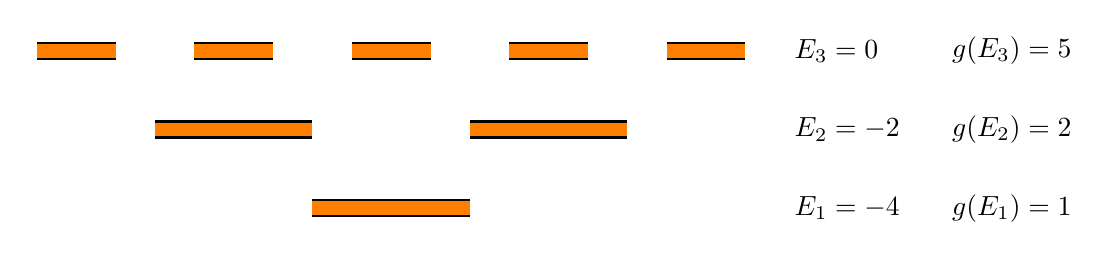
\begin{tikzpicture}
    \tikzset{level/.style   = {thick,
        double          = orange,
        double distance = 5pt}}
    
    \def\Espace{9};
    \def\Gspace{11};
    
    % Draw the energy levels.
    \draw[level] (3,0)  -- (5,0) node[right]{};
    \draw[] (\Espace,0) node[right] {$E_1=-4$};
    \draw[] (\Gspace,0) node[right] {$g(E_1)=1$};
    
    \draw[level] (1,1) -- (3,1) node[right] {};
    \draw[level] (5,1) -- (7,1) node[right] {};
    \draw[] (\Espace,1) node[right] {$E_2=-2$};
    \draw[] (\Gspace,1) node[right] {$g(E_2)=2$};
    
    \def\v{.5}; 
    \draw[level] (-1+\v,2) -- (0+\v,2) node[right] {};
    \draw[level] (1+\v,2) -- (2+\v,2) node[right] {};
    \draw[level] (3+\v,2) -- (4+\v,2) node[right] {};
    \draw[level] (5+\v,2) -- (6+\v,2) node[right] {};
    \draw[level] (7+\v,2) -- (8+\v,2) node[right] {};
    \draw[] (\Espace,2) node[right] {$E_3=0$};
    \draw[] (\Gspace,2) node[right] {$g(E_3)=5$};
  \end{tikzpicture}
}

\newcommand{\TIKZenergylevelSHORT}{

  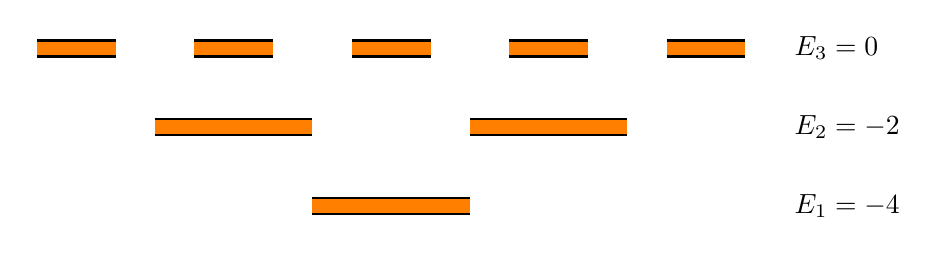
\begin{tikzpicture}
    \tikzset{level/.style   = {thick,
        double          = orange,
        double distance = 5pt,
        scale = 1.
        }}
    
    \def\Espace{9};
    \def\Gspace{11};
    
    % Draw the energy levels.
    \draw[level] (3,0)  -- (5,0) node[right]{};
    \draw[] (\Espace,0) node[right] {$E_1=-4$};
   
    \draw[level] (1,1) -- (3,1) node[right] {};
    \draw[level] (5,1) -- (7,1) node[right] {};
    \draw[] (\Espace,1) node[right] {$E_2=-2$};
    
    \def\v{.5}; 
    \draw[level] (-1+\v,2) -- (0+\v,2) node[right] {};
    \draw[level] (1+\v,2) -- (2+\v,2) node[right] {};
    \draw[level] (3+\v,2) -- (4+\v,2) node[right] {};
    \draw[level] (5+\v,2) -- (6+\v,2) node[right] {};
    \draw[level] (7+\v,2) -- (8+\v,2) node[right] {};
    \draw[] (\Espace,2) node[right] {$E_3=0$};
  \end{tikzpicture}
}


\newcommand{\TIKZgraphABC}{
  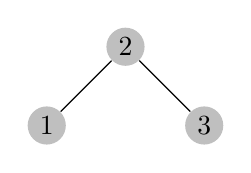
\begin{tikzpicture}[shorten >=1pt,->]
    \tikzstyle{vertex}=[circle,fill=black!25,minimum size=12pt,inner sep=2pt]
    \node[vertex] (G_1) at (-1,-1) {1};
    \node[vertex] (G_2) at (0,0)   {2};
    \node[vertex] (G_3) at (1,-1)  {3};
    \draw (G_1) -- (G_2) -- (G_3) -- cycle;
  \end{tikzpicture}
}

\newcommand{\TIKZgraphAB}{
  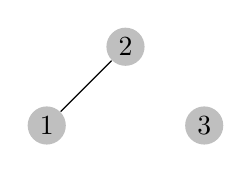
\begin{tikzpicture}[shorten >=1pt,->]
    \tikzstyle{vertex}=[circle,fill=black!25,minimum size=12pt,inner sep=2pt]
    \node[vertex] (G_1) at (-1,-1) {1};
    \node[vertex] (G_2) at (0,0)   {2};
    \node[vertex] (G_3) at (1,-1)  {3};
    \draw (G_1) -- (G_2) -- cycle;
  \end{tikzpicture}
}

\newcommand{\TIKZgraphBC}{
  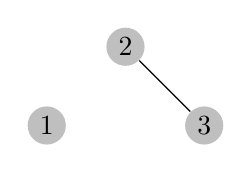
\begin{tikzpicture}[shorten >=1pt,->]
    \tikzstyle{vertex}=[circle,fill=black!25,minimum size=12pt,inner sep=2pt]
    \node[vertex] (G_1) at (-1,-1) {1};
    \node[vertex] (G_2) at (0,0)   {2};
    \node[vertex] (G_3) at (1,-1)  {3};
    \draw (G_2) -- (G_3) -- cycle;
  \end{tikzpicture}
}

\newcommand{\TIKZgraphC}{
  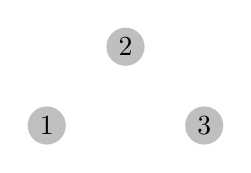
\begin{tikzpicture}[shorten >=1pt,->]
    \tikzstyle{vertex}=[circle,fill=black!25,minimum size=12pt,inner sep=2pt]
    \node[vertex] (G_1) at (-1,-1) {1};
    \node[vertex] (G_2) at (0,0)   {2};
    \node[vertex] (G_3) at (1,-1)  {3};
  \end{tikzpicture}
}


\newcommand{\TIKZgraphoneline}{
  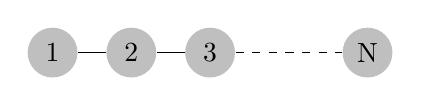
\begin{tikzpicture}[shorten >=1pt,->]
    \tikzstyle{vertex}=[circle,fill=black!25,minimum size=18pt,inner sep=2pt]
    \node[vertex] (G1) at (0,0)   {1};
    \node[vertex] (G2) at (1,0)   {2};
    \node[vertex] (G3) at (2,0)   {3};
    \node[vertex] (GN) at (4,0)   {N};
    \draw (G1) -- (G2) -- (G3) -- cycle;
    \draw[dashed] (G3) -- (GN) -- cycle;
  \end{tikzpicture}
}


\newcommand{\TIKZgraphtwoline}{
  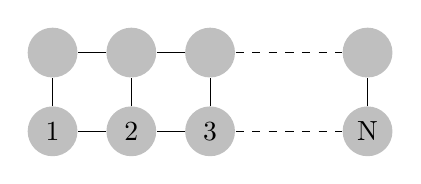
\begin{tikzpicture}[shorten >=1pt,->]
    \tikzstyle{vertex}=[circle,fill=black!25,minimum size=18pt,inner sep=2pt]
    \node[vertex] (G1) at (0,0)   {1};
    \node[vertex] (G2) at (1,0)   {2};
    \node[vertex] (G3) at (2,0)   {3};
    \node[vertex] (GN) at (4,0)   {N};
    \draw (G1) -- (G2) -- (G3) -- cycle;
    \draw[dashed] (G3) -- (GN) -- cycle;

    \node[vertex] (GN1) at (0,1)   {};
    \node[vertex] (GN2) at (1,1)   {};
    \node[vertex] (GN3) at (2,1)   {};
    \node[vertex] (G2N) at (4,1)   {};
    
    \draw (GN1) -- (GN2) -- (GN3) -- cycle;
    \draw (GN) -- (G2N) -- cycle;
    \draw (G1) -- (GN1) -- cycle;
    \draw (G2) -- (GN2) -- cycle;
    \draw (G3) -- (GN3) -- cycle;
    \draw (GN) -- (G2N) -- cycle;

    \draw[dashed] (GN3) -- (G2N) -- cycle;


  \end{tikzpicture}
}



\newcommand{\TIKZtwoladdera}{
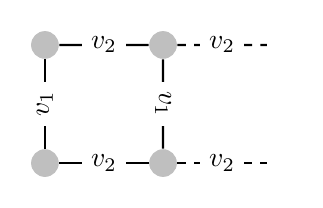
\begin{tikzpicture}[scale=\tikzpicscale]
    \node[vertex] (G1) at (0,0)   {};
    \node[vertex] (G2) at (1,0)   {};
    \node[vertex] (GA) at (0,1)   {};
    \node[vertex] (GB) at (1,1)   {};
	 \Edge[label=$v_2$](G1)(G2)
	 \Edge[label=$v_2$](GA)(GB)
	 \Edge[label=$v_1$](G1)(GA)
	 \Edge[label=$v_1$](G2)(GB)
    \node[Nvertex] (G3) at (2,0)   {};
    \node[Nvertex] (GC) at (2,1)   {};
	 \tikzstyle{EdgeStyle}=[dashed]
	 \Edge[label=$v_2$](G2)(G3)
	 \Edge[label=$v_2$](GB)(GC)
\end{tikzpicture}
}

\newcommand{\TIKZtwoladderb}{
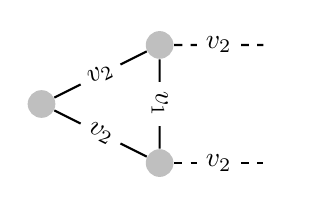
\begin{tikzpicture}[scale=\tikzpicscale]
    \node[vertex] (G2) at (1,0)   {};
    \node[vertex] (GB) at (1,1)   {};
    \node[vertex] (G1A) at (0,.5)   {};
	 \Edge[label=$v_2$](G1A)(G2)
	 \Edge[label=$v_2$](G1A)(GB)
	 \Edge[label=$v_1$](G2)(GB)
    \node[Nvertex] (G3) at (2,0)   {};
    \node[Nvertex] (GC) at (2,1)   {};
	 \tikzstyle{EdgeStyle}=[dashed]
	 \Edge[label=$v_2$](G2)(G3)
	 \Edge[label=$v_2$](GB)(GC)
\end{tikzpicture}
}

\newcommand{\TIKZtwoladderc}{
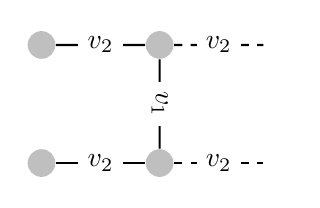
\begin{tikzpicture}[scale=\tikzpicscale]
    \node[vertex] (G1) at (0,0)   {};
    \node[vertex] (G2) at (1,0)   {};
    \node[vertex] (GA) at (0,1)   {};
    \node[vertex] (GB) at (1,1)   {};
	 \Edge[label=$v_2$](G1)(G2)
	 \Edge[label=$v_2$](GA)(GB)
	 %\Edge[label=$v_1$](G1)(GA)
	 \Edge[label=$v_1$](G2)(GB)
    \node[Nvertex] (G3) at (2,0)   {};
    \node[Nvertex] (GC) at (2,1)   {};
	 \tikzstyle{EdgeStyle}=[dashed]
	 \Edge[label=$v_2$](G2)(G3)
	 \Edge[label=$v_2$](GB)(GC)
\end{tikzpicture}
}

\newcommand{\TIKZtwoladderd}{
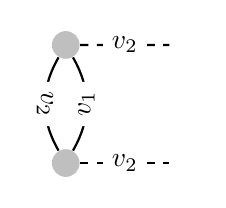
\begin{tikzpicture}[scale=\tikzpicscale]
    \node[vertex] (G2) at (1,0)   {};
    \node[vertex] (GB) at (1,1)   {};
	 %\Edge[label=$v_1$](G1)(GA)
	\tikzstyle{EdgeStyle}=[bend left]
	\Edge[label=$v_2$](G2)(GB)
  	\tikzstyle{EdgeStyle}=[bend right]
	\Edge[label=$v_1$](G2)(GB)
    \node[Nvertex] (G3) at (2,0)   {};
    \node[Nvertex] (GC) at (2,1)   {};
	 \tikzstyle{EdgeStyle}=[dashed]
	 \Edge[label=$v_2$](G2)(G3)
	 \Edge[label=$v_2$](GB)(GC)
\end{tikzpicture}
}

\newcommand{\TIKZtwoladdere}{
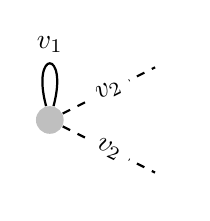
\begin{tikzpicture}[scale=\tikzpicscale]
    \node[vertex] (G2B) at (1,.5)   {};
	 %\Edge[label=$v_1$](G1)(GA)
	\tikzstyle{EdgeStyle}=[loop above]
	\Edge[label=$v_1$](G2B)(G2B)
   \node[Nvertex] (G3) at (2,0)   {};
   \node[Nvertex] (GC) at (2,1)   {};
	\tikzstyle{EdgeStyle}=[dashed]
	\Edge[label=$v_2$](G2B)(G3)
	\Edge[label=$v_2$](G2B)(GC)
\end{tikzpicture}
}

\newcommand{\TIKZtwoladderf}{
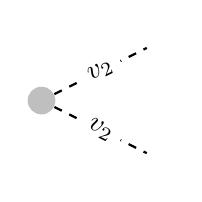
\begin{tikzpicture}[scale=\tikzpicscale]
    \node[vertex] (G2B) at (1,.5)   {};
   \node[Nvertex] (G3) at (2,0)   {};
   \node[Nvertex] (GC) at (2,1)   {};
	\tikzstyle{EdgeStyle}=[dashed]
	\Edge[label=$v_2$](G2B)(G3)
	\Edge[label=$v_2$](G2B)(GC)
\end{tikzpicture}
}

\newcommand{\TIKZthreeladderA}{
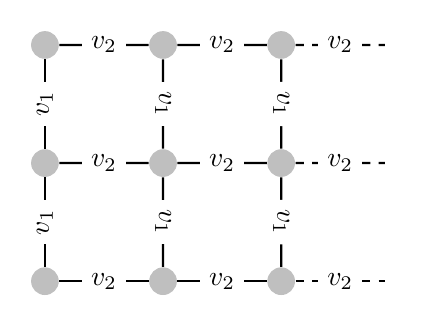
\begin{tikzpicture}[scale=\tikzpicscale]
    \node[vertex] (00) at (0,0)   {};
    \node[vertex] (10) at (1,0)   {};
	 \node[vertex] (20) at (2,0)   {};
    \node[vertex] (01) at (0,1)   {};
    \node[vertex] (11) at (1,1)   {};
    \node[vertex] (21) at (2,1)   {};
    \node[vertex] (02) at (0,2)   {};
    \node[vertex] (12) at (1,2)   {};
    \node[vertex] (22) at (2,2)   {};
	 \Edge[label=$v_2$](00)(10)
	 \Edge[label=$v_2$](10)(20)
	 \Edge[label=$v_2$](01)(11)
	 \Edge[label=$v_2$](11)(21)
	 \Edge[label=$v_2$](02)(12)
	 \Edge[label=$v_2$](12)(22)	
	 \Edge[label=$v_1$](00)(01)
	 \Edge[label=$v_1$](10)(11)
	 \Edge[label=$v_1$](20)(21)
 	 \Edge[label=$v_1$](21)(22)
 	 \Edge[label=$v_1$](11)(12)
 	 \Edge[label=$v_1$](01)(02)
    \node[Nvertex] (n30) at (3,0)   {};
    \node[Nvertex] (n31) at (3,1)   {};
    \node[Nvertex] (n32) at (3,2)   {};
	 \tikzstyle{EdgeStyle}=[dashed]
	 \Edge[label=$v_2$](20)(n30)
	 \Edge[label=$v_2$](21)(n31)
 	 \Edge[label=$v_2$](22)(n32)
\end{tikzpicture}
}

\newcommand{\TIKZthreeladderB}{
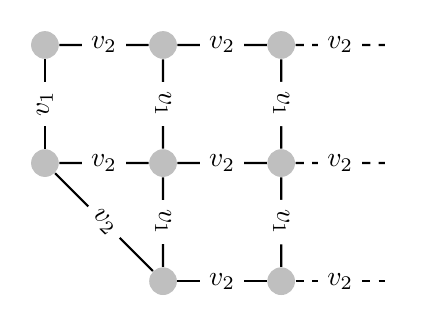
\begin{tikzpicture}[scale=\tikzpicscale]
%    \node[vertex] (00) at (0,0)   {};
    \node[vertex] (10) at (1,0)   {};
	 \node[vertex] (20) at (2,0)   {};
    \node[vertex] (01) at (0,1)   {};
    \node[vertex] (11) at (1,1)   {};
    \node[vertex] (21) at (2,1)   {};
    \node[vertex] (02) at (0,2)   {};
    \node[vertex] (12) at (1,2)   {};
    \node[vertex] (22) at (2,2)   {};
	 \Edge[label=$v_2$](01)(10)
	 \Edge[label=$v_2$](10)(20)
	 \Edge[label=$v_2$](01)(11)
	 \Edge[label=$v_2$](11)(21)
	 \Edge[label=$v_2$](02)(12)
	 \Edge[label=$v_2$](12)(22)	
%)	 \Edge[label=$v_1$](00)(01)
	 \Edge[label=$v_1$](10)(11)
	 \Edge[label=$v_1$](20)(21)
 	 \Edge[label=$v_1$](21)(22)
 	 \Edge[label=$v_1$](11)(12)
 	 \Edge[label=$v_1$](01)(02)
    \node[Nvertex] (n30) at (3,0)   {};
    \node[Nvertex] (n31) at (3,1)   {};
    \node[Nvertex] (n32) at (3,2)   {};
	 \tikzstyle{EdgeStyle}=[dashed]
	 \Edge[label=$v_2$](20)(n30)
	 \Edge[label=$v_2$](21)(n31)
 	 \Edge[label=$v_2$](22)(n32)
\end{tikzpicture}
}

\newcommand{\TIKZthreeladderC}{
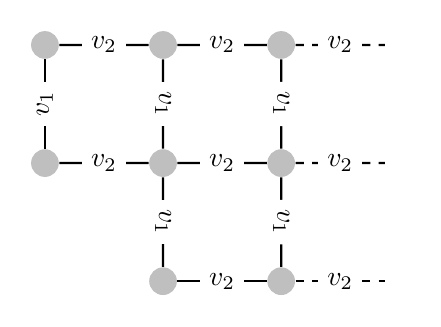
\begin{tikzpicture}[scale=\tikzpicscale]
%    \node[vertex] (00) at (0,0)   {};
    \node[vertex] (10) at (1,0)   {};
	 \node[vertex] (20) at (2,0)   {};
    \node[vertex] (01) at (0,1)   {};
    \node[vertex] (11) at (1,1)   {};
    \node[vertex] (21) at (2,1)   {};
    \node[vertex] (02) at (0,2)   {};
    \node[vertex] (12) at (1,2)   {};
    \node[vertex] (22) at (2,2)   {};
%	 \Edge[label=$v_2$](01)(10)
	 \Edge[label=$v_2$](10)(20)
	 \Edge[label=$v_2$](01)(11)
	 \Edge[label=$v_2$](11)(21)
	 \Edge[label=$v_2$](02)(12)
	 \Edge[label=$v_2$](12)(22)	
%)	 \Edge[label=$v_1$](00)(01)
	 \Edge[label=$v_1$](10)(11)
	 \Edge[label=$v_1$](20)(21)
 	 \Edge[label=$v_1$](21)(22)
 	 \Edge[label=$v_1$](11)(12)
 	 \Edge[label=$v_1$](01)(02)
    \node[Nvertex] (n30) at (3,0)   {};
    \node[Nvertex] (n31) at (3,1)   {};
    \node[Nvertex] (n32) at (3,2)   {};
	 \tikzstyle{EdgeStyle}=[dashed]
	 \Edge[label=$v_2$](20)(n30)
	 \Edge[label=$v_2$](21)(n31)
 	 \Edge[label=$v_2$](22)(n32)
\end{tikzpicture}
}

\newcommand{\TIKZthreeladderD}{
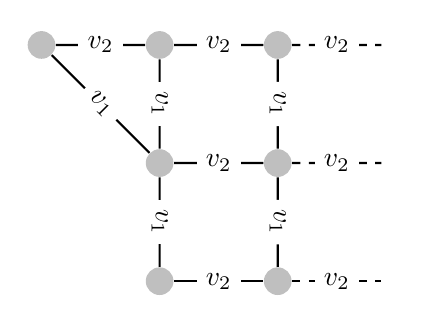
\begin{tikzpicture}[scale=\tikzpicscale]
%    \node[vertex] (00) at (0,0)   {};
    \node[vertex] (10) at (1,0)   {};
	 \node[vertex] (20) at (2,0)   {};
%    \node[vertex] (01) at (0,1)   {};
    \node[vertex] (11) at (1,1)   {};
    \node[vertex] (21) at (2,1)   {};
    \node[vertex] (02) at (0,2)   {};
    \node[vertex] (12) at (1,2)   {};
    \node[vertex] (22) at (2,2)   {};
%	 \Edge[label=$v_2$](01)(10)
	 \Edge[label=$v_2$](10)(20)
%	 \Edge[label=$v_2$](01)(11)
	 \Edge[label=$v_2$](11)(21)
	 \Edge[label=$v_2$](02)(12)
	 \Edge[label=$v_2$](12)(22)	
%)	 \Edge[label=$v_1$](00)(01)
	 \Edge[label=$v_1$](10)(11)
	 \Edge[label=$v_1$](20)(21)
 	 \Edge[label=$v_1$](21)(22)
 	 \Edge[label=$v_1$](11)(12)
 	 \Edge[label=$v_1$](11)(02)
    \node[Nvertex] (n30) at (3,0)   {};
    \node[Nvertex] (n31) at (3,1)   {};
    \node[Nvertex] (n32) at (3,2)   {};
	 \tikzstyle{EdgeStyle}=[dashed]
	 \Edge[label=$v_2$](20)(n30)
	 \Edge[label=$v_2$](21)(n31)
 	 \Edge[label=$v_2$](22)(n32)
\end{tikzpicture}
}

\newcommand{\TIKZthreeladderE}{
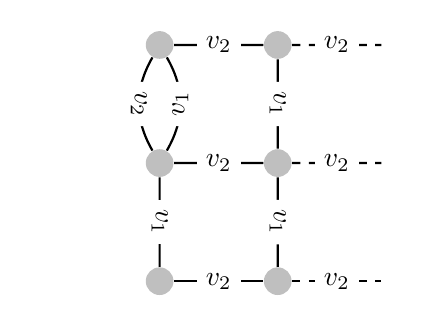
\begin{tikzpicture}[scale=\tikzpicscale]
    \node[Nvertex] (00) at (0,0)   {};
    \node[vertex] (10) at (1,0)   {};
	 \node[vertex] (20) at (2,0)   {};
%    \node[vertex] (01) at (0,1)   {};
    \node[vertex] (11) at (1,1)   {};
    \node[vertex] (21) at (2,1)   {};
%    \node[vertex] (02) at (0,2)   {};
    \node[vertex] (12) at (1,2)   {};
    \node[vertex] (22) at (2,2)   {};
%	 \Edge[label=$v_2$](01)(10)
	 \Edge[label=$v_2$](10)(20)
%	 \Edge[label=$v_2$](01)(11)
	 \Edge[label=$v_2$](11)(21)
%	 \Edge[label=$v_2$](02)(12)
	 \Edge[label=$v_2$](12)(22)	
%)	 \Edge[label=$v_1$](00)(01)
	 \Edge[label=$v_1$](10)(11)
	 \Edge[label=$v_1$](20)(21)
 	 \Edge[label=$v_1$](21)(22)
% 	 \Edge[label=$v_1$](11)(02)
    \node[Nvertex] (n30) at (3,0)   {};
    \node[Nvertex] (n31) at (3,1)   {};
    \node[Nvertex] (n32) at (3,2)   {};
	 \tikzstyle{EdgeStyle}=[dashed]
	 \Edge[label=$v_2$](20)(n30)
	 \Edge[label=$v_2$](21)(n31)
 	 \Edge[label=$v_2$](22)(n32)
 	 \tikzstyle{EdgeStyle}=[bend left]
  	 \Edge[label=$v_2$](11)(12)
  	 \tikzstyle{EdgeStyle}=[bend right]
  	 \Edge[label=$v_1$](11)(12)
\end{tikzpicture}
}

\newcommand{\TIKZthreeladderF}{
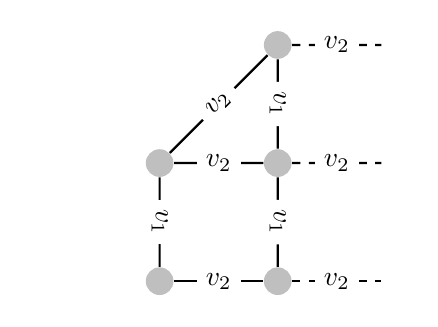
\begin{tikzpicture}[scale=\tikzpicscale]
    \node[Nvertex] (00) at (0,0)   {};
    \node[vertex] (10) at (1,0)   {};
	 \node[vertex] (20) at (2,0)   {};
%    \node[vertex] (01) at (0,1)   {};
    \node[vertex] (11) at (1,1)   {};
    \node[vertex] (21) at (2,1)   {};
%    \node[vertex] (02) at (0,2)   {};
%    \node[vertex] (12) at (1,2)   {};
    \node[vertex] (22) at (2,2)   {};
%	 \Edge[label=$v_2$](01)(10)
	 \Edge[label=$v_2$](10)(20)
%	 \Edge[label=$v_2$](01)(11)
	 \Edge[label=$v_2$](11)(21)
%	 \Edge[label=$v_2$](02)(12)
	 \Edge[label=$v_2$](11)(22)	
%)	 \Edge[label=$v_1$](00)(01)
	 \Edge[label=$v_1$](10)(11)
	 \Edge[label=$v_1$](20)(21)
 	 \Edge[label=$v_1$](21)(22)
% 	 \Edge[label=$v_1$](11)(02)
    \node[Nvertex] (n30) at (3,0)   {};
    \node[Nvertex] (n31) at (3,1)   {};
    \node[Nvertex] (n32) at (3,2)   {};
	 \tikzstyle{EdgeStyle}=[dashed]
	 \Edge[label=$v_2$](20)(n30)
	 \Edge[label=$v_2$](21)(n31)
 	 \Edge[label=$v_2$](22)(n32)
  	 %\tikzstyle{EdgeStyle}=[loop above]
  	 %\Edge[label=$v_1$](11)(11)
\end{tikzpicture}
}

\newcommand{\TIKZthreeladderG}{
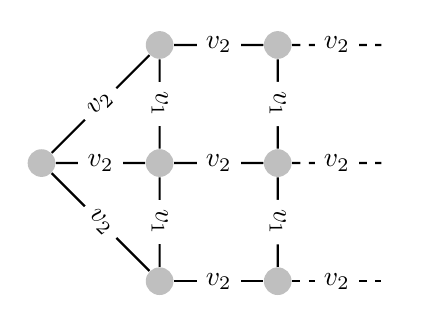
\begin{tikzpicture}[scale=\tikzpicscale]
%    \node[vertex] (00) at (0,0)   {};
    \node[vertex] (10) at (1,0)   {};
	 \node[vertex] (20) at (2,0)   {};
    \node[vertex] (01) at (0,1)   {};
    \node[vertex] (11) at (1,1)   {};
    \node[vertex] (21) at (2,1)   {};
%    \node[vertex] (02) at (0,2)   {};
    \node[vertex] (12) at (1,2)   {};
    \node[vertex] (22) at (2,2)   {};
	 \Edge[label=$v_2$](01)(10)
	 \Edge[label=$v_2$](10)(20)
	 \Edge[label=$v_2$](01)(11)
	 \Edge[label=$v_2$](11)(21)
	 \Edge[label=$v_2$](01)(12)
	 \Edge[label=$v_2$](12)(22)	
%)	 \Edge[label=$v_1$](00)(01)
	 \Edge[label=$v_1$](10)(11)
	 \Edge[label=$v_1$](20)(21)
 	 \Edge[label=$v_1$](21)(22)
 	 \Edge[label=$v_1$](11)(12)
% 	 \Edge[label=$v_1$](01)(02)
    \node[Nvertex] (n30) at (3,0)   {};
    \node[Nvertex] (n31) at (3,1)   {};
    \node[Nvertex] (n32) at (3,2)   {};
	 \tikzstyle{EdgeStyle}=[dashed]
	 \Edge[label=$v_2$](20)(n30)
	 \Edge[label=$v_2$](21)(n31)
 	 \Edge[label=$v_2$](22)(n32)
\end{tikzpicture}
}

\newcommand{\TIKZthreeladderH}{
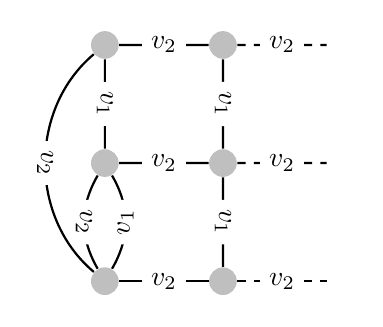
\begin{tikzpicture}[scale=\tikzpicscale]
%    \node[vertex] (00) at (0,0)   {};
    \node[vertex] (10) at (1,0)   {};
	 \node[vertex] (20) at (2,0)   {};
%    \node[vertex] (01) at (0,1)   {};
    \node[vertex] (11) at (1,1)   {};
    \node[vertex] (21) at (2,1)   {};
%    \node[vertex] (02) at (0,2)   {};
    \node[vertex] (12) at (1,2)   {};
    \node[vertex] (22) at (2,2)   {};
	 \Edge[label=$v_2$](10)(20)
%	 \Edge[label=$v_2$](01)(11)
	 \Edge[label=$v_2$](11)(21)
%	 \Edge[label=$v_2$](01)(12)
	 \Edge[label=$v_2$](12)(22)	
%)	 \Edge[label=$v_1$](00)(01)
	 \Edge[label=$v_1$](20)(21)
 	 \Edge[label=$v_1$](21)(22)
 	 \Edge[label=$v_1$](11)(12)
% 	 \Edge[label=$v_1$](01)(02)
    \node[Nvertex] (n30) at (3,0)   {};
    \node[Nvertex] (n31) at (3,1)   {};
    \node[Nvertex] (n32) at (3,2)   {};
	 \tikzstyle{EdgeStyle}=[dashed]
	 \Edge[label=$v_2$](20)(n30)
	 \Edge[label=$v_2$](21)(n31)
 	 \Edge[label=$v_2$](22)(n32)
 	 
 	 \tikzstyle{EdgeStyle}=[bend left]
 	 \Edge[label=$v_2$](10)(11)
  	 \tikzstyle{EdgeStyle}=[bend left=50]
 	 \Edge[label=$v_2$](10)(12)
  	 %\Edge[label=$v_2$](11)(12)
 	 \tikzstyle{EdgeStyle}=[bend right]
	 \Edge[label=$v_1$](10)(11)
\end{tikzpicture}
}

\newcommand{\TIKZthreeladderI}{
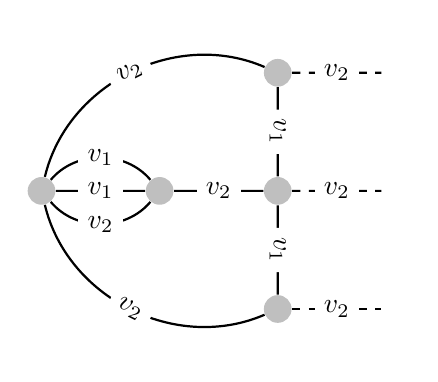
\begin{tikzpicture}[scale=\tikzpicscale]
%    \node[vertex] (00) at (0,0)   {};
%    \node[vertex] (10) at (1,0)   {};
	 \node[vertex] (20) at (2,0)   {};
    \node[vertex] (01) at (0,1)   {};
    \node[vertex] (11) at (1,1)   {};
    \node[vertex] (21) at (2,1)   {};
%    \node[vertex] (02) at (0,2)   {};
%    \node[vertex] (12) at (1,2)   {};
    \node[vertex] (22) at (2,2)   {};
%	 \Edge[label=$v_2$](01)(10)
%	 \Edge[label=$v_2$](10)(20)
%	 \Edge[label=$v_2$](01)(21)
	 \Edge[label=$v_2$](11)(21)
%	 \Edge[label=$v_2$](12)(22)	
%)	 \Edge[label=$v_1$](00)(01)
%	 \Edge[label=$v_1$](10)(11)
	 \Edge[label=$v_1$](20)(21)
 	 \Edge[label=$v_1$](21)(22)
% 	 \Edge[label=$v_1$](11)(12)
% 	 \Edge[label=$v_1$](01)(02)
    \node[Nvertex] (n30) at (3,0)   {};
    \node[Nvertex] (n31) at (3,1)   {};
    \node[Nvertex] (n32) at (3,2)   {};
	 \tikzstyle{EdgeStyle}=[dashed]
	 \Edge[label=$v_2$](20)(n30)
	 \Edge[label=$v_2$](21)(n31)
 	 \Edge[label=$v_2$](22)(n32)

	 \tikzstyle{EdgeStyle}=[]
	 \Edge[label=$v_1$](01)(11)
  	 \tikzstyle{EdgeStyle}=[bend left=50]
	 \Edge[label=$v_2$](01)(22)
 	 \Edge[label=$v_1$](01)(11)
  	 \tikzstyle{EdgeStyle}=[bend right=50]
 	 \Edge[label=$v_2$](01)(20)
 	 \Edge[label=$v_2$](01)(11)
\end{tikzpicture}
}


\newcommand{\TIKZthreeladderJ}{
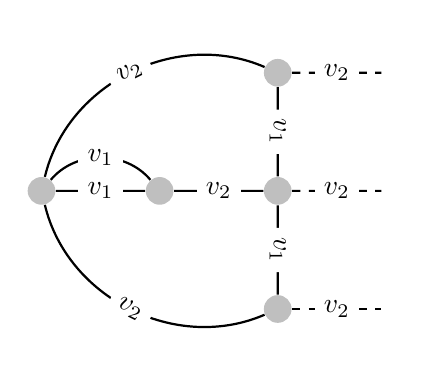
\begin{tikzpicture}[scale=\tikzpicscale]
%    \node[vertex] (00) at (0,0)   {};
%    \node[vertex] (10) at (1,0)   {};
	 \node[vertex] (20) at (2,0)   {};
    \node[vertex] (01) at (0,1)   {};
    \node[vertex] (11) at (1,1)   {};
    \node[vertex] (21) at (2,1)   {};
%    \node[vertex] (02) at (0,2)   {};
%    \node[vertex] (12) at (1,2)   {};
    \node[vertex] (22) at (2,2)   {};
%	 \Edge[label=$v_2$](01)(10)
%	 \Edge[label=$v_2$](10)(20)
%	 \Edge[label=$v_2$](01)(21)
	 \Edge[label=$v_2$](11)(21)
%	 \Edge[label=$v_2$](12)(22)	
%)	 \Edge[label=$v_1$](00)(01)
%	 \Edge[label=$v_1$](10)(11)
	 \Edge[label=$v_1$](20)(21)
 	 \Edge[label=$v_1$](21)(22)
% 	 \Edge[label=$v_1$](11)(12)
% 	 \Edge[label=$v_1$](01)(02)
    \node[Nvertex] (n30) at (3,0)   {};
    \node[Nvertex] (n31) at (3,1)   {};
    \node[Nvertex] (n32) at (3,2)   {};
	 \tikzstyle{EdgeStyle}=[dashed]
	 \Edge[label=$v_2$](20)(n30)
	 \Edge[label=$v_2$](21)(n31)
 	 \Edge[label=$v_2$](22)(n32)

	 \tikzstyle{EdgeStyle}=[]
	 \Edge[label=$v_1$](01)(11)
  	 \tikzstyle{EdgeStyle}=[bend left=50]
	 \Edge[label=$v_2$](01)(22)
 	 \Edge[label=$v_1$](01)(11)
  	 \tikzstyle{EdgeStyle}=[bend right=50]
 	 \Edge[label=$v_2$](01)(20)
% 	 \Edge[label=$v_2$](01)(11)
\end{tikzpicture}
}

\newcommand{\TIKZoneladderA}{
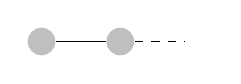
\begin{tikzpicture}[shorten >=1pt,->]
    \tikzstyle{vertex}=[circle,fill=black!25,minimum size=10pt,inner sep=2pt]
    \tikzstyle{nullvertex}=[circle,fill=white!25,minimum size=10pt,inner sep=2pt]
    \node[vertex] (G1) at (0,0)   {};
    \node[vertex] (G2) at (1,0)   {};
    \node[nullvertex] (GX) at (2,0)   {};
    \draw (G1) -- (G2) -- cycle;
    \draw[dashed] (G2) -- (GX) -- cycle;
\end{tikzpicture}
}

\newcommand{\TIKZoneladderB}{
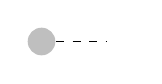
\begin{tikzpicture}[shorten >=1pt,->]
    \tikzstyle{vertex}=[circle,fill=black!25,minimum size=10pt,inner sep=2pt]
    \tikzstyle{nullvertex}=[circle,fill=white!25,minimum size=10pt,inner sep=2pt]
    \node[vertex] (G2) at (1,0)   {};
    \node[nullvertex] (GX) at (2,0)   {};
    \draw[dashed] (G2) -- (GX) -- cycle;
\end{tikzpicture}
}

\newcommand{\TIKZoneladderC}{

\begin{tikzpicture}[shorten >=1pt,->]
    \tikzstyle{vertex}=[circle,fill=black!25,minimum size=10pt,inner sep=2pt]
    \tikzstyle{nullvertex}=[circle,fill=white!25,minimum size=10pt,inner sep=2pt]
    \node[vertex] (G1) at (0,0)   {};
    \node[vertex] (G2) at (1,0)   {};
    \node[nullvertex] (GX) at (2,0)   {};
    %\draw (G1) -- (G2) -- cycle;
    \draw[dashed] (G2) -- (GX) -- cycle;
\end{tikzpicture}
}

\newcommand{\TIKZpetersengraph} {
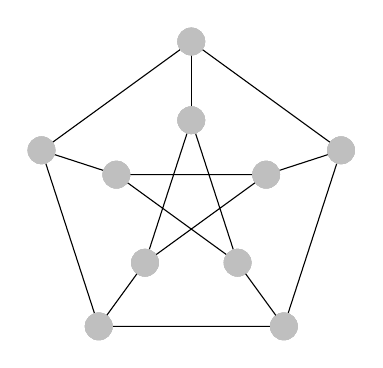
\begin{tikzpicture}[]
    \tikzstyle{vertex}=[circle,fill=black!25,minimum size=10pt,inner sep=2pt]
            
\draw (18:2cm) -- (90:2cm) -- (162:2cm) -- (234:2cm) -- (306:2cm) -- cycle;
\draw (18:1cm) -- (162:1cm) -- (306:1cm) -- (90:1cm) -- (234:1cm) -- cycle;
\foreach \x in {18,90,162,234,306}{
\draw (\x:1cm) -- (\x:2cm);

    \node[vertex] at (18:2cm) {};
    \node[vertex] at (90:2cm) {};
    \node[vertex] at (162:2cm) {};
    \node[vertex] at (234:2cm) {};
    \node[vertex] at (306:2cm) {};
    \node[vertex] at (18:1cm) {};
    \node[vertex] at (162:1cm) {};
    \node[vertex] at (306:1cm) {};
    \node[vertex] at (90:1cm) {};
    \node[vertex] at (234:1cm) {};

%\draw (\x:2cm) circle (2pt);
%\draw (\x:1cm) circle (2pt);
}
\end{tikzpicture}
}

\newcommand{\TIKZFLWmacrostates} {

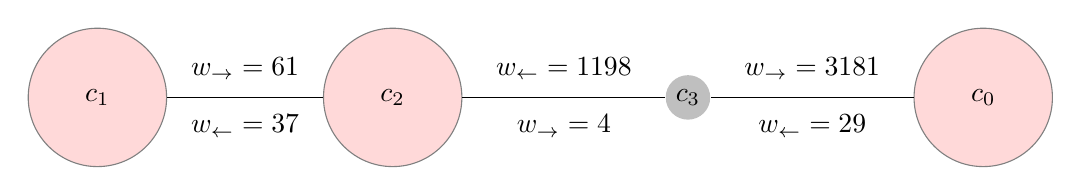
\begin{tikzpicture}[scale=\tikzpicscale]

  \node[big_vertex] (c1) at (0,0)   {$c_1$};
  \node[big_vertex] (c2) at (1*\vertexshiftamount,0)   {$c_2$};
  \node[vertex]    (c3) at (2*\vertexshiftamount,0)   {$c_3$};
  \node[big_vertex] (c0) at (3*\vertexshiftamount,0)   {$c_0$};
  
  \draw [] (c0) -> node[above=.1cm] {$w_{\rightarrow}=3181$} (c3);
  \draw [] (c0) -> node[below=.1cm] {$w_{\leftarrow}=29$} (c3);

  \draw [] (c2) -> node[above=.1cm] {$w_{\leftarrow}=1198$} (c3);  
  \draw [] (c2) -> node[below=.1cm] {$w_{\rightarrow}=4$} (c3);
  
  \draw [] (c2) -- node[below=.1cm] {$w_{\leftarrow}=37$} (c1);
  \draw [] (c2) -- node[above=.1cm] {$w_{\rightarrow}=61$} (c1);
\end{tikzpicture}
}

\newcommand{\TIKZbetahairpinNativestate} {
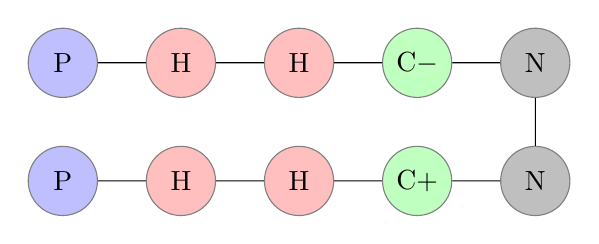
\begin{tikzpicture}[scale=\tikzpicscale]
    \tikzstyle{hvertex}=[circle,fill=red!25,minimum size=25pt,inner sep=2pt,draw=black!50]
    \tikzstyle{pvertex}=[circle,fill=blue!25,minimum size=25pt,inner sep=2pt,draw=black!50]
    \tikzstyle{cpvertex}=[circle,fill=green!25,minimum size=25pt,inner sep=2pt,draw=black!50]
    \tikzstyle{nvertex}=[circle,fill=black!25,minimum size=25pt,inner sep=2pt,draw=black!50]

    \node[pvertex] (r0) at (0,0)   {\chem{P}};
    \node[hvertex] (r1) at (1,0)   {\chem{H}};
    \node[hvertex] (r2) at (2,0)   {\chem{H}};
    \node[cpvertex] (r3) at (3,0)   {\chem{C+}};
    \node[nvertex] (r4) at (4,0)   {\chem{N}};
    \node[nvertex] (r5) at (4,1)   {\chem{N}};
    \node[cpvertex] (r6) at (3,1)   {\chem{C-}};
    \node[hvertex] (r7) at (2,1)   {\chem{H}};
    \node[hvertex] (r8) at (1,1)   {\chem{H}};
    \node[pvertex] (r9) at (0,1)   {\chem{P}};

    \draw [] (r0)--(r1)--(r2)--(r3)--(r4)--(r5)--(r6)--(r7)--(r8)--(r9)--cycle;
   
\end{tikzpicture}
}


\newcommand{\TIKZbetahairpinMacrostates} {
\begin{tikzpicture}[scale=\tikzpicscale]
    \node[macrostate_vertex] (R) at (0,0)   {
    \begin{minipage}{3.1cm}
    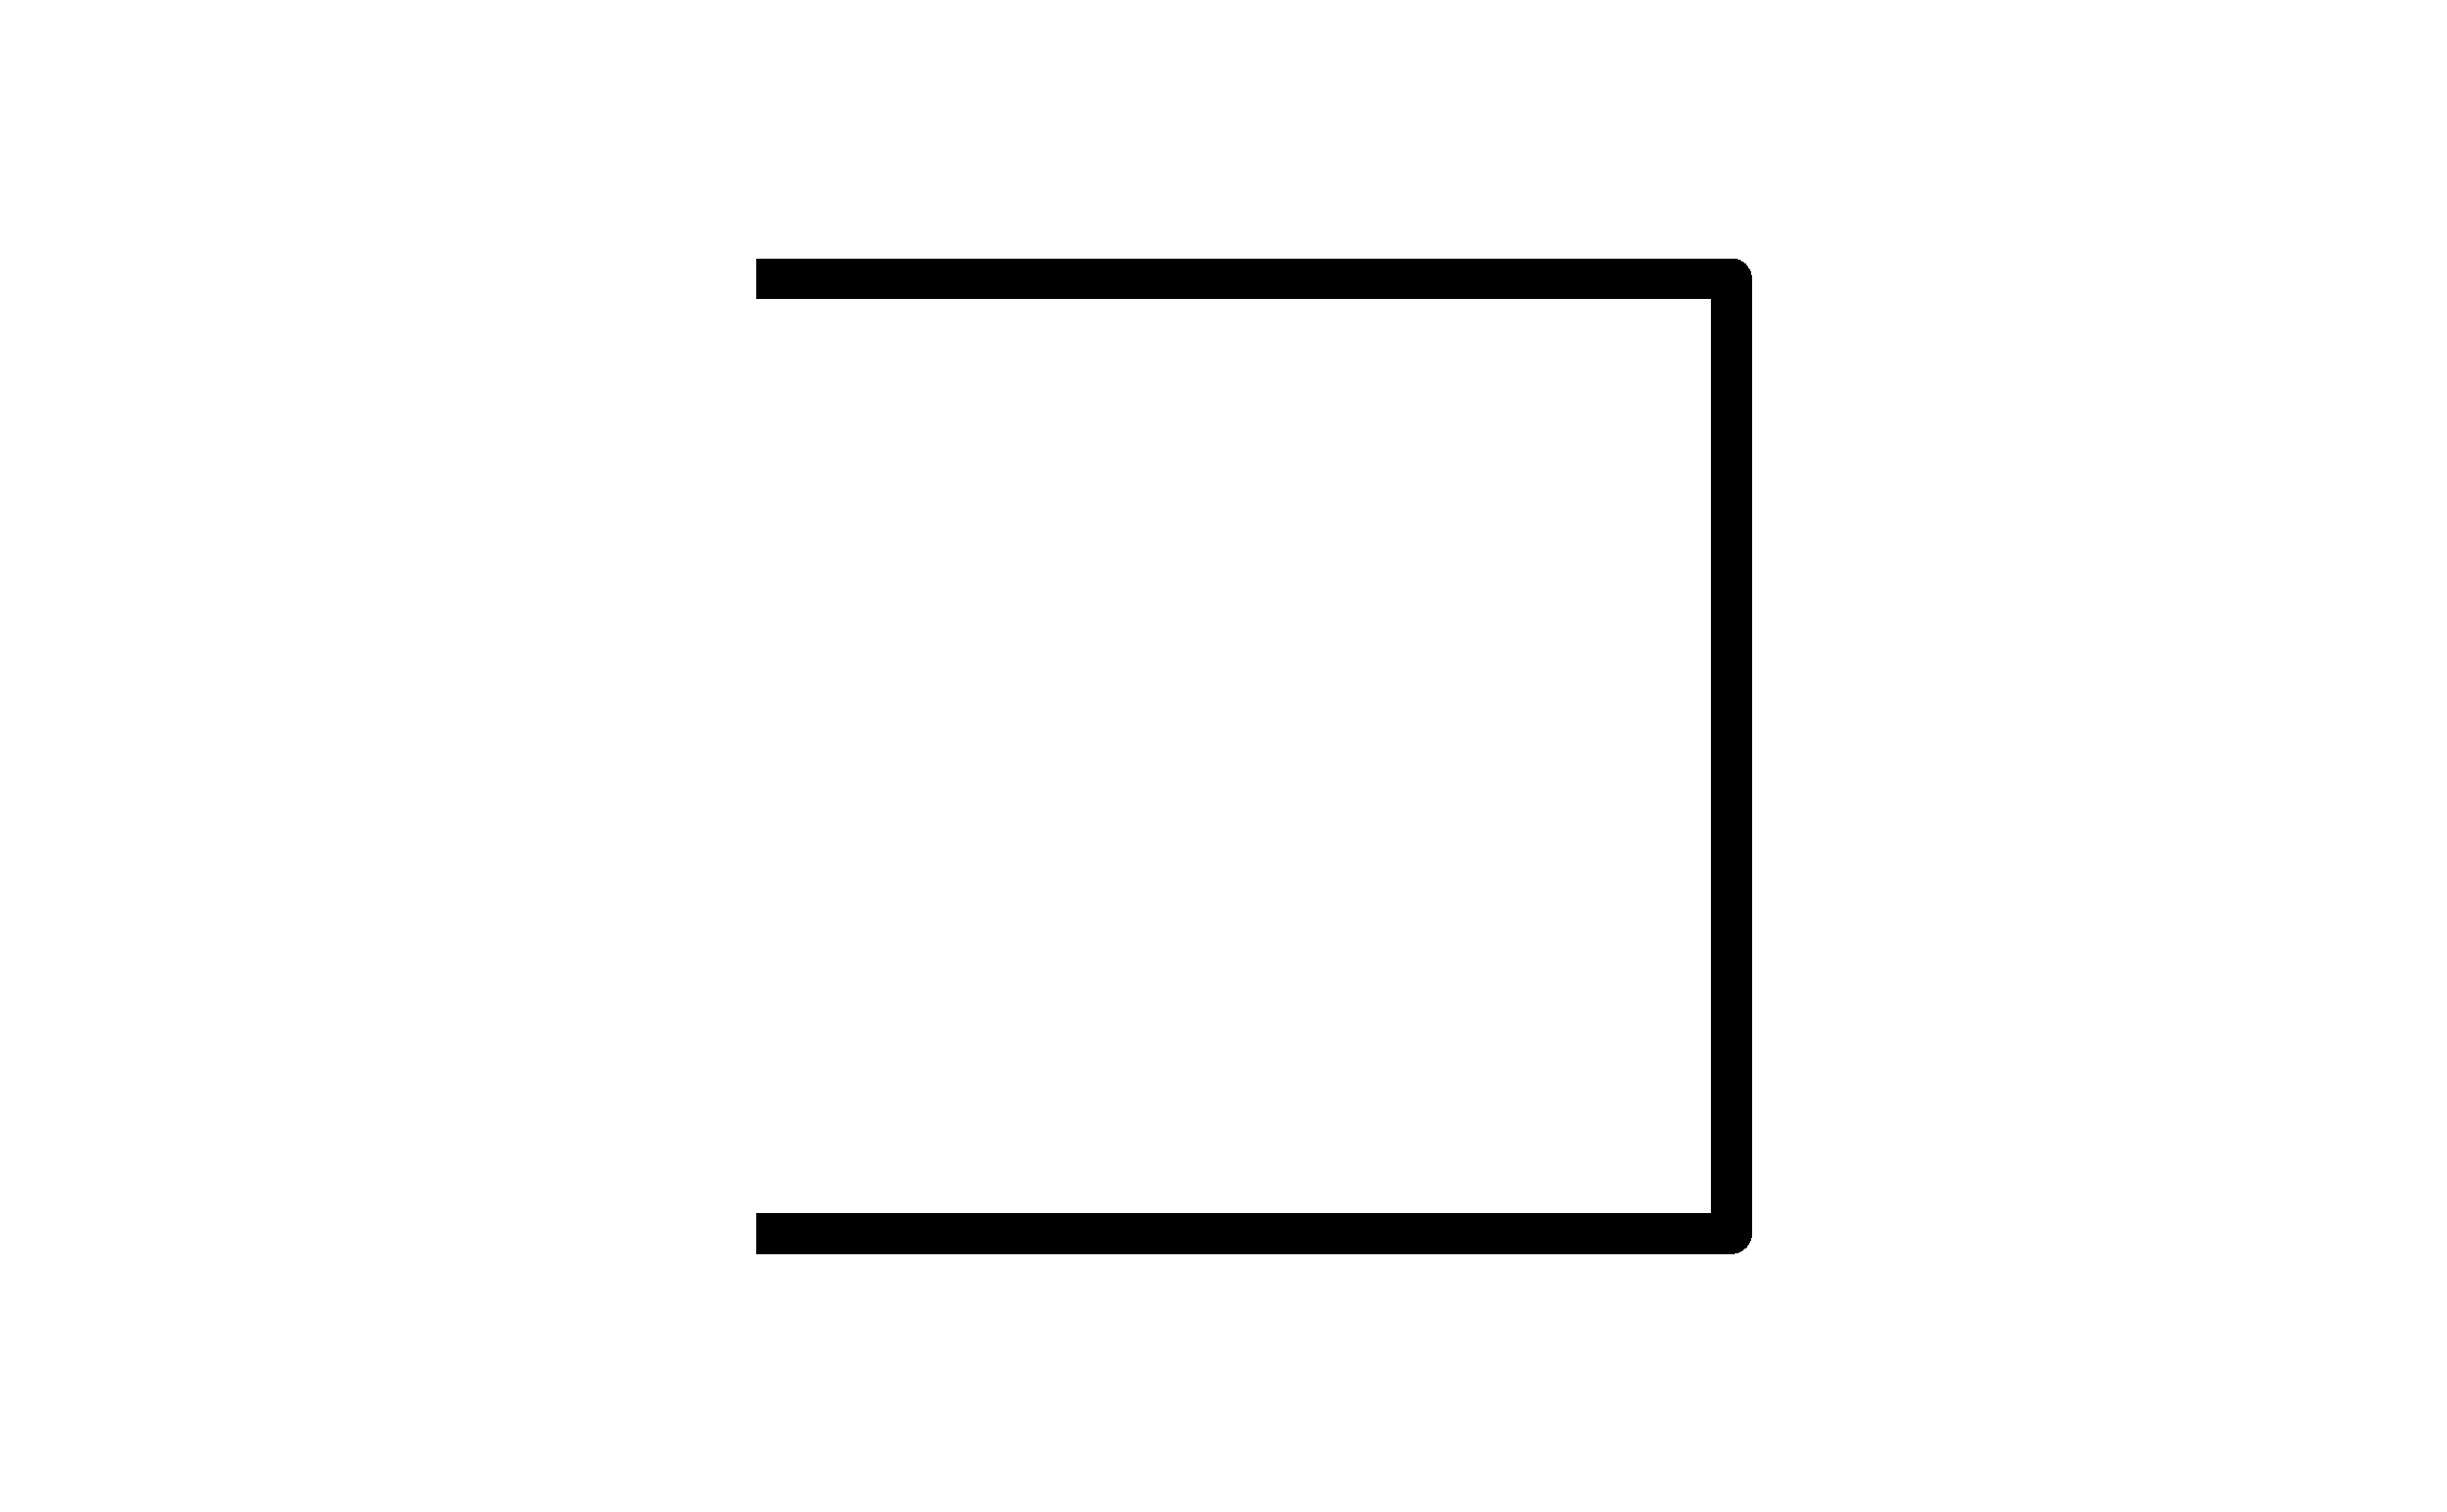
\includegraphics[width=1.5 cm]{supplement/beta_cluster_example_2/pictures/21/state_cluster_shapes_150.pdf} 
    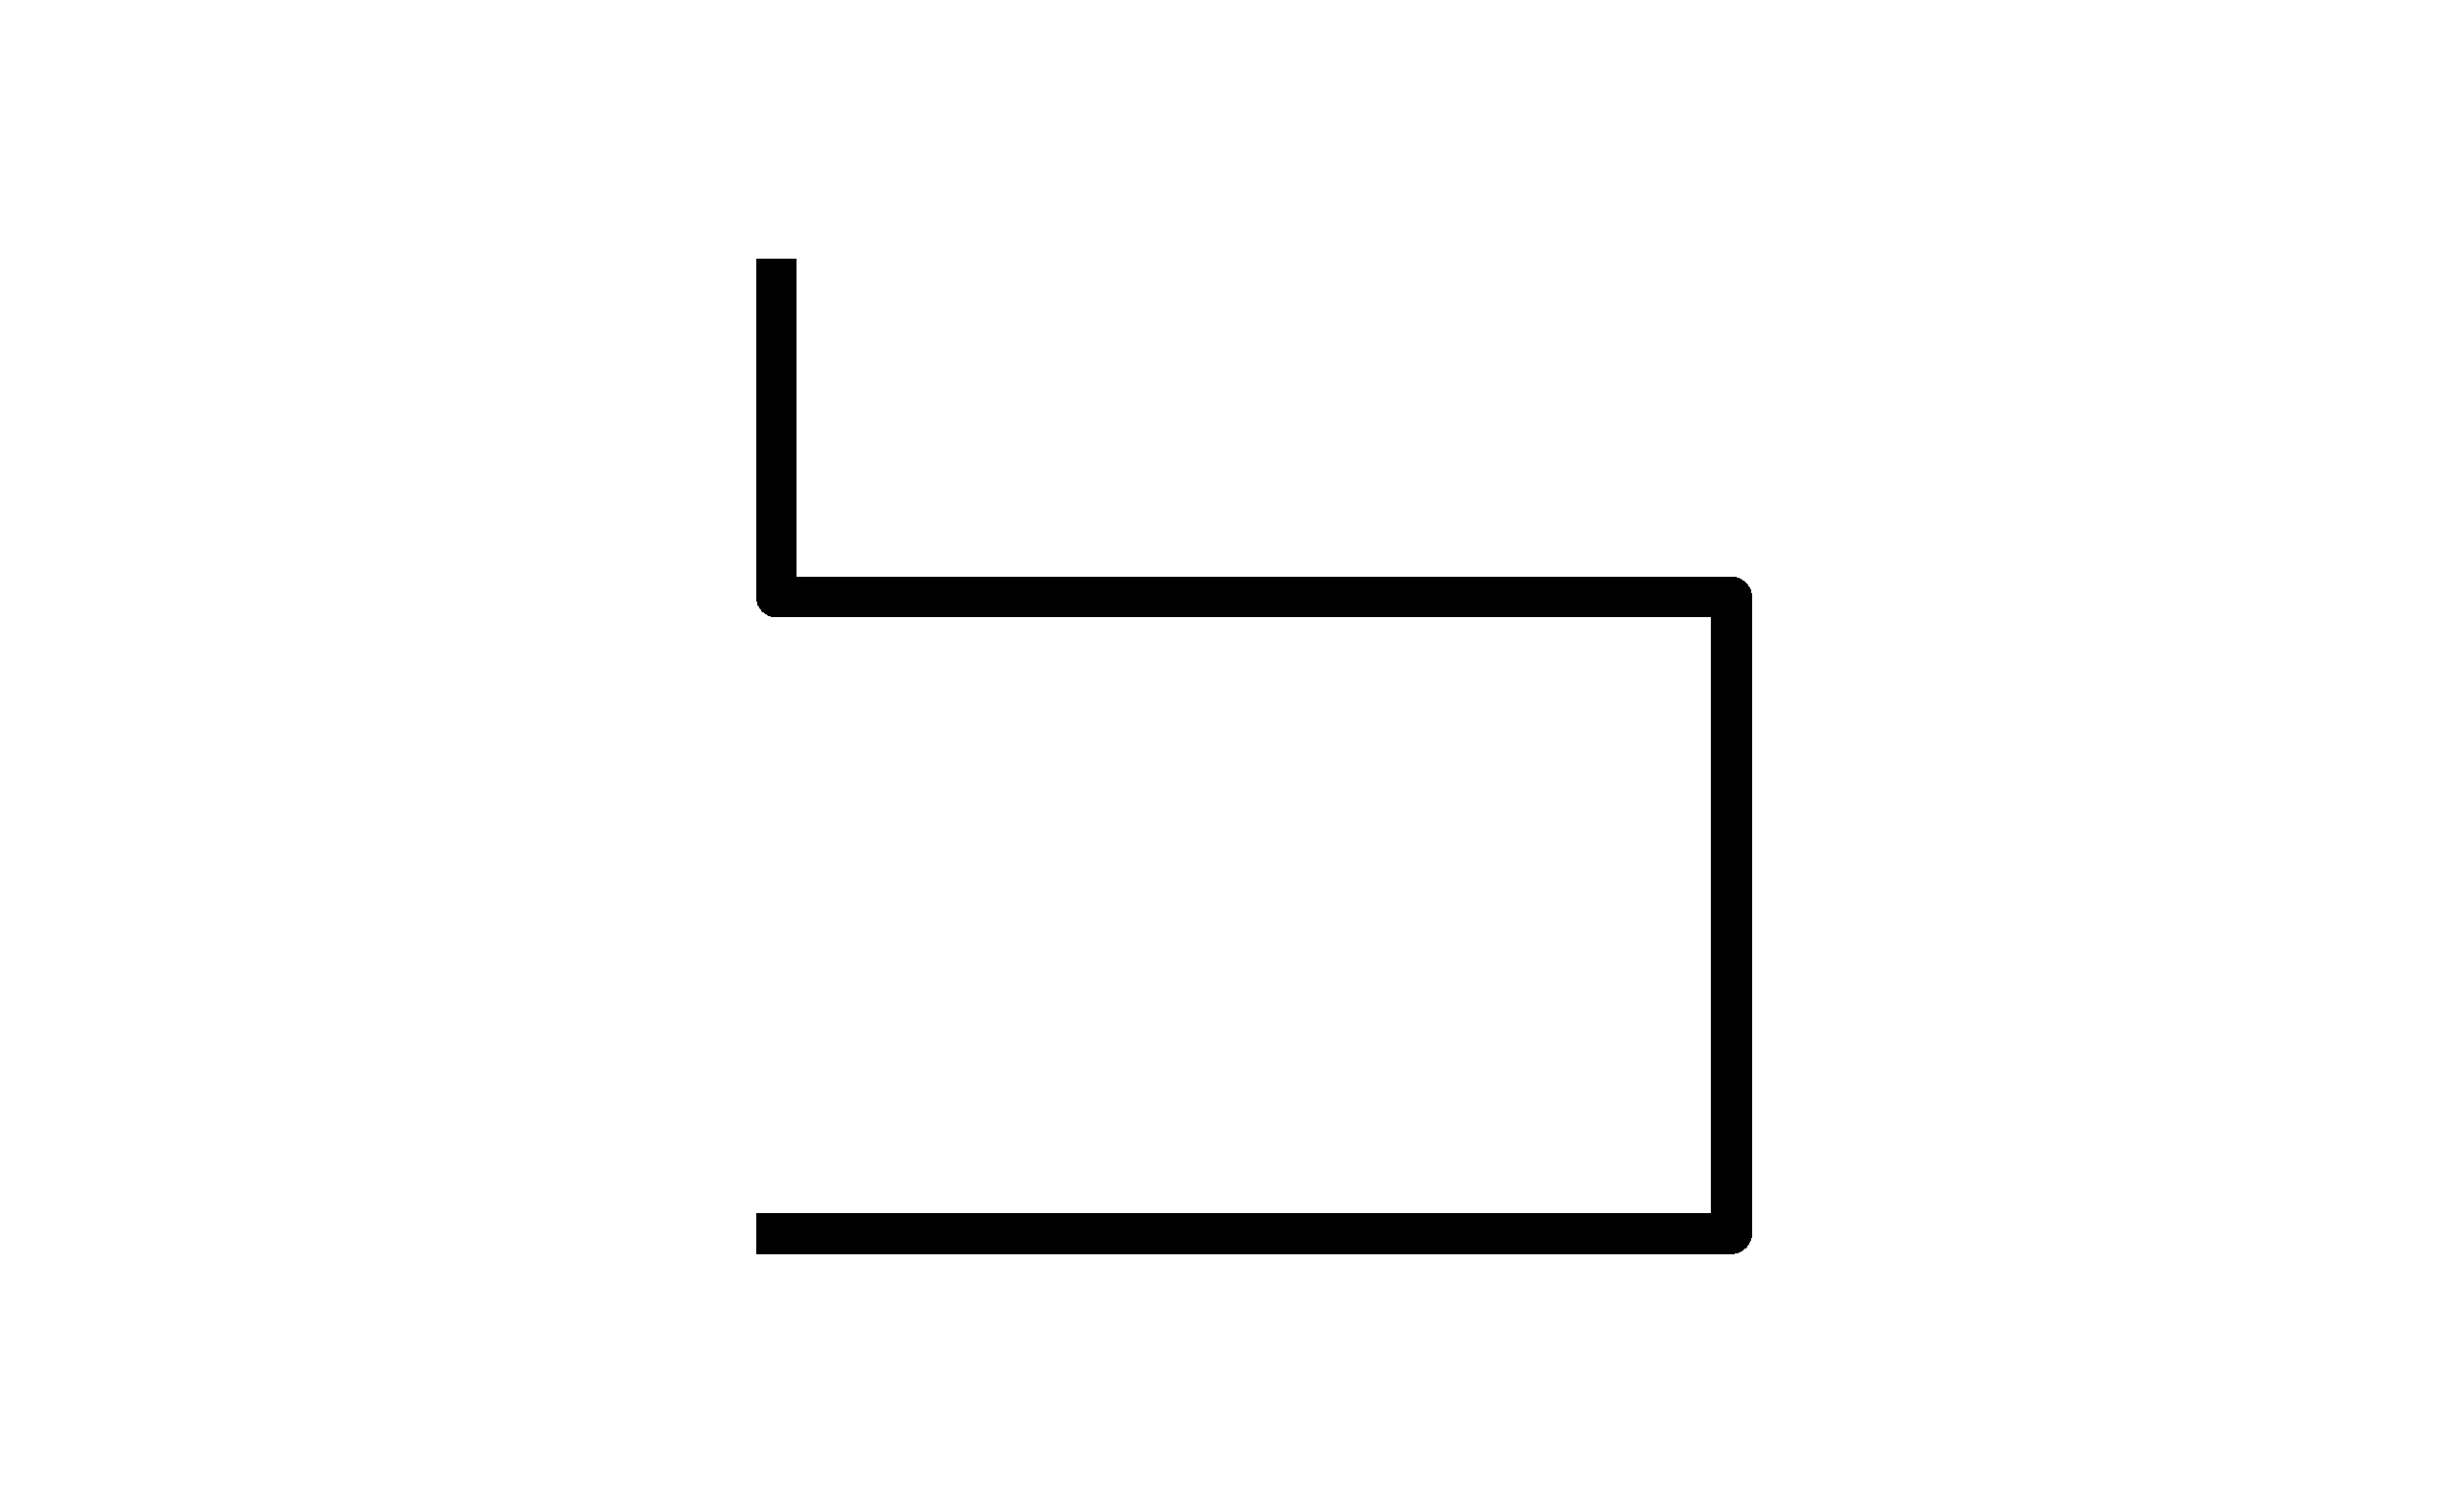
\includegraphics[width=1.5 cm]{supplement/beta_cluster_example_2/pictures/21/state_cluster_shapes_17.pdf} \\
    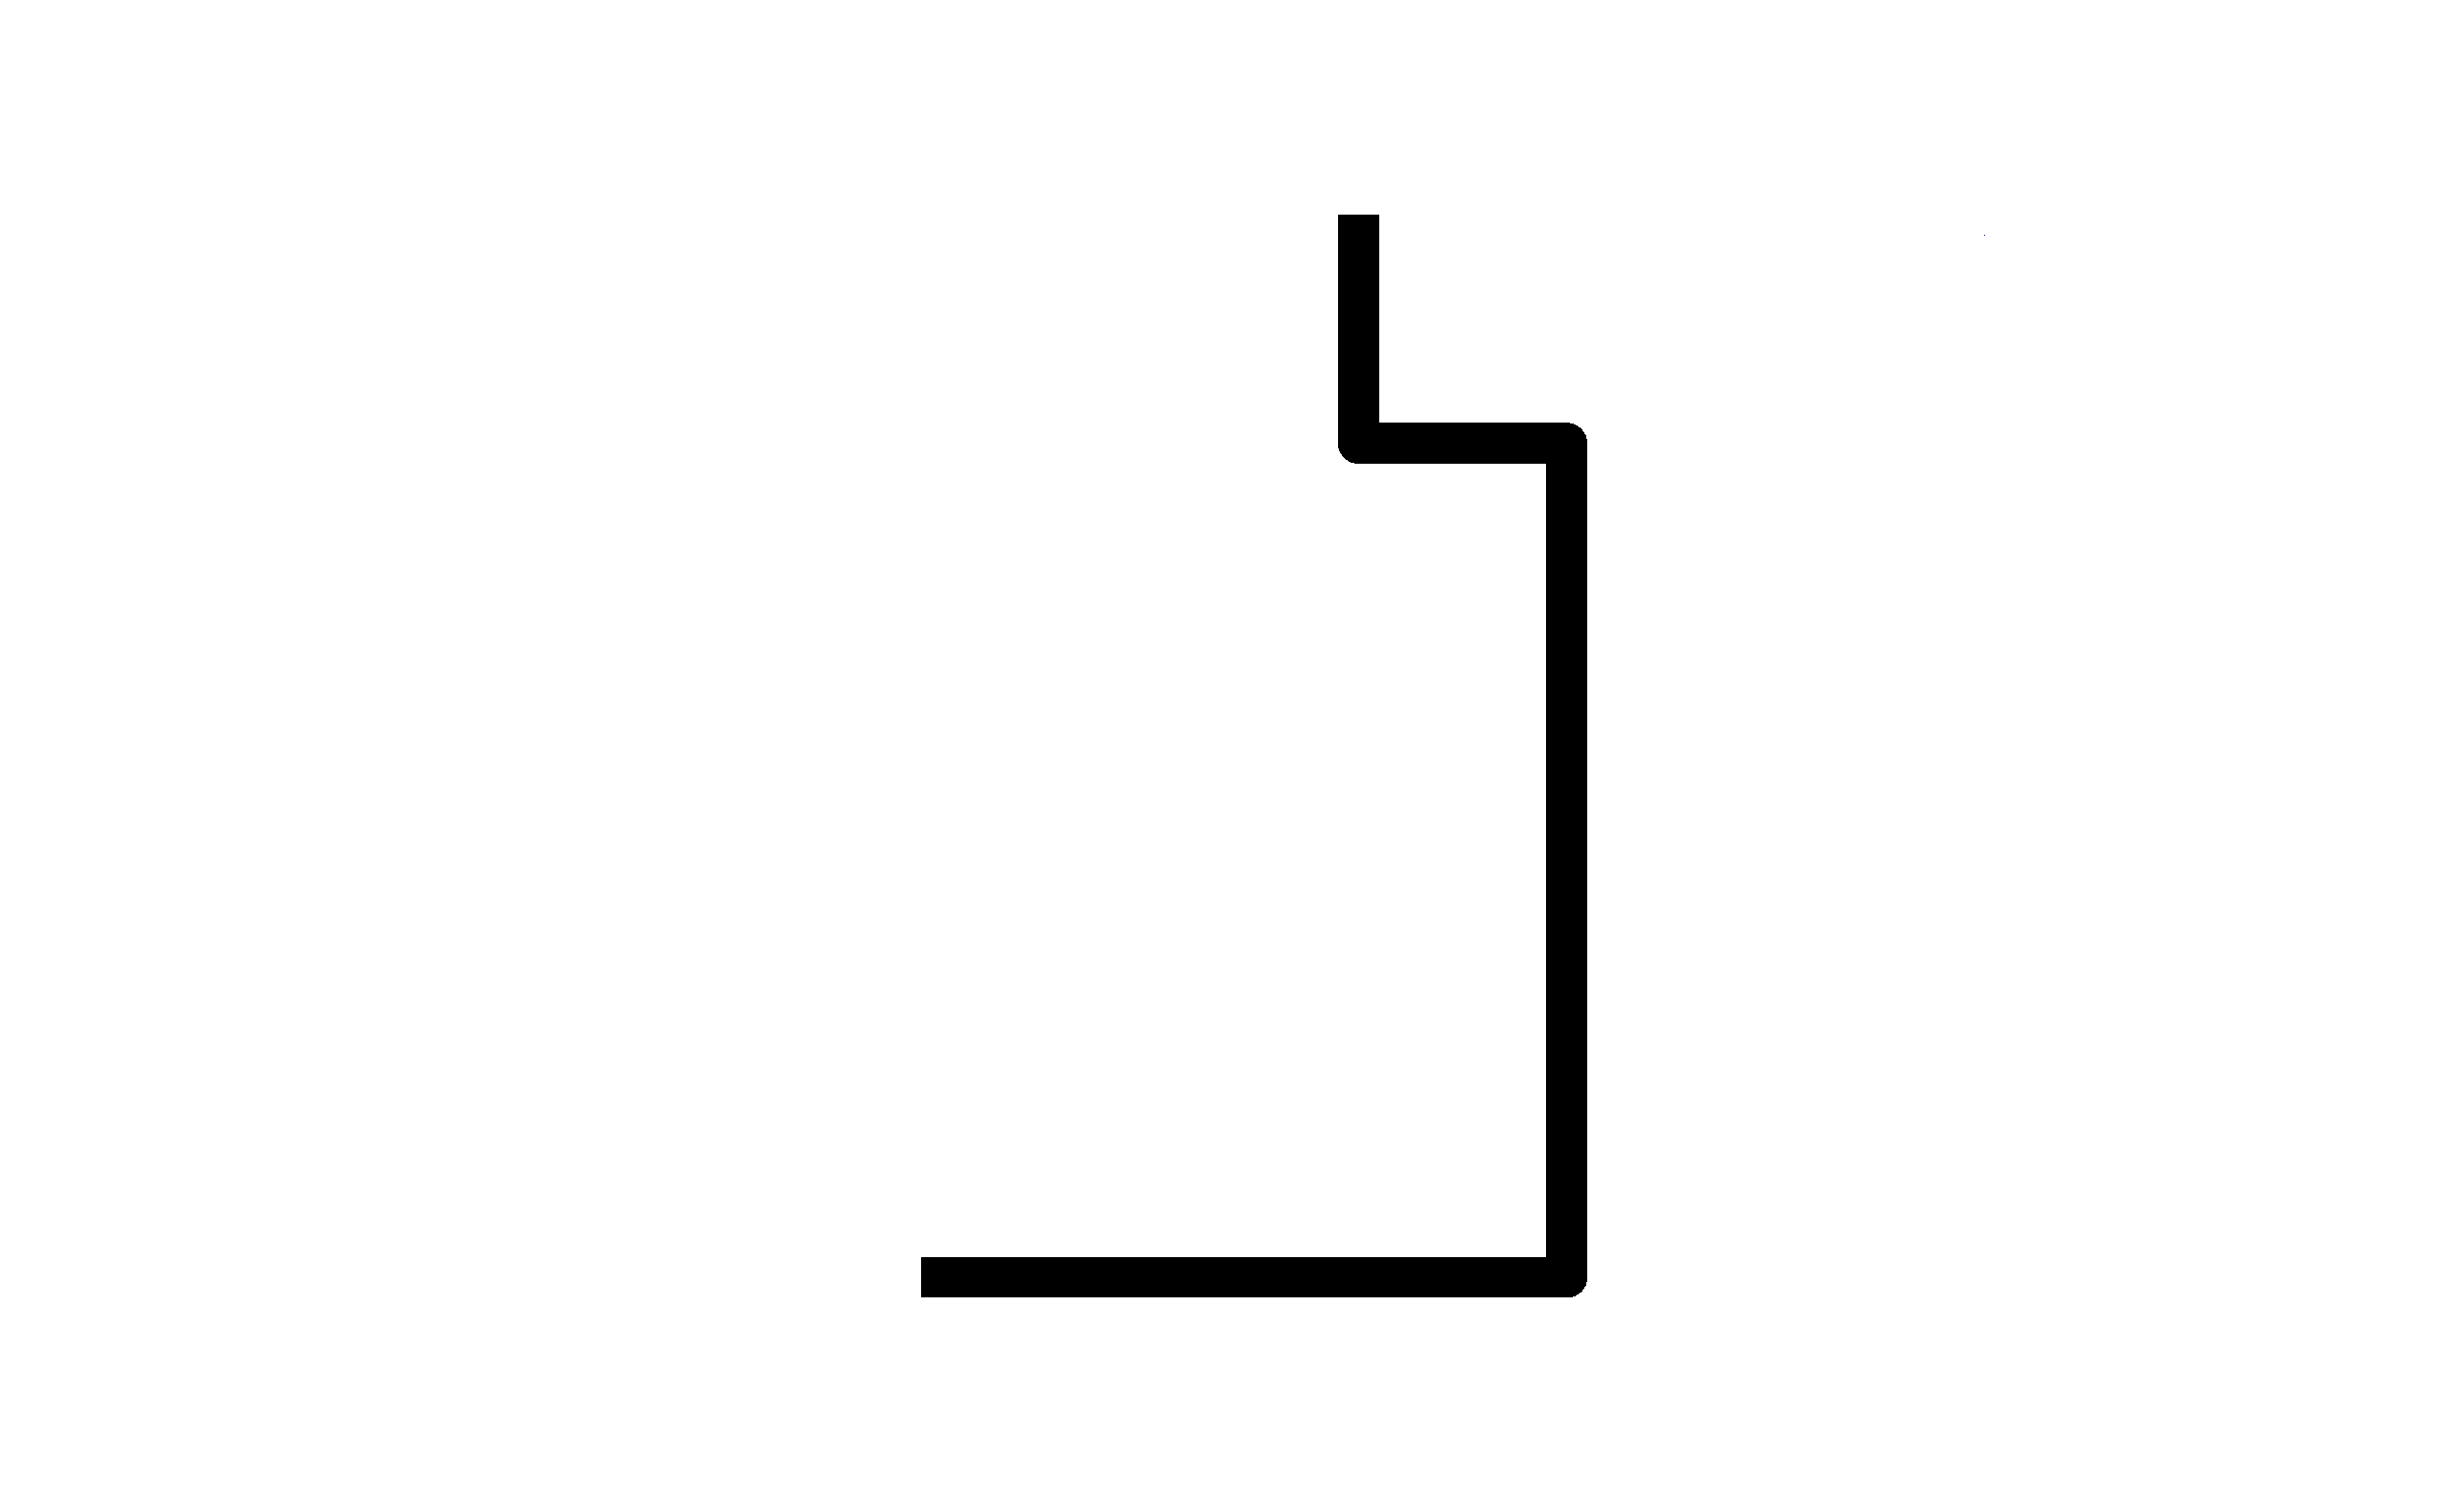
\includegraphics[width=1.5 cm]{supplement/beta_cluster_example_2/pictures/21/state_cluster_shapes_32.pdf} 
    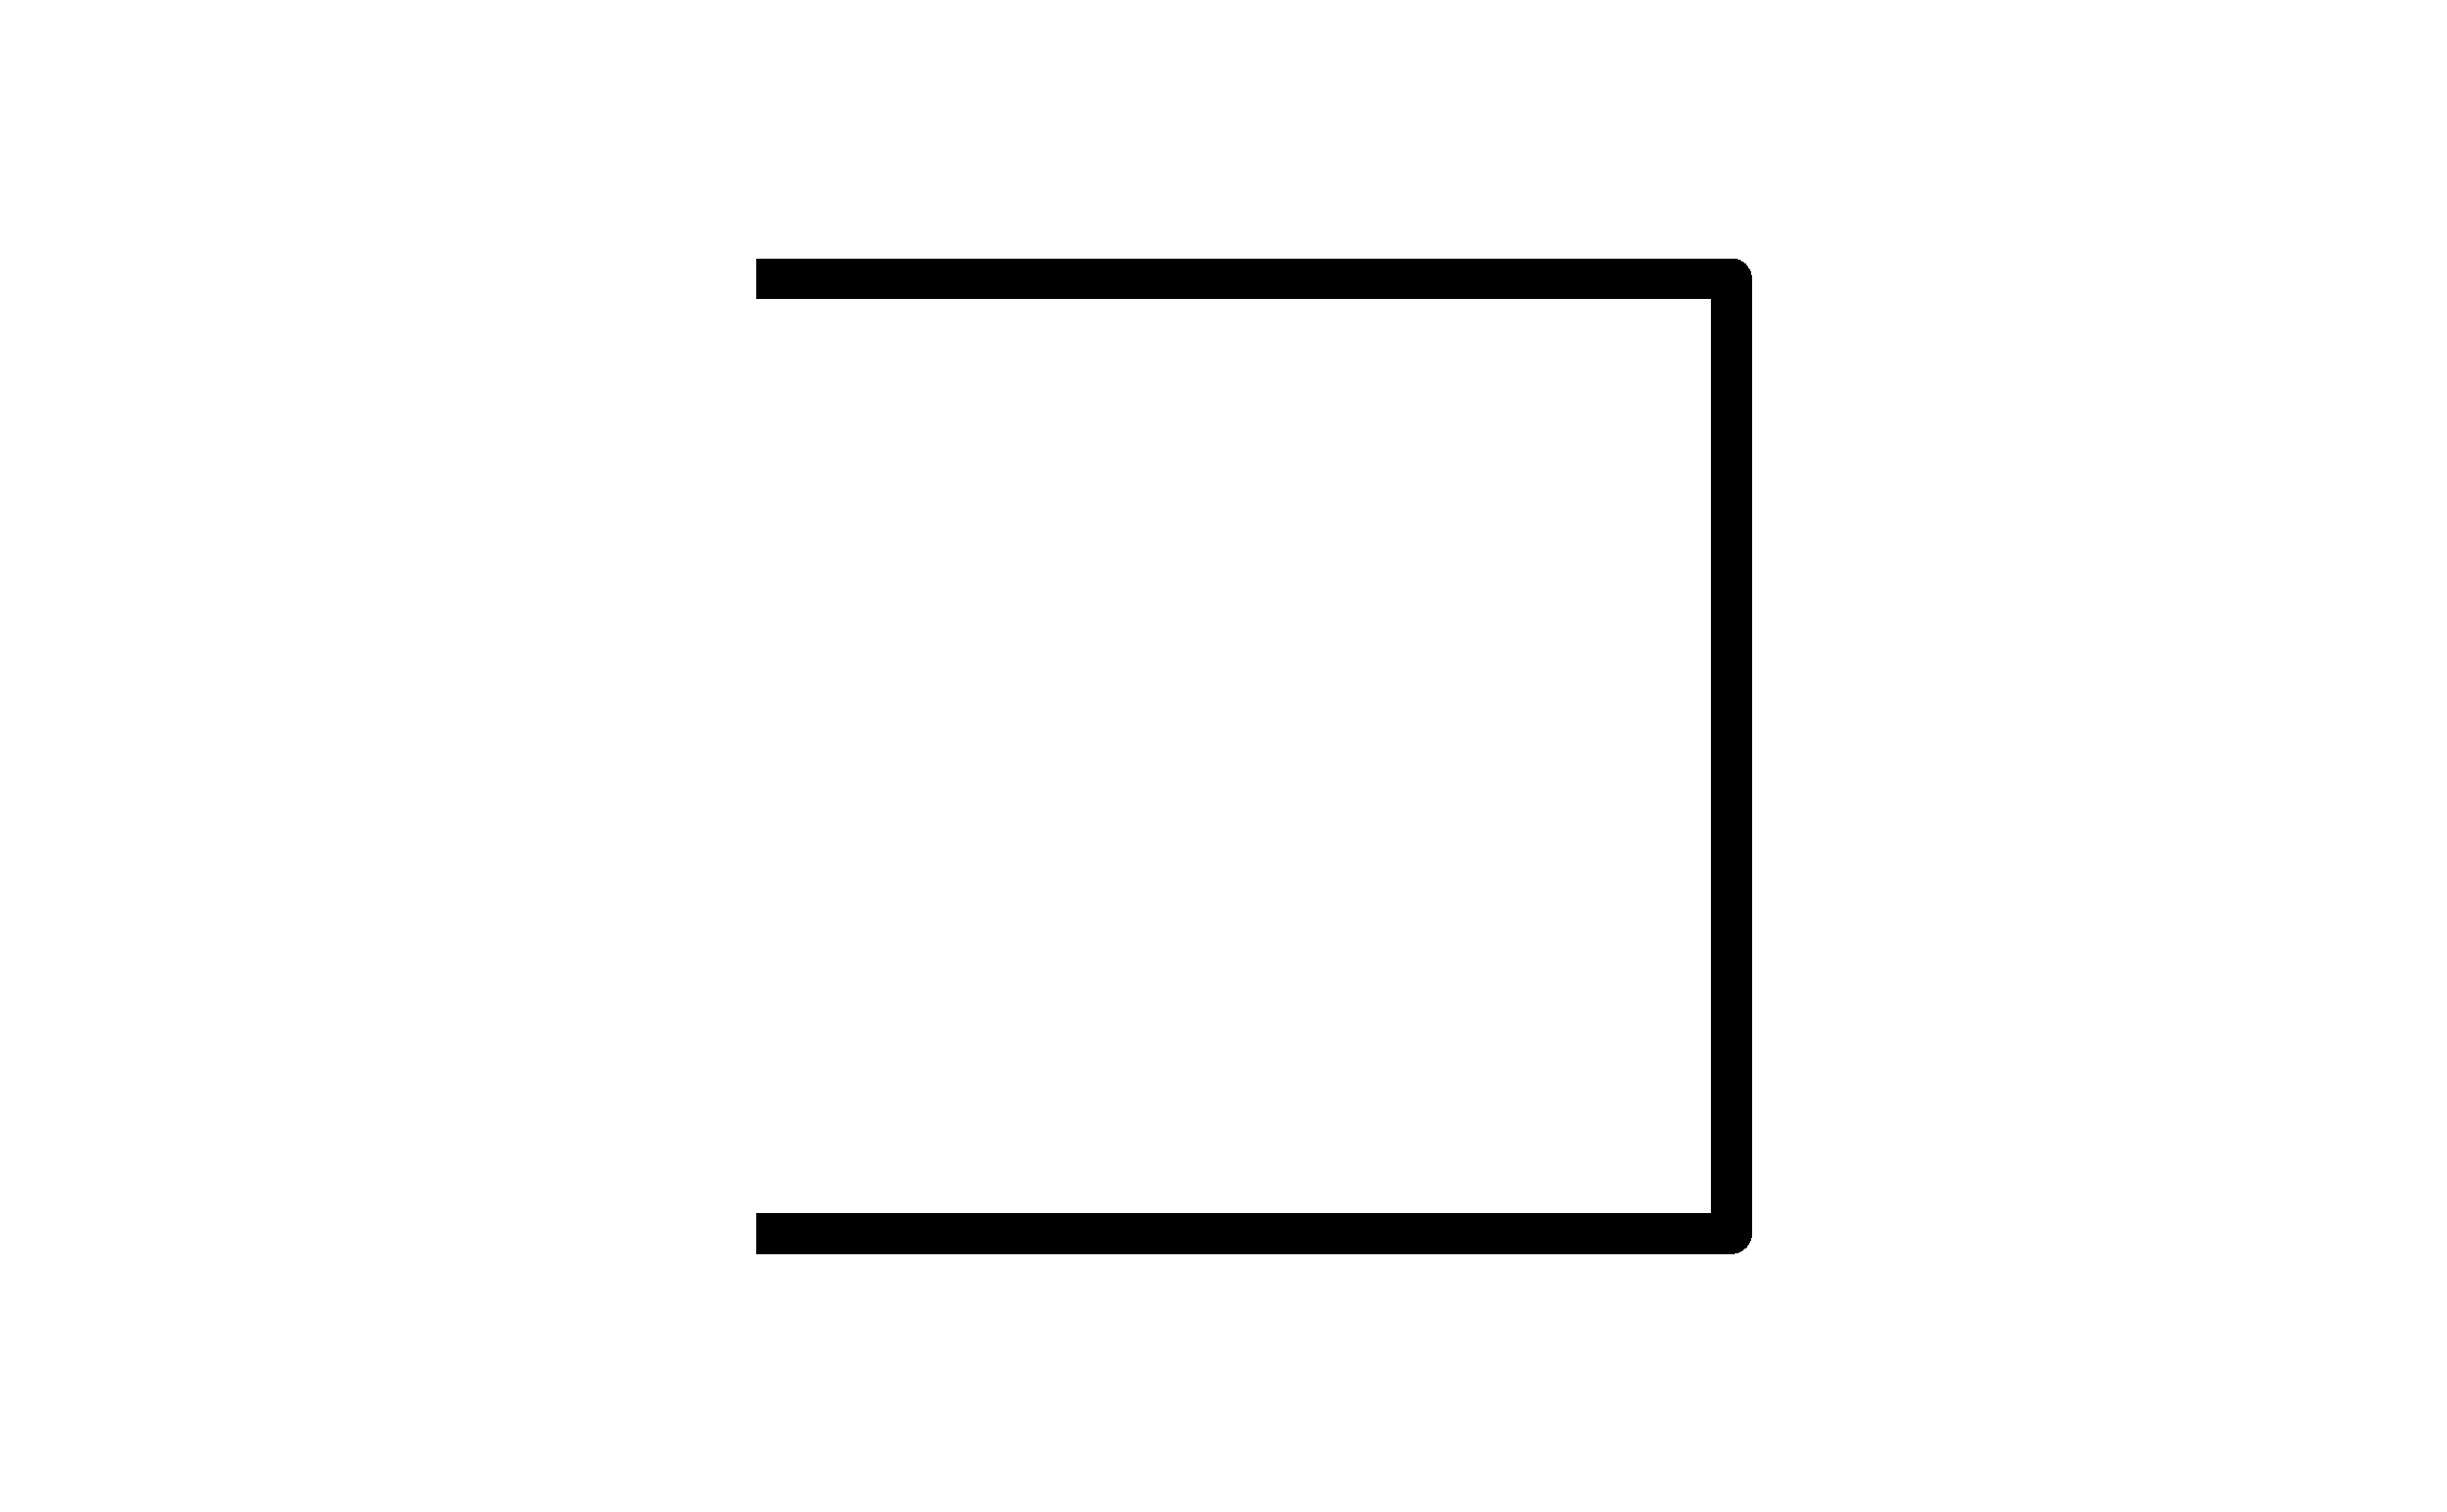
\includegraphics[width=1.5 cm]{supplement/beta_cluster_example_2/pictures/21/state_cluster_shapes_200.pdf} \\
  	 $c_\chem{R}$ random coil
    \end{minipage}
    };
    \node[macrostate_vertex] (I) at (1.5*\vertexshiftamount,0)   {
    \begin{minipage}{3.1cm} \centering
    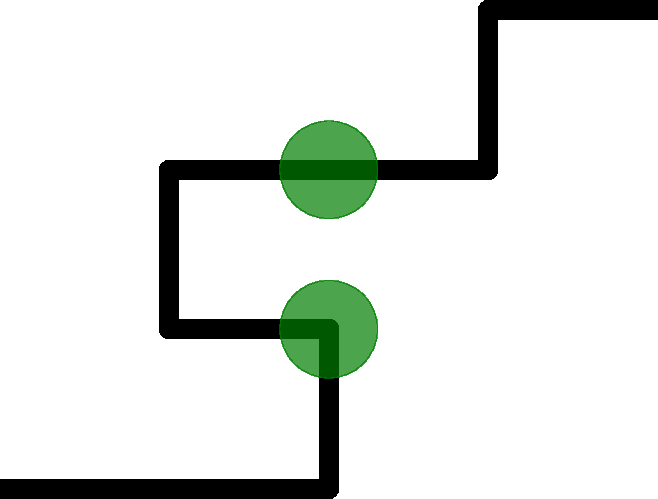
\includegraphics[width=2 cm]{supplement/beta_cluster_example_2/pictures/saved_macrostates/intermed.png} \\
  	 $c_\chem{I}$ intermediate \\ (turn formation)
    \end{minipage}
	 };
    \node[macrostate_vertex] (F) at (3*\vertexshiftamount,0)   
    {
    \begin{minipage}{3.1cm} \centering
    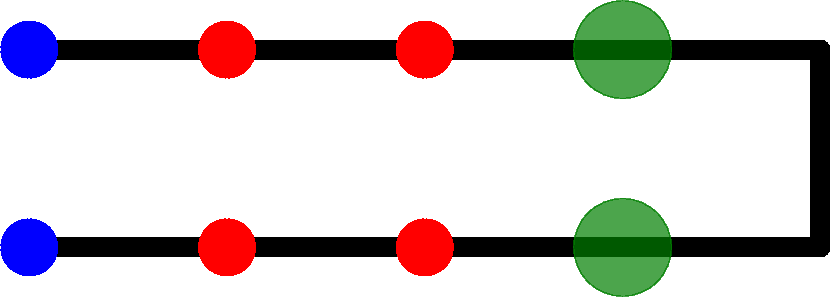
\includegraphics[width=2.5 cm]{supplement/beta_cluster_example_2/pictures/saved_macrostates/native.png} \\
  	 $c_\chem{F}$ native state
    \end{minipage}
    };

  \tikzstyle{EdgeStyle}=[bend right]
  \Edge[label=$\B{S}_{\chem{R I}}$](R)(I)
  \Edge[label=$\B{S}_{\chem{I R}}$](I)(R)
  
  \tikzstyle{EdgeStyle}=[]
  \Edge[label=$\B{S}_{\chem{I F}}$](I)(F)
  
\end{tikzpicture}
}


%\end{comment}


\begin{document}

\suppressfooter
\begin{preamble}

\iffinal{}{\newpage}
\begin{DUTdedications}
%
\vspace*{\fill}
%
\begin{center}
\setstretch{2}
\begin{minipage}{8 cm}
\begin{center}
\hrulefill\\
This thesis is dedicated to Cara Hoppe.\\ 
I respect her as my peer,\\
and cherish her as my wife.\\
Her love and support made this work possible. \\
%\hrulefill\hspace{0.2cm} \leafNE \hspace{0.2cm} \hrulefill
\hrulefill
\vspace{6em}
\end{center}
\end{minipage}
\end{center} 
%
\vspace*{\fill}
%
\end{DUTdedications} 
\iffinal{}{\newpage}

\begin{acknowledgments}
  \iffinal{}{\setstretch{1.5}}
The completion of this thesis could not have been done without the tireless support of my advisor, Dr. Jian-Min Yuan. I am deeply indebted for the support he has provided over the years. As a mentor, he helped me develop my skills as a scientist and honed my critical thinking. He is an endless source of new ideas and has taught me how to effectively communicate in the scientific world. 

I would also like to thank the physics department at Drexel for helping me prepare for the journey ahead. In particular, both Dr. Michel Vallieres and Dr. Robert Gilmore have been gracious enough to spend many afternoons discussing every interesting theory I've come across. Their insights and enthusiasm for physics and mathematics is inspiring. 

I would like to thank my family, my wife, Cara Hoppe, and my children, Hazel and Jackson Hoppe. They cheerfully remind me of the world outside and always bring a smile to my face. Finally, I would like to thank my uncle, Fred Stein, who introduced me to physics and all its wonders at an early age.
 
  \end{acknowledgments}
  \iffinal{}{\newpage}

  \listoffigures 
  \iffinal{}{\newpage}

  \tableofcontents 
  \iffinal{}{\newpage}

  \begin{abstract}
  \iffinal{}{\setstretch{1.5}}
  \setstretch{1.5}
A protein's ultimate function and activity is determined by the unique three-dimensional structure taken by the folding process. Protein malfunction due to misfolding is the culprit of many clinical disorders, such as abnormal protein aggregations. This leads to neurodegenerative disorders like Huntington's and Alzheimer's disease. We focus on a subset of the folding problem, exploring the role and effects of entropy on the process of protein folding. Four major concepts and models are developed and each pertains to a specific aspect of the folding process: entropic forces, conformational states under crowding, aggregation, and macrostate kinetics from microstate trajectories. 

The exclusive focus on entropy is well-suited for crowding studies, as many interactions are non-specific. We show how a stabilizing entropic force can arise purely from the motion of crowders in solution. In addition we are able to make a a quantitative prediction of the crowding effect with an implicit crowding approximation using an aspherical scaled-particle theory.

In order to investigate the effects of aggregation, we derive a new operator expansion method to solve the Ising/Potts model with external fields over an arbitrary graph. Here the external fields are representative of the entropic forces. We show that this method reduces the problem of calculating the partition function to the solution of recursion relations. 

Many of the methods employed are coarse-grained approximations. As such, it is useful to have a viable method for extracting macrostate information from time series data. We develop a method to cluster the microstates into physically meaningful macrostates by grouping similar relaxation times from a transition matrix.  

Overall, the studied topics allow us to understand deeper the complicated process involving proteins.
  \end{abstract} 

	\iffinal{}{\newpage}

\end{preamble}


\begin{thesis}
  \pdfbookmark[-1]{Main Matter}{Main Matter}
  %\setstretch{1.2}
  \chapter*{Preface}

\begin{comment}
  Throughout history, scientific fields have split, merged and been made obsolete. What we find important is dictated by our philosophical ideals, economic status, cultural norms and scientific curiosity. The current frontiers of science aim probe our understandings of the very laws of physics through our studies of the exotic Higgs boson to recreating the wistful alchemical dream of artificial atoms through quantum dots. Corporeally, we have staked out the biological form as new fertile ground for us explore and pioneer. The explosive growth in this interest, fueled by new technologies, has lead to the growth of a new multi-disciplined approach called biophysics.
\end{comment}

Traditionally, the components of biophysics, biology and physics, have a tangential mode of thought.  Biology, the study of living things, is a field governed by qualitative observation and later mathematical models are applied. Prediction comes from the understanding of the various mechanisms that are often intricately coupled. On the other hand, a mature branch of physics is governed by the mathematical form first. Ideas are founded from first principles, from which the physical laws are then derived. If these predictions fail to accurately portray reality the fundamental assumptions are discarded and presumed to be false. The successful theories in physics have a far greater precision than the biological counterparts. How then do the two fields reconcile, the dogma of each being so different?
%
\begin{equation*}
  \chem{bioPHYSICS \longleftrightarrow BIOphysics}
\end{equation*}

In this author’s opinion, the field of biophysics has truly made possible by a third kind of science. After experiment and theory comes modeling, an approach that has been greatly enhanced by the use of modern day computers. Scientific modeling incorporates rigorous mathematical derivations, yet the results are interpreted as though they were experimental evidence. It is rapidly being recognized as an important and vital component to our scientific endeavors.\cite{reed_computational_2005} In some ways modeling takes the best of both forms, allowing each to contribute. This approach has been used in many diverse fields such as meteorology, economics, and our present topic, biophysics.

Biophysics has an implicit scale. Usually the scale spans from collections of cells (on order of microns) to collections of atoms (on order of angstroms). As an example of the types of objects currently studied, Figure \ref{fig:conf_words} shows the usage of the words found in abstracts of presentations and posters at a recent biophysics conference. The three dominant objects that were studied were proteins, cells, and membranes. The larger structures (except in the cases of aggregation) traditionally studied in biology are out of the scope of most biophysical studies. 
%
\begin{figure}
  \begin{centering}
    \fbox{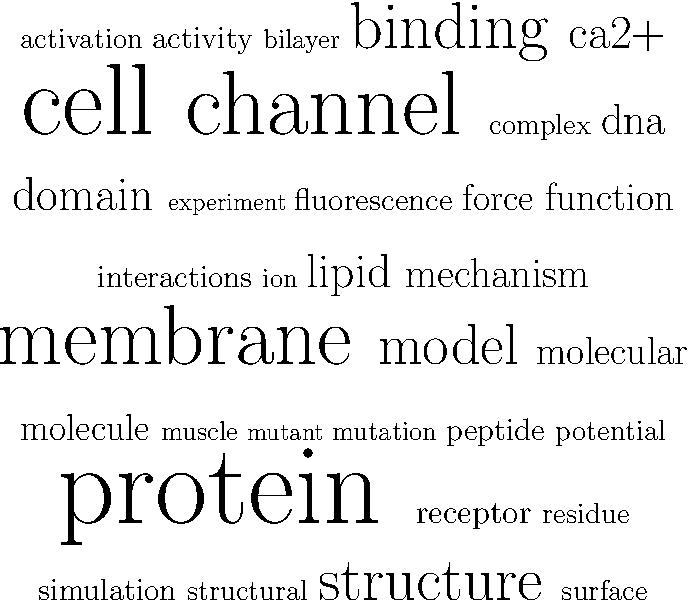
\includegraphics[height=5 cm]
      {pictures/wordcloud_conf/abstract_wordcloud.pdf}}
    \caption{Snapshot of the most commonly used words in the abstracts of the 2010 Biophysical Conference in San Francisco.\cite{BPS_conf_2010} Larger words correspond to a greater usage. Note that the prominent words, protein, cell, and membrane set the length scale that narrows the focus of the discipline.}
    \label{fig:conf_words}
  \end{centering}
\end{figure}

As we move to smaller structures we find ourselves in the realm of quantum chemistry and pure physics. In this regime, theories of ``first-principle'' abound. That is, starting from a set of empirically verified postulates, equations are derived which predict the dynamics and structure of the system. As we move to larger structures we are back in the traditional biological realm, where the role of classification dictates the functionality. 
For the theoretical and modeling based biophysicist the aim is to derive from first-principle equations. The attempt is to classify and organize the higher-order structures found at this scale. The predictions must ultimately be vetted by experiment studies, thus neither group can work in isolation.
%The approach of a biophysicist, due to its multi-disciplined nature, often depends on the formal training of the scientist conducting the experiment. Pure observationalists and theorists exist, often coming from their respective fields, but their appearance is the exception rather than the rule. Sampling from the abstracts of a recent meeting of the Biophysical Societies 2010 Annual Meeting \cite{BPS_conf_2010}, the largest in it's field with a few thousand talks, symposia and poster presentation, one finds that many scientists are engaged in the modeling approach, from the development to the interpretation. 

It is here that we begin our discussion, at the crossroads of two diverse fields whose singular aim is no less than the understanding of the phenomena behind life itself.


  \restorefooter

  %CHAPTER: Introduction
  \chapter{Introduction}
\vspace{-1em}
\epigraph{
  \textit{In the drama of life on a molecular scale, proteins are where the action is.}
}{Lesk\cite{lesk_introduction_2001}}
%
In contrast to other important biological molecules, proteins have a remarkable diversity of spatial structures and thus a wide variety of biological functions. Some of the many complex tasks proteins can perform include the ability to\cite{lodish_molecular_2004, echenique_introduction_2007}
\begin{itemize}
\item interpret inter-cellular signals such as insulin \& EGF in signaling pathways\cite{ghosh2006simulation, miller2007systems}
\item transport other species\cite{zakharov2009microrheological}
\item govern chemical conversion
\item control gene expression
\item convert chemical energy into mechanical energy
\item serve as building blocks to biological structures (\ie collagen and virus coats) and,
\item act as chaperones to help other biological agents function (such as GroEL in bacteria).
\end{itemize}
As such, the study of proteins, either directly or indirectly, encompasses the core of many microbiological studies. A protein's ultimate function and activity is determined by a process called folding. This folding process guides the protein into a specific three-dimensional form. Unsurprisingly, protein malfunction due to misfolding is the culprit of many clinical disorders, from cancers to abnormal protein aggregations (leading to neurodegenerative disorders like Huntington and Alzheimer\cite{uversky_intrinsic_2009}).

The study of proteins is paramount to the understanding of life itself. In this thesis we attempt to elucidate some of the properties associated with the folding process. We present a detailed study of the conformational states under various conditions.

\section{Protein Structure}

A protein can be broken down into a hierarchy of structures, each with a different set of motifs describing it. A protein is a polymer linking together a series of amino acids. Like DNA, a protein is composed of a simple alphabet of twenty naturally occurring amino acids (whereas DNA has a four-letter alphabet of base pairs). These amino acids are connected along a backbone of carbon, nitrogen and oxygen atoms. A protein has a primary structure enumerated by the ordered sequence of these letters. These encodings, along with the physiological conditions, uniquely determine the structure of the protein and hence its ultimate function. 

Amino acids connected along the backbone cannot assume arbitrary angles with respect to each other.  This stereochemistry is vividly displayed on Ramachandran plots.\cite{ramachandran_stereochemistry_1963} These plots typically illustrate the dihedral (or $\phi$-$\psi$) angles that are allowed due to energetic considerations. This is just one type of the forces which guide the folding process. 

At this structural level, certain motifs are seen more often than others. The most frequent structures common to proteins are the $\alpha$-helices and the $\beta$-strands. At this level of hierarchical complexity, the motifs are called the secondary structure. At the next level up, the tertiary structure involves the arrangement of the secondary-structure elements, helix bundles, and $\beta$-sheets. These are in turn coalesced into even larger quaternary structures for proteins with multi-domains.

The secondary structures are a good starting point for the study of the protein. In the absence of stabilizing interactions, the protein will be unfolded in a so-called random-coil structure. When hydrogen bonds form between residues along the backbone, the protein will form well-defined (locally periodic) structures of $\beta$-sheets and $\alpha$-helices. Hydrogen-bonds, hydrophobic interactions, van der Walls and electrostatic interactions all contribute to the folded structure of a protein.

\subsubsection{Secondary Structures: 
  \texorpdfstring{$\alpha$}{Alpha}-helices and 
  \texorpdfstring{$\beta$}{Beta}-sheets 
}

The first of the secondary structures, the $\alpha$-helix, is stabilized by hydrogen bonds between the \chem{CO} and \chem{HN} groups of the backbone four residues down the chain. In theory, there are multiple ways a helix could be formed: both right-handed, left-handed and different `tightness' of the helix. Almost all of these other conformations except for the $\alpha$-helix are energetically unfavorable and are rarely observed in real proteins. In an $\alpha$-helix all the hydrogen-bonds are made by neighbors that are close along the chain, thus the stabilizing forces involved are often referred to as short-range. These helices are formed very rapidly, on the order of tenths of $\mu s$. There are approximately 3.6 residues per helical turn, which from a modeling standpoint, presents a problem if the protein is coarse-grained onto a lattice that can not accommodate the exact structure.

The $\beta$-sheet is a lateral packing of $\beta$-strands; each strand is a short extended peptide segment. Just like the $\alpha$-helix, a $\beta$-sheet can exist in several different forms, however these other forms are actually found in real proteins. The two main distinctions are parallel and anti-parallel $\beta$-sheets. The interactions between the $\beta$-stands act over short distances but can be far apart along the length of the chain; they are often referred to as long(er)-range forces when compared to the $\alpha$-helix. Again, in contrast to $\alpha$-helices, $\beta$-sheets  have a wide variability in folding times. Some shorter peptide sequences can form as quickly as $0.5\mu s$, while others can take hours!\cite{xu_probing_2008} 

\section{Protein folding}
Since Anfinsen's discovery in the early 1960's that a denatured protein can spontaneously self-assemble when denaturants are removed,\cite{anfinsen_kinetics_1961} researchers have attempted to deduce which mechanisms and pathways are important to the folding process. One of the main challenges of the field is to predict the final native structure from the primary structure. To put it mildly, this has not been an easy task. Not only does a peptide (small protein) contain hundreds of atoms, it resides in a water based solvent where the effects are mediated out at lengths of several molecules away. A typical molecular dynamics simulation contains thousands of atoms making a full scale quantum computation impossible by today’s standards. Classical kinetic approximations are possible, yet consume thousands of hours of computing time for a single trajectory. This is tantamount to a limited observational study; predictions of statistical quantities such as specific heat can only be crudely estimated. These molecular dynamics simulations are, however, the best method for studying dynamics of the system without the need for costly experiments. The mechanism in which protein folding occurs can often be determined out of such \textit{in silico} experiments. 

Backing up the veracity of the computational molecular experiments are the physical experiments themselves. The traditional methods of studying an unknown sample such as mass spectrometry, lacked the resolution needed when dealing with complexities of proteins. The more detailed studies of protein structure came from advances in experimental instrumentation. These experimental techniques were sometimes adapted from other fields, but often were invented for the study of biological molecules. X-ray crystallography was created to study the periodic arrangements in crystals but later adapted to study the atomic arrangements of protein structures (for those that could be crystallized). Over the last fifty years, there have been unprecedented experimental advances such as nuclear magnetic resonance (NMR), F\"{o}rster resonance energy transfer (FRET), circular-dichroism, optical tweezers and atomic force microscopy. All of these techniques contribute to our understanding of the folding process both \textit{in vitro} and in the larger biophysical context.

\subsection{How can proteins be simplified?}

One of the reasons the four levels of structure nomenclatures exist is the inherent simplifications each level implies.  For example, at the secondary structure level most $\alpha$-helices can be expected to have the same energetic and entropic properties. Between the primary structure, the one-dimensional description of the protein as a linear chain of amino acids, and the three-dimensional conformation, there are a host of intermediate coarse-grained models. There is strong motivation for doing such a coarse graining. In a large study of the relevant interaction strengths for each of the twenty amino acids (written in terms of the so-called MJ matrix\cite{miyazawa_estimation_1985}) the resulting basis set is smaller than twenty. In other words, by diagonalizing the MJ matrix one finds two dominant eigenvectors and three large but slightly smaller eigenvectors. The remaining eigenvalues associated with the other eigenvectors are an order of magnitude smaller than these dominant eigenvectors. This implies that there is a basis for the coarse-graining of the interactions between residues. Indeed, a good approximation to the interactions found in a real protein would be the reduction to only two types, hydrophobic and hydrophilic!\cite{dill_theory_1985} The remaining interactions can be roughly classified as those belonging to the charged and uncharged types.


\subsection{Hydrophobicity}

Hydrophobicity, literally the fear of water in Greek, plays a central role in protein folding.  It was quickly determined that one of the most dominant factors in the folding process was the interaction of certain residues with the solvent. \chem{H_2 O} is an exceptional molecule with an unusually high specific heat compared to other liquids. In addition, its polar nature makes for a non-isotropic fluid with regards to the orientation of the molecules. Residues such as alanine, valine, leucine, isoleucine, phenylalanine, tryptophan and methionine are often found buried in the core of the native state conformation, while the other charged and polar residues are exposed to the solvent.\cite{pace_forces_1996} When water encounters a solute it has been known to build hydrogen-bond networks around it.\cite{lodish_molecular_2004} In the case of a protein, it is not altogether clear however if these hydrogen networks are stabilizing or destabilizing. Though early literature often thought it was one of the sole driving forces for folding, depending on the hydrophobicity of a residue it may or may not become part of the hydrogen-bond network. For a comprehensive review of the arguments see Rose.\cite{rose_hydrogen_1993}

From an entropic perspective, this presents a facet to the folding problem. A protein will try to minimize the exposure of its hydrophobic amino acids to the solvent. As a first-order effect, hydrophobic resides serve to minimize the accessible surface area.

\section{Entropy and The Science of Counting}

Entropy has a reputation for being an abstract physical concept, mathematically defined as the logarithm of density of states. We will see that a clear intuitive interpretation can be developed using the canonical example of a simple coin. When we flip a coin, the particular trajectory of the flight is irrelevant for the purposes of long-term averages. What matters is the final outcome, heads up or  heads down. With one throw, we know very little about the coin, in fact we can't even say with certainty that it will ever land on the other side! However, one of the key assumptions of statistical mechanics (the framework on which many physical ideas of entropy are based) is that of a large sample size.  So instead of throwing the coin once, we throw the coin millions\footnote{Depending on the type of systems studied, millions can be a gross underestimate. For example, typical calculations that involve macroscopic quantities can easily have $2^{\chem{N_A}}$ (where $\chem{N_A} \approx 10^{23}$) possible states!} of times. Alternatively the conclusions made would be the same if we observed one throw from a million similar coins. Once we've observed this great multitude of throws and tally the results, we can estimate the averages of the system. We call this average the density of states (for the simple coin, it is a count of the frequency of heads and tails). In almost all contexts, the usefulness of the density of states is the same as if it were given in relative proportions. For example instead of our sample experiment with say, 300,000 heads up and 700,000 heads down we could express the density of states as $\{ g_{\text{heads}}=0.3$,  $g_{\text{tails}}=0.7 \}$. Entropy then, is the study of the way a system can arrange itself. In short, an entropic theory is a combinatorial one. The formal connection of entropy to statistical mechanics will be derived in detail in Chapter \ref{chap:comp_methods}.

The underlying subject of this thesis is the study of entropic effects on the protein folding process. In a protein many factors come into play, both energetic and entropic. Entropy may not be the dominant factor in the folding process. In the spirit of teasing out the first principles of protein folding we try to study the entropic effect exclusively. Regardless of the potential, there exist disallowed regions in the conformational space that can be approximated as entropic forces. There are several energetic contributions that effect the free energy of a folded chain. If these effects are simplified to all or nothing (\ie the black spots on a Ramachandran plot) then they become purely entropic effects. The `excluded-volume' effect arising from any non-specific hard-core repulsion is another common example of this entropic force. 

\subsection{Levinthal's paradox}

It was suggested by Levinthal in 1969 that, by any reasonable measure, the state space for a protein is enormous. There exists however, a unique native state among them which makes folding impossible if the protein were to blindly sample the states.\cite{levinthal_are_1968} Consider the simplest model, where each amino acid is either in the folded or unfolded states (Levinthal used a more complicated construction, but the result remains the same). In a modest peptide of fifty amino acids this gives $2^{50}$ different possible microstates. Even if the peptide were to sample $10^{11}$ of these microstates each second\footnote{The time scale for $\phi$-$\psi$ rotations is on order of $10^{-11}$s} it still would take an impossible amount of time to reach the native conformation. If a protein were to blindly sample the state space this argument might be valid. However, it is very clear (both from experiment, and the mere existence of our biological function) that the folding rate for proteins is much faster than initially suggested by Levinthal's paradox.

It is clear from his original paper where this \textit{gedanken} was proposed that Levinthal did not see this as a paradox at all. In fact, the experimental contradiction to the paradox is what led to a fundamental idea behind protein folding, that of the funneled energy landscape. Levinthal proposed that proteins fold cooperatively, that is, the spontaneous folding happened as a result of guided interactions, much like a rock tumbling down a hill. 

This poses an interesting dilemma for the entropic study of protein folding. On one hand, the idea of a funneled energy landscape suggests that a folding pathway captures the essential dynamics of the process. However, it has been shown that landscape itself is not a smooth function, rather it is full of intermediate potential wells and entropic plains that can trap the folding process. As the physiological system's parameters change, such as the temperature or colsolute packing fraction of the system, these intermediates become more numerous and important to the folding process.

\subsection{Macromolecular Crowding}

Observational studies on protein folding have long ignored the true cellular environment, mainly to isolate the effects of a specific interaction or force. However, high concentrations of macromolecules serve to reduce the accessible volume available to the protein folding process. The interactions between the proteins and the crowding agents may be energetic but one often studies the general crowding effect alone due to the non-specific interactions. The  reduction in conformational state space then becomes a purely entropic interaction whose contribution has various approximations, such as scaled-particle theory and several integral field theories. By simply confining the protein to hard boundary conditions one can crudely estimate the crowding effect,\cite{mittal_thermodynamics_2008, wang_confinement_2009, zhou_stabilization_2001} though we have investigated the changes in the conformal space directly using a lattice model and an aspherical scaled-particle theory.\cite{hoppe_protein_2011}

\section{Chapter Overview}

The thesis is broken into four major research chapters, each exploring a different aspect of entropy in the context of protein folding: entropic forces (Ch. \ref{chap:entropic_force}), conformational states under crowding (Ch. \ref{chap:WL_crowding}), aggregation (Ch. \ref{chap:potts_aggregation}), and macrostate kinetics from microstate trajectories (Ch. \ref{chap:clustering_kinetics}). Along the way we will discuss the implications that our models have on the topics of crowding and protein aggregation. The studies look separately at the solvent, macroscopic crowders and the protein folding pathway itself. A brief summary of each research chapter is given below. In addition, an introduction to the analytical and computational methods is given (Ch. \ref{chap:comp_methods}).

\subsubsection{Entropic forces and Cosolute Flows}
In Chapter \ref{chap:entropic_force}, we consider a simplified treatment of a cosolvent (crowders) acting on a protein. What sets this study apart from others is the prediction of a stabilizing entropic force that arises purely from the \textit{motion} of the cosolvent. It has been long known that an irregular cavity in a fluid will produce an anisotropic distribution of a cosolvent, but we consider under Newtonian assumptions, the averaged velocity profiles as well. The effect of these profiles shows that, in the absence of other effects, irregular conformations are less preferred than their more compact counterparts.

The study of the excluded-volume effects on protein stability and reactions or the stability of colloidal suspensions is an active area of research. Using hard-disc collisional dynamics we investigate whether the presence of a crowding agent can induce a shape change from a non-spherical molecule to a spherical one. We show the averaged density profiles and velocity field of hard-disc crowders with an interior non-circular convex shape as a boundary condition. The density profile is not axially symmetric, consistent with other hard-potential experiments with asymmetry. However, the averaged velocity field was found to have a non-zero curl, implying a region of vorticity without a thermal gradient, advective field or other motivating potential. To explain the occurrence of the vortices, a theoretical model is provided based on the conservation of angular momentum of hard discs at contact. All these results, as well as difference in pressure along the axes, support the fact that as the packing fraction of the crowder rises, increasing force is exerted on an asymmetric molecule toward a symmetric one.

\subsubsection{Conformational States Under Crowding}
In Chapter \ref{chap:WL_crowding} we introduce the idea of the implicit crowding method to study the statistical mechanical behaviors of folding of $\beta$-sheet peptides. Using a simple bead-lattice model we are able to consider, separately, the conformational entropy involving the bond angles along the backbone and the orientational entropy associated with the dihedral angles. We use an Ising-like model to partially account for the dihedral angle entropy and implicitly, the hydrogen-bond formations. We also compare our results to recent experiments and find good quantitative agreement on the predicted folded fraction. Based on the predictions from the scaled particle theory we investigate changes in the melting temperature of the protein, suggesting crowding enhanced stability for a variant of trpzip hairpin and a slight instability for the larger $\beta$-sheet designed peptides.

\subsubsection{Potts Aggregation Models}
In Chapter \ref{chap:potts_aggregation} we examine the protein at a different level of complexity. We move from the scale of a single protein to that of an aggregated species through several models. The study is primarily motivated by disorders thought to be caused by aggregated species, such as Alzheimer's disease. We consider a simplified first-order model of cluster (oligomer) growth. The model is sufficient only as coarse approximation, so we develop a methodology to solve a general graph oriented aggregation model. In this chapter we present a new operator expansion method to solve the Ising/Potts model with external fields over an arbitrary graph. This method allows us to present new results on the Potts model problem: a general expansion of a one-dimensional lattice along with suggestions to a generalization of higher dimension. In addition, we solve a wider class of problems with a subgraph recursion relation, with the focus on lattice strips, graphs that are finite in one direction and grow in another.

\subsubsection{Clustering and Kinetics}
In Chapter \ref{chap:clustering_kinetics} we extract macrostate information from the density of states and time series data. We develop a method to cluster the microstates into physically meaningful macrostates. The conformations are grouped by similar relaxation times from a transition matrix.  The method is applied to two very different systems, a frustrated Langevin walk and a lattice model of a $\beta$-hairpin. In the random walk we are able to reduce the conformational state space from a continuous two-dimensional potential to a simple linear model with four discrete states. In the $\beta$-hairpin model, we are able to extract the folding pathway and show that the defining kinetic pathway is the formation of the turn on the hairpin.


  %CHAPTER: Computational Methods   
  \chapter{Computational Methods}
\label{chap:comp_methods}

In physics, the ultimate goal is to derive a solution from fundamental postulates (first-principles) whose predictions match with empirical observations. However, what it means to `solve' a system, depends on the techniques applied. As an example, shown in Table  \ref{table:types_of_physics_solutions} are some canonical variables sought after in various sub-fields of physics.
\begin{table}[!h]
  \begin{tabular}{l|l|l}             
    Classical Mechanics & $\qp (t)$ & Positions and momenta as functions of time \\
    Quantum  Mechanics  & $\psi$ & Wave-functions \\
    Fluid Dynamics & $\B{v}$ & Velocity fields of the flow\\
    Chaos Theory & $\lambda$, $\text{D}_\alpha$ & Lyapunov exponents, fractal dimension \\
    Statistical Mechanics & $\Z$,  $\Omega$ & Partition functions, density of states
  \end{tabular}
  \caption{}
  \label{table:types_of_physics_solutions}
\end{table}
While the list is necessarily incomplete and inherently subjective, it illustrates how different each solution can be. Each subfield has its own approximations and limits; it is important that the predictions made are understood within the correct scope. Hence we want to be clear what limits we wish to impose in our present discussion. In the context of this thesis, we concentrate mainly on equilibrium distributions from statistical mechanics and dynamics (kinetics) derived from those results.

The foundations of Statistical Mechanics historically come from thermodynamics, the study of temperature and heat. Entire treatises, books and journals are dedicated to the topic, for the reader interested in a historical background see Lewis.\cite{lewis_heat_2007} There are three (+1) laws of thermodynamics, the zeroth law so named for the connection to commutativity axiom.  \newline
\epigraph{
  \begin{itemize}
  \item Zeroth Law : If system $\mathcal{B}$ is in thermal contact and equilibrium with systems $\mathcal{A}$ and $\mathcal{C}$ then $\mathcal{A}$ must be in thermal equilibrium with $\mathcal{C}$. 
  \item First Law : If system $\mathcal{A}$ is isolated, then total energy remains constant. It can however, change forms.
  \item Second Law : In a closed system, the result of any irreversible process must increase entropy, and remain constant for a reversible process; $S \ge 0$
  \item Third Law : The entropy of a system approaches zero as the absolute temperature goes to zero.
  \end{itemize}
}{The Laws of Thermodynamics}

The primary consideration of this thesis is the study of entropy involved in the protein folding process. Underpinning all of the discussions in the subsequent chapters is the idea of a canonical ensemble from statistical mechanics. As such, we feel that its derivation from the Hamiltonian under suitable restrictions, is paramount to the ideal of a complete and self-contained thesis. Much of the material in the Section \ref{sec:stat_mech_intro} is adapted from several of the notable statistical mechanics texts, namely Pathria,\cite{pathria_statistical_1996} Kittel\cite{kittel_thermal_1980} and Dill.\cite{dill_molecular_2002}

\section{Statistical Mechanics}
\label{sec:stat_mech_intro}

Statistical mechanics is a more abstract representation of a system then the physical quantities considered in thermodynamics. Indeed the notion of temperature and states do not have to correspond to directly physically observable quantities (\cf Shannon's information theory\cite{shannon_mathematical_2001}). With the advent of statistical mechanics the three laws of thermodynamics can be formulated from a more fundamental postulate, from which some of the above laws of thermodynamics can be derived. \newline
\epigraph{
  \begin{itemize}
  \item Given an isolated system in equilibrium with a finite number of microstates $\Omega$ of equal energy, the probability of finding the system in any particular microstate is $1/\Omega$.
  \end{itemize}
}{The Fundamental Postulate of Statistical Mechanics}

We begin with the Hamiltonian, arguably the most fundamental quantity in all of physics. 
Let us consider $N$ particles and their instantaneous position $q_i(t)$ and momenta $p_i(t)$ where $i=1 \ldots N d$ and $d$ is the dimension of the system. We refer to these coordinates 
$\qp = (q_1, q_2, \ldots, q_{Nd}, p_1, p_2, \ldots, p_{Nd})$ as a microstate of the system. The Hamiltonian $\HAM \qp$ gives a set of $d$ coupled differential equations that govern the dynamical behavior of the system. We refer to this $d$-dimensional space of coordinates $\qp$ as the phase space of the system. The evolution of the system through phase space is given by the canonical relations
\begin{align}
  \dot q_i &=  \pfrac{\HAM \qp}{p_i}  \\
  \dot p_i &= -\pfrac{\HAM \qp}{q_i} 
\end{align}
It is worth noting at this point that, if the system is known to have a fixed energy
\begin{equation}
  \HAM \qp = E
\end{equation}
then the system will trace out a trajectory in phase space that is restricted to a hypersurface of dimension $d-1$ (if there are no other constants of motion). 
%While it is mathematically valid to consider systems whose Hamiltonian traces out trajectories that fill unbounded regions of phase space, we often restrict ourselves to Hamiltonians that fill only a bounded region of the space. An unbounded system which does not conserve energy, is certainly unphysical in the context of most real systems, biophysics included. 
The phase space splits naturally into two regions, allowed and disallowed, whose particulars depend on the form of the Hamiltonian and the initial conditions. Considering all points in the allowed region, we can form a (possibly time-dependent) density function $\rho(\B{q},\B{p}; t)$ which determines the number of microstates are found in a given volume of phase space
\begin{equation}
  \rho(\B{q},\B{p}; t) \, d \B{q} \, d \B{p}
\end{equation}
%
In the context of this thesis, we will consider only density functions that are stationary
\begin{equation}
  \pfrac{\rho(\B{q},\B{p})}{t} = 0
  \label{eq:stationary_conditions_density_function}
\end{equation}
which correspond to systems in equilibrium. Under the assumptions of equilibrium, powerful results can be derived. Since the phase space does not admit ``sources'' or ``sinks'', \ie  the total number of points must be conserved, the total inflow and outflows must be the same over time. Letting $\omega$ represent an arbitrary volume in phase space and $\B{v}$ be the velocity vector of the points in phase space we get
\begin{equation}
  \pfrac{\rho}{t} + \nabla \cdot \rho \B{v} = 0
\end{equation}
which is simply the continuity equation of the system. This is a conservation of the phase space volume, but the generic form is common throughout physics (for example, a similar expression can be found implicitly in Maxwell's equations (\cf Jackson\cite[page 3]{jackson_classical_1998}) for the continuity of charge and current density). Manipulating them further, one can get Louisville's theorem \cite{liouville_1985}
\begin{equation}
  \frac{d \rho}{d t} = \pfrac{\rho}{t} + [\rho, H]
\end{equation}
where the Poisson bracket $[ \rho, H ]$ is defined as
\begin{equation}
  [ \rho, H ] =
  \sum_{i=1}^{d}
  \pfrac{\rho}{q_i}
  \pfrac{H}{p_i}
  -
  \pfrac{\rho}{p_i}
  \pfrac{H}{q_i}
\end{equation}
According to this theorem, if one could travel along with a group of points, one would find that the local volume of points remains constant. Using the equilibrium condition from Equation \ref{eq:stationary_conditions_density_function} we have the restriction
\begin{equation}
  [ \rho, H ] = 0.
  \label{eq:phase_space_equlibrium_condition}
\end{equation}


\subsubsection{Ensembles}
\label{sec:ensemble}

There is more then one way to satisfy the restriction in Equation 
\ref{eq:phase_space_equlibrium_condition}, the choice of which leads to the various statistical ensembles. It is convenient to define a macrostate which is a collection microstates that share common aggregate values. We let the particle number $N$, volume $V$ and energy $E$ of a system define a macrostate by the tuple $(N,V,E)$, with the number of available microstates in a given macrostate as $\Omega(N,V,E)$. 

Placing two systems $\Omega_1(N_1,V_1,E_1)$ and $\Omega_2(N_2,V_2,E_2)$ with a hard but thermally conductive barrier at thermal equilibrium would settle to a composite state $\Omega_3$. In full generality we can set $E_1=0$ as a reference point and $E_2>0$. Conservation laws tell us that the total volume, particle number and energy are simply $V_3=V_1+V_2$, $N_3 = N_1+N_2$, $E_3 = E_1+E_2$ but the question remains, how much energy is transferred from the second system to the first? The second law of thermodynamics tells us how this is done. The final number of states 
$\Omega_3(N_3,V_3,(E_1, E_3))$ is maximized. The rationale behind such an assumption is generally considered valid as, from a purely probabilistic standpoint, the most likely state must be the most common. In addition, the next most probable state is often orders of magnitude less likely then the first, making this specific choice of $\Omega_3$ to correspond to the state at which the system spends ``most'' of its time in. It is natural then, to identify this state with the equilibrium of the system. We find that the subsystems exchange energy until this point is reached, and hence by the zeroth law of thermodynamics, they must share a common parameter (which we call $\beta$ for now)
\begin{equation}
  \beta \equiv \paren{
    \pfrac{\ln \Omega(N,V,E)}{E}
  }
  _ {N,V,E=E_{\text{eq}}}
  \label{eq:stat_basis_eq1}
\end{equation}
From the thermodynamic relation
\begin{equation}
  \paren{
    \pfrac{S}{E}
  } _ {N,V} = \frac{1}{T}
  \label{eq:stat_basis_eq2}
\end{equation}
and Equation \ref{eq:stat_basis_eq1} we find that
\begin{equation}
  \pfrac{S}{\ln \Omega} = \frac{1}{\beta T} = \text{const.}
\end{equation}
This is identified as the Boltzmann constant, which is related to the gas constant $R$ and Avogadro's number $N_A$
\begin{equation}
  k_B=R/N_A=1.3806503 \cdot 10^{-23} \frac{\text{m}^2 \text{kg}}{ \text{s}^{2} \text{K}}
\end{equation}
This implies the famous relation first discovered by Boltzmann
\begin{equation}
  S = k \ln \Omega
\end{equation}
a relation between the entropy and the number of states of the system. 

We consider first the microcanonical ensemble, where the particle number $N$, volume $V$ and energy $E$ are all fixed quantities,\footnote{One could also consider the case when the energy lies within a fixed \textit{range} instead $E_0 -\Delta \le E \le E_0 +\Delta$, but the same difficulties will still arise in this formulation.} of all the ensembles considered this is the most restrictive. In the microcanonical ensemble all states in phase space are equally likely, such that Equation \ref{eq:phase_space_equlibrium_condition} is satisfied by
\begin{equation}
  \rho \qp = \text{const.}
\end{equation}
This postulate is commonly referred to as ``equal \textit{a priori} probabilities''. The equilibrium condition can be satisfied in a more general way, such that the dependence of $\rho$ depends only explicitly on the Hamiltonian. The more general restriction for a stationary ensemble provides a class of density functions. We will see that the class where $\rho \qp \propto \exp ( c H \qp )$  is of particular importance.

The microcanonical ensemble becomes unsatisfactory when considered from a realistic experimental standpoint. For one, it would be hard to keep a real experiment at constant energy. In addition there are few realistic systems in which one can measure the energy \textit{directly}. A more common scenario is to imagine our system of interest to be kept at constant temperature by coupling it with a large reservoir. Let the large reservoir be system $A$, and the smaller system of interest be system $B$ with macrostate parameters $(E_A, T)$ and $(E_B, T)$ respectively. The energy of the smaller system would be in flux over time and could range from zero to the composite energy of the system $E_{AB} = E_A + E_B = \text{const}$. However, since the reservoir system contains many more states then the smaller one, and that probability of each microstate at a fixed energy is equal, the probability of any given energy value of the smaller system must be proportional to
\begin{equation}
  P(E_B) \propto \Omega(E_A) \equiv \Omega(E_{AB} - E_B)
\end{equation}
We can carry out a Taylor series expansion of the above around the value of $E_A = E_{AB}$ \ie $E_B=0$. For reason of convergence we do so around the logarithm instead, giving
\begin{equation}
  \ln \Omega (E_A) = \ln \Omega(E_{AB}) + 
  \paren{
    \pfrac{\ln \Omega}{E'}
  }
  _ {E' = E_{AB}}
  (E_A - E_{AB}) 
  + \ldots
\end{equation}
At equilibrium and from Equation \ref{eq:stat_basis_eq1} we get the fundamental relation for the canonical ensemble
\begin{equation}
  P(E_B) \propto \exp (-\beta E_B)
  \label{eq:cannonical_prob_unnormal}
\end{equation}

To normalize Equation \ref{eq:cannonical_prob_unnormal} we simply divide by all possible energy levels. This `sum over all states function', plays particular importance in studies carried out in this thesis as it essentially (along with the density of states) provides all the thermodynamic information of the system. In language of equilibrium thermodynamics, it is known as the partition function $\Z$ (German: \textit{Zustandssumme}). The partition function then, is the sum of all the events that could occur weighted with their probability over the canonical ensemble. If, as in many physical cases, the energy levels of the system are degenerate, the sum is modified by this multiplicative factor as well. If we let $g(E_i)$ be the degeneracy of energy level $E_i$ one has
\begin{equation}
  \Z = \sum_{E_i} g(E_i) \exp(-\beta E_i)
\end{equation}
%
From this we state the general thermodynamic relations from the canonical ensemble (see \citealt[page 53]{pathria_statistical_1996}). With $P$, $U$, $S$, $T$, $A=U-TS$ as the probability, internal energy, entropy, temperature and Gibbs free energy respectively we have
\begin{align}
  P(E_i) &= g(E_i) \exp( - \beta E_i ) / \Z \\
  U &= \sum_{E_j} E_j g(E_i) \exp( - \beta E_j ) / \Z \\
  A &= -k T \ln \Z \\
  S &= -k \sum_{E_j} P(E_j) \ln P(E_j)
\end{align}
The last relation is the most interesting. The implication is that, if we had complete knowledge of the energy level degeneracies $g(E)$, all thermodynamic variables could be computed. The function $g(E)$, up to a normalization constant is known as the density of states. We shall see in Section \ref{sec:wang_landau} that specialized numerical algorithms have been devised that determine this function to high accuracy.

There are physically relevant limits at which the system reduces to particularly simple forms. At high enough temperatures we find that the steady-state distribution is simply the sum over the degeneracy term, $g(E)$
\begin{equation}
  \lim_{T\rightarrow \infty} \Z = \sum_{E_i} g(E_i) 
\end{equation}
and at low temperatures the system is dominated by the ground state
\begin{equation}
  \lim_{T\rightarrow 0} \Z = g(E_1)  \exp(-\beta E_1)
\end{equation}.

For completeness, we mention a third ensemble, the grand canonical ensemble. In this ensemble, both the energy and the particle numbers are allowed to be exchanged from the reservoir to the smaller system. In this case both the temperature $T$ and the chemical potential $\mu$ are fixed giving the equilibrium distribution distribution relation as
\begin{equation}
  P(E_B, N_B) \propto \exp ( -\alpha N_B - \beta E_B)
\end{equation}
where
\begin{equation}
  \alpha = - \frac{\mu}{kT}
\end{equation}
The fugacity of the system is $z = \exp(-\alpha)$. While not explicitly used in this thesis, many of the models presented have obvious extensions to allow a variable particle (or in our case protein) count. A sampling method to determine the density of states would have to count system conformations $g(E_i, N_j)$ but the extension is natural.

\subsubsection{Example three-level system}

To demonstrate the concepts, we will use a sample system with the energy levels shown in Figure \ref{fig:sample_energy_level}. In this system there are three discrete energy levels ($E_1=-4$, $E_2=-2$, $E_3=0$) with a state degeneracy of $g(E_1) = 1$, $g(E_2) = 2$, $g(E_3)=5$.
%
\begin{figure}
  \TIKZenergylevel
  \caption{Sample three-level system with degeneracy levels shown.}
  \label{fig:sample_energy_level}
\end{figure}
%
The partition function is
\begin{equation}
  \Z = e^{4\beta} + 2 e^{2\beta} + 5 
\end{equation}
%
Giving the probability of each state
\begin{align}
  P(E_1) &= \frac{e^{4\beta}}{\Z}  \\
  P(E_2) &= \frac{2 e^{2\beta}}{\Z}  \nonumber \\
  P(E_3) &= \frac{5  e^{0 \cdot \beta} }{\Z} = \frac{5}{\Z} \nonumber
\end{align}

A plot of the probabilities and the corresponding specific heat in units of $1/\beta=kT$ are shown in Figure \ref{fig:sample_energy_prob}. The peak in the specific heat is a nice example of the so-called Schottky anomaly,\cite{schottky_zur_1922} as normally the specific heat is monotonically increasing with temperature. In this case however, the peak corresponds to a loose `melting' of the system, when the system undergoes a transition from a full occupancy of the ground-state to the general disordered state found at high temperatures. In this case, since the number of energy levels are very small, the effect is small and correspondingly the peak is quite broad. We will see more physically relevant examples with sharper peaks in the later chapters when we consider larger systems.
%
\begin{figure}
  \subfloat[$P(E)$]{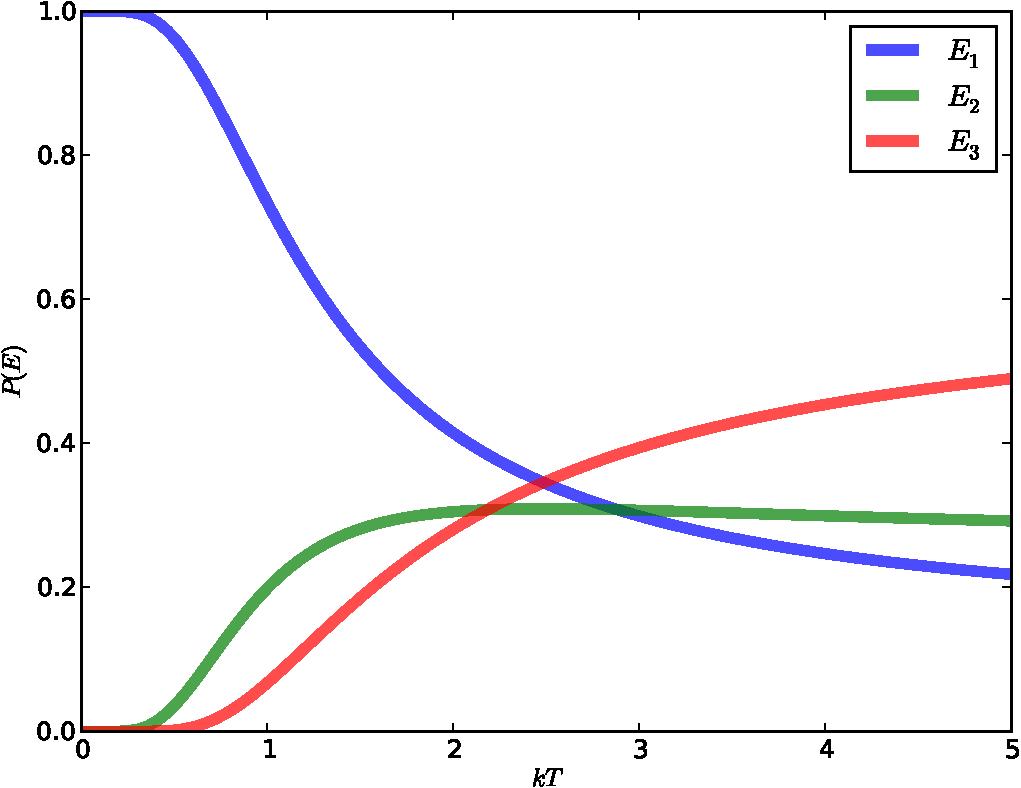
\includegraphics[width=.45\textwidth]{pictures/three_level_system/three_level_E-crop.pdf}}
  \subfloat[$C_V$]{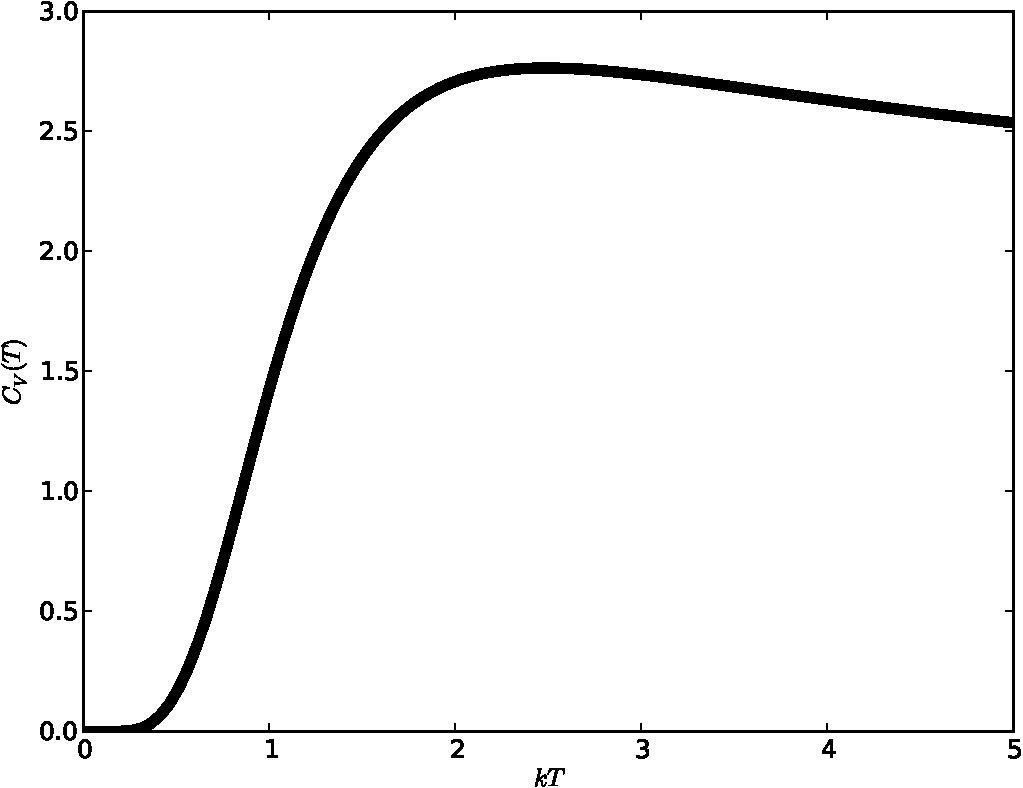
\includegraphics[width=.45\textwidth]{pictures/three_level_system/three_level_CV-crop.pdf}}
  \caption{Probabilities for each state of the sample three-level system (see Figure \ref{fig:sample_energy_level}) and the specific heat as a function of $1/\beta=kT$. }
  \label{fig:sample_energy_prob}
\end{figure}

%-------------------------------------------------------------------------------------

\section{Monte Carlo Methods}
\label{sec:monte_carlo}

In statistical mechanics we are not integrating a set of differential equations (as one would in the Classical or Quantum), but determining the distribution that satisfies the steady-state properties of a given Hamiltonian at a specific temperature. If the system is small and enumerable, such as the one we encountered in Section \ref{sec:ensemble}, we can evaluate the exact form of $\Z$. If the system displays self-similarity such as the Ising/Potts models 1D, 2D or over Cayley trees sometimes an analytical solution can be found.\cite{wu_potts_1982} In general however, the size state-space is too large and complex (and in the continuous case, too rough to discretize at a reasonable level) to completely solve for the states of the system. In general, one must use sampling methods to solve for the distribution. The etymology of the phrase `Monte Carlo' connects the random sampling of a physical system with the games of chance (whose profits also rely on random distributions) in the celebrated city of the same name in Monaco. 

\subsection{Metropolis-Hastings}
\label{sec:metroplis_hastings}

While many different adaptations of a Monte Carlo exist, the method most often used in physics simulations is the Metropolis-Hastings.\cite{metropolis_equation_1953} The Metropolis-Hastings algorithm is essentially a Markov transition matrix (a concept fully explained in Section \ref{sec:markov_matrix}). For each pair of valid conformations $(\xi_A, \xi_B)$ of the system (which need not be finite), there exists a corresponding matrix element that represents the transition probability. Not every state has to be connected to every other state, the only requirement is that connections between the conformations are ergodic, in that eventually every state will be reached from every other state. There exists a function called the move set which relates, from a given state, the accessible states to it.

The full Metropolis Hastings algorithm is a more general method of sampling then will be presented here, which will be confined to the simulation of physically relevant numerical experiments. From the canonical ensemble, the probability of observing a single conformation is $P(\xi_A) = \exp(-\beta E_A) / \mathcal{Z}$. When considering the ratio of two states, the partition function cancels leaving
\begin{equation}
  P(\xi_A \rightarrow \xi_B) = \frac{ \exp(-\beta E_A) } { \exp(-\beta E_B) } = \exp(-\beta \Delta E)
  \label{eq:metroplis_hastings_formula}
\end{equation}
with $\Delta E = E_A - E_B$. Hence, by using a move set function and starting from an initial conformation $\xi_0$ one proceeds to sample the state space by accepting or rejecting new conformations based on the probability in Equation \ref{eq:metroplis_hastings_formula}. 

This method, and others like it, generate a canonical distribution at a fixed temperature. The primary disadvantage is the lack of data over a significant range of temperatures, making multiple simulations necessary for the calculation of thermodynamic quantities. At low temperatures the algorithm can get stuck in local minima, severely impacting convergence rates. Various methods have been proposed to counteract this shortcoming, simulated annealing\cite{kirkpatrick_optimization_1983} being the most popular. In addition, near phase transitions the system can exhibit a critical slowing down, making the convergence extremely slow.\cite{yahata_critical_1969} 

\subsection{The Wang-Landau Density of States Method}
\label{sec:wang_landau}

Wang-Landau (WL) sampling\cite{wang_determining_2001} is a generic algorithm to calculate the relative density of states (DOS) for a given system. The algorithm starts off with the initial \textit{a priori} \textit{ansatz} that all conformational states are equally likely $\Omega(\xi)=1$, where $\xi$ is a conformation of the system.  Traditionally the calculation of the density of states was computed as a function of the energy of the system. Like others, we extend the use the Wang-Landau method to determine the the density of states for a set of conformations of the system rather than the energy explicitly.\cite{patel_effect_2008, wust_versatile_2009} This allows the system to be sampled for all values of the free variables simultaneously as the conformations can be turned into energies later.

In the WL method, the density of states is iteratively refined, crudely at first to ensure a large sampling, and then with greater precision as $\Omega$ converges. Similar to a typical Monte-Carlo simulation the algorithm has an acceptance rate. However, unlike traditional Metropolis-Hastings simulations, the process can not be modeled as a Markov chain since the transition matrix itself is iteratively refined. The WL acceptance rate is
\begin{equation}
  P(\xi_A \rightarrow \xi_B) = \min 
  \paren{ 
    1, \frac{\Omega(\xi_A)}{\Omega(\xi_B)} \frac{n_{B \rightarrow A}/n_B}{n_{A \rightarrow B}/n_A} 
  }
\end{equation}
Where $n_A$ is the number of outgoing moves from states $A$ and $n_{A \rightarrow B}$ is the number of moves from $A$ to $B$ (similarly defined for $n_B$ and $n_{B \rightarrow A}$). If the moves are reversible then $\frac{n_{B \rightarrow A}}{n_{A \rightarrow B}}=1$. These factors are necessary for detailed balance if the move set chosen has a variable number of moves from each state. Once any particular state had been selected the density of states is modified by $\Omega(\xi) \rightarrow f\Omega(\xi)$ where $f$ is a constant that is slowly reduced to unity during the simulation. 

It is important to note that the process is iterative, which has its advantages and disadvantages. Since the process uses the previous value of the density of states to determine the next refinement, excellent speedups can be obtained if one has any prior information about the distribution of the conformational degeneracies of the system. This may come from a previous simulation or general knowledge (for example, the 2D Ising model is roughly quadratic in log space). However, unlike the traditional Metropolis-Hastings models, the iterative refinement of the density states makes the process unable to be mapped to a Markov chain. This severely limits the analytic treatment that can be applied when discussing the convergence rates and saturation of errors. Several adaptions have been proposed to improve the algorithm. One can minimize the saturation of errors using an N-fold way process\cite{belardinelli_wang-landau_2007} with a steadily decreasing constant. One can also modify the move set in an optimal way to improve convergence.\cite{wu_overcoming_2005}

If the state space is not discrete, additional considerations have to be made. For the algorithm to generate a histogram, the continuous state space has to be discretized. Without prior knowledge of the system this can be difficult. If the level spacing is to small then the algorithm may fail to converge in a reasonable amount of time. If the level spacing is too large it may obscure the results, especially where the derivative of the density of states is large. To partially mediate the problem, we provide an approximation to the specific heat (a typically sought after parameter) in Appendix \ref{chap:macrostate_approx}.

%----------------------------------------------------------------------------------------

\section{Networks and Graphs}
\label{sec:graph_introduction}

This section introduces the idea of a graph. A graph $G$ is a collection of vertices $\{v_1, v_2, v_3, ...\} \in \mathcal{V}$ and edges $\{e_1, e_2, e_3, ...\} \in \mathcal{E}$. An edge is defined by the two vertices connecting to it, $e_i = (v_a, v_b)$. If the graph is directed then the ordering matters, \ie  the edge $(n_a, n_b)$ points only from $n_a$ to $n_b$. If the graph is undirected then the an edge is considered to point both ways. The edge set $\mathcal{E}$ for a graph contains only unique entries, as opposed to multi-graphs where this restriction is relaxed. Edges can carry a weight which we associate with each edge $\{e_1 : w_1, ..., e_i : w_2\}$. A vertex can also have a weight, and is associated the same way, $\{v_1 : n_1, ..., v_i : n_2\}$. If a graph has an edge connection to itself $e_i = (n_j, n_j)$ this edge is called a loop. Undirected, loop-free graphs are called simple graphs.

A useful device for keeping track of graphs is the adjacency matrix. In this matrix, the non-zero entries are those where an edge connects vertices $v_i$ to $v_j$
\begin{displaymath}
  \B{A}_{ij} = \piecewisebrace{
    \begin{array}{l r l}
      1 & : & e_k = (v_i, v_j) \in \mathcal{E}\\
      0 & : & \text{otherwise}
    \end{array}
  }
\end{displaymath} 
%
As an example, see Figure \ref{fig:example_graph_5node}, for a simple graph whose adjacency matrix is
\begin{equation}
  \B{A} = 
  \begin{bmatrix} 
    0 & 0 & 1 & 0 & 0 \\
    0 & 0 & 1 & 0 & 0 \\
    1 & 1 & 0 & 1 & 1 \\
    0 & 0 & 1 & 0 & 1 \\
    0 & 0 & 1 & 1 & 0 \\
  \end{bmatrix}
  \label{eq:example_graph_5node}
\end{equation}
\begin{figure}[ht]
  \begin{center}
    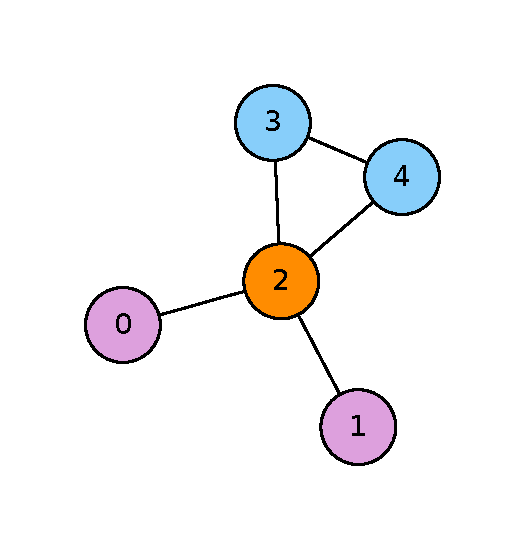
\includegraphics[width=\figurewidthTRIPLE]{pictures/graph_examples/example_simple_graph.pdf}
  \end{center}
  \caption{ 
    Pictorial representation of the graph given by the adjacency matrix, Equation \ref{eq:example_graph_5node}. The vertices are colored according to the walking polynomial defined in Equation \ref{eq:walking_polynomial}. }
  \label{fig:example_graph_5node}
\end{figure}
%
The adjacency representation is computationally useful, with it various graph properties can be calculated with ease. For example, one can show that $(\B{A}^2)_{ij}$ is the number of paths from $v_i$ to $v_j$ in exactly two steps. This holds in general, $(\B{A}^n)_{ij}$ is the number of paths from $v_i$ to $v_j$ in exactly $n$ steps. This connection between repeated iterations of multiplication makes simple graphs a natural study in the context of Markov matrices. 

\subsection{Graph Operations}
We will find it useful to perform two specific operations on the structure of the graph itself. The first, \emph{edge removal}, is simple. We define the operation $G_{-e_{ij}}$ to be the graph constructed from the edge set of $G$ with the edge $(v_i, v_j)$ removed. It is worthwhile to note that edge removal may split the graph into two disconnected subgraphs. If this happens we denote the subgraphs $G_1$ and $G_2$ as $G_{-e_{ij}} = G_1 \sqcup G_2$. The second operation, \emph{edge contraction}, is denoted by $G_{/ e_{ij}}$. In edge contraction vertices $v_i, v_j$ are merged into a new vertex $v_k$. All vertices that previously joined to $v_i$ or $v_j$ are now joined to the new vertex $v_k$. This operation can turn a simple graph into a non-simple one due to the presence of multiple edges. If this is the case, then the graph lacks a nice representation of an adjacency matrix (but it still can be referred to through its edge set $\mathcal{E}$). Representations of the two operations are shown in Figure \ref{fig:example_graph_5node_operations}.
\begin{figure}[ht]
  \begin{center}
    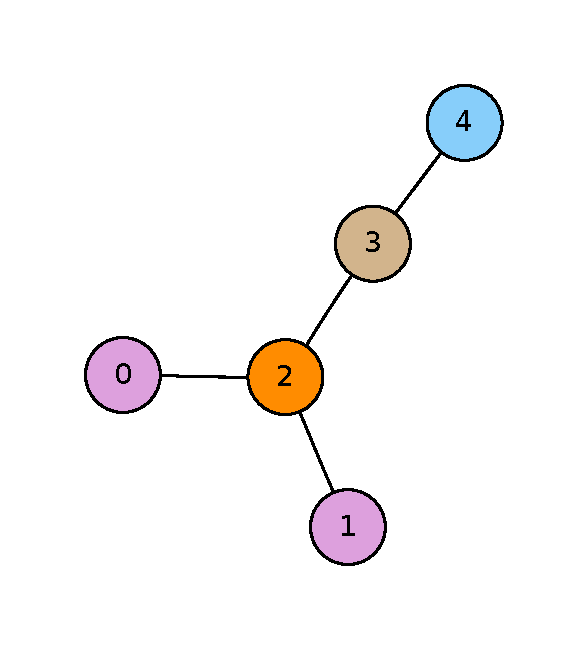
\includegraphics[width=\figurewidthTRIPLE]{pictures/graph_examples/example_simple_graph2.pdf}
    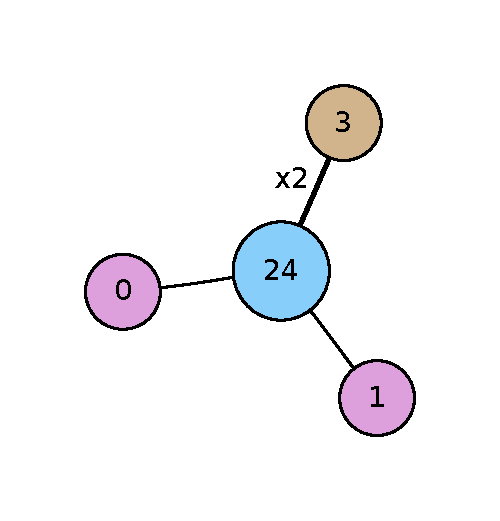
\includegraphics[width=\figurewidthTRIPLE]{pictures/graph_examples/example_simple_graph3.pdf}
  \end{center}
  \caption{Examples of edge removal (left) and edge contraction (right) of the edge $(v_2, v_4)$ on the graph shown in Figure \ref{fig:example_graph_5node}. Each operation removes exactly one edge. In this case edge contraction has made the graph non-simple due to the presence of a multi-edge (indicated by the x2.}
  \label{fig:example_graph_5node_operations}
\end{figure}

\subsection{Graph Isomorphism}
The ability to quickly determine if two graphs are isomorphic has attracted the attention of physicists, chemists, computer scientists and mathematicians for years. It is a long-standing open problem in both pure mathematics and its application. Graph structures are a common theme throughout this thesis, making the study of graph isomorphism relevant to many of the computations. For an approximate answer the problem is considered solved for most cases with the software \textit{nauty}.\cite{mckay_nauty} On a purely theoretical level, the exact solution is unique in terms of computational complexity. It is proposed that the problem is outside of the $\cal{P}$ vs $\cal{NP}$ class.\cite{schoning_graph_1988} Despite the growing number of invariants proposed, the graph isomorphism problem remains unsolved. Its ability to occupy the scientific world has been enough to label it as a plague on the community.\cite{read_graph_1977}

Nevertheless, we propose another invariant, the walking polynomials,  and do so with three goals in mind. The first is to expand upon the arsenal graph theorists have to determine basic properties of a particular graph. The second is the identification that the walking polynomials lend themselves naturally to a coloring scheme that allows the viewer to quickly identify the symmetries of the graph. Finally it is conjectured that the walking polynomials serve as a polynomial-time test to determine if two graphs are isomorphic.

The motivation for the algorithm comes naturally from the study of diffusive processes. The finite limit of a diffusive process is a collection of random walks along a graph. We can count (and solve) for a closed form expression for the number of closed loops along a graph starting at any particular vertex. A generating function can be constructed, one that encodes the path length of \textit{all} walks. It is with these generating functions we construct the invariant known as the walking polynomial.

\subsubsection{Walking Polynomials}
Given a graph with its associated adjacency matrix ${\bf A}$ define 
${\bf S} = ({\bf I} - {\bf A}z)$ and the walking polynomial matrix
\begin{equation}
  {\bf W}(z) = {\bf S}^{-1} = ({\bf I} - {\bf A}z)^{-1}
\end{equation}
%
Which can be computed without taking the inverse via Cramer's rule
\begin{equation}
  {\bf W}_{ij} = \frac{\text{minor}_{ij} {\bf S}} { \text{det} ({\bf S})}
  \label{eq:walking_polynomial}
\end{equation}
The set of diagonal elements $\{ {\bf W}_{11}, {\bf W}_{22}, \ldots, {\bf W}_{nn} \}$ represent the generating functions\footnote{
  It is often the generating functions themselves one is interested in, not any particular term. However, one can extract the $n$\textsuperscript{th} term from the infinite series by differentiating $n$ times to the desired term and setting all higher powers to zero.
  \begin{equation}
    f_{ij}[n](z) =
    \frac{1}{n!}
    \brackets{
      \pfrac{^ n }{ z^n } f_{ij}(z) 
    }
    _{z=0}
    =
    \frac{1}{n!} 
    \brackets{ 
      \pfrac{ ^n }{z^n} \frac{ p_{ij}(z) } { q(z) }
    }
    _{z=0}
  \end{equation}
  %
  If the generating function is a rational function and a closed form is sought, one can perform a partial fraction decomposition. Usually, known relations can reduce the solution to a closed form from this point. In addition, this exposes the poles for asymptotic analysis.
}
for the number of return paths to that vertex. Let an ordered set of these diagonal elements be called $\mathcal{W}$. The choice of ordering is irrelevant, only that it unambiguously sorts rational polynomials. We refer to $\mathcal{W}$ as the walking polynomial for short. We claim that $\mathcal{W}$ is a polynomial time computable invariant.

Take two graphs $G$, $G'$ with adjacency matrices ${\bf A}$, ${\bf A'}$, the matrices ${\bf S}={\bf I}-{\bf A}z$, ${\bf S}'={\bf I}-{\bf A'}z$ and their walking polynomial invariants $\mathcal{W}$, $\mathcal{W'}$. We say that two walking polynomials are equivalent $\mathcal{W} \sim \mathcal{W'}$ if and only if for every $w_i \in \mathcal{W}, v_i \in \mathcal{W}$ we have $w_i = v_i$. By definition, graphs $G$ and $G'$ are isomorphic if and only if there exists a permutation matrix ${\bf P}$ such that
\begin{equation}
  {\bf P A P} ^{-1} = \bf A'
\end{equation}
%
\B{Proof:} \begin{proof}[If $G$ and $G'$ are isomorphic then $\mathcal{W} \sim \mathcal{W'}$] Since $G$ and $G'$ are isomorphic let $\B{P}$ be the permutation matrix ${\bf P A P} ^{-1} = \bf A'$ and $\sigma({\bf P}) \in \{-1, 1\}$ be the the parity of the permutation. The denominator of each of the terms in $\mathcal{W}, \mathcal{W'}$ are related by
  \begin{equation}
    \det({\bf S}) = ({\bf P}) \det({\bf S'})
  \end{equation}
  %
  Given that the permutation matrix maps the numbers $(1, 2, \ldots, N) \rightarrow (k_1, k_2, \ldots, k_N)$ we have
  \begin{equation}
    \text{minor}_{i, i} ({\bf S}) = \sigma({\bf P}) \text{minor}_{k_i, k_i}( {\bf S'} )
  \end{equation}
  %
  Thus for each element $w \in \mathcal{W}$ there must be an element $w' \in \mathcal{W'}$ such that $w = w'$ and hence $\mathcal{W}$ is a graph invariant.
\end{proof}

%----------------------------------------------------------------------------------------


\section{Markov Matrix}
\label{sec:markov_matrix}

A Markov matrix $\B{M}$ is a matrix where each element $\B{M}_{ij}$ describes the probability of a transition from $i \rightarrow j$ in a single time step. As such each row represents a probability distribution
\begin{align}
  \sum_j \B{M}_{ij} & = 1 \\
  0 \leq \B{M}_{ij} & \leq 1
\end{align}

We say that a matrix is positive if all matrix elements are strictly greater then zero $(\forall i,j \hspace{1em} \mathbf{A}_{ij} > 0)$. A matrix is called primitive if there is a $k > 0$ such that $\mathbf{A}^k$ is a positive matrix. Physically, this implies that the matrix becomes well-mixed, and as we will see shortly, allows for the definition of a unique steady-state. If we view the Markov matrix as a graph whose edges are are weighted according to the matrix entries, we see that a disconnected graph implies a non-positive matrix. This typically, is not a problem as the matrix can be broken into separate subgraphs whose solutions are independent. There are however, insidious pathological matrices such as
\begin{equation}
  \B{P} = 
  \begin{bmatrix} 
    0 & 1 \\
    1 & 0 \\
  \end{bmatrix}
  \label{eq:example_non_positive_matrix}
\end{equation}
Here we see that $\B{P}^k=\B{P}$ for all odd $k$, implying that an initial condition in either state will elastically jump and never mix. Connected matrices such as $\B{P}$ are rare in practice however, since a tiny random perturbation to each of the matrix elements $\B{P}_{ij} \rightarrow \B{P}_{ij} + \epsilon_{ij}$ (that preserves the row sums value of unity and keeps all elements non-negative) will force the matrix to become primitive. 

Powers of the matrix describe longer jumps, \ie $(\B{M}^5)_{ij}$ describes the probability of ending up at state $j$ starting at state $i$ after five time steps. The process can be continued indefinitely, but for any primitive matrix, all initial conditions will converge to the same steady state vector. The largest eigenvalue of a primitive Markov matrix is unique and equal to unity, a consequence of the Perron-Frobenius theorem.\cite{perron_zur_1907} Due to the restriction on the row sums, all other eigenvalues are real. The associated eigenvector is then the unique steady-state vector. Intuitively, with only knowledge of the spectra of the eigenvalues, one can deduce this must be so. A large matrix power can be Schur decomposed into a matrix of eigenvectors $\B{V}$ and a diagonal matrix $\B{\Lambda}$ of the eigenvalues by $\B{M}^k = \B{V} \B{\Lambda}^k \B{V}^{-1}$. Since, for diagonal matrices we have $(\B{\Lambda}^k) _ {ij} = (\B{\Lambda}_ {ij})^k$ the appearance of a unique steady-state vector is consequence of the fact that the smaller eigenmodes will decay with time, leaving only the dominant eigenmode.

If the underlying graph of the matrix is disconnected, there will be a multiplicity $k$ in this unit eigenvalue, where $k$ is the number of disconnected pieces in the graph. Since the graph can be permuted into block diagonal form (with $k$ blocks), the degeneracy in the unit eigenvalue corresponds to the unique solution of each separate subgraph.

As an example, let's put weights on our graph (Figure \ref{fig:example_graph_5node}) from the previous section. We will use this matrix as an example to explain the concepts discussed below. To make matters simple, let's assume the probability of leaving (or staying) at any particular vertex is equiproportional, giving us the Markov matrix
\begin{equation}
  \B{M} = 
  \begin{bmatrix} 
    1/2 & 0 & 1/2 & 0 & 0 \\
    0 & 1/2 & 1/2 & 0 & 0 \\
    1/5 & 1/5 & 1/5 & 1/5 & 1/5 \\
    0 & 0 & 1/3 & 1/3 & 1/3 \\
    0 & 0 & 1/3 & 1/3 & 1/3 \\
  \end{bmatrix}
  \label{eq:example_markov_5node}
\end{equation}

As stated, all possible states of the system can be expressed by powers of this matrix. It is useful however to specify a specific state of the system, given as a distribution of over the vertices. For example, consider the initial condition such that all states are localized on vertex $v_1$ (given by the second row of the matrix). We would represent this condition by the vector
\begin{equation}
  \B{v}_0 = [0,1,0,0,0]^T
\end{equation}
One iteration of the Markov matrix with this initial condition would give
\begin{equation}
  \B{M} \B{v}_0 = \B{v}_1 = [0,1/2,1/2,0,0]^T
\end{equation}
And subsequent iterations of the matrix give
\begin{align}
  \B{M}^2 \B{v}_0    &= \B{v}_2  = [1/10,7/20,7/20,1/10,1/10]^T \\
  \B{M}^3 \B{v}_0    &= \B{v}_3  = [3/25,49/200,217/600,41/300,41/300]^T \\
  \B{M}^{50} \B{v}_0 &= \B{v}_5 \approx [.133, .133, .333, .200, .200]
\end{align}
There are a couple of things of interest going on here. The third power of the matrix has strictly positive entries, implying that the matrix is primitive and has a unique steady state distribution. The Schur decomposition is
\begin{align}
  \B{M}           &= \B{V} \B{\Gamma} \B{V}^{-1} \\
  \B{\Gamma}_{ii} &= \{ 1, 0.592, 1/2, 0, -0.225 \}
\end{align}
This appearance of an eigenvalue of unity is not surprising since we know that matrix is primitive. The magnitudes of the other entries set the time-scales for the decay of the other eigenmodes. Even in such a simple system the convergence to steady-state is not monotonic. As we've seen, all modes with $\lambda_i < 1$ are transient and do not effect the steady state distribution. However, the modes close to $1$ may persist for long times (relative to a characteristic time). The state vector $\B{\pi}$, where the net flow away and to each vertex is zero can be stated as the vector satisfying the condition such that
\begin{equation}
  \B{\pi} \B{M} = \B{\pi}
\end{equation} 
\ie the left-eigenvector associated with the unit eigenvalue.

%--------------------------------------------------------------------------------------


\section{Master Equation (ME)}
\label{sec:master_equations}

The master equation is a set of first-order differential equations that describe the time-evolution of a discrete system. It was first introduced by Wolfgang Pauli\cite{pauli_1928_probleme} and later used by Glauber to study the kinetics of the Ising model.\cite{glauber_time-dependent_1963} The master equation relates the change in the probabilities of the occupation of the states $\Xi = \{\xi_1, \xi_2,\ldots, \xi_k \}$ through a vector $\B{p}(t) = [ p_1(t; \xi_1), p_2(t; \xi_2), \ldots] $. From the ME, one can derive many relations used in stochastic dynamics such as the Fokker-Planck equation and Langevin equations. Let the conditional probability of changing from states $\xi_i \rightarrow \xi_j$ be $w_{ij}$. The master equation is
\begin{equation}
  \frac{d}{dt} \B{p}(t) = \sum_{j \neq i} 
  \paren{ w_{ij} \B{p}_j - w_{ji} \B{p}_i }
\end{equation}

The rate of change of the probabilities depends only on the current state of the system, \ie the master equation describes a memory-less or Markovian process. Total probability is conserved
\begin{equation}
  \frac{d}{dt}  \sum_{p_i(t) \in \B{p}(t)} p_i(t) = 0
\end{equation}
%
The master equation can be cast into matrix form
%
\begin{equation}
  \frac{d}{dt} \B{P}(t) = - \B{W} \B{P}(t)
\end{equation}
%
where $\B{W}$ is the stochastic matrix
%
\begin{equation}
  \B{W}_{ij} \equiv
  \piecewisebrace{
    \begin{array}{lr}
      w_{ij}                  & : i \neq j\\
      -\sum_{k \neq j} w_{kj} & : i = j
    \end{array}
  }
\end{equation}
%
By definition the columns sums of $\sum_{i} \B{W}_{ij} = 0$ for all $j$, which is simply a restatement of the conservation of probability. Since the equations are only coupled first-order differentials, their solution is simply
\begin{align}
  \B{P} &= e^{\lambda t} \B{v}  \\
  \B{W} \B{v} &= \lambda \B{v}
\end{align}
%
In general, $\B{W}$ is not symmetric and therefore may have complex eigenvalues. However, any matrix with only real elements is guaranteed to satisfy
\begin{equation}
  \B{W} \B{v} = \lambda \B{v} \rightarrow \B{W} \B{v}^* = \lambda^* \B{v}^*
\end{equation}
Since the elements of $\B{W}$ are always real, the eigenvalues and their associated eigenvectors may be real, or complex conjugate pairs.

For an ergodic system with rate matrix $\B{W}$, the Perron-Frobenius theorem tells us that there is a unique eigenvalue $\lambda_1=0$ and all of the other eigenvalues must have a strictly negative real part. Furthermore the associated eigenvector $\B{v}_1$ must have only non-negative components. This eigenvector has a connection to the steady state probability and ensures that the probabilities are non-negative. All initial conditions of an ergodic system (excluding pathological cases) will approach a steady state vector $\B{\pi}$. A stronger condition is that of detailed balance which holds, if for each pair $i,j$
\begin{equation}
  \B{W}_{ij} \B{\pi} _{j} = \B{W}_{jk} \B{\pi} _{k}
\end{equation}
%
implying that around any closed cycle of states there is no net flow of probability. The master equation has a formal solution
\begin{equation}
  p_i(t) = \sum_{j} \sum_{k} \B{V}_{ik} \exp { \paren{\lambda_k t} } \B{V}^{-1}_{kj} p_j(0)
\end{equation}
%
For a stationary process, \ie a Markovian one, the transition probability depends only on the time interval between two events. Therefore we can write the solution as
\begin{align}
  p_i(t)
  &= [\B{V} \exp { \paren{ {\Gamma t} } } \B{V}^{-1}] p(0) 
  \\ 
  &= \B{M}(t) p(0)
\end{align}
%
Where $\B{M}(t)$ is the matrix exponential of the rate transition matrix. The exponential of a matrix always exists and can be found with a Taylor expansion.
%
\begin{equation}
e ^ {\B{A}} = \B{I} + \B{A} + \frac{1}{2!}\B{A}^2 + \frac{1}{3!}\B{A}^3 + \dots = \sum_{k=0}^{\infty}\frac{1}{k!}\B{A}^k
\end{equation}
If the matrix is diagonalizable it can be found by
\begin{equation}
e^{\B{A}} = \B{V} e^{\B{\Gamma}} \B{V}^{-1}
\end{equation}
Which is trivial since the exponential of a diagonal matrix is
\begin{equation}
\paren{ e^{\B{\Gamma}} } _{ij} = e^{\B{\Gamma}_{ij}} \delta_{ij}
\end{equation}
%
This gives the important relation between a Markov matrix and a rate matrix acting as its generator
\begin{equation}
  \B{M} = \exp(t \B{W}) .
\end{equation}

%---------------------------------------------------------------------------------------

  
  %CHAPTER: Entropic forces and Cosolute Flows
  \chapter{Entropic forces and Cosolute Flows}
\label{chap:entropic_force}

\section{Experimental Motivation}
When considering the structural dynamics and functionality of macromolecules, the effective volume of the surrounding environment is a  critical factor. Conditions in typical cellular environments are often filled with other molecules whose size is on the same order as macromolecules. As the environment gets crowded, the mutual impenetrability of the particles gives rise to excluded volume effects and has significant consequences for protein stability and folding rate,\cite{minton_can_2006, ping_depletion_2006, rosgen_protein_2005, pincus_crowding_2009, cheung_effects_2007, cheung_molecular_2005, stagg_molecular_2007, minton_models_2005, sasahara_effect_2003} chaperonin action\cite{zhou_protein_2004} and amyloid fibril formation.\cite{kinoshita_ordered_2004} Crowded environments may also enhance the rate of protein aggregation \cite{ellis_protein_2006}. A comprehensive review of macromolecular crowding can be found in \cite{huan-xiang_zhou_macromolecular_2008}. 

Along this line, two recent experiments are the motivation for the present work. The first is the single-molecule measurement of the mechanical force required to unfold a protein molecule (ubiquitin) using atomic force microscopy (AFM). It was found that at fixed pulling speed the unfolding force increased progressively as more crowders are added.\cite{yuan_effects_2008} Our model here assumes the globular protein is mainly spherical in shape and when stretched under the AFM, elliptic. Furthermore, while the protein molecules are under stretch they are not free to move. Therefore, for simplicity we consider the limiting case that the stretched protein is an infinitely heavy hard ellipse which is stationary under collisions with the crowder molecules. In this paper, we have restricted ourselves to a 2D system. 

%********************
The effect caused by the addition of cosolutes observed in these experiments is the result of the interplay of the entropic effect of the macromolecule, cosolute and water. Since the cosolutes added are typically hydrophilic, their addition causes an increase in the total packing fraction of the aqueous solution, leading to a stronger crowding effect.\cite{akiyama_remarkable_2006} Nevertheless, a single-component system is still a useful tool to elucidate the physical nature of the entropic excluded volume effect. Our work considers the dynamics of a large heavy solute immersed in a bath of hard-spheres to model these observations of crowding-enhanced protein stability.

%********************

Another related experiment showed that a crowded environment can induce shape change in protein molecules (Borrelia burgdorferi VIsE) from a non-spherical native structure to a more compact non-native spherical structure.\cite{homouz_crowded_2008} Associated with this shape change, the function of protein may change as a result. An interesting question to ask is then: Can a non-spherical molecule experience an intra-molecular attraction, somewhat similar to the role of  surface tension, change its shape into a spherical one due to the presence of crowders?  An objective of the present article is to try to answer this question by studying the collision dynamics between hard-disc crowders and a hard ellipse. 

The first study of excluded-volume effects, also known as the depletion force, was originally derived by Asakura and Oosawa\cite{asakura_interaction_1958} for hard spheres. AO theory assumes that the density of the crowders is uniform for all permissible volumes and the excluded volume is simply the volume of the offset shape. The offset for a single convex particle is defined as the surface extended some distance normally from the surface. The excluded volume modifies the partition function by restricting the space available to the particles. The closer two particles are, the more volume is available to the remaining crowders and hence a stronger depletion force. By simple geometric arguments, AO theory gives an attractive interaction for hard discs that scales monotonically with the inter-particle separation. Essentially this is the zeroth-order term in integral equation theories based on statistical mechanics. The true spatial distribution is dependent on pair-wise correlations, which themselves are dependent on three-point correlations, etc. To move beyond AO theory requires detailed knowledge of these higher-order correlation functions. The Ornstein-Zernike equation, an open equation that gives the exact distribution function, can be solved analytically under proper closure relations such as the Percus-Yevick (PY) relation for hard spheres,\cite{wertheim_exact_1963} and hard ellipses.\cite{ward_structure_1988} The PY closure gives good results for low size asymmetry and packing fractions, outside this domain it can lead to pathological results for the density profiles. An alternative closure relation, hypernetted-chain (HNC) \cite{van_leeuwen_new_1959} has been shown to give results more consistent with numerical simulations.\cite{kinoshita_interaction_1996}

This tendency of hard-disc or hard-sphere objects to feel an inter-particle entropic force has previously been observed in physical experiments,\cite{crocker_entropic_1999, ohshima_direct_1997} theoretical predictions,\cite{tehver_depletion_1999, mao_depletion_1995} and computer simulations.\cite{biben_depletion_1996} The impenetrability of the molecules, a nonspecific steric repulsion, forms the basis of this entropic force. The loss of entropy between the two particles is overcome by the gain in the entropy of the remaining particles. 

An interesting effect resulting from the theory of depletion force is the tendency for particles to move along surfaces of decreasing curvature for convex surfaces (and equivalently, increasing curvature for concave surfaces). The depletion zone a crowder makes at contact is greater for a flatter surface, hence the particle should, on average, feel a force in this direction. Studies of various geometries using integral theories\cite{kinoshita_interaction_2004, kinoshita_spatial_2002} and density functional theory\cite{roth_depletion_1999, roth_depletion_2000} have confirmed this fact. This has been experimentally observed for colloidal particles that feel repulsion near a sharp edge.\cite{dinsmore_entropic_1996} Manipulation of colloidal structures has an obvious appeal, but typically these studies focus on the density profiles and not the resulting velocity patterns that arise from the entropic interaction. In this chapter we provide evidence of the entropic flows arising from hard potential surfaces.

If a crowder tends to move along regions of decreasing depletion areas, one should observe a flow of entropic origin surrounding non-uniformly curved surfaces. If we vary the geometry of a fixed macromolecule, say from a circle to an ellipse, it is possible to change these density profiles and resulting flows.  We investigate this effect by varying the shape of the ellipse as well as the different packing fractions and the relative size of the crowders. 

In a biological system, water cannot be regarded as an inert background.\cite{kinoshita_roles_2006} The presence of a solute generates an excluded volume not only for the other solutes but also for water molecules. To exclusively investigate the entropic excluded-volume effect, water molecules can also be modeled as hard spheres. In a strict sense, ``crowders'' should be treated as a multi-component system.\cite{akiyama_remarkable_2006} However, considering water molecules explicitly in a multi-component system would greatly increase the complexity of the computation. We shall therefore focus on the depletion effects of one-component crowders on a non-spherical body in the present study.

%For a biological system, the solvent water molecules have unique properties, related to its dipole moment, the dielectric constant and its tendency to form hydrogen-bonded clusters. In the present study of the excluded volume effects between hard bodies, we do not take solvent into explicit consideration. If we do, the net excluded volume effect can be significantly greater, as shown by Akiyama \cite{akiyama_remarkable_2006} \emph{et al.} However, considering solvent molecules explicitly in a multicomponent system would greatly increase the complexity of the computation. We shall therefore focus exclusively on the depletion effects of crowders on a non-spherical body in the present study.

%The resulting microscopic structure of the solution certainly plays a role in determining the system properties. In a strict sense, one should consider both the crowders and the solvent explicitly as a multi-component system. Unlike true colloidal suspensions however, there are no biological systems that can be treated as hard-body models in real experiments \cite{kinoshita_roles_2006}. We therefore investigate the entropic effect exclusively in the present model by employing a hard-body potential of a large macromolecule immersed in a single-component solution.

This chapter covers the computational method first, detailing the design parameters and the implementation of the discrete molecular dynamics. This is followed by the results of the simulations, along with a quantitative analysis on the boundary condition itself. The final section outlines the importance of the velocity fields along with their connections to the original motivating experiments.

\section{Computer simulations}


\subsection{Simulation design}

In the present work, we examine the flow of hard-discs around a hard ellipse fixed at the origin. The entire simulation is done using discrete molecular dynamics (DMD) as each potential collision can be predicted analytically. Initially the time of first collision for all disc pairs is found, along with the interaction against the interior boundary condition. This list is chronologically ordered and the simulation is integrated to the first collision. The collision is handled, conserving energy and impact angle and the collisions for the interacting discs are recalculated with the new velocity vectors. 

Calculating a collision between hard-discs is trivial. Given two velocity vectors, initial positions and radii of $r_a, r_b$, the discs first intersect when the positions are exactly a distance of $r_a + r_b$ apart. The exact time of collision can be reduced to a quadratic equation, whose discriminant is zero when the discs do not collide.

The collision of a disc with any other closed surface is, in general, a difficult problem to solve analytically. If the shape is convex, then the disc can intersect with the surface at most four times. The first point of collision can be found by setting the discriminant to zero, corresponding to a multiplicity of the roots, or identically the first point of collision. The collision can then be found by plugging this solution into the general solution of the fourth order intersection polynomial. This collision can also be visualized as the first point of intersection between a line and the offset of the convex shape. If the offset has a simple form, the problem simplifies greatly. For a disc, the offset \textit{is} another disc, whose collision is trivial. For an ellipse the offset shape is complicated, often requiring an iterative solution. The problem of two translating, rotating ellipses can be solved however, by reducing the problem to the roots of a simpler eighth-order polynomial.\cite{yi-king_choi_continuous_2006}

\subsection{Boundary conditions}
Using a dimensionless unit of length $L$ the system of interest is enclosed in a two-dimensional square box centered at the origin. The side length was $2L$ using periodic boundary conditions. Each hard-disc was given an initial velocity vector in a random direction whose magnitude was drawn from Gaussian distribution. The interior boundary condition was an ellipse, whose offset was defined as the surface extended normally a distance $r$. The ellipse defined with axes $E_a,E_b$ was parametrized as
%
\begin{equation}
\vec Q(\phi) = \begin{bmatrix}
	E_a \cos \phi \\
	E_b \sin \phi \\ 
\end{bmatrix} \\
\end{equation}

The first point of contact made by a hard-disc of radius $r$ with the ellipse is the intersection of its velocity ray with the ellipse offset
%
\begin{equation}
\vec Q_{\textit{offset}} = \vec Q + r\hat N
\end{equation}
%
Where $\hat N$ is the outward unit vector normal to the surface. The parametric form for the offset shape is thus
%
\begin{equation}
\vec Q(\phi) = \begin{bmatrix}
	E_a \cos \phi  + g r E_b \cos \phi\\
	E_b \sin \phi  + g r E_a \sin \phi\\
\end{bmatrix} \end{equation}
%
where $g={((E_b \cos \phi)^2 + (E_a \sin \phi)^2)}^{-1/2}$.

\section{Results}

The crowders consisted of a fixed number $N=50$ of homogeneous hard-discs whose radius varied according to packing fraction values of $\Pi=0.10$ to $\Pi=0.30$ with fixed aspect ratio of $k \equiv E_a/E_b$. For comparison, cellular interiors show approximately 20-30\% volume occupation by macromolecules.\cite{ellis_macromolecular_2001} 

Statistical averages of the velocity and density fields were taken by dividing the system into $150^2$ square cells. Snapshots of the fields were taken after $1/5$ of the total simulation time to allow for an initial thermalizing of the system. The resulting density patterns shown in FIG. \ref{fig:density_plot} are complex, but similar to other studies of hard-solutes near boundary conditions. As an example, consider in FIG. \ref{fig:radial_plot} the density distributions plotted along the major and minor axes. Each curve is zero inside the depletion zone, then it exhibits characteristic oscillations on the length scale of the crowder diameter. The reason for this is well known, the crowder statistically prefers to form shells around immobile barriers. It is also clear from the earlier discussion that the density on-contact should be larger for the minor (flatter) axis of the ellipse, as the depletion force there is greater.

\begin{figure}
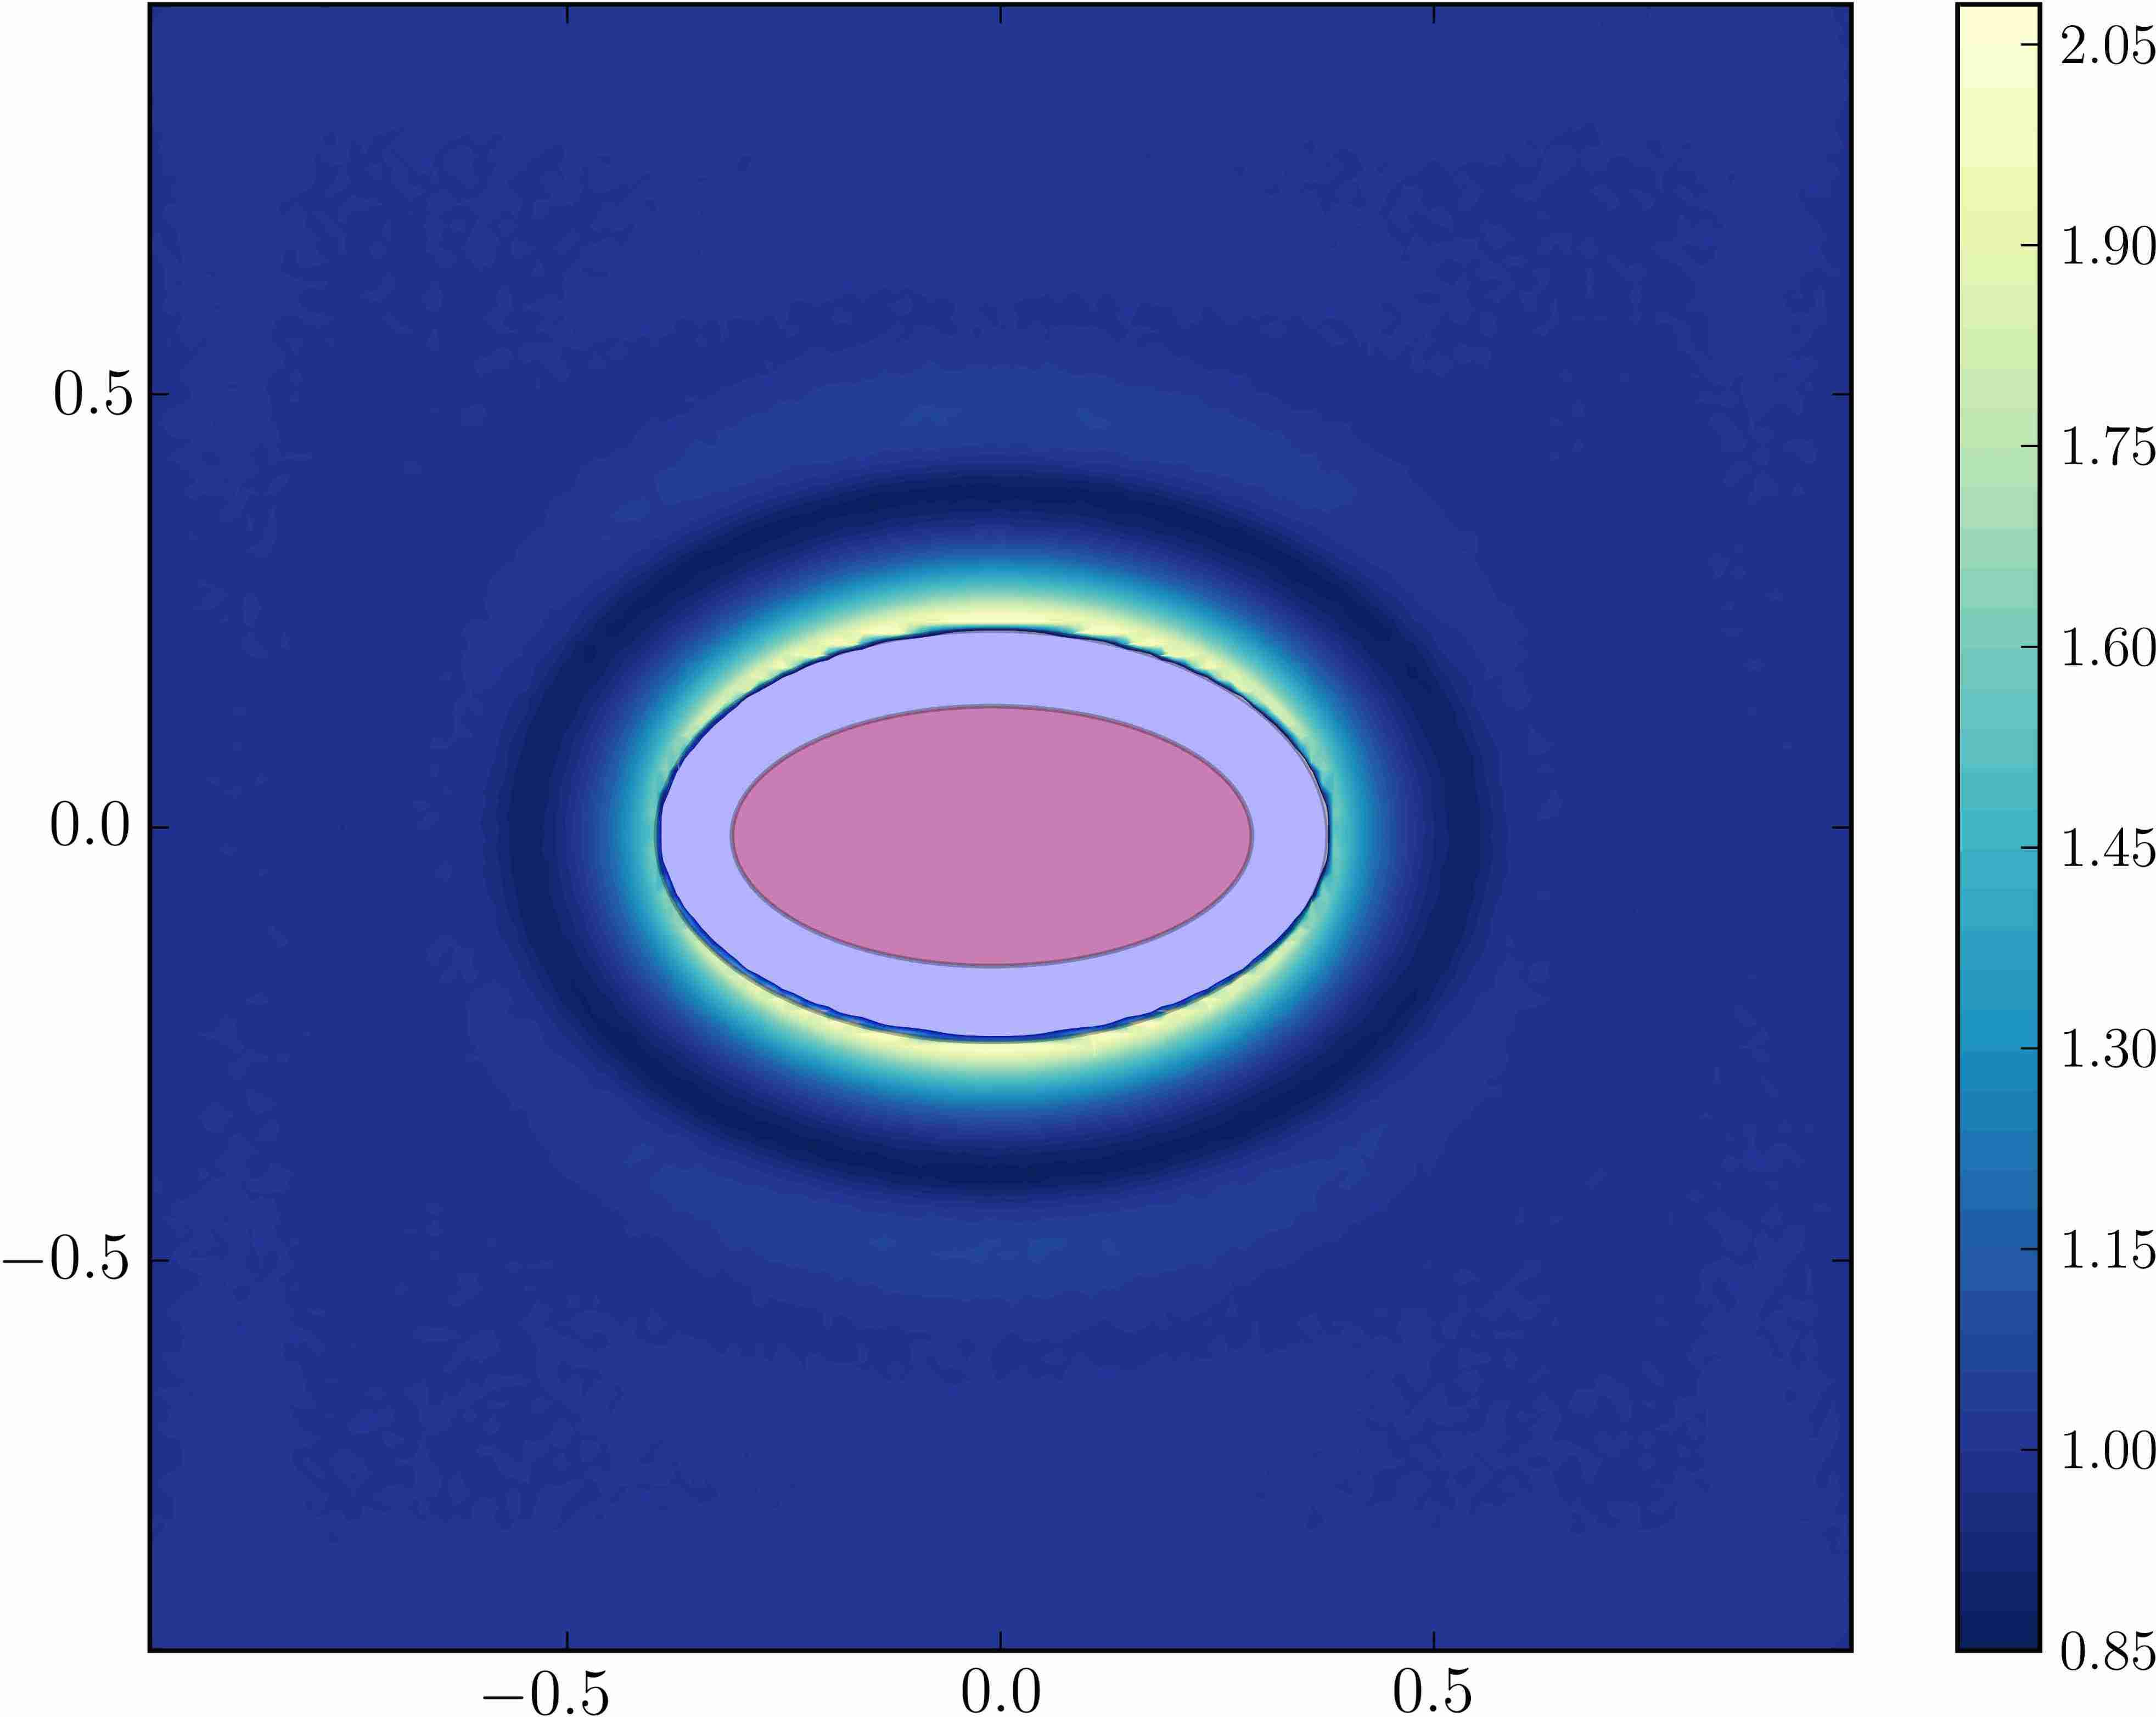
\includegraphics[width=\figurewidthSINGLE]{entropic_flow_paper/FIG1_EDIT.jpg}
\caption{Contours of averaged density profiles for an aspect ratio $k=2.0$, packing fraction $\Pi=0.30$, and relative crowder radius $r_c/L=0.04370$. The density has been normalized such that the bulk density is unity. Both the hard-ellipse and an approximation of the depletion zone are shown schematically.}
\label{fig:density_plot}
\end{figure}

\begin{figure}
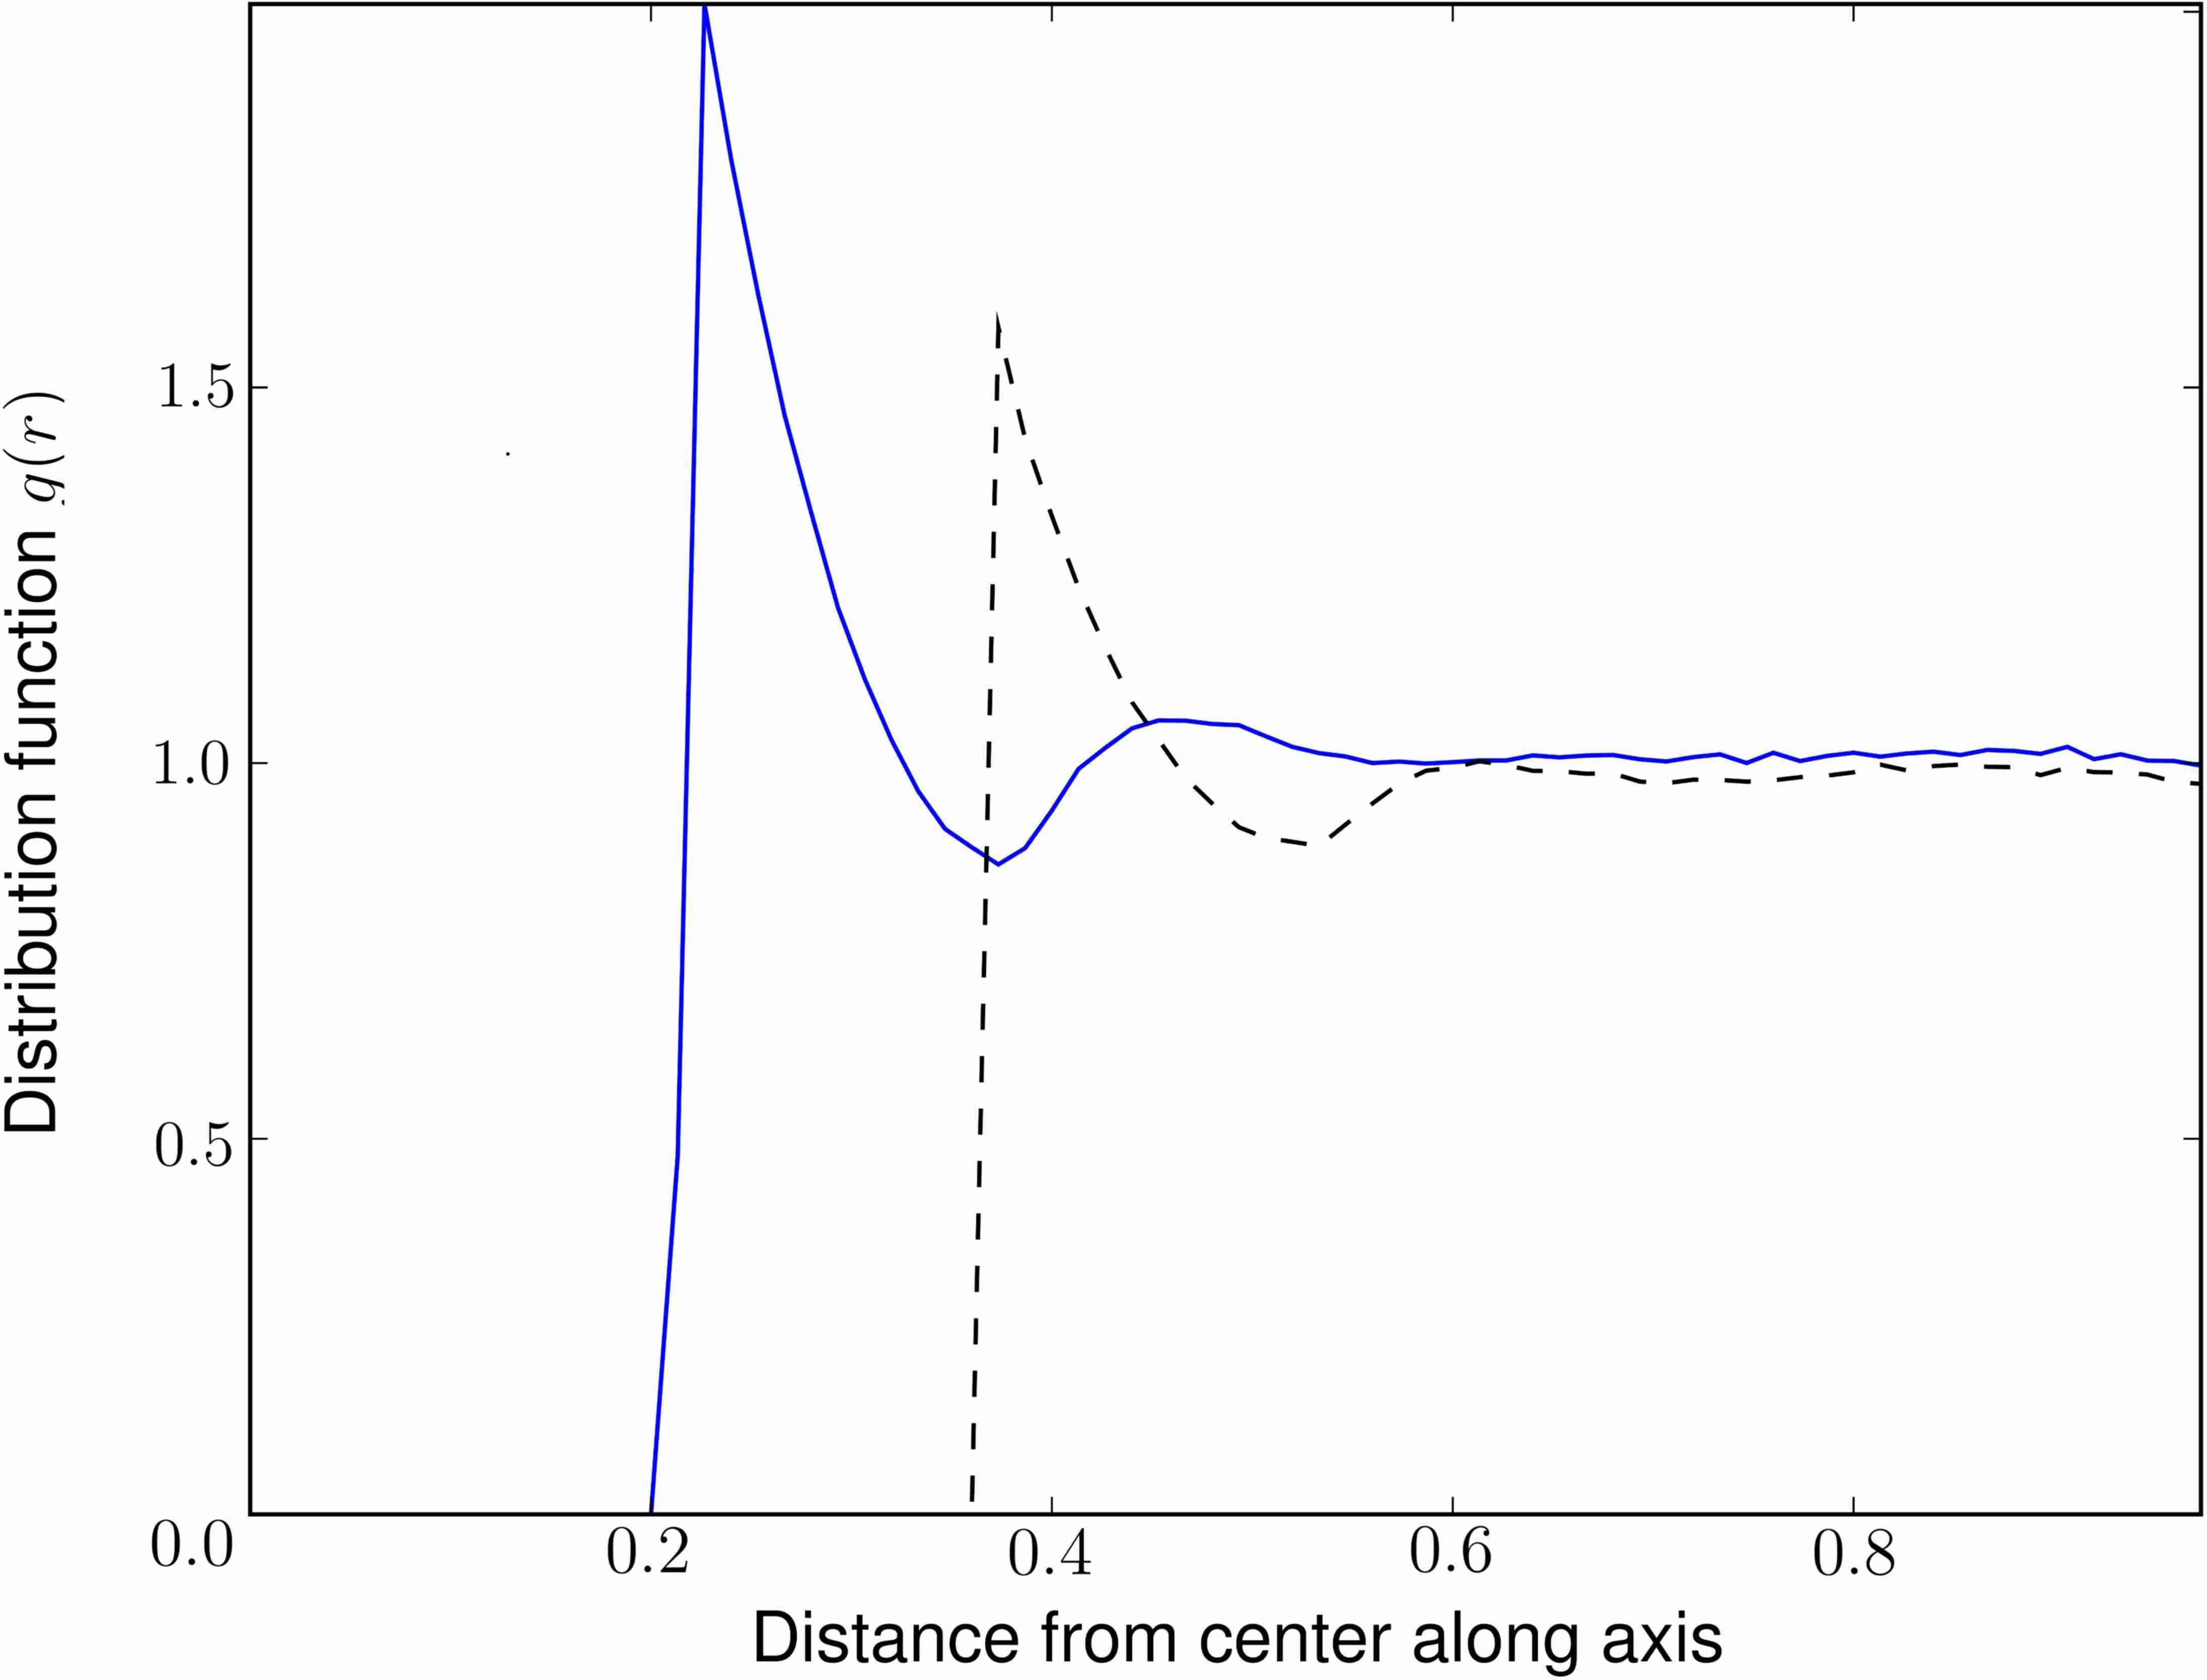
\includegraphics[width=\figurewidthSINGLE]{entropic_flow_paper/FIG2_EDIT.jpg}
\caption{Generalized distribution function along each elliptical axis for the parameters aspect ratio $k=2.0$, packing fraction $\Pi=0.30$, and relative crowder radius $r_c/L=0.04370$. The distribution function $g(r)$, is a measure of the average density at a point, normalized to one at the bulk density. The position of the function is to be taken from the origin along the specified axis, with the distance in units of $L$. The blue (solid) and black (dashed) curves denote the values along the minor and major axis respectively. The density on-contact is significantly greater at the minor axis of the ellipse. The curves exhibits characteristic oscillations at precisely the crowder diameter. }
\label{fig:radial_plot}
\end{figure}

Interestingly, when we plot the time-averaged velocity field near the hard ellipse the field exhibits four vortices. Since the system has four-fold symmetry (up to a sign change in the curl of the velocity field), we show only a portion of the upper quadrant of the velocity in FIG. \ref{fig:velocity_plot}. The velocity field clearly exhibits a single vortex, one that remains stable in both size and location for the duration of the simulation. The net angular momentum of the system is still zero as each vortex has a counter-rotating partner, but the distribution of the momentum has been partitioned along the quadrant lines. This is an initially surprising result, as such flows are usually caused by a thermal gradient, advective field or other potential. The entropic flows observed here are completely the result of treating the ellipse as a hard boundary (rather than a free particle), which serves to redistribute the angular momentum of the system. This is discussed further in next section. The exterior periodic boundary conditions serve to enclose the flow. It is unknown if the flows obtained are still valid in an infinite bath ($L \rightarrow \infty$). The deviation from uniformity of both the density and velocity fields occurs whenever $k \neq 1$. As the the aspect ratio approaches unity ($k \rightarrow 1$) the pattern generation takes longer to develop implying that there are no observed phase transitions.

\begin{figure}
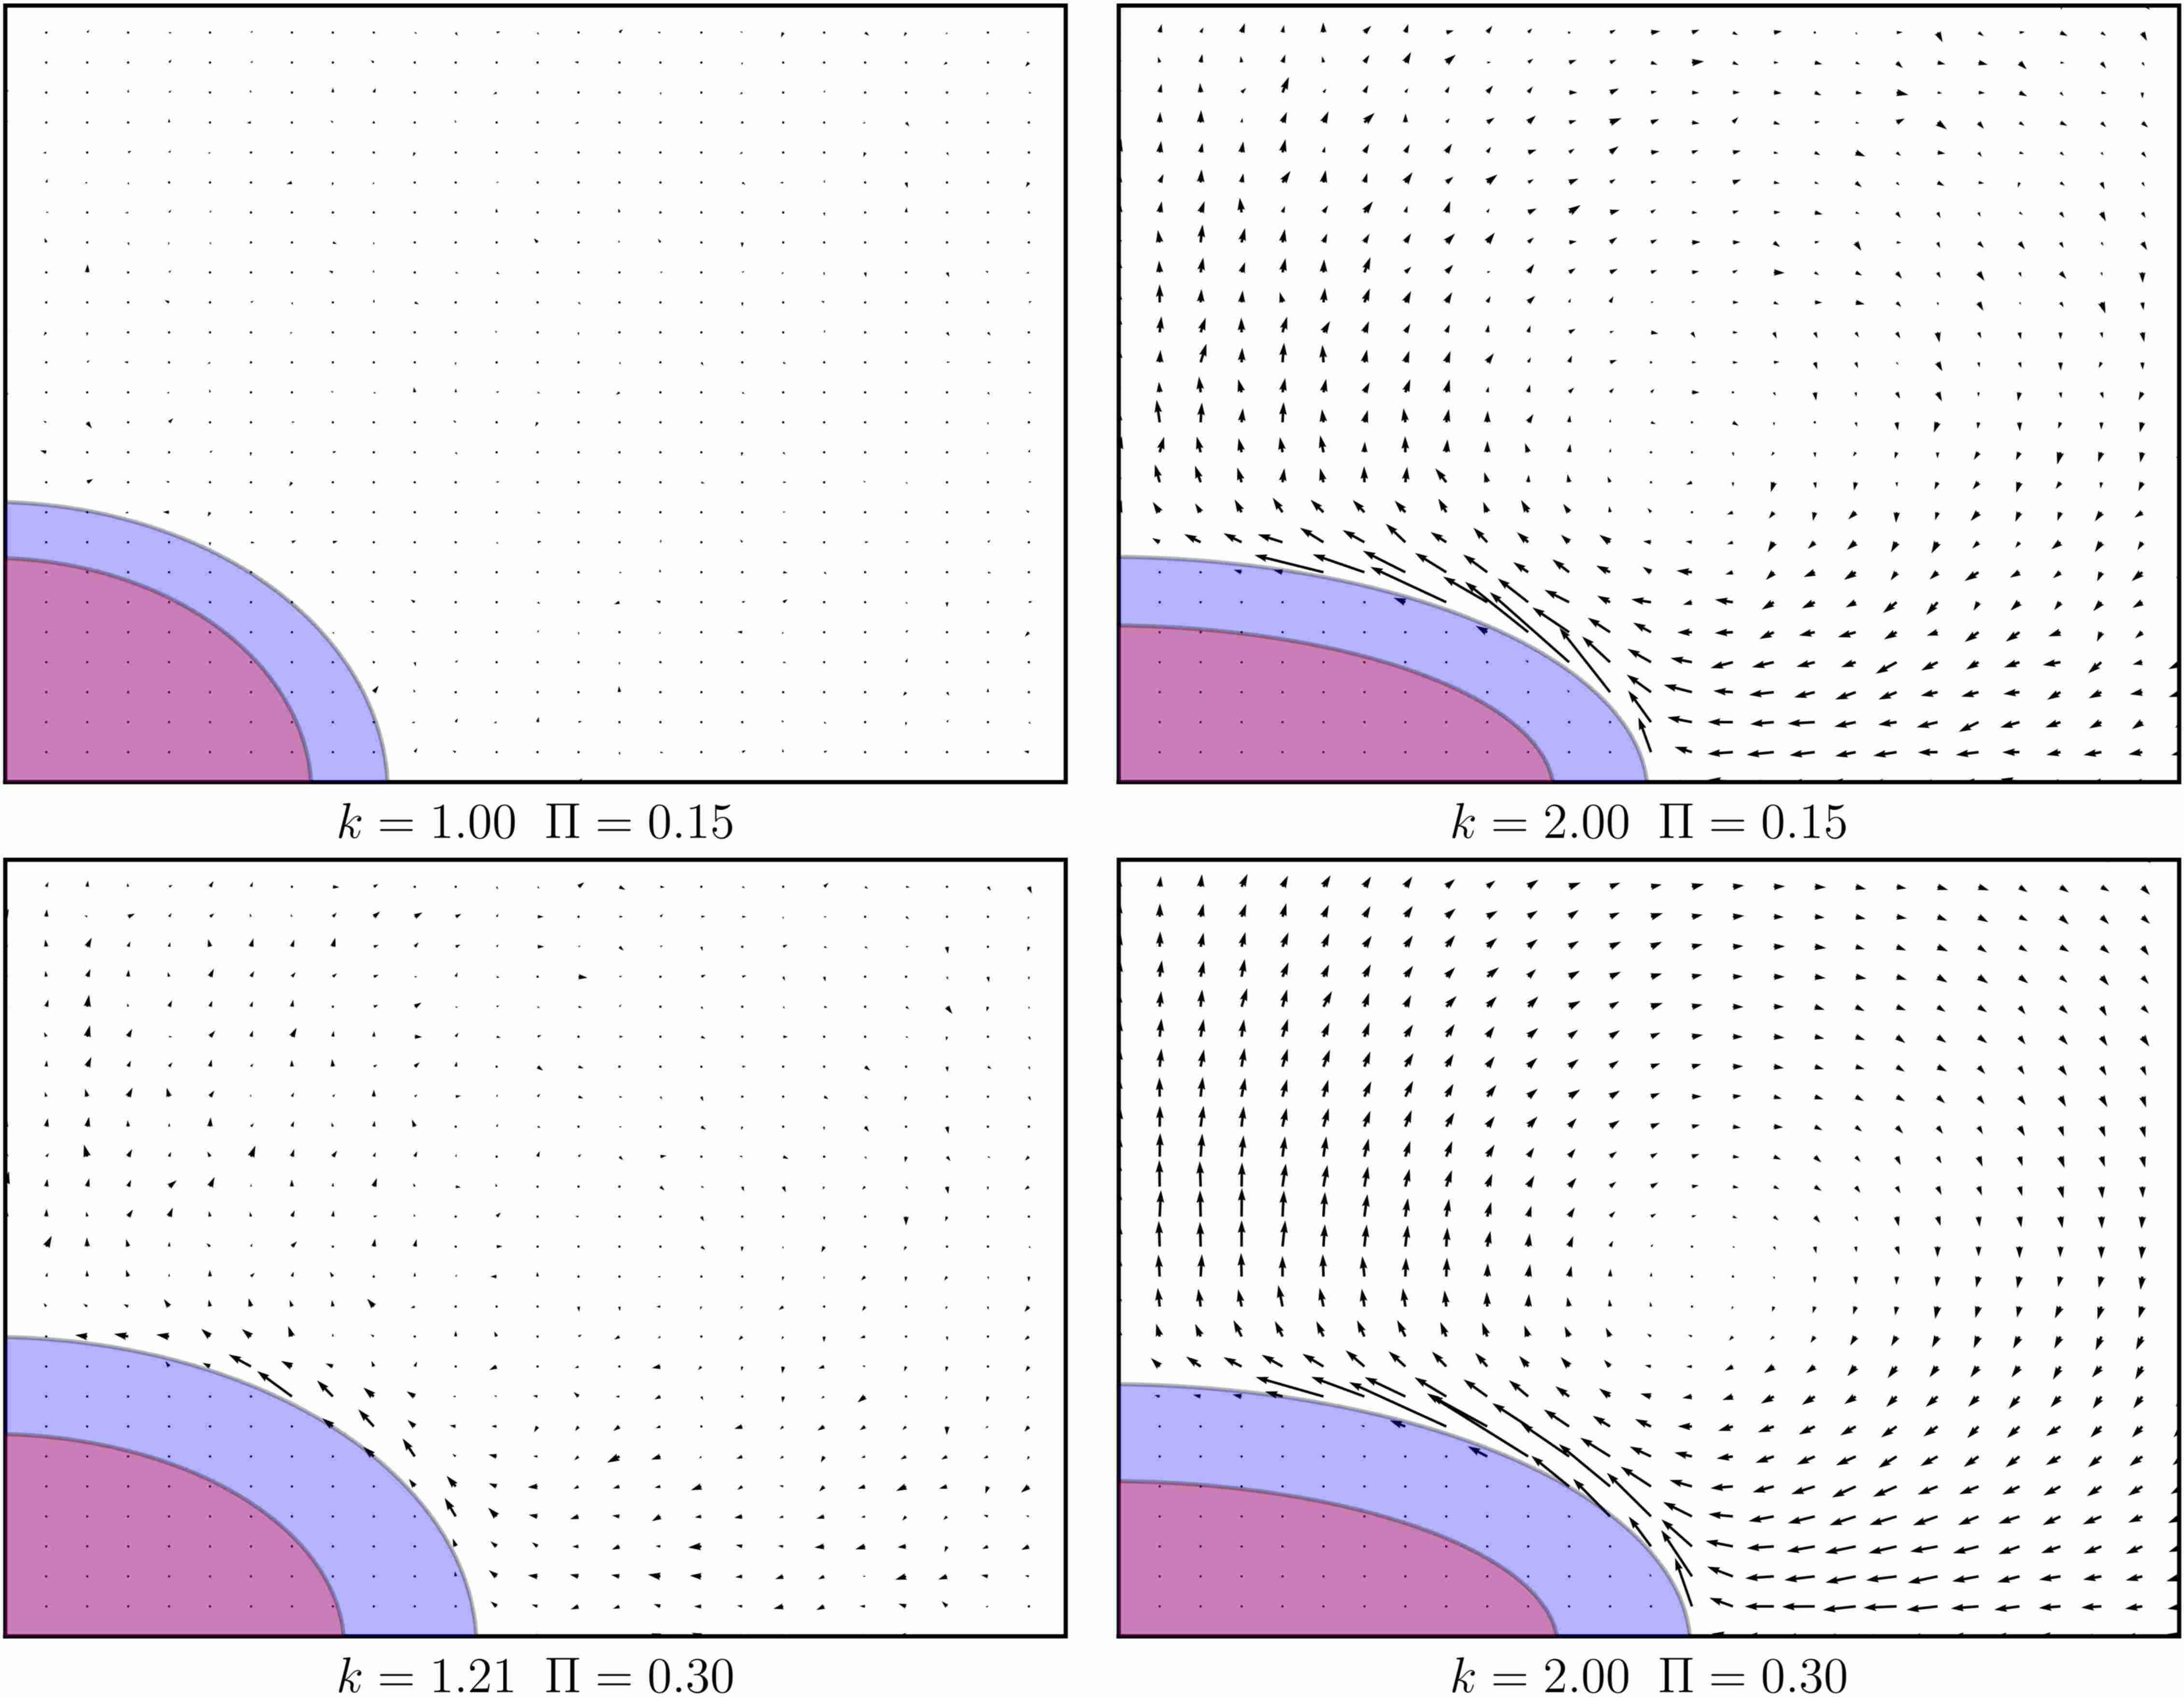
\includegraphics[width=15cm]{entropic_flow_paper/FIG3_fourvelocity.jpg}
\caption{Time-averaged velocity vectors in the upper right quadrant of the simulation for different parameters (shown on chart). For comparison of vector magnitudes the largest arrow in the lower-right graph corresponds to a velocity that is 6.4\% and 11.8\% of the average and median respectively of the initial velocity distribution. The general magnitude of the vectors is highly dependent on the aspect ratio, and disappears completely for a circle ($k=1$). Both the hard-ellipse and an approximation of the depletion zone are shown schematically. }
\label{fig:velocity_plot}
\end{figure}

Motivated by the time-averaged velocity contours which seem to imply a compressing force on the ellipse along the x-axis and an expanding force along the y-axis, an averaged pressure was calculated by recording all momentum changes of the crowder against the ellipse. The average pressure ratio, a heuristic measure designed to measure the tendency of the ellipse to deform, is
%
\begin{equation}
R \equiv \sum_{r,\Delta p \in C}{ \frac{1}{k} \frac{{ \Delta p_x \sgn(r_x) }}{{\Delta p_y \sgn(r_y) } } }
\end{equation}
%
where the sum extends over the set $C$ of all recorded collisions of the crowders against the ellipse, $r,\Delta p$ represent the  position and the change of momentum vectors over the duration of the collision, respectively, with the subscripts indicating the component along the indicated direction, and $\sgn$ is the sign function.

$R$ is a positive function over both increasing aspect ratio and crowder density as show in FIG. \ref{fig:Pratio_plot}. Furthermore it shows the scaling of $R$ is roughly quadratic over an increase of the aspect ratio. Values of $R>1$, more pressure against the major axis, suggest a return to a spherical shape. The results obtained show that the presence of crowders near a fixed aspherical molecule is not the favored state, one that becomes increasingly unfavorable in both crowded conditions and aspect ratio. 

\begin{figure}
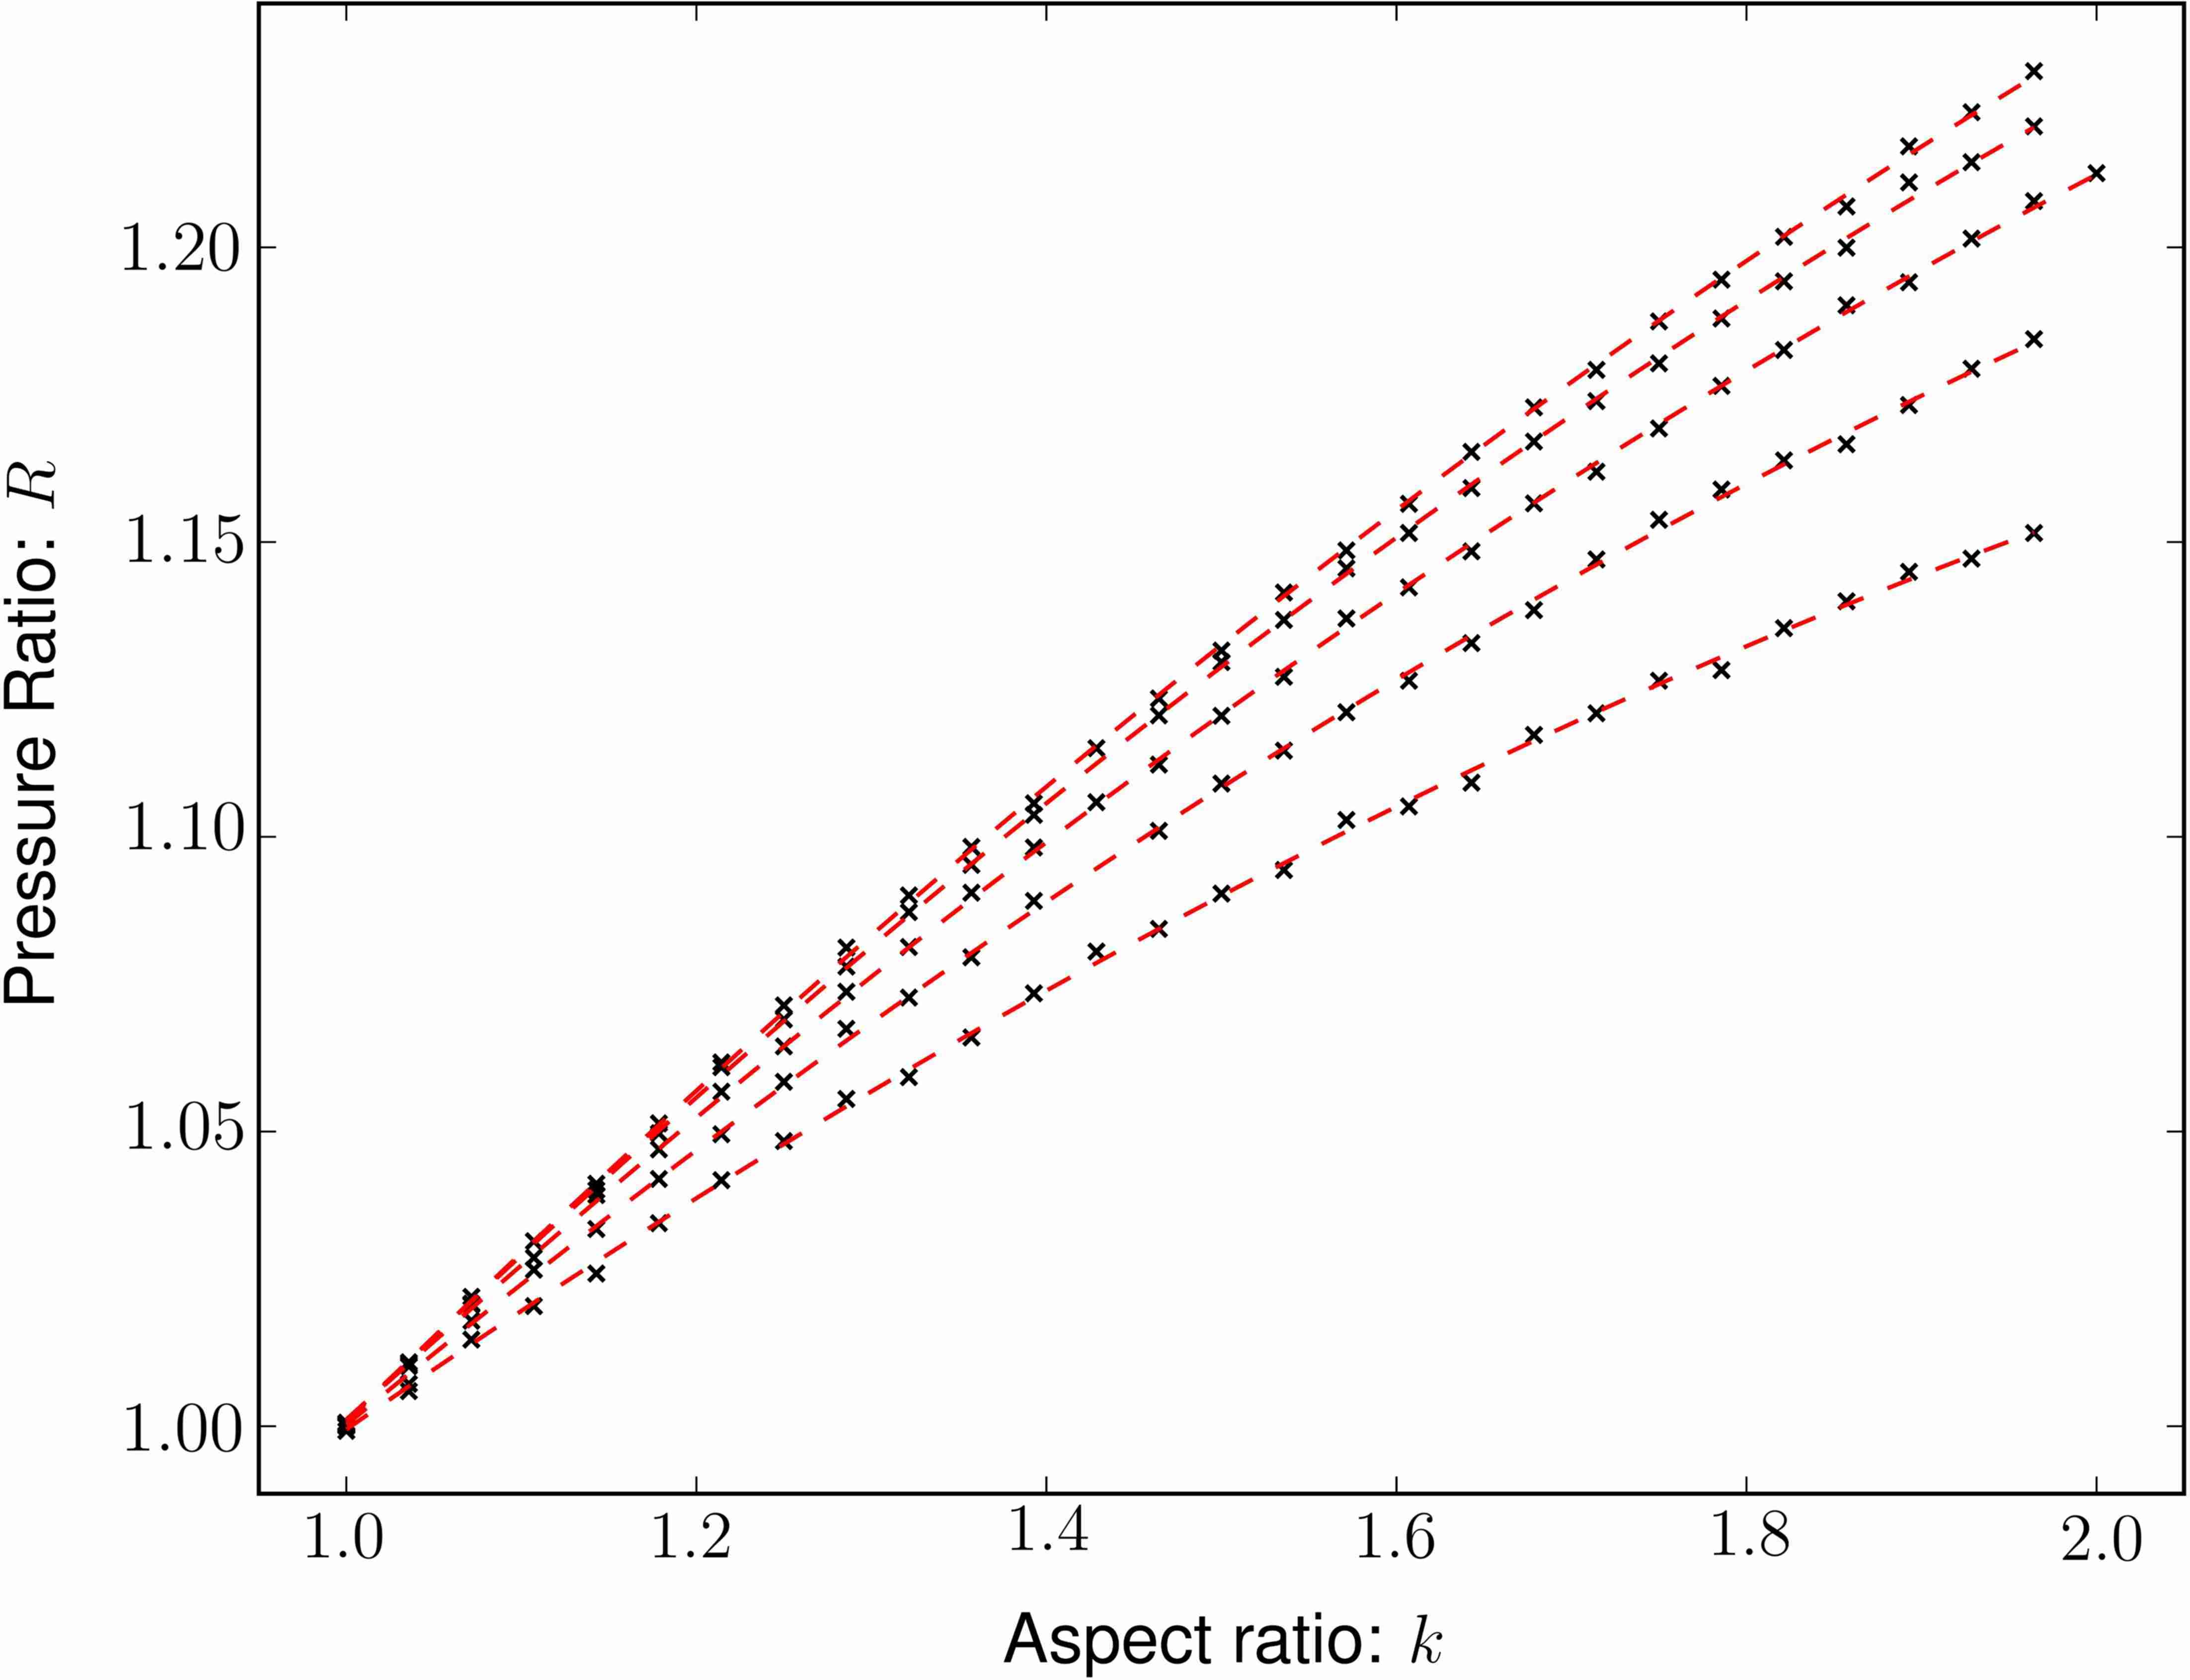
\includegraphics[width=\figurewidthSINGLE]{entropic_flow_paper/FIG4_EDIT.jpg}
\caption{Plot of the pressure ratio $R$ as a function of the aspect ratio $k$ for various values of fixed packing fraction $\Pi$. Each point on the graph represents a complete simulation with different parameters. The values of the fixed packing fraction include $\Pi=[0.10,0.15,0.20,0.25,0.30]$. A quadratic best fit curve shown for each value of $\Pi$ with the bottom curve corresponding to $\Pi=0.10$ and the other curves following sequentially. Note that each curve starts at $R=1.00$ regardless of $\Pi$ since the aspect ratio starts at $k=1.0$. }
\label{fig:Pratio_plot}
\end{figure}

\section{Theoretical Analysis}
As a first approximation, we consider an ideal crowder whose initial distribution is constant at $\rho$ and velocities are drawn from a Boltzmann distribution with temperature $T$. Under a hard-potential the angle of impact at the point of collision along the tangent surface is conserved. When a crowder particle impacts the boundary of the fixed ellipse the resulting trajectory conserves energy but not momentum. We define $\hat N(\phi)$ and $\hat T(\phi)$ to be the normal and tangent unit vectors from the parametrization of the ellipse
%
\begin{align}
\hat N(\phi) = g
\begin{bmatrix}
	E_b \cos \phi \\
	E_a \sin \phi \\
\end{bmatrix}  \\
\hat T(\phi) = g
\begin{bmatrix}
	E_a \sin \phi \\
	-E_b \cos \phi \\
\end{bmatrix}
\end{align}

The incoming and outgoing velocities $\vec v$, $\vec v'$ for are simply
%
\begin{equation}
\vec v' = \vec v - 2 \left ( \vec v \cdot \hat N(\phi) \right ) \hat N(\phi)  
\end{equation}
We can calculate the average angular momentum change for a given $\phi$ by rotating the incident velocity from $0^\circ$ to $180^\circ$ with respect to the tangent. In two dimensions, the cross product of any two vectors $\vec A, \vec B$ becomes a scalar quantity $\ell = \left[ \vec A \times \vec B \right]_{\hat z}=A_x B_y - B_x A_y$. We can define the scalar change of angular momentum with respect to the origin at the point $\vec Q(\phi)$ along the ellipse with incident velocity $\vec v$
%
\begin{align}
& \Delta \ell(\vec v, \phi) = \ell_f - \ell_i = \\
& \left [ \vec Q(\phi) \times \left ( \vec v - 2 \left ( \vec v \cdot \hat N(\phi) \right ) \hat N(\phi) \right ) \right ] _{\hat z} -
\left [\vec Q(\phi) \times \vec v \right ] _{\hat z} \notag
\end{align}

Assuming the crowder is uniformly incident from all angles, the average change in angular momentum at a given point along the ellipse can be found by direct integration of an incoming unit velocity vector
%
\begin{align}
\left < \Delta L(\phi) \right > = &\frac{1}{\pi} \int_0^{\pi} 
{\Delta \ell \left ( R(\theta)\hat T, \phi \right ) d \theta} 
\\
= &\frac{1}{\pi}
\frac
{-2(E_a^2-E_b^2) \cos \phi  \sin \phi }
{\sqrt{E_b^2 \cos^2 \phi - E_a^2 \cos^2 \phi + E_a^2}}
\notag
\end{align}
Where $\theta$ is the incident angle with respect to the tangent point of contact at $\phi$, and $R(\theta)$ is the rotation matrix
%
\begin{equation}
R(\theta) =
\begin{bmatrix} 
\cos \theta && -\sin\theta \\ 
\sin \theta &&  \cos\theta \\  \end{bmatrix}
\end{equation}

Lacking further information on the $\phi$ dependence of the velocity distribution we assume that this distribution is the same at all points. As such, an integration over a range of velocities drawn from a Boltzmann distribution at temperature $T$ would scale the expression by a constant factor. As expected, the expression reduces to $\left < \Delta L(\phi) \right >=0$ for circles. For aspect ratios where $k \neq 1$, we see in FIG. \ref{fig:delta_L} that there are four regions of non-zero $\left < \Delta L(\phi) \right >$ separated by the symmetries of the ellipse. If the crowder particles are allowed to interact, regions of alternating $\left < \Delta L(\phi) \right >$ indicate the potential to develop counter-rotating flows in each quadrant. 
%
\begin{figure}
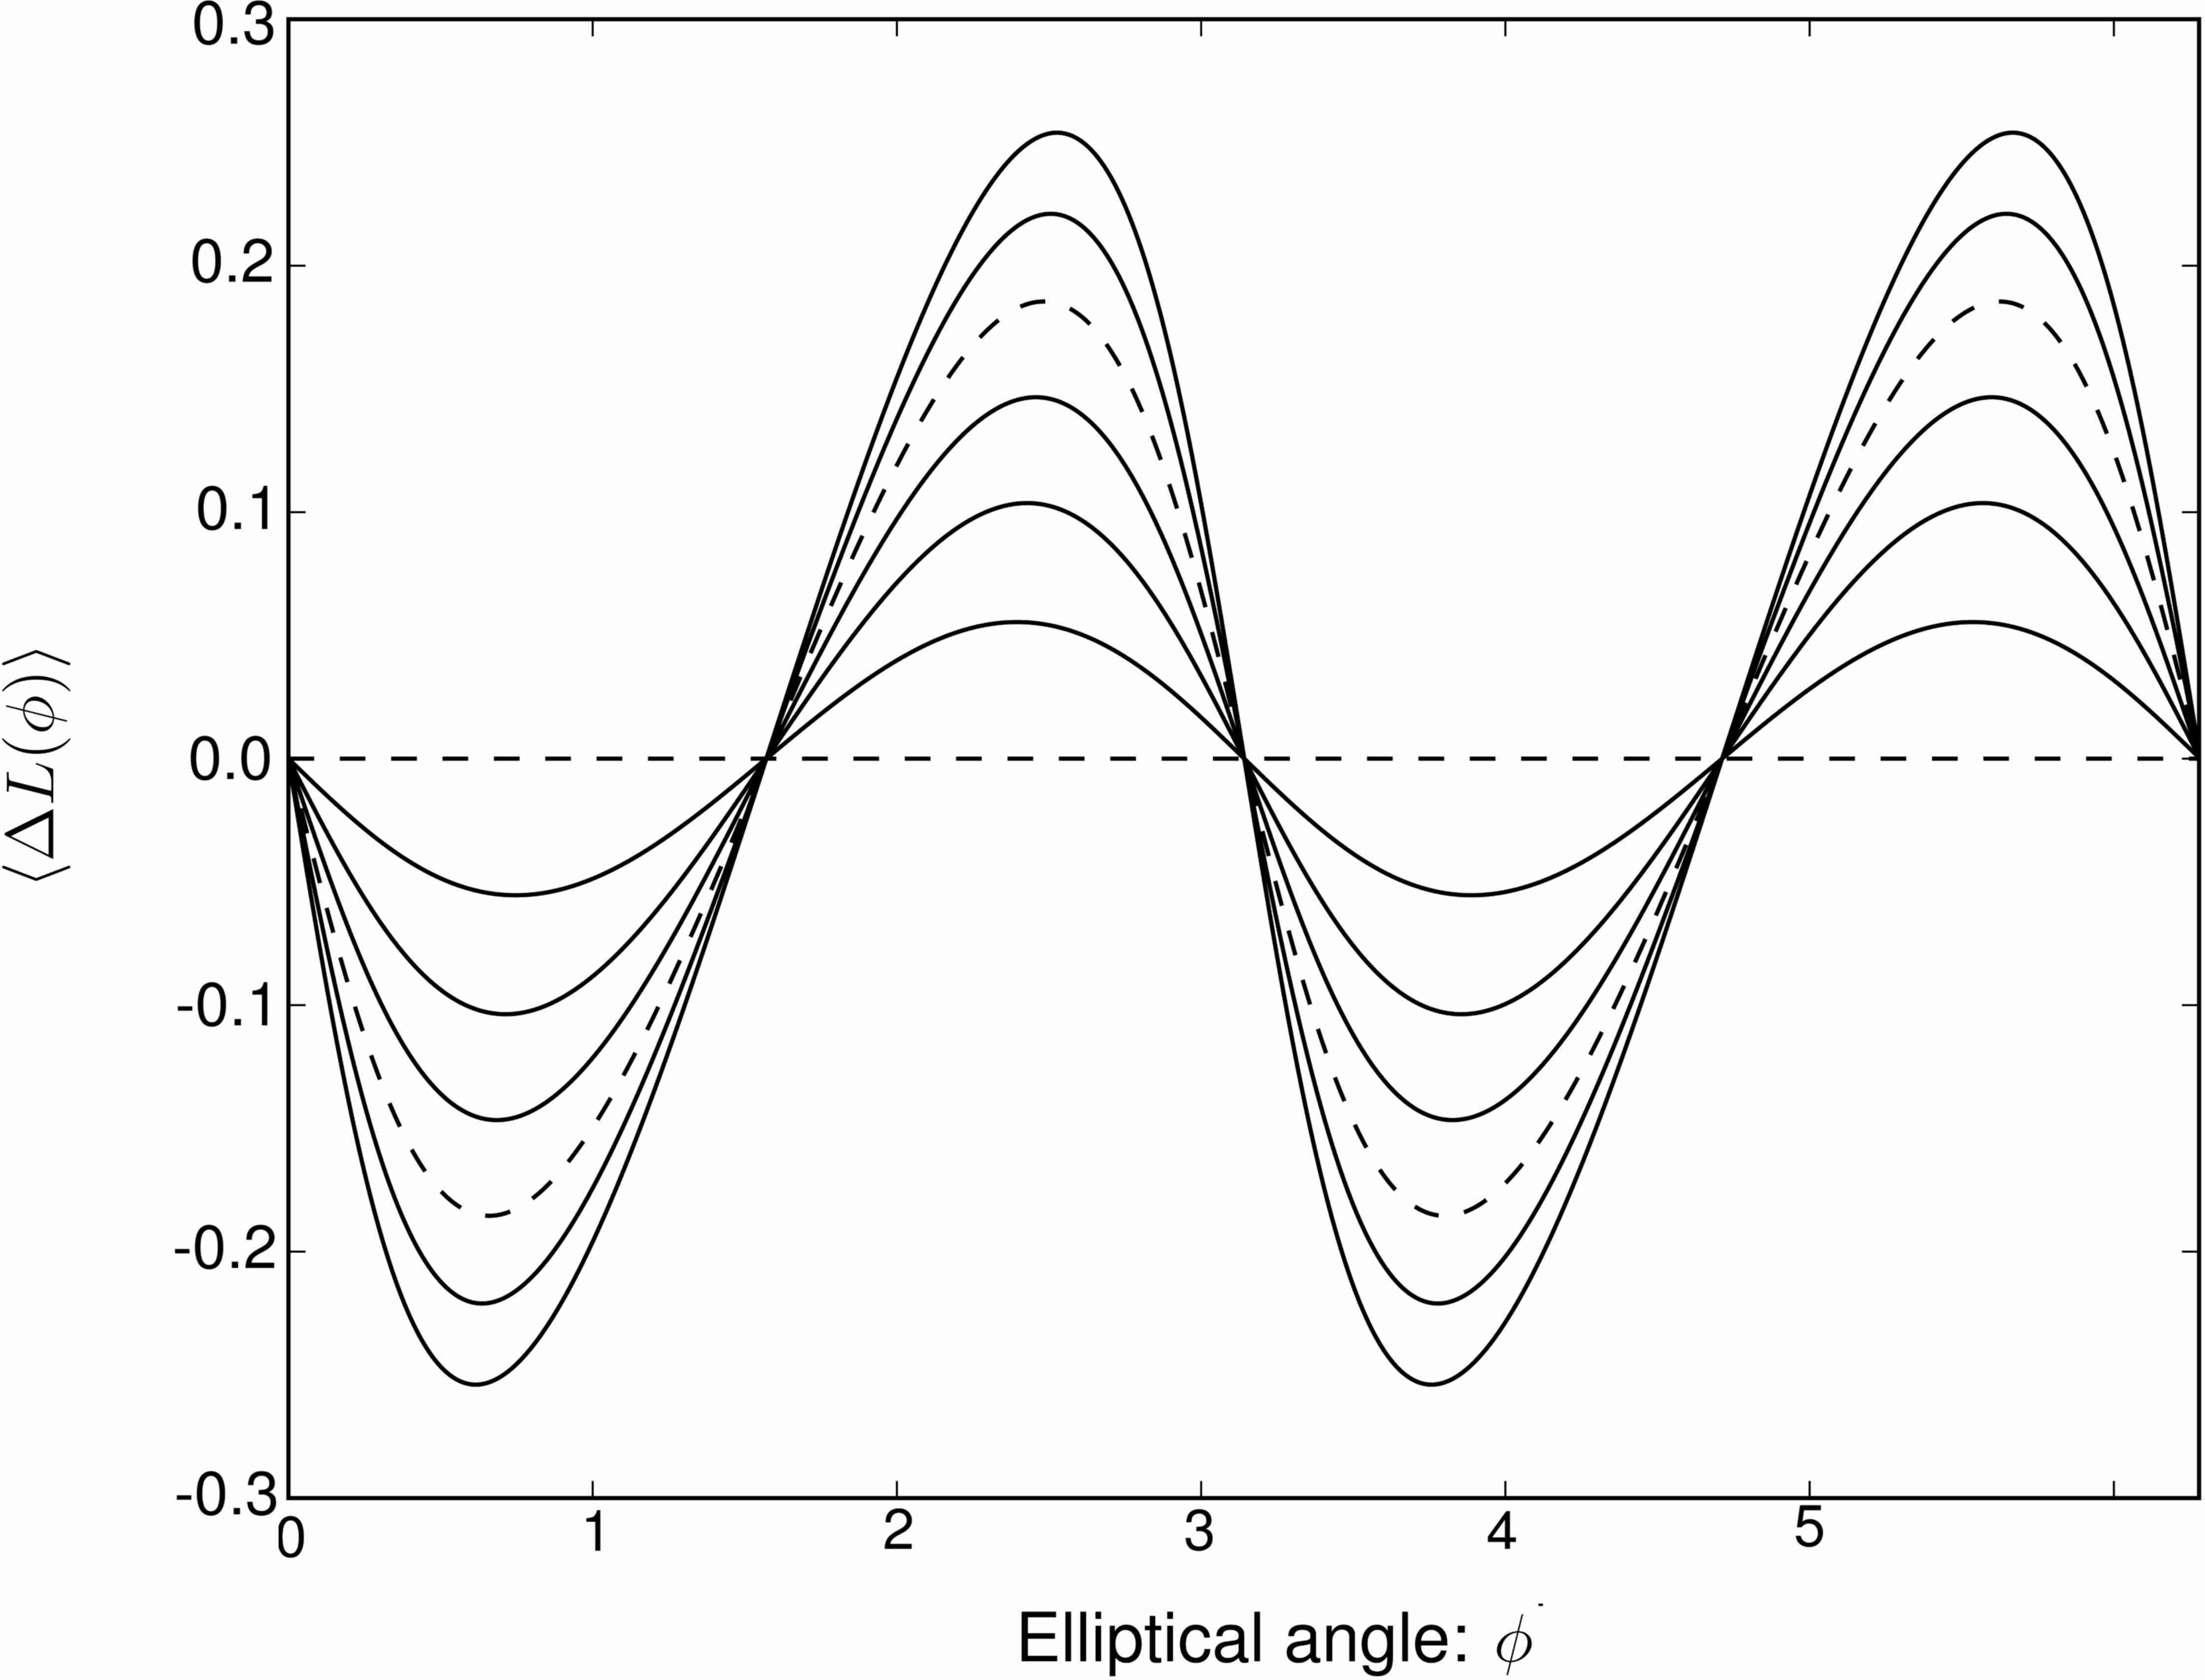
\includegraphics[width=\figurewidthSINGLE]{entropic_flow_paper/FIG5_EDIT.jpg}
\caption{Plot of $\left < \Delta L(\phi) \right >$ for various aspect ratios as a function of the elliptical parameter $\phi$. With area fixed at $E_a E_b \pi=1$, aspect ratios are plotted from $k=E_a/E_b=1$ to $k=2$ in increments of $1/6$. The dashed lines indicate the two curves $k=1,5/3$, with the flat line corresponding to the circle. }
\label{fig:delta_L}
\end{figure}
%
This approximation suffers from several drawbacks; an implicit assumption that the density is constant, that all impact angles $\theta$ have an equal probability, and the point-size radius of the crowders. However, this simplified calculation does suggest the fact that  vortex flow generation and the non-conservation of angular momentum of the system are related.

\section{Discussion}

Molecular dynamics simulations on the microscopic level have long been shown to exhibit behaviors on the macroscopic scale.\cite{rapaport_art_2004} In continuous systems where the flow is obstructed, the non-linear advective term $(\vec v \cdot \nabla) \vec v$ in the Navier-Stokes equation will convert linear momentum into angular momentum.\cite{hannon_molecular_1986} With a high enough Reynolds number, laminar flow around the obstruction becomes unstable and creates pairs of counter-rotating vortices. Theoretical calculations for flow past a sharp-edge plate predict some vortex formation at any non-zero Reynolds number.\cite{miyagi_standing_1983} The fact that vortices exist for any aspect ratio other than unity in our simulation agrees with these results, the difference here is that our system lacks any initial thermal, velocity or density gradients. 

The findings have important implications for all hard-potential models with curvature in the boundary conditions. Related to the original AFM experiment,\cite{yuan_effects_2008} the assumption that the protein has an elliptical shape leads naturally to the questions addressed in our experiment. Namely, does the addition of crowders induce shape changes for a fixed non-spherical molecule? The pressure ratio observed suggested that a return to a spherical shape, one that increased with both ellipticity and packing fraction. This effect is consistent with experimental observations\cite{yuan_effects_2008, homouz_crowded_2008} which show the tendency of macromolecules to return to a spherical shape at progressively higher packing fractions. In the context of the AFM experiment, our simulations agree that the presence of crowders led to a greater unfolding force required.

For the simulations of protein folding and unfolding processes, models of Brownian dynamics are often used. The equivalence of Brownian and hard-disc dynamics has been previously investigated in the literature.\cite{hofling_critical_2008, gleim_relaxation_1998} In a hard-potential simulation all particles maintain an infinite memory of their previous trajectories. Contrast this with the Langevin dynamics which include a viscous damping term along with a random component. In these dynamics the particles maintain only a partial memory of their previous trajectories. In the current simulation, reducing the memory of the particles (by including a viscous drag and random force component) reduces the effect the elliptical boundary condition has on the surrounding environment. In the extreme case of Brownian motion, the density profiles extend only as far as the Brownian steps themselves.  

The point of the above observation is to highlight a crucial difference between hard-sphere simulations with and without memory. The distinction may be irrelevant for a rarefied hard-sphere gas such as argon, but may play a role in the crowded molecular environment. While the role of memory (or lack thereof) in biological simulations is important, we feel that the conclusions drawn from these simulations are still applicable. To the extent that DMD and Brownian dynamics are equivalent, our result can be used to explain both the AFM and shape change experiments.



  %CHAPTER: Conformational States Under Crowding
  \chapter{Conformational States Under Crowding}
\label{chap:WL_crowding}

\section{Experimental Motivation \label{sec:intro}}

The idealization of dilute conditions in conventional \textit{in vitro} biophysical experiments has long been recognized to ignore the important aspect of crowding. In typical cellular environments, the experimental, computational, and theoretical results have shown crowding agents to affect the stability of proteins and the rates of protein folding. The measured and predicted effects of crowding, however, are varied and seem to be dependent on both the protein and the crowders themselves. For a summary of the recent developments in the field since 2004, see the excellent review by Zhou, Rivas and Minton.\cite{zhou_macromolecular_2008} Crowding effects are still actively being explored, with most efforts focusing on the entropic effects to elucidate the response common to all crowding agents. While energetic interactions may exist between the protein and the crowding agents, a simplified yet effective treatment of a crowder is that of a steric, inert particle, affecting the entropy of the protein's conformational state according to its compactness and shape.\cite{hoppe_entropic_2009, homouz_crowded_2008}

In one limit, where the crowding particles are much larger in volume and mass than the protein, good results have been obtained by approximating the crowders through localization. Typically this is modeled as confinement between parallel plates, or in spherical or cylindrical cavities.\cite{mittal_thermodynamics_2008, wang_confinement_2009, zhou_stabilization_2001} In these approximations, the conformations that are extended beyond the confinement wall are excluded. In the other limit, where the crowders approach the size of a typical residue, the effects of excluded volume dominate. Here, not only are the extended conformal states of the protein highly perturbed, but intermediate states are also proportionally less favored to those states that are compact.\cite{minton_effect_2000}

In this chapter, we investigate the effects of crowders on the folding properties of $\beta$-sheet proteins using a lattice model. While lattice-based approaches are numerous, those that connect their results to physical experiments are less so. We are motivated by the experiments done by Gai and coworkers\cite{xu_probing_2008, mukherjee_effect_2009,du_understanding_2006} and examine our model in light of their observations. We recognize however, that simple lattice-bead models capture only a portion of the conformational entropy; typically only the gross features of the backbone are correctly modeled. To accommodate for the orientational entropy of the dihedral or $\phi$-$\psi$ angles, we introduce an Ising-like model. Each bead along the chain is associated with a binary internal state, with an interaction potential requiring the energetic contributions of two beads to have the same state. Since the correct configuration of the dihedral angles is essential for proper hydrogen-bond formations, this extra degree of freedom gives a physically motivated Hamiltonian that implicitly includes the hydrogen-bond contacts. We model the positional entropy of the backbone by projecting it onto a face-centered cubic (fcc) lattice. We use a $\Go$-like Hamiltonian to model the native connections and to ensure the existence of a unique ground state. With the conformational entropy defined we propose a model that attempts to capture the salient aspects of macro-molecular crowding using a detailed density of states (DOS) calculation. 

Once the DOS has been determined, we use the results of the scaled particle theory (SPT) to approximate the effects of crowding on several $\beta$-sheet proteins. The use of the SPT to study the conformational states of the protein folding process is, of course, not new and has been studied previously, see~\cite{mittal_dependence_2010, ping_depletion_2006, batra_effect_2009, minton_models_2005} and the references cited therein. We model the protein as right circular cylinder since the native state of $\beta$-sheets are naturally disk-like. The crowders, Ficoll 70, are modeled as sphereocylinders accounting for their observed elongation.\cite{asgeirsson_glomerular_2007, fodeke_quantitative_2010} Our treatment is unique among the previous studies in that we use the Wang-Landau algorithm to determine density of states for the positional and orientational entropies, separately. This gives us an accurate measurement of the crowding effects across the conformations of the density of states and the ability to compute thermodynamic quantities to high accuracy.

The organization of this chapter is as follows. In Section \ref{sec:methods} we introduce the Hamiltonian and the effective free energies associated with crowding and the dihedral angles. In this section, we explicitly define the cost, both enthalpically and entropically for each conformation. We demonstrate how the density of states can be factored into two terms, greatly speeding up the calculation using the Wang-Landau algorithm. We then describe the experimental results in Section \ref{sec:results} and fit our model to the experimental observations. We use the SPT to determine the effect of crowders on the thermodynamic quantities and discuss the implications. Finally, we use the results to make predictions for future experiments.

\section{Methods \label{sec:methods}}

Our protein is coarse grained to a chain of beads and projected as a self-avoiding walk onto a fcc lattice, with a `bead' representing an amino acid residue. The fcc lattice was chosen over the traditional cubic lattice to provide more degrees of freedom. Previous works have found the fcc lattice to be a more natural fit to the secondary structures of $\alpha$-helices and $\beta$-sheets.\cite{peto_generation_2007, pokarowski_minimal_2003} The choice of lattice is not arbitrary, as higher coordination numbers and different symmetries may better represent the underlying structure. For a summary on the effect of lattice choice see Pierri \textit{et al}.\cite{pierri_lattices_2008}

Two beads are considered nearest-neighbors if they are on adjacent sites on the lattice. With the underlying lattice being defined by a set of primitive vectors $\B{e}$, we define two lattice points $\mathbf{x}_i, \mathbf{x}_j$ to be nearest neighbors iff there exists a vector $\mathbf{v} \in \B{e}$ such that $\mathbf{x}_i =  \mathbf{x}_j + \mathbf{v}$. For convenience, we define the twelve lattice steps in Cartesian coordinate space $(x,y,z)$ that form the base set of a face-centered cubic lattice
\begin{equation*}
\B{e} = l
\brackets{
\begin{array}{rrrrrrrrrrrr}
1&1&1&1&0&0&0&0&-1&-1&-1&-1\\
1&-1&0&0&1&1&-1&-1&0&0&1&-1\\
0&0&1&-1&1&-1&1&-1&1&-1&0&0
\end{array}
}
\end{equation*}
%
These twelve vectors define the nearest-neighbors for a given lattice point. Here $l=3.8$\AA  \hspace{.2em} is the length scale of the lattice, which is the average spacing between two C$_\alpha$ atoms. Let the set of all backbone conformations be denoted by $\mathcal{C}$ with the vector $\mathbf{c} \in \mathcal{C}$ representing an individual conformation on the lattice. 

Our model Hamiltonian is a modification of the $\Go$-model,\cite{abe_noninteracting_1981} where the only energetic contributions are either from the attraction of the residues that are predefined native contacts or the repulsion of the nonnative ones. The $\Go$ model, primarily a model of minimal frustration, typically ignores the potential from non-native contacts. Models with the repulsive terms added,\cite{knotts_iv_entropic_2008, hoang_molecular_2000} create a frustrated energy landscape since more structural information is encoded in the Hamiltonian. In addition, the high coordination number of the fcc lattice does not always admit a unique native state for some structures without the nonnative term. We let $\GO$ be a symmetric matrix of native contacts, $\GO_{ij}=1$ iff positions $i$ and $j$ are native contacts of the protein, otherwise $\GO_{ij}=0$.  

In addition to the $\Go$-like native contacts we further require that the beads have the correct orientations. To achieve this, each bead has a binary internal state, representing the correct (or incorrect) range of values of its dihedral angles. This is similar to the ideas presented in the Mu{\~n}oz-Eaton (ME) model\cite{munoz_simple_1999} where each amino acid is allowed two internal states, folded or unfolded. While ME model has been solved exactly in a restricted form\cite{bruscolini_exact_2002} and incorporated into more extensive models,\cite{chung_temperature-dependent_2008} we exploit the fact that the ME model generates a density of internal states that is easily decoupled with the positional microstates, thus leading to more precise estimate of the thermodynamic variables. The permutations of these internal states generate an ensemble of microstates; let the set of all such state sequences be denoted $\mathcal{S}$, with the vector $\mathbf{s} \in \mathcal{S}$ representing a particular sequence of the internal states. It will be useful to refer to the total number of folded beads for a state $\sigma = \sum_{i=1}^{L} \mathbf{s}_i$, with the unfolded/folded states defined, indexed by $s_i=0 / s_i=1 $, and amino acid residue count $L$.
 
Our Hamiltonian depends on the number of native and non-native contacts of all the beads on the lattice and on their internal state
\begin{equation}
\mathcal{H}(\mathbf{c},\mathbf{s}) = 
- \sum_{i=1}^L \sum_{j=i+2}^L 
\omega_{ij} [ J_+ \mathbf{s}_i \mathbf{s}_j  \GO_{ij} - J_- (1 - \GO_{ij}) ],
\end{equation}
where $\omega_{ij}=1$ iff residues $i$ and $j$ are nearest-neighbors on the lattice and $J_{+}$, $J_{-}$ represent the strength of the $\Go$ model's native and non-native contacts, respectively. A more intuitive form can be written by counting the number of contributions from the native $\KP$ and non-native $\KM$ contacts:
\begin{align}
\label{eq:Hamiltonian}
\mathcal{H}(\mathbf{c},\mathbf{s}) &= -J_+ \KP + J_- \KM  \\ \nonumber
\KP &= \sum_{i=1}^L \sum_{j=i+2}^L \omega_{ij} \mathbf{s}_i \mathbf{s}_j  \GO_{ij} \\ \nonumber
\KM &= \sum_{i=1}^L \sum_{j=i+2}^L \omega_{ij} (1 - \GO_{ij}) 
\end{align}

There are two entropic effects incorporated into the free energy, the crowding and the dihedral angle restrictions. The free energy of a state $(\mathbf{c}, \mathbf{s})$ is
\begin{equation}
\mathcal{F}(\mathbf{c},\mathbf{s}) = \mathcal{H}(\mathbf{c},\mathbf{s})  - \beta \Delta \psi(\sigma) - \beta \Delta \mu(\mathbf{c})
\label{eq:free_energy}
.
\end{equation}
Here $\beta=1/k_B T$, $\beta \Delta \psi(\sigma)$ is the free energy term  associated with the entropy of the dihedral angle orientation and $\beta \Delta \mu(\mathbf{c})$ is an entropic cost of inserting the protein into a solution of crowders (both terms to be defined in later sections). By modeling the crowders implicitly as hard-particles there is only entropic cost for insertion, the term is truly a free energy contribution. If however, the crowder specifically interacts with the protein this contribution must be included in the Hamiltonian. The model admits three fitting parameters $(J_+, J_-, h)$, with $h$ setting the energy scale of the dihedral angle term $\beta \Delta \psi(\sigma)$. Additionally, the crowding term $\beta \Delta \mu(\mathbf{c})$, depends on the concentration and the geometry of the crowders.

The positional conformation $\mathbf{c}$ determines the number of non-native contacts $\KM$, thus we take $\Omega(\mathbf{c},\sigma, \KP)$ as the density of states. The partition function can be factored by summing up to the maximum number of native contacts $\KPMAX$:

\begin{align}
\mathcal{Z} 
    &= \sum_{\mathbf{c} \in \mathcal {C}}  \sum_{\mathbf{s} \in \mathcal {S}} 
            e^{-\beta \mathcal{F}(\mathbf{c},\mathbf{s})} \\ \notag 
    &= \sum_{\mathbf{c} \in \mathcal {C}}  \sum_{\sigma = 0}^{L} \sum_{\KP = 0}^{\KPMAX} \Big [
             \Omega(\mathbf{c},\sigma, \KP) e^{ \beta \Delta \psi(\sigma) + \beta \Delta \mu(\mathbf{c}) } 
      \sum_{\mathbf{s} \in \mathcal {S}, \Sigma {\mathbf{s}_i}=\sigma }  
            e^{-\beta \mathcal{H}(\mathbf{c},\mathbf{s})} \Big ] \notag
\end{align}


\subsection{Conformational Entropy of Dihedral Angles}

Associating an entropic cost with the correct dihedral angles is an idea that goes back to the original Zimm-Bragg (ZB) \cite{zimm_theory_1959} and Lifson-Roig (LR) models.\cite{lifson_theory_1961} These models were first used for helix-coil transitions, and later extended to include sheets.\cite{mattice_matrix_1984, hong_statistical_2008, schreck_exactly_2010} Letting each bead have an internal state, native or non-native, allows us to capture some of the detail present in more complex models, yet still retain the simplicity inherent in lattice models. It is the lack of spatial degrees of freedom that separate the ZR, LR type models from the one presented here. In our model each conformation defines a new Ising-like sub-problem, where we consider the entropy associated with the ensemble of `spins' of only the nearest neighbor contacts. 
Our model is actually the generalized variant of the spin systems, commonly referred to as the Potts model. There are two major distinctions between the Ising and Potts models; the spin directions are not necessarily restricted to two states and the strength of spins in contact are determined by an interaction matrix. We still retain the two state model, folded/unfolded, but our interaction matrix has only a single non-zero term, contributing only when both spins are in the folded state. This is evident by the $\mathbf{s}_i \mathbf{s}_j$ term in the Hamiltonian since $\mathbf{s}_i, \mathbf{s}_j \in \{0,1\}$. However, each folded residue comes at a price, the entropic cost of restricted dihedral angles for a single bead is
\begin{equation}
\beta \Delta \psi(\sigma) = h \sum_{i=1}^L \mathbf{s}_i = h \sigma
.
\end{equation}

\subsection{Reduction of State Space - Conformational Decoupling}

Since the Hamiltonian, and thus the free-energy, is a function of both positional conformations $\mathbf{c}$, and the orientational conformations  $\sigma, \, \KP$, it would seem that a calculation of the full density of states $\Omega(\mathbf{c},\sigma, \KP)$, is necessary. We will show however, that given a positional conformation, one can decouple the internal states by grouping similar conformations into isomorphic macrostates. Consider the matrix
\begin{equation}
\CHIX_{ij} (\mathbf{c}) = \GO_{ij} \omega_{ij} (\mathbf{c})
\end{equation}
of the positive energetic contributions to the Hamiltonian when one ignores the internal states. We can map this symmetric matrix to a simple, but possibly disjoint graph, $\CHIX_{ij} \rightarrow g(\mathbf{c})$, by observing that $\CHIX$ is an adjacency matrix. Let $\text{Aut}(g(\mathbf{c}))$ define the automorphism group to which $\mathbf{c}$ belongs. Each $\text{Aut}(g(\mathbf{c}))$ is a permutation group, whose members are related by mapping the vertices of the graph onto itself through permutation such that the resulting graph is isomorphic to the original. While all graphs in the same automorphism group are isomorphic to each other, we should note that not every graph is physically realizable in our lattice model due to the restriction that no two beads can occupy the same lattice site. The key to decomposing the density of states, however, is the grouping of the graphs, and hence the conformations. Each automorphism group defines a finite-graph for a spin-state system. The density of states for this finite-graph system is calculated by considering, over all possible `spins' of the system, the restricted counts of $\sigma$ and $\KP$. Since the problem of finding the internal states is identical for all members of a particular automorphism group we can decouple the density of states as
\begin{equation}
\Omega(\mathbf{c}, \sigma, \KP) = \Omega_1 (\mathbf{c}) \, \Omega_2 (\sigma, \KP; \CHIX(\mathbf{c}))
\end{equation}

As an illustrative example of the decoupling method consider a 12 bead homopolymer defined over a cubic lattice where every connection is favorable ($\GO_{ij} = 1$ if $|i-j| > 1$) in the particular conformation shown in Figure \ref{fig:Sample_homopoly_backbone}. All of the native connections, which in this case are simply all nearest neighbors, are shown in Figure \ref{fig:Sample_homopoly_connections}. Abstracting the representation to a graph in Figure \ref{fig:Sample_homopoly_graph} shows the finite system that solves the density of states over the Potts model. Usually, when solving a Potts/Ising-type system the underlying graph has a high degree of symmetry (cubic lattices or Cayley trees are common examples). For a typical graph produced by our model this symmetry is broken, forcing us to numerically compute $\Omega_2 (\sigma, \KP; \CHIX(\mathbf{c}))$. However, the number of edges in the graph determine the maximum number of favorable connections. Since this number is small, the convergence of the Wang-Landau algorithm on this portion of the DOS is rapid.
\begin{figure}[ht]
  \subfloat[][Backbone $\mathbf{c}$]{\label{fig:Sample_homopoly_backbone}
 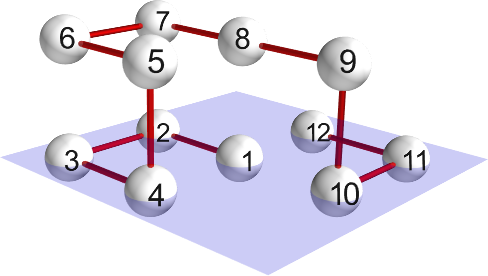
\includegraphics[width=\figurewidthTRIPLE]{WL_crowding_paper/homopoly_backbone_trim.png}}
 \subfloat[][Native Contacts $\CHIX(\mathbf{c})$]{\label{fig:Sample_homopoly_connections}
 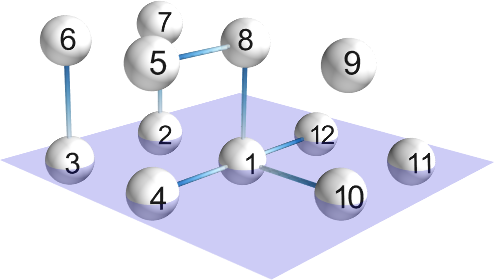
\includegraphics[width=\figurewidthTRIPLE]{WL_crowding_paper/homopoly_connections_trim.png}} \\
 \subfloat[][Connection Graph $\CHIX(\mathbf{c}) \to g(\mathbf{c})$]{\label{fig:Sample_homopoly_graph}
 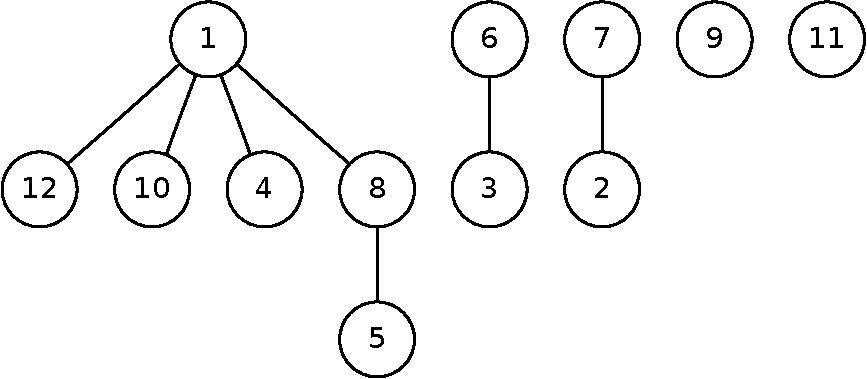
\includegraphics[width=\figurewidthSINGLE]{WL_crowding_paper/3d_example_graph-crop.pdf}}
\caption{Sample homopolymer (with all connections favorable) on a cubic lattice with (a) the backbone, and (b) the energetically favorable connections. The problem of finding the density of states for the internal conformations of each bead for this conformation is then reduced to solving the density of states of the Potts model over the graph shown in (c). Note that the labels in (c) are shown only to guide the eye, all valid permutations of the indices belong to $\text{Aut}( g(\mathbf{c}) )$ and hence define the same Potts sub-problem. The $\GO$ model in the Hamiltonian would make some of the connections in $\CHIX(\mathbf{c})$ unfavorable, further simplifying the problem. Additionally, our model is defined over a fcc lattice, while the example shown above is a cubic lattice for illustrative purposes.}
\end{figure}

In general, grouping a particular $\mathbf{c}$ to its automorphism group requires solving the graph isomorphism problem multiple times. While specialized algorithms exist,\cite{mckay_practical_1981} the computational solution is unique in its complexity class and lacks a simple invariant that definitively determines isomorphism.\cite{kaebler_graph_1993} The problem is greatly simplified if the energetic matrix $\GO$ permits only a few, highly degenerate sets of graphs. The Hamiltonian defined for $\beta$-sheets happens to be one of these favorable partitions. Since the $\beta$-sheet structure is essentially planar, moving perpendicular to the strand direction identifies a column of connections. When abstracted to a graph, the only structure possible is that of a linear chain (unary tree), whose length is limited by the number of strands. The set of conformations $\mathcal{C}$ for $\beta$-sheets create graph structures that have a high degeneracy and consequently low cardinality in the set of unique automorphism groups. Additionally, checking for graph isomorphism of linear chains is trivial since these graphs can be uniquely determined by a single number, the chain length. These two facts combined significantly speed the computation of the decoupled density of states $\Omega_1 (\mathbf{c}) \Omega_2 (\sigma, \KP; \CHIX(\mathbf{c}))$.

\subsection{Implicit Crowding Effects}
We study the effects of crowders to our protein system using the scaled particle theory. In one of the original formulations of SPT~\cite{lebowitz_scaled_1965} one calculates the work done to expand a spherical cavity of radius $R$ in a hard sphere fluid of radius $r_c$. The centers of the fluid particles are excluded from the cavity region, which implies that meaningful values of $R$ must be greater than $-r_c$. This work $W(R)$ is the configurational part of the chemical potential for a single solute particle $\Delta \mu (\mathbf{c}(R))$. The relationship between the probability of any particular configuration and the work required to create it is $P(R) = \exp( - \beta \Delta W(R))$, where $P(R)$ is the probability that there are no centers of fluid particles of radius $r_c$ in the spherical region $(R+r_c)$. If we approximate both our protein and crowders as hard-spheres, we can calculate the work required to create the proper cavity. One first calculates the probability of finding a cavity whose size can accommodate only a single spherical solute particle. This yields 
\begin{equation}
W(-r_c\!\leq R\!\leq 0) = -kT \ln(1- (4/3) \pi \eta (R+r_c)^3)
,
\end{equation} 
where $\eta$ is the number density of the solvent. One expands $W(R)$ around $R=0$ to the second order (noting that the leading term for large $R$ must be the pressure-volume term $4/3 \pi p R^3$ with $p$ as the pressure of the fluid) and obtains 
\begin{eqnarray}
\beta \Delta \mu (\mathbf{c}(R)) = &
\beta( \Delta \mu (\mathbf{c}(0)) 
 + \Delta \mu ^\prime(\mathbf{c}(0)) R \\ \nonumber &
 + \frac{1}{2} \Delta \mu  ^{\prime \prime}(\mathbf{c}(0)) R^2 
 + \frac{4}{3}\pi p R^3 )
\end{eqnarray}
These terms can be computed by the continuity of $W(R)$ and its first two derivatives at $R=0$. The pressure can be found by substituting in the exact solution of the Percus-Yevick equation, yielding a density approximation as a function of the packing fraction $\phi$. This density route is not unique among thermodynamic pathways. Expressions have been worked out for both compressibility and viral routes.\cite{chen_different_2003} Each of these pathways amount to a smoothing in the structural information of the fluid as one `turns-on' the density field. The compressibility and viral routes tend to yield better approximations to the solvation free energy, giving
\begin{eqnarray}
(\beta \Delta \mu)_\text{spherical}  &=&
\frac{\phi(-2+7\phi-11\phi^2)}{2(1-\phi)^3} 
- \ln(1-\phi) 
\\ \nonumber & &
+ \frac{18\phi^3}{(1-\phi)^3} \paren{ \frac{R}{2r_c} }
- \frac{18\phi^2(1+\phi)}{(1-\phi)^3} \paren{ \frac{R}{2r_c} } ^ 2 \nonumber
\\ \nonumber & &
+ \frac{8\phi(1+\phi+\phi^2)}{(1-\phi)^3} \paren{ \frac{R}{2r_c} } ^3 
\label{eq:SPTcrowders}
\end{eqnarray}

The above treatment by SPT assumes, however, that the cavity created is spherical, a condition that is not rigorously satisfied for the crowders nor the proteins examined in this study. The native states of the proteins studied in this work can be well approximated by a right circular cylinder, as the $\beta$-sheet structures are disk-like. Additionally our crowder, Ficoll 70, is known to have an elongated shape \cite{asgeirsson_glomerular_2007} and recent predictions\cite{fodeke_quantitative_2010} model them as sphereocylinders with diameter of 28 \AA\ and an end-to-end length of 184 \AA. The extension of SPT to work with aspherical mixtures can be expressed through the activity coefficient.\cite{boublik_statistical_1974, minton_molecular_1998} The activity coefficient $\gamma_i$ is the measure of the deviation of the ith species at the actual composition of the solution from the chemical potential of an ideal solution as given by the equation,
\begin{equation}
\label{eq:mu_i}
RT \ln{\gamma_i} \equiv \mu_i - \mu_i^{0}
\end{equation}
where $\mu_i^0$ is the chemical potential of a reference state. For hard-convex particles the non-ideality of a particular species of interest can be found by computing an expression as a function of the volume $V_i$, surface area $S_i$ and the Kihara support function $H_i$ of that species,\cite{fodeke_quantitative_2010} given by
\begin{eqnarray}
\label{eq:gamma_i}
\ln{\gamma_i} &= -\ln(1-\avg{V}) 
+ \frac{H_i \avg{S} + S_i\avg{H} + V_i\avg{1}}{1-\avg{V}} \\
&+ \frac{H_i^2 \avg{S}^2 + 2 V_i \avg{H}\avg{S}}{2(1-\avg{V})^2}
+ \frac{V_i \avg{H^2}\avg{S}^2 }{3(1-\avg{V})^3} \nonumber
,
\end{eqnarray}
where $\avg{X} \equiv \Sigma \rho_i X_i$ and $\avg{1} \equiv \Sigma \rho_i$ are the averages over the different species, with $\rho_i$ as the number density of that species. For a right circular cylinder and sphereocylinder respectively the Kihara support functions are $H_\text{\text{sphereocylin}} = r\pi/4 + L/2$ and $H_{\text{cylinder}} = r + L/4$ with $r$ as the radius and $L$ as the length of the cylindrical section. 

In the process of calculating the density of states, we can sample the conformations to determine the parameters for the activity coefficient. For each conformation of the peptide we calculate a best fit circular cylinder by pointing the axis of the cylinder along the largest principle axis of the bead positions then scale the radius and length so all beads fit inside. Using Eq. \ref{eq:mu_i} and \ref{eq:gamma_i} we can determine the free energy due to crowders in our system.


\subsection{Implementation of the Wang-Landau Method}

For a review of the Wang-Landau method and a definition of the terms see Chapter \ref{sec:wang_landau}. All of the computations carried out in this chapter took $f_0 = e^{1} \approx 2.71828$, $f_{\text{final}}= e^{-9}$, and $f_{i+1} = \sqrt{ f_{i} }$. Each time a conformation was selected, the DOS is updated along with a histogram of visits for that conformation $H(\xi)$. The factor $f$ was reduced when $H(\xi)$ was no less then $90\%$ of the average number of visits for all conformations $\avg{H}$. Once the factor $f$ had been reduced we reset the histogram of visits for all conformations, $H(\xi)=0$, and began the process again. Each conformation is still directly related to a numerical energy. By calculating the DOS for conformations we can delay the calculation of the energy. This has the advantage that multiple simulations are not required for each set of the system parameters $(J_+, J_-, h, \phi, r_c)$.

Our move set consists of pull moves, which were first defined over a cubic lattice \cite{lesh_complete_2003} and later for triangular lattice models.\cite{bockenhauer_local_2008} Pull moves are an ergodic, reversible move set that modify the positional conformations by moving the chain along a path defined by a pair of beads adjacent in chain sequence $(i, i+1)$. Since the number of moves are finite and easily computable, we can quickly determine the factors necessary for detailed balance (i.e.\ $n_A$, $n_{A \to B}$, etc).

When converged, the WL method gives a flat histogram. That is, the averaged fraction of time spent at each macrostate approaches the same constant. Here we define a macrostate as the set of all conformations with the same energy level. Not every microstate is visited during the simulation, nor would it be possible due to the exponential growth in the DOS as a function of chain length. We assume that the visits to each state are ergodic, subsequent visits to a macrostate will visit each conformation an equal number of times over long averages. This idea is reasonable when we consider detailed balance is obeyed for the Monte-Carlo simulation, and is employed by Wust and Landau.\cite{wust_versatile_2009} We exploit this observation to determine a probability distribution for a second observable as a function of the first. For instance, we can step through the conformations to compute the probability distribution of the activity coefficient for the protein in a particular conformation $\mathbf{c}$. Doing so prevents the need for a multiplicative increase in the density of states (thus speeding up the convergence of the WL algorithm), yet it still provides us with a reasonable estimate of an extended DOS $\Omega(\mathbf{c}, r_g)$.

\section{Results 
\label{sec:results}}

\subsection{Model Calibration}

Unlike $\alpha$-helices, the $\beta$-sheet motif has been difficult to study experimentally due to its propensity to aggregate. Recently there has been a spate of designed peptides that exhibit the $\beta$-sheet motif, albeit with extremely broad thermal transitions.\cite{cochran_tryptophan_2001} We consider and describe below, three experimentally designed $\beta$-sheets peptides used in this study. These designed proteins were specifically chosen to test the model against their readily available experimental measurements. 

The first peptide (sequence: \texttt{RFSEV$^D$[PG]\linebreak[0]KKFITS$^D$[PG]\linebreak[0]KTYTEV$^D$[PG]\linebreak[0]KKILQ}, nicknamed $^D$P$^D$P$^D$P) is a 28-residue chain with a natural four strand $\beta$-sheet structure. This designed peptide was studied experimentally by Xu \textit{et.\ al.\ }~\cite{xu_probing_2008} as an extension of the peptide $^D$P$^D$P-II first proposed by Gellman and co-workers.\cite{syud_influence_2003} A schematic model of the native state for the peptide is shown in Figure \ref{fig:28_residue_seq_chem_sch}. The second peptide (sequence: \texttt{RFIEV$^D$[PG]\linebreak[0]KKFITS$^D$[PG]\linebreak[0]KTYTE}, nicknamed $^D$P$^D$P) is a 20-residue chain with a natural three strand $\beta$-sheet secondary structure.\cite{hudson_measuring_2006} The final peptide (seq: \texttt{GEWTWAD[AT]\linebreak[0]KTWTWTE}, nicknamed trpzip4-m1), is a 16-residue variant of the tryptophan zippers studied by Cochran \textit{et.\ al.\ }\cite{cochran_tryptophan_2001} and later by Du \textit{et.\ al.}\cite{du_understanding_2006} Compared to the designed peptides, the stability of the tryptophan zippers is significantly higher (with a difference of approximately $\Delta G_{\text{unf}} \approx 1.0$ kcal mol$^{-1}$ at $298$ K). A schematic model of the native state for this peptide is shown in Figure \ref{fig:trpzip_residue_seq_chem_sch}.

An artifact of the fcc lattice forces the $\beta$-hairpin to be made over an odd number of lattice sites, thus we replace the Pro-Gly residues in the first two designed proteins and the Ala-Thr residues in the third peptide trpzip4-m1, with a combined residue (denoted with a square bracket, e.g..\ [PG]). The experimental measurements on these peptides have been carried out using temperature jump experiments, for details see \cite{du_understanding_2006,xu_probing_2008}.
\begin{figure}[ht]
 \subfloat[][Chemical Representation]{\label{fig:28_residue_seq_chem_sch}
 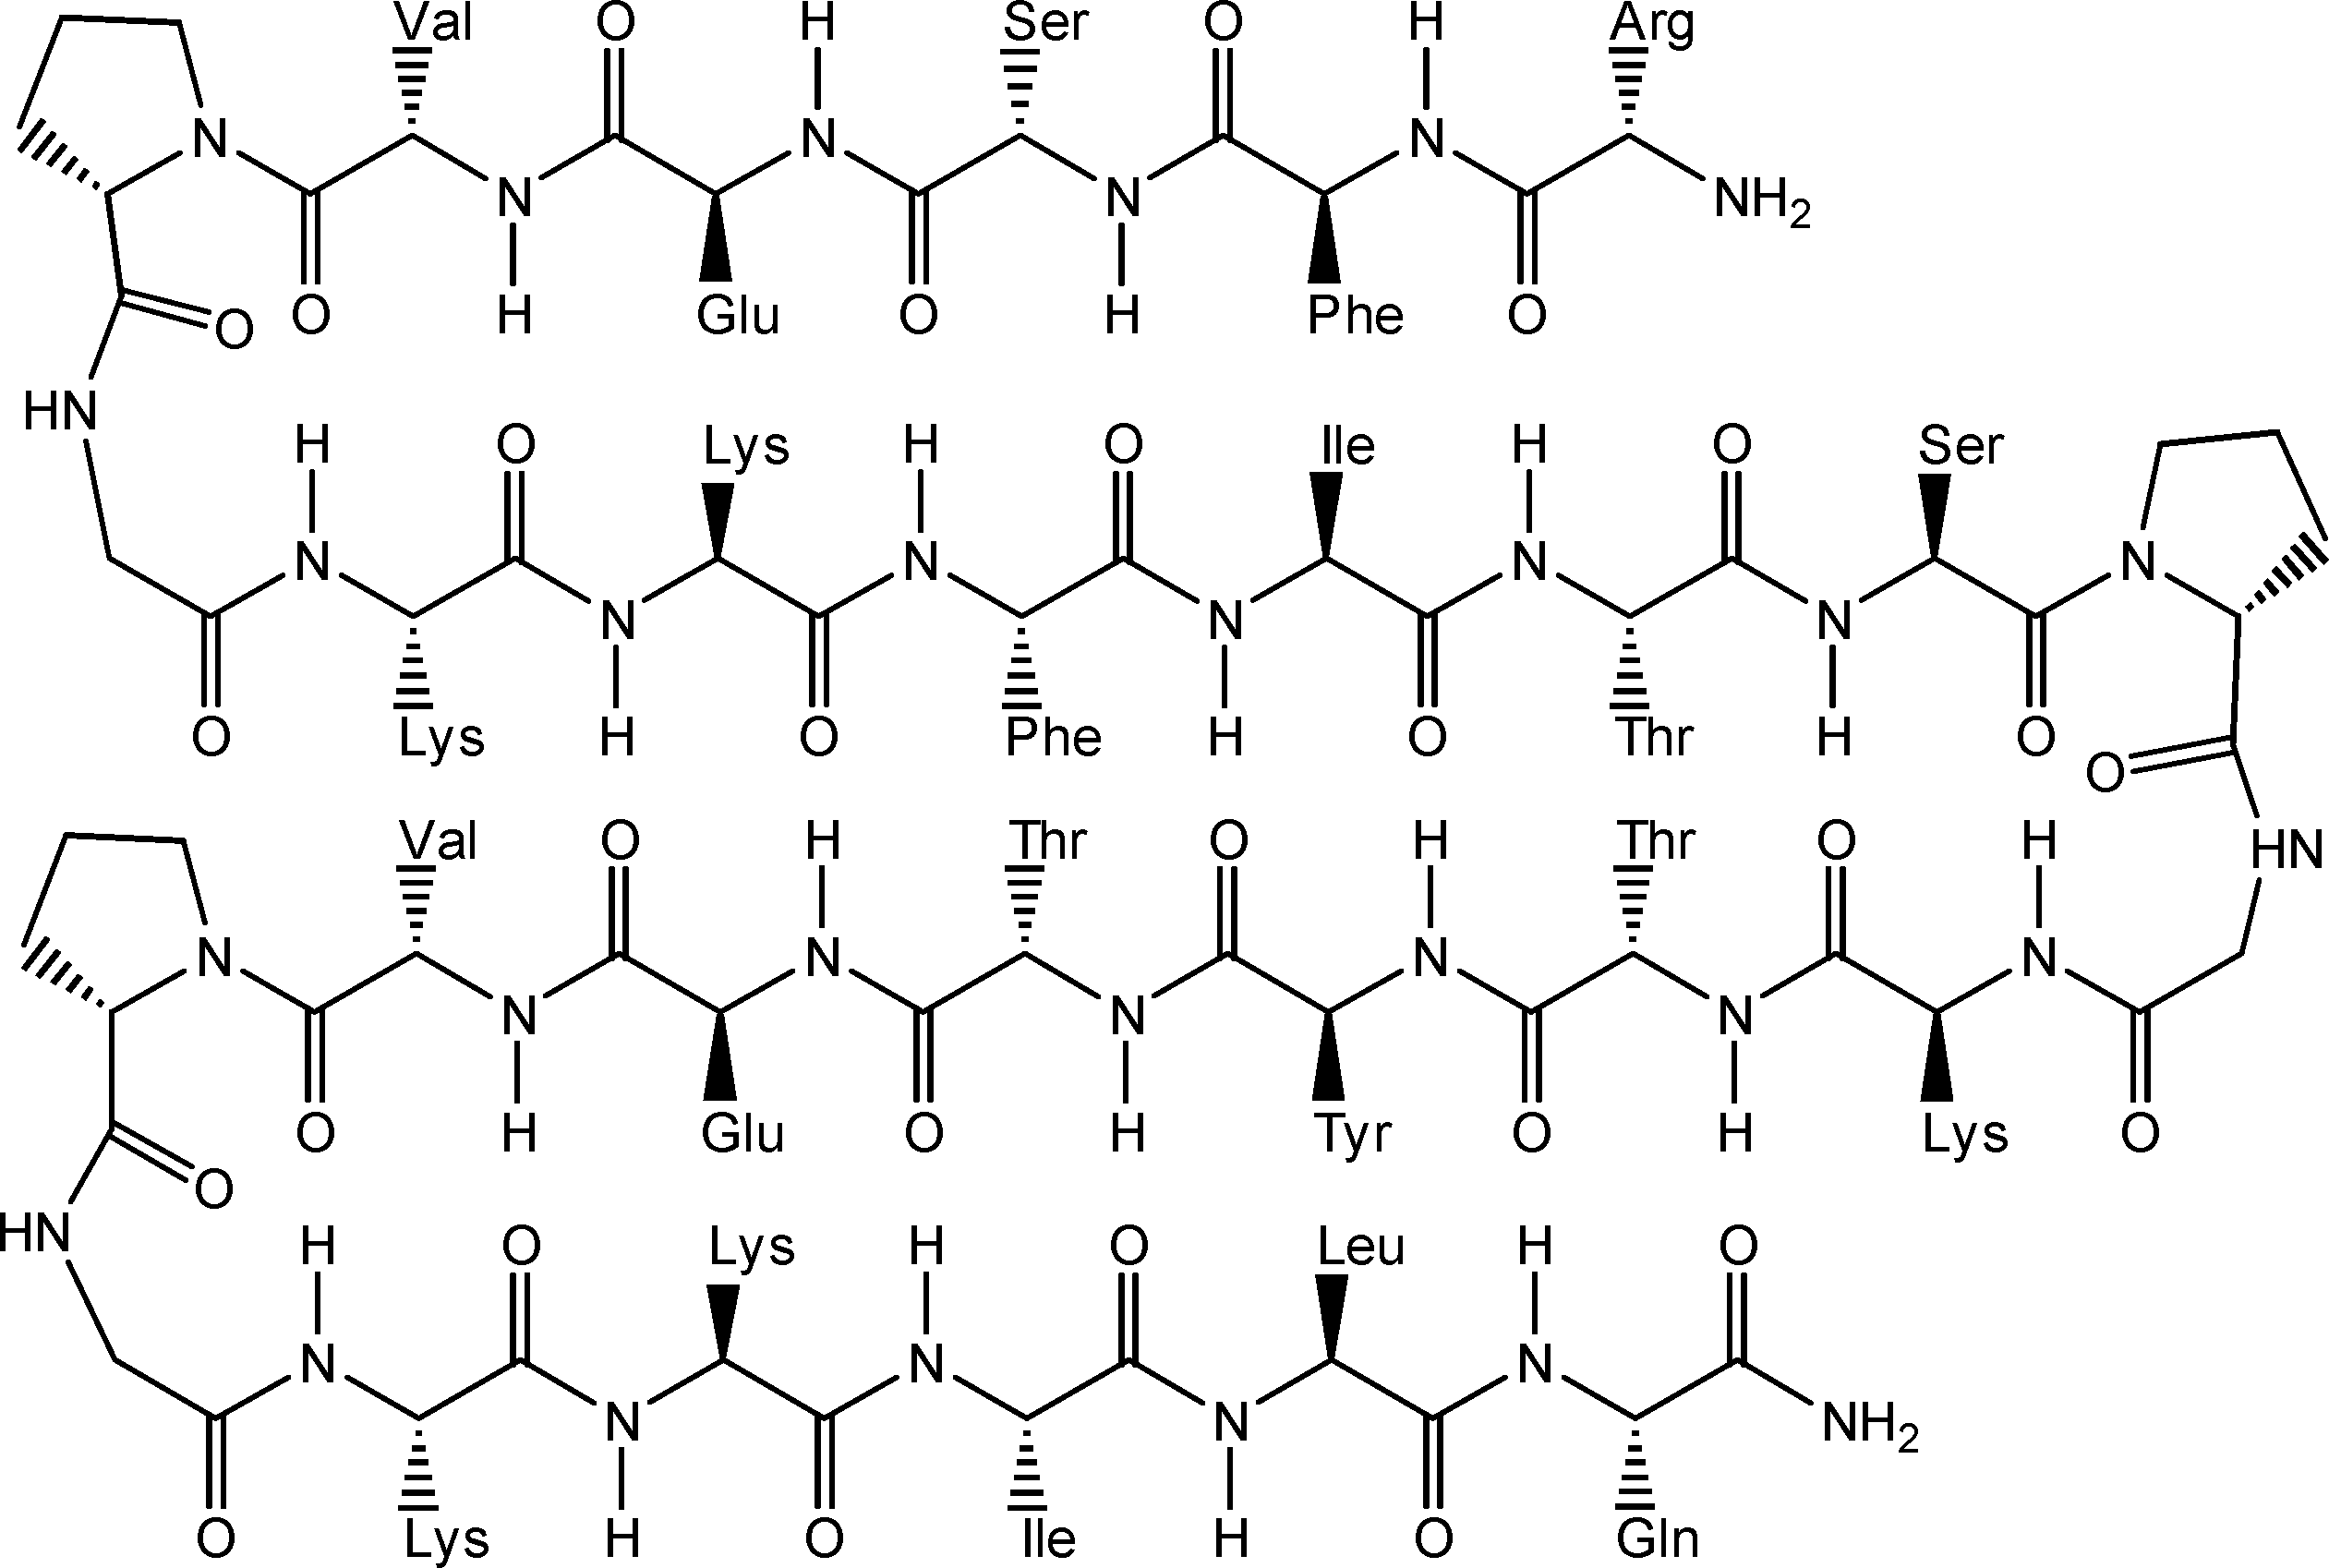
\includegraphics[width=\figurewidthSINGLE]{WL_crowding_paper/PIC_28_residue_seq_chem_sch.png}}
\caption{Native state of the peptide $^D$P$^D$P$^D$P represented schematically. The Pro-Gly amino acid residues at each end are combined to a single bead to allow for the proper turn structure on the fcc lattice. Image used with permission from Gai.\cite{xu_probing_2008}}
\end{figure}

\begin{figure}[ht]
 \subfloat[][Chemical Representation]{\label{fig:trpzip_residue_seq_chem_sch}
 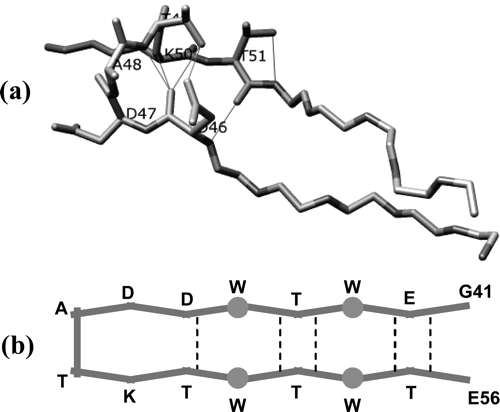
\includegraphics[width=\figurewidthSINGLE]{WL_crowding_paper/trpzipm1_du_pic.png}}
\caption{Native state of the trpzip-m1 peptide represented schematically. 
This image was generated from the NMR structure of trpzip4 (PDB code 1LE3, structure 1). The dashed lines represent the hydrogen bonds. Image used with permission from Gai.\cite{du_understanding_2006}}
\end{figure}

We use the WL method to calculate the conformations of the positional $\Omega_1 (\mathbf{c})$ and orientational $\Omega_2 (\sigma, \KP; \CHIX(\mathbf{c}))$ density of states. The model is calibrated by fitting $J_+$, $J_-$ and $h$ to the data of three experiments.\cite{xu_probing_2008, mukherjee_effect_2009,du_understanding_2006} We calculate the fraction of $\beta$-sheet contacts, observable from the experiments, by taking the expectation of $\avg{ \alpha \Theta(\alpha) }$. Here $\avg{\cdot}$ is the standard Boltzmann average, $\Theta$ the Heaviside step function and $\alpha(\mathbf{c})$ measures how close the protein is to its native state. Since the experimental data measures the fraction of $\beta$-sheet contacts (inferred from a circular dichroism measurement), we calibrated our model with physically similar observable, 
\begin{equation}
\alpha(\mathbf{c}) = (\KP-\KM)/ \KPMAX .
\end{equation}
This fraction of $\beta$-sheet contacts was used to calibrate the three free parameters. We note that without the non-native term $J_-$ in the Hamiltonian in Eq.\ (\ref{eq:Hamiltonian}) the fraction of sheet contacts would be, as usual $\avg{ \KP / \KPMAX }$.  In Figure \ref{fig:Exp_fits} we show the fits of the two proteins trpzip4-m1 and $^D$P$^D$P with the fitting parameters given in Table \ref{table:model_parameters}. The fits are quite good, encouraging us to make predictions about the system behavior as a function of crowding packing fraction. It is worth noting that the three and four stranded designed $\beta$-sheets had the best fits with $J_-=0$, implying that additional stabilization provided by the term was needed only to model trpzip4-m1. This may not be surprising when considering the larger melting points and the broad thermal transitions of the designed proteins versus that of the smaller $\beta$-hairpin peptide (listed in Table \ref{table:melting_points}).

\begin{table}
%\begin{ruledtabular}
\begin{tabular}{l|c|c|c}             
                & $h$   & $J_+$  & $J_-$  \\ \hline
Trpzip4-m1      & 9.396 & 6526.8 & 4691.6 \\
Three-stranded  & 5.103 & 2228.8 & 0.0    \\
Four-stranded   & 4.319 & 1751.3 & 0.0    \\
 \end{tabular}
 \caption{The fit parameters of the free energy (Eq. \ref{eq:free_energy}) to the model for each peptide. Here  $J_+$, $J_-$ are the strengths of the native and nonnative bonds and $h$ sets the energy scale of the dihedral angle term. }
  \label{table:model_parameters}
%\end{ruledtabular}
\end{table}

\begin{figure}[ht]
 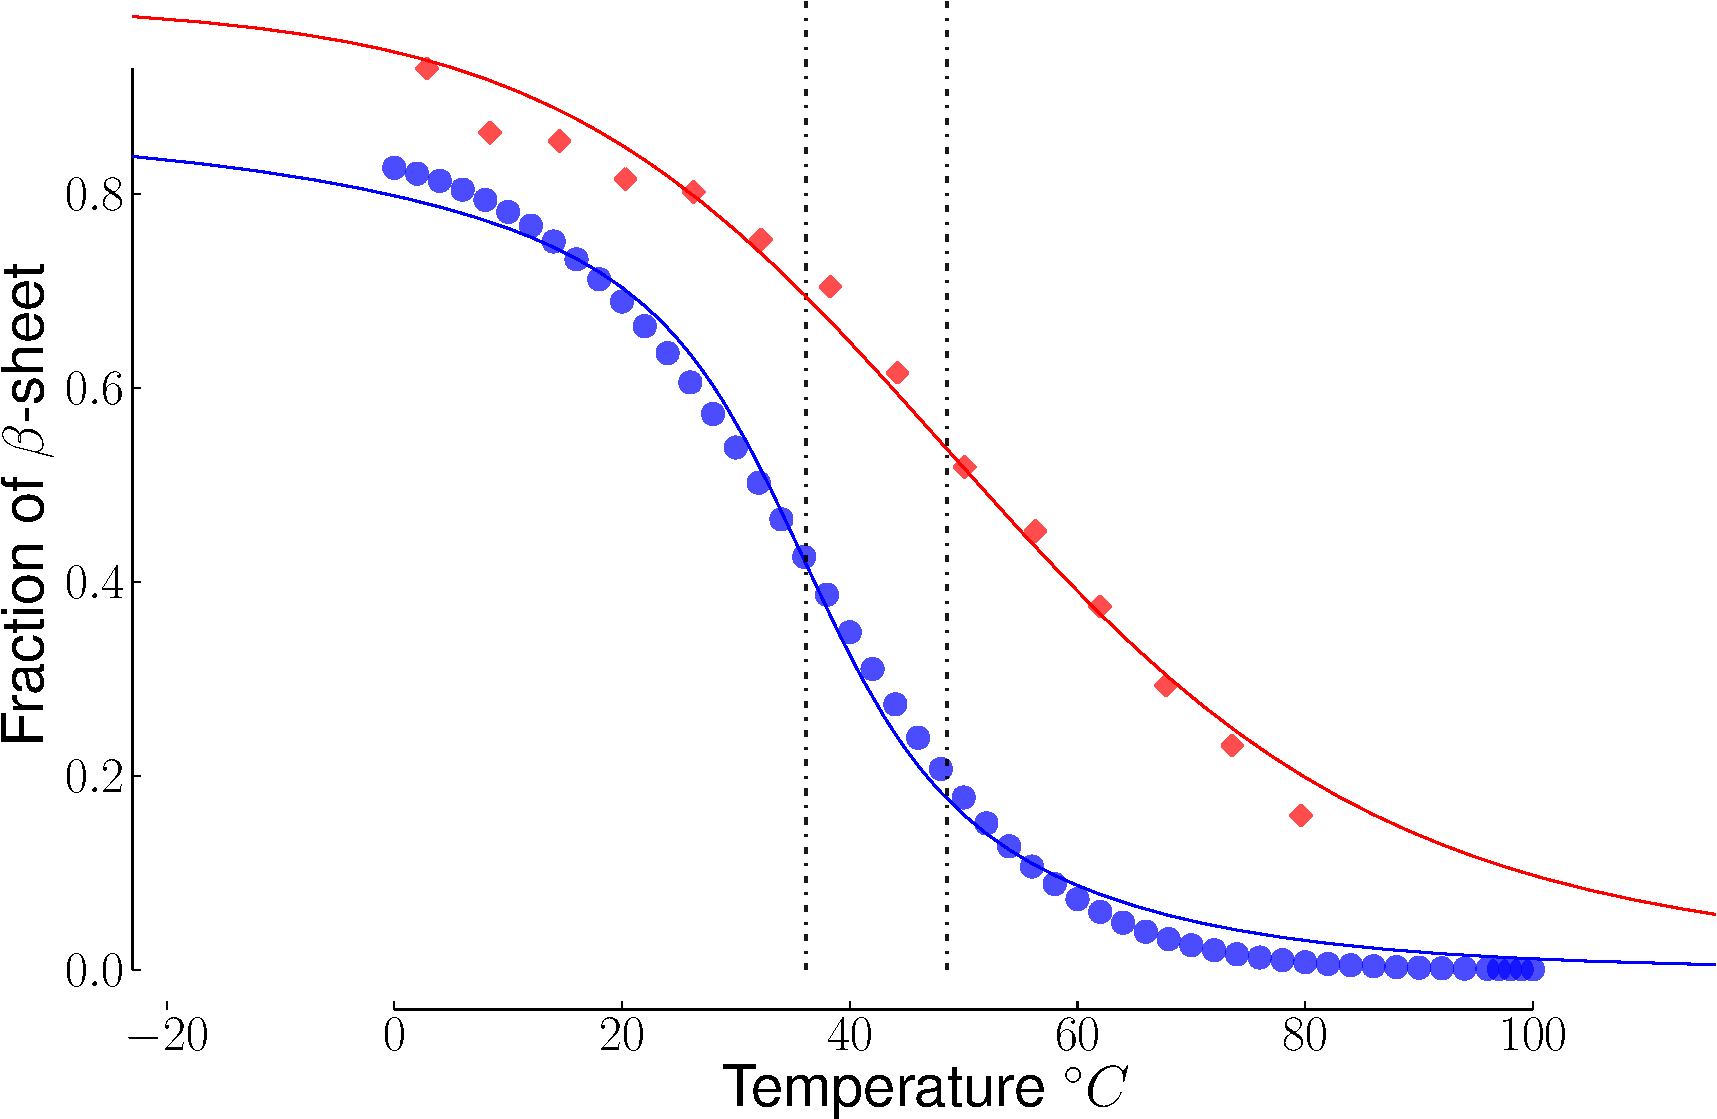
\includegraphics[width=\figurewidthSINGLE]{WL_crowding_paper/PLOT_all_experimental_fits-crop.pdf}
 \caption{Experimental data of fraction folded versus temperature for trpzip4-m1 (blue circles) and the three stranded $\beta$-sheet $^D$P$^D$P (red diamonds). Model fits are shown with dashed lines of the same color. The thin (black) vertical lines are shown to mark the critical temperatures at $36.1$ and $48.5$ $^\circ$C for three-stranded and trpzip4-m1 peptides respectively. The fit for the four stranded $\beta$-sheet $^D$P$^D$P$^D$P is similar to the three strand and is not shown for clarity.}
  \label{fig:Exp_fits}
\end{figure}

\subsection{Effects of Crowders}
In this section we use the model defined above to study the effects of crowders on peptide/protein structures and stability. For one of the peptides we have the experimental results on crowding effects to compare with. In the paper by Mukherjee \textit{et.\ al.\ }\cite{mukherjee_effect_2009} a significant change (approximately $12 ^\circ$C) in the melting point of trpzip4-m1 was observed  under crowded conditions. The crowder chosen for this experiment was Ficoll 70 (F70) at a concentration of $200$mg/ml. F70 is a compact, highly cross-linked branched co-polymer of sucrose and epichlorohydrin\cite{venturoli_ficoll_2005} with an average molecular weight of $70,000$. At $200$mg/ml, $300$mg/ml the packing fractions are approximately $\phi=0.13$ and $\phi=0.20$ respectively.\cite{lavrenko_separation_1987,dhar_structure_2010} We study the effects of crowders by considering the specific heat, $C_V(T) = \beta^2 \paren{ \avg{ E^2 } - \avg{E}^2}$ and note that in all cases, we observe only a single maxima. We identify this maxima as the melting temperature $T_C$ (alternatively, $\pfrac{C_V}{T} | _ {T_C} = 0$). 

Heat capacity as a function of temperature for trpzip4-m1 is shown in Figure \ref{fig:trpzip_CV_plot} while the melting points for all peptides listed in Table \ref{table:melting_points}.  As expected, trpzip4-m1 displays crowding enhanced stability with the change of critical temperature $\Delta T_c=[1.03, 1.65] ^\circ C$ at packing fractions $\phi=[0.13, 0.20]$ respectively. However, the three and four stranded $\beta$-sheets exhibit a slight decrease in their critical temperatures with $\phi$, indicating an entropically based \textit{instability} caused by the crowders. 
\begin{figure}[ht]
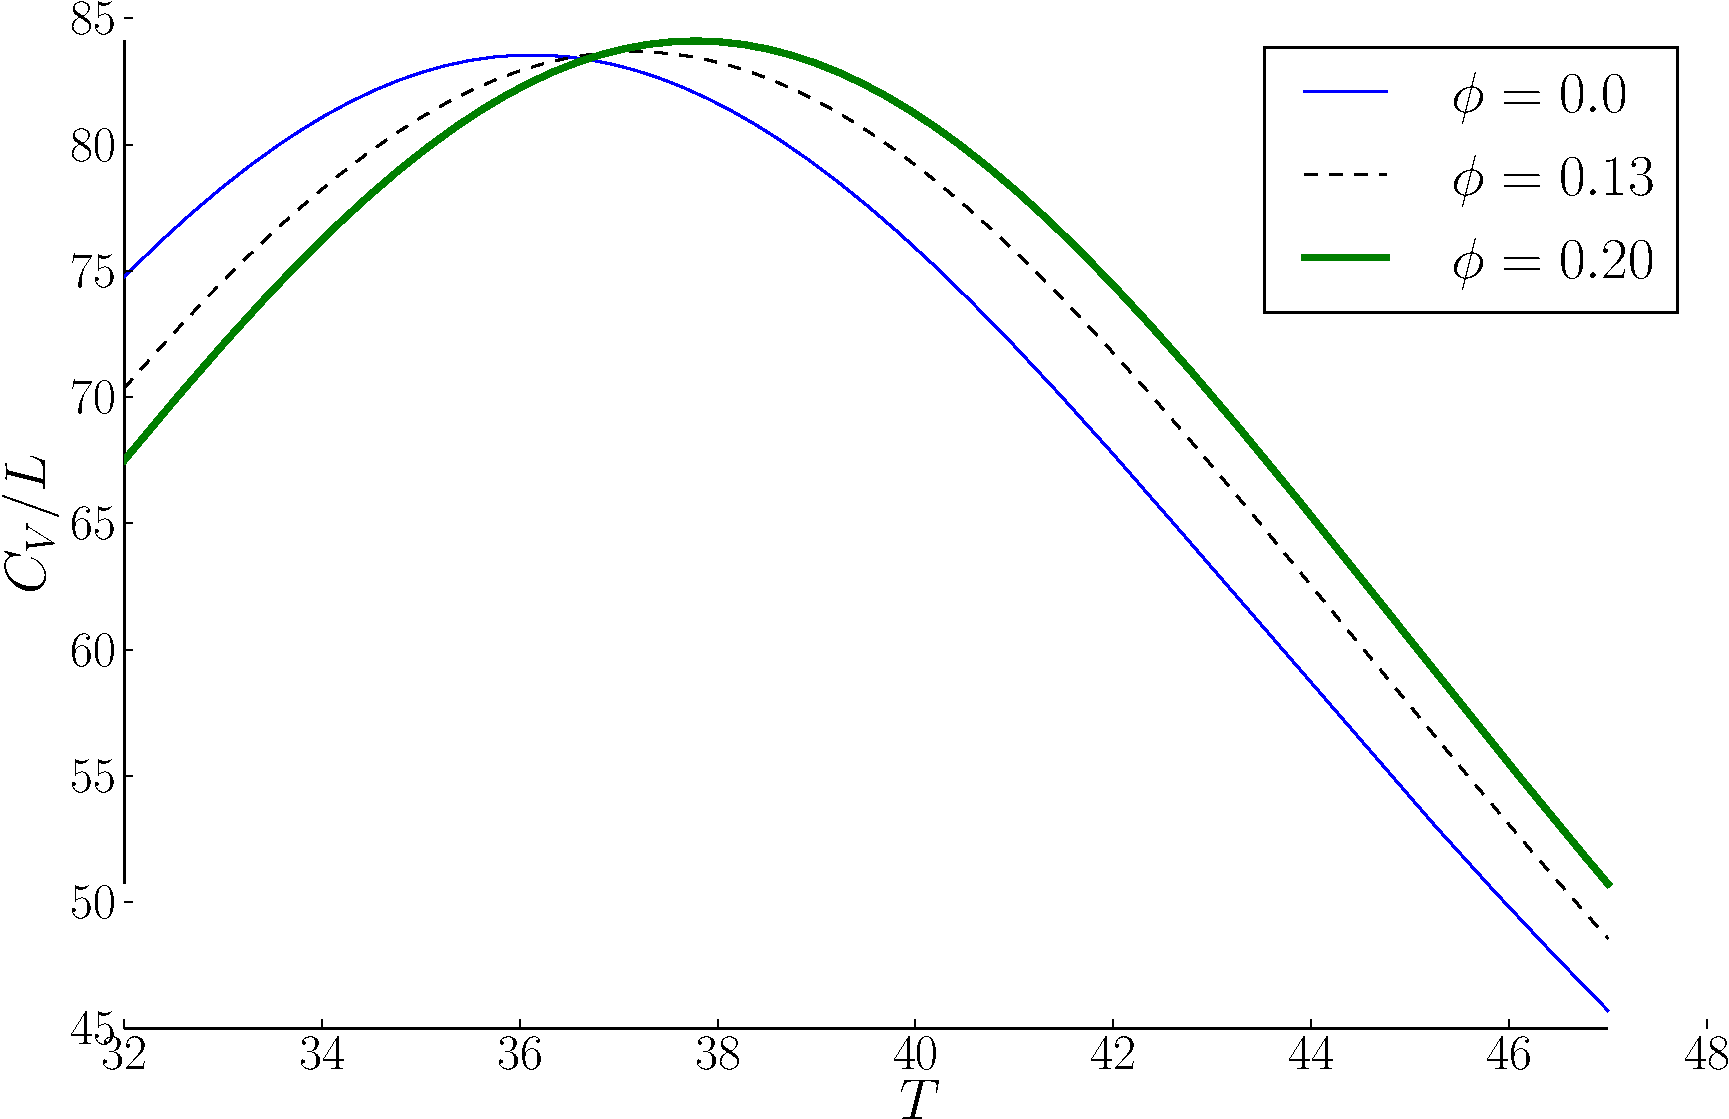
\includegraphics[width=\figurewidthSINGLE]{WL_crowding_paper/PLOT_trpzip_CV-crop.pdf}
\caption{Specific heat per residue count for the protein trpzip4-m1 in the presence of crowders.}
\label{fig:trpzip_CV_plot}
\end{figure}

%(309.12030531285251, 1) (310.14776783118413, 1) (310.77520920698208,    1.64
%(321.48930681998843, 1) (321.22525050654366, 1) (321.10529390266174,   -0.39
%(322.18103000528168, 1) (322.00889196768372, 1) (321.9355172255685,    -0.24 

\begin{table}
%\begin{ruledtabular}
\begin{tabular}{l|c|c|c|c|c}             
                          & Experimental    & $\phi=0$ & 0.13  & 0.20  \\ \hline
Trpzip4-m1                & $32.1 \pm 0.9$  & 36.12    & 37.15 & 37.76 \\
Three-stranded            & $52.6 \pm 0.4$  & 48.49    & 48.23 & 48.10 \\
Four-stranded             & $50.5 \pm 0.8$  & 49.18    & 49.01 & 48.94 \\
\end{tabular}
\caption{List of the experimental and model melting points (given in $^\circ C$) for each peptide. The experimental melting points are taken from \cite{xu_probing_2008, mukherjee_effect_2009, du_understanding_2006} in a dilute solution without crowders. The calculated melting points from the model are given at the listed values of the packing fraction. Not shown is the experimental value of trpzip4-m1 in the Ficoll 70 solution of $200$ mg/ml with $T_C=44.0 \pm 0.2$ $^\circ$C.}
\label{table:melting_points}
%\end{ruledtabular}
\end{table}

The native state for the three and four stranded $\beta$-sheets are highly aspherical. When considering the entropic effects of crowders, the system prefers compact conformations that minimize the excluded volume effect. As a consequence of this, the native state ceases to be the minimum free energy conformation at large enough $\phi$. Crowding-induced conformational change of the native state has been observed experimentally in a recent work by Dhar \textit{et.\ al.\ }\cite{dhar_structure_2010} who studied phosphoglycerate kinase (PGK) with the same crowders as our simulations (Ficoll 70). In this study, the conformational states were changed dramatically with crowders; an optimal non-zero packing fraction of crowders was found to increase the protein's activity. In our simulation, there was no shift to a new distinct native state at higher crowding concentrations. Rather, we observed a gradual shift towards more compact conformations at the expense of breaking energetically favored bonds, a general collapse of the $\beta$-sheet. As an example of the native conformation, which is enthalpically favored, versus an entropically favored one see Figure \ref{fig:sample_states}. Previous studies that showed crowding enhanced stability often dealt with globular wild-type proteins, whose natural environment required them to operate in crowded conditions. In contrast to the PGK study, the two larger peptides in our study were not wild-type, rather they were designed and studied because of the fact that they folded into beta-like conformations at realistic temperatures without aggregation. This suggests further experimentation on the designed peptides to determine if the destabilization of the native state against those of the unfolded and intermediate states under crowded conditions can be observed experimentally. 
\begin{figure}[ht]
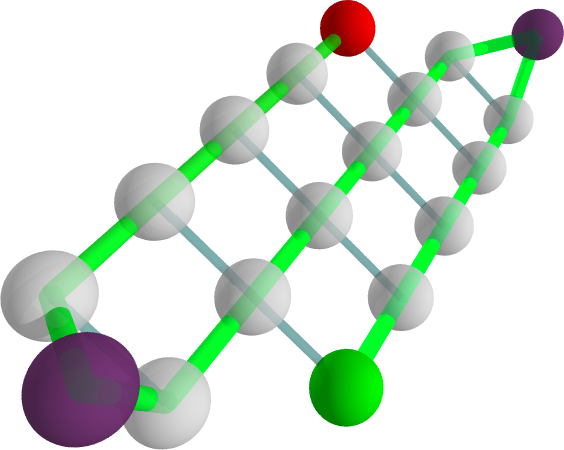
\includegraphics[width=5cm]{WL_crowding_paper/samplepic1.png} 
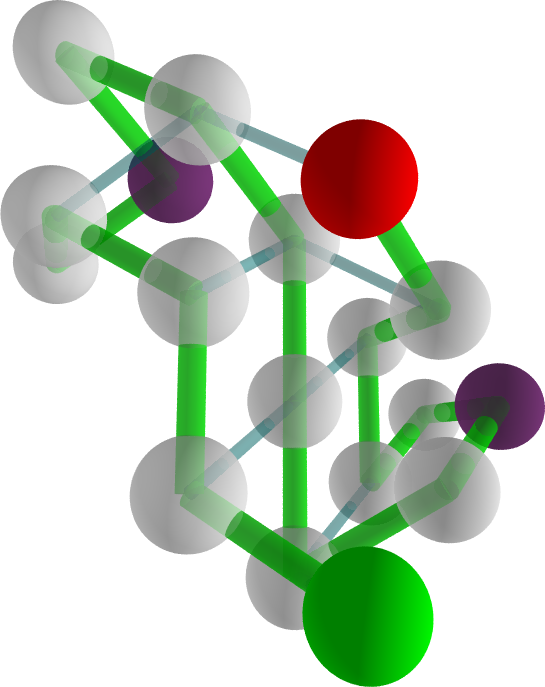
\includegraphics[width=5cm]{WL_crowding_paper/samplepic2.png}
\caption{Example of native state (top) and intermediate state (bottom) of the three-stranded peptide. The top state has ten bonds (shown as thin blue lines) while the bottom has eight bonds, making the native state favored energetically. However the ratio of activity coefficients $\ln \gamma_1 / \ln \gamma_2$ is $1.13$ at 200 mg/ml ($\phi = 0.13$) favors the eight bond structure due to the entropic crowding effects. The C and N terminus marked with red and green beads respectively and the combined Pro-Gly amino acid residues are purple beads.}
\label{fig:sample_states}
\end{figure}


In order to assess the effect on the conformational states we examine the Boltzmann averaged excess chemical potential from the native state as a function of temperature and $\phi$ 
\begin{equation}
\label{eq:d_mu}
\beta \avg{ \Delta \mu_{\text{ex}}(T) }  =  
\avg{ \ln{\gamma_i} - \ln{\gamma_N} }
.
\end{equation}
Figure \ref{fig:trpzip_chem_change_plot} of this free energy term for trpzip4-m1 illuminates several interesting structural features from an ensemble perspective. At large temperatures we see that this excess chemical potential approaches a constant, proportional to the change in the unfolded states due to the crowders. Conversely, at very low temperatures crowders have no effect on the only viable conformation, the native state. Near the folding transition temperature, the effect is large and non-linear.

\begin{figure}[ht]
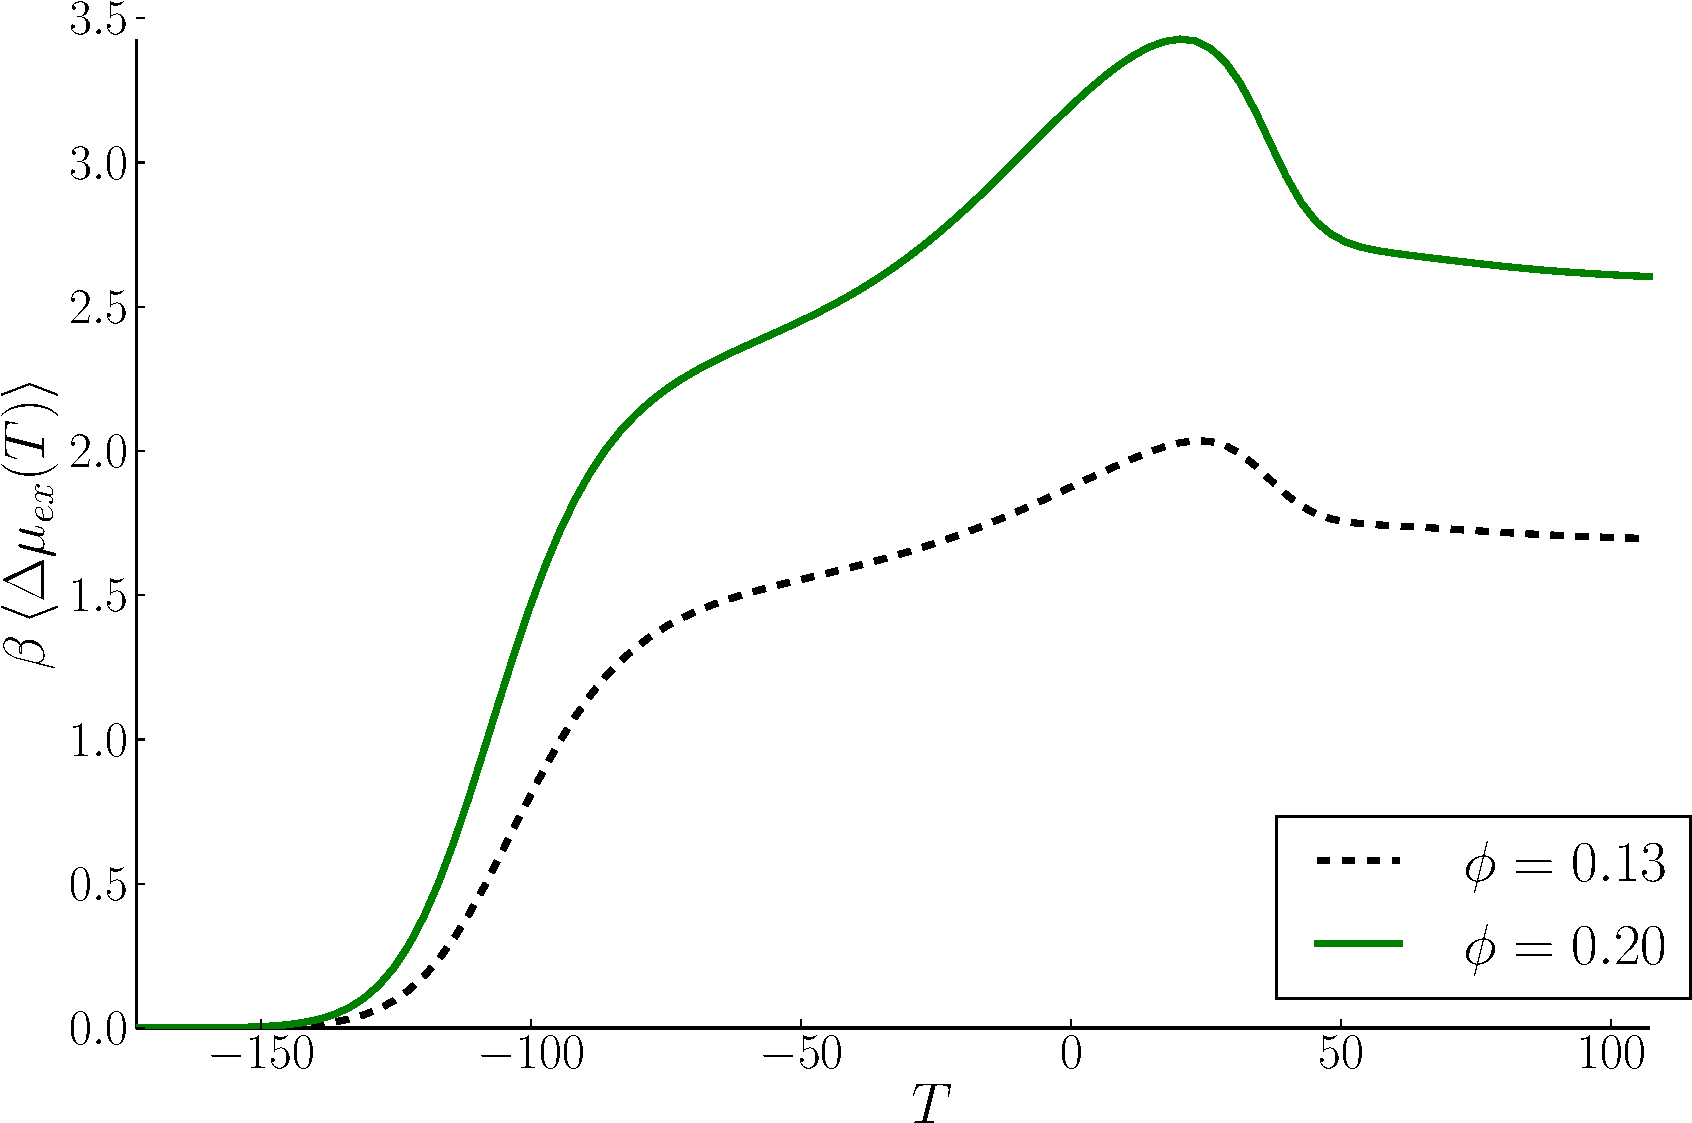
\includegraphics[width=\figurewidthSINGLE]{WL_crowding_paper/PLOT_trpzip_change_chem_pot-crop.pdf}
\caption{Excess chemical potential (defined in Eq. \ref{eq:d_mu}) for the protein trpzip4-m1 in the presence of crowders.}
\label{fig:trpzip_chem_change_plot}
\end{figure}



\section{Discussion \label{sec:conclusion}}
In this chapter we developed a coarse-graining model for proteins by combining the Ising-like state information of the dihedral angles of the modeled $\beta$-sheet structures with a fcc lattice model. The density of states has a favorable decoupling which enabled us to use the Wang-Landau method to determine the partition function accurately, giving excellent quantitative agreement with previous \textit{in vitro} experiments. Using our model and the predictions of SPT we found crowding-induced stability, in qualitative agreement with experiment for the smaller peptide, trpzip4-m1. The effect predicted by this model by showed a modest change of about $\approx 1^\circ$C, in contrast the the large change observed in the experiments of Mukherjee.\cite{mukherjee_effect_2009} We note however, that these coarse-grained models are approximations and selectively ignore various interactions. The study presented here is an entropic one. If the crowders have enthalpic interactions with the peptide, then these predicted effects will be incomplete. We attribute this underestimation to effects that cannot be explained by excluded volume effects alone.

We found that that the model predicted instability for the designed three- and four-stranded $\beta$-sheet peptides. This is consistent with the observation that their native state does not minimize excluded volume effects (it is disk-like rather then globular). This observation alone however, is not sufficient to predict of crowding based instability. Even if the native state is non-ideal, one has to consider the entire ensemble of states as a whole. This was possible using the Wang-Landau method which allowed us to accurately determine the density of states under the constraints of our model.  

The extension of the $\Go$-like contact map to a finite graph presented here is not limited to the $\beta$-sheet motif. This entropic model of conformational states can be extended to $\alpha$-helices or a mixture of secondary structures, as long as the contact graph structure can be decomposed into simple degenerate forms. 

\begin{comment}

\section{-= Working =-}

Given two conformations, $\mathbf{c}_1, \mathbf{c}_2$ and their respective density of states, we may want to determine when and under what conditions, the two states are equiproportional. That is, we would like to solve the free energy equation:
\begin{align}
\frac{ \mathcal{F}_1(\mathbf{c}_1)} {\mathcal{F}(\mathbf{c}_2) } &= 1 \\
\frac{ g_1 \exp( \beta( \sigma_1 h - k_1 J_+ + \Delta \mu(\mathbf{c}_1))  )  }
     {g_2 \exp( \beta( \sigma_2 h - k_2 J_+ + \Delta \mu(\mathbf{c}_2))  ) } &= 1 \nonumber 
\end{align}
This can be rearranged to give:
\begin{align}
\label{eq:criticalphiA}
\Delta \mu(\mathbf{c}_{12}))
&= \Delta \mu(\mathbf{c}_1)) - \Delta \mu(\mathbf{c}_1))  \\
&= \ln \paren{ \frac{g_1}{g_2} } + \beta h(\sigma_1-\sigma_2) - \beta J( k_1 - k_2) \nonumber
\end{align}

Using the values for $\Delta \mu(\mathbf{c}_12))$ from equation (\ref{eq:SPTcrowders}) we get:
\begin{align}
\label{eq:criticalphiB}
\Delta \mu(\mathbf{c}_{12}))
&= \frac{18\phi^3}{(1-\phi)^3} \paren{ \frac{R_1 - R_2}{2 r_c} } \\
&- \frac{18\phi^2(1+\phi)}{(1-\phi)^3} \paren{ \frac{R_1 ^2 - R_2 ^2}{4r_c^2} } \nonumber \\
&+ \frac{8\phi(1+\phi+\phi^2)}{(1-\phi)^3} \paren{ \frac{R_1 ^3 - R_2 ^3}{8 r_c ^3} } \nonumber
\end{align}

Combining equations (\ref{eq:criticalphiA}, and \ref{eq:criticalphiB}), gives us a polynomial in $\phi$ of third degree. If we hold the other parameters fixed (e\.g.\ $\beta, r_c$, \ldots) and let the native state correspond to $\mathbf{c}_2$, can numerically solve for this critical $\phi_c$. This $\phi_c$, if it exists and is physical,  corresponds to a switching point in the system. At this crowding concentration, the energetically favored native state is less likely to be found then a higher energy, but more compact conformation.
\end{comment}


  %CHAPTER: Generalized Aggregation Models
  \chapter{Aggregation Models}
\label{chap:potts_aggregation}

\section{Introduction and Motivation}
As we have seen in the previous chapters, the folding properties of a single protein are not only affected by the surrounding solution, but also the conformational state space available through confinement and excluded volume interactions. Up until this point we have considered the protein folding process as an independent event, including only an entropic solute interaction. In reality, there exist multiple biological events that feature enthalpic protein-protein interactions. Focusing on a subset, we apply our techniques to the study of aggregated species to model proteins that form composite structures which are larger and more complex than the sum of the individual elements.

Our study of aggregated species is primarily motivated by the devastating neurodegenerative disorder known as Alzheimer's disease. Alzheimer's is a progressive disorder that causes a deterioration of memory and cognitive function. The disease is the leading cause of dementia,\cite{querfurth_alzheimers_2010} effecting over thirty-five million people worldwide. The principal risk factor for contracting the disease is age, with the incidence doubling every five years after age 65. At 80 years old, one in six people have the disease.

Plaques of amyloid-$\beta$ (A$\beta$) fibrils are recognized as an important pathological feature in Alzheimer's disease. At normal physiological parameters, A$\beta$  is known to spontaneously self-aggregate into oligomers of two to six peptides. These in turn coalesce into larger forms. A$\beta$ can then grow into fibrils that form insoluble $\beta$-pleated sheets of amyloid plaques. However, it is the soluble oligomers and smaller amyloids that have been shown to be the most neurotoxic. This is evidenced by correlating the levels of the oligomerization with toxicity to synapses in brain-slice preparations.\cite{walsh_certain_2005} This is interesting, since the total amount of A$\beta$ plays less of a role than the intermediate growth phase.\cite{lue_soluble_1999} Structural information for the A$\beta$ peptide and its oligomers and fibril structure has been slow,\cite{kajava_beta-structures_2006} but recent results are beginning to emerge that detail these key features of the aggregation process.\cite{streltsov_crystal_2011} What is needed, is a general model that can incorporate these findings for A$\beta$ and other aggregation problems.  Aggregation studies of these proteins, and indeed all proteins in general, are essential to our understanding of the disease.

It is the aim of this chapter to develop and investigate several aggregation models with the tools introduced in this thesis. We begin with Section \ref{sec:first_order_aggregation}, where we develop a simplified first-order model. In it, we make several simplifying assumptions on the conformations and energies of the aggregated species. While the model is useful to develop intuition, we find that it is too restrictive and unable to provide a complete description about the aggregation process. To that end we generalize the first-order model in Section \ref{sec:potts_over_arbit_graphs} by reformulating the aggregation problem as the Potts model in an external field over an arbitrary graph. The main result of this chapter is the development and application of this solution as an operator expansion. With this method we are able to present new results on the Potts model problem. In Sections \ref{sec:one_d_ladder} and \ref{sec:two_d_ladder} we derive results for a one-dimensional `ladder' with thickness one and two respectively. Finally we present results in Section \ref{sec:edge_contraction_methods} for a wider class of problems with a subgraph recursion relation, albeit in the absence of external fields.

\section{First-order Aggregation}
\label{sec:first_order_aggregation}

Just as we coarse-grained the amino acid residues in Chapter \ref{chap:WL_crowding} to study the folding properties of a single protein, as we study the aggregation process we will make a suitable approximation for the larger length scale of aggregated species. In this section we will approximate an entire protein as one unit on a graph or lattice. Aggregation then, is a study of nearest neighbor contacts over this graph. 

Consider a simple interaction model over a square lattice with side length $L$ and $N=L^2$ sites with the Ising Hamiltonian
\begin{equation}
\HAM = -J \sum_{\avg{i j}} \sigma_i \sigma_j
\end{equation}
The lattice spacing is such that only a single particle can be occupied at any given site, hence $\sigma_i \in \{0,1\}$ corresponds to a lattice site being occupied or not. The interaction strength $J$, is related to the propensity for two proteins to be found next to each other. The summation extends over all nearest neighbors with a global restraint on the number of particles in the system $(m \leq N)$
\begin{equation}
\sum_i \sigma_i = m 
\end{equation}
Ultimately we want to set $N \rightarrow \infty$ corresponding to the thermodynamic limit. Thus we scale the interaction strength with the number if lattice sites as
\begin{equation}
J \propto \ln N
\label{eq:first_order_aggregation_scaling}
\end{equation}
%
The object of our study is a cluster or an oligomer, a collection of $m$ proteins that are connected through a path of nearest neighbors. For a given $m$ we partition the cluster configurations into combinations of clusters of different sizes and shapes. For example if $m=3$ we consider the partitions $[1,1,1], [1,2], [3]$ which correspond to 3 monomers, a monomer and a dimer, and a trimer, respectively. To the leading order in powers of $N$, the number of ways these configurations can be placed on the lattice are $N^3, N^2$ and $N$, respectively. We assume an individual $k$-mer is compact, it always its lowest energy state. On a 2D lattice this corresponds to an energy as a function of the cluster size $k$ 
\begin{equation}
 \HAM(k) = J \piecewisebrace{
 \begin{array}{lll}
   k + \lfloor k/2 -2 \rfloor & : & k > 1\\
   0                          & : & \text{otherwise}
 \end{array}
 }
\label{eq:piecewise_aggregation_eq_ham}
\end{equation}
%
where $\lfloor x \rfloor$ is the floor function. The partition function can then be written as
\begin{equation}
\Z = \sum_{p \in \text{partitions(m)}} N^ { \abs{p} }
\exp \paren{  - \beta { \sum _{k \in p} \HAM(k) } }
\end{equation}
This leads to several interesting properties. When $m$ is even it appears that there is a single first-order phase transition at $\beta_{1} = \frac{2m-2}{3m-4}$. When $m$ is odd and $m>3$ there are phase transitions at $\beta_{1}$ and $\beta_{2}=1$. These phase-transitions happen as the spontaneous collapse of the roots of a $m^{\text{\tiny th}}$ order polynomial equation. The type of phase-transition is logarithmic in $N$. 

\subsection{First-order pentamer model}
We illustrate the method with a worked example of the first-order theory with $m=5$. The set of partitions of $5$ particles (monomers to pentamers) is given by
\begin{equation}
\text{partitions}(5) = \{ [1,1,1,1,1],[1,1,1,2],[1,2,2],[1,1,3],[2,3],[1,4],[5] \}
\end{equation}
The energy of a single polymer in its configuration of maximally compact shape is given by Equation \ref{eq:piecewise_aggregation_eq_ham}: the monomers have energy proportional to 0, dimers 1, trimers 2, tetramers 4, 5-mers 5. Scaling the energy as in Equation 
\ref{eq:first_order_aggregation_scaling}, this gives the partition function as
\begin{equation}
\Z={N}^{5}+{N}^{4}{{\rm e}^{{ \beta}\,\ln  N }}+2\,{N}^{
3}{{\rm e}^{2\,{ \beta}\,\ln  N }}+{N}^{2}{{\rm e}^{3
\,{ \beta}\,\ln  N }}+{N}^{2}{{\rm e}^{4\,{ \beta}
\,\ln  N }}+N\,{{\rm e}^{5\,{ \beta}\,\ln  N
  }}
\label{eq:part_func_first_order_n_5}
\end{equation}
Using units where $k_B = 1$, the specific heat is $C_V = \beta^2 \pfrac{^2}{\beta ^2} \ln \Z$, we seek the discontinuities of $C_V$ as $N \rightarrow \infty$. Dropping the factor of $\beta^2$ this amounts to finding the discontinuities $C_V(\beta_C) = \infty$
\begin{equation}
\beta_C = \lim _{N \rightarrow \infty} \frac{1}{\ln N} \ln (\text{Roots}(f_5(x)) )
\end{equation}
with the polynomial $f_5(x)$ defined as
\begin{equation}
f_5(x) = n^5 + n^4 x + 2 n^3 x^2 + n^2 x^3  + n^2 x^4  + n x^5
\label{eqn:Worked_5_example_polynomial}
\end{equation}
%
\begin{figure}[ht]
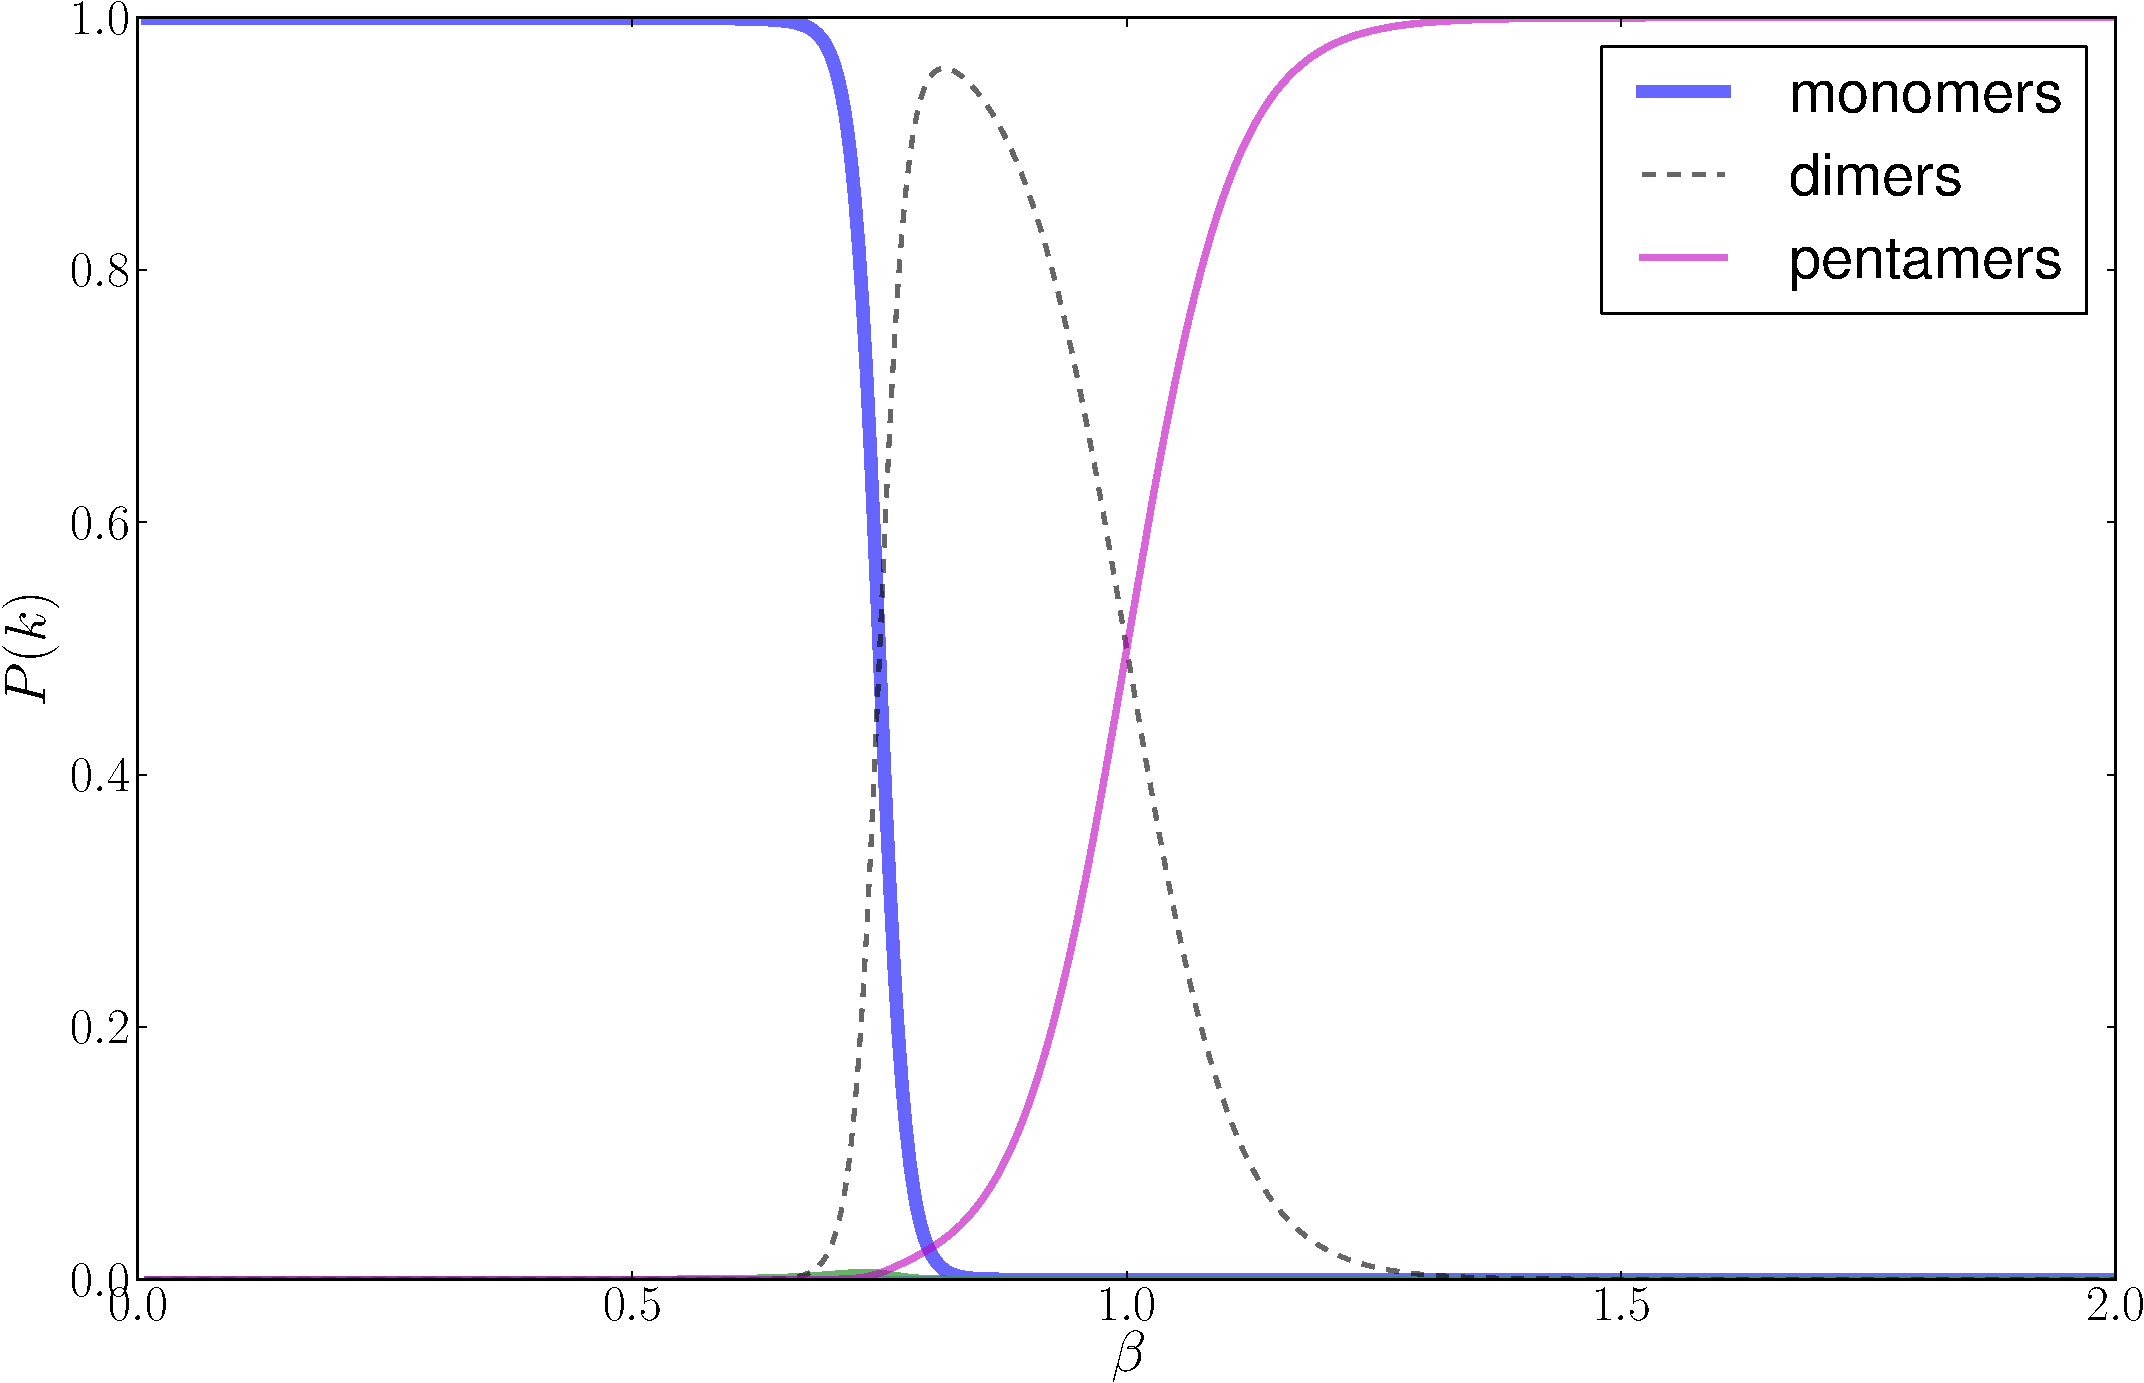
\includegraphics[width=.47 \textwidth]{pictures/aggregation_model/pictures/N=5_PZ.pdf}
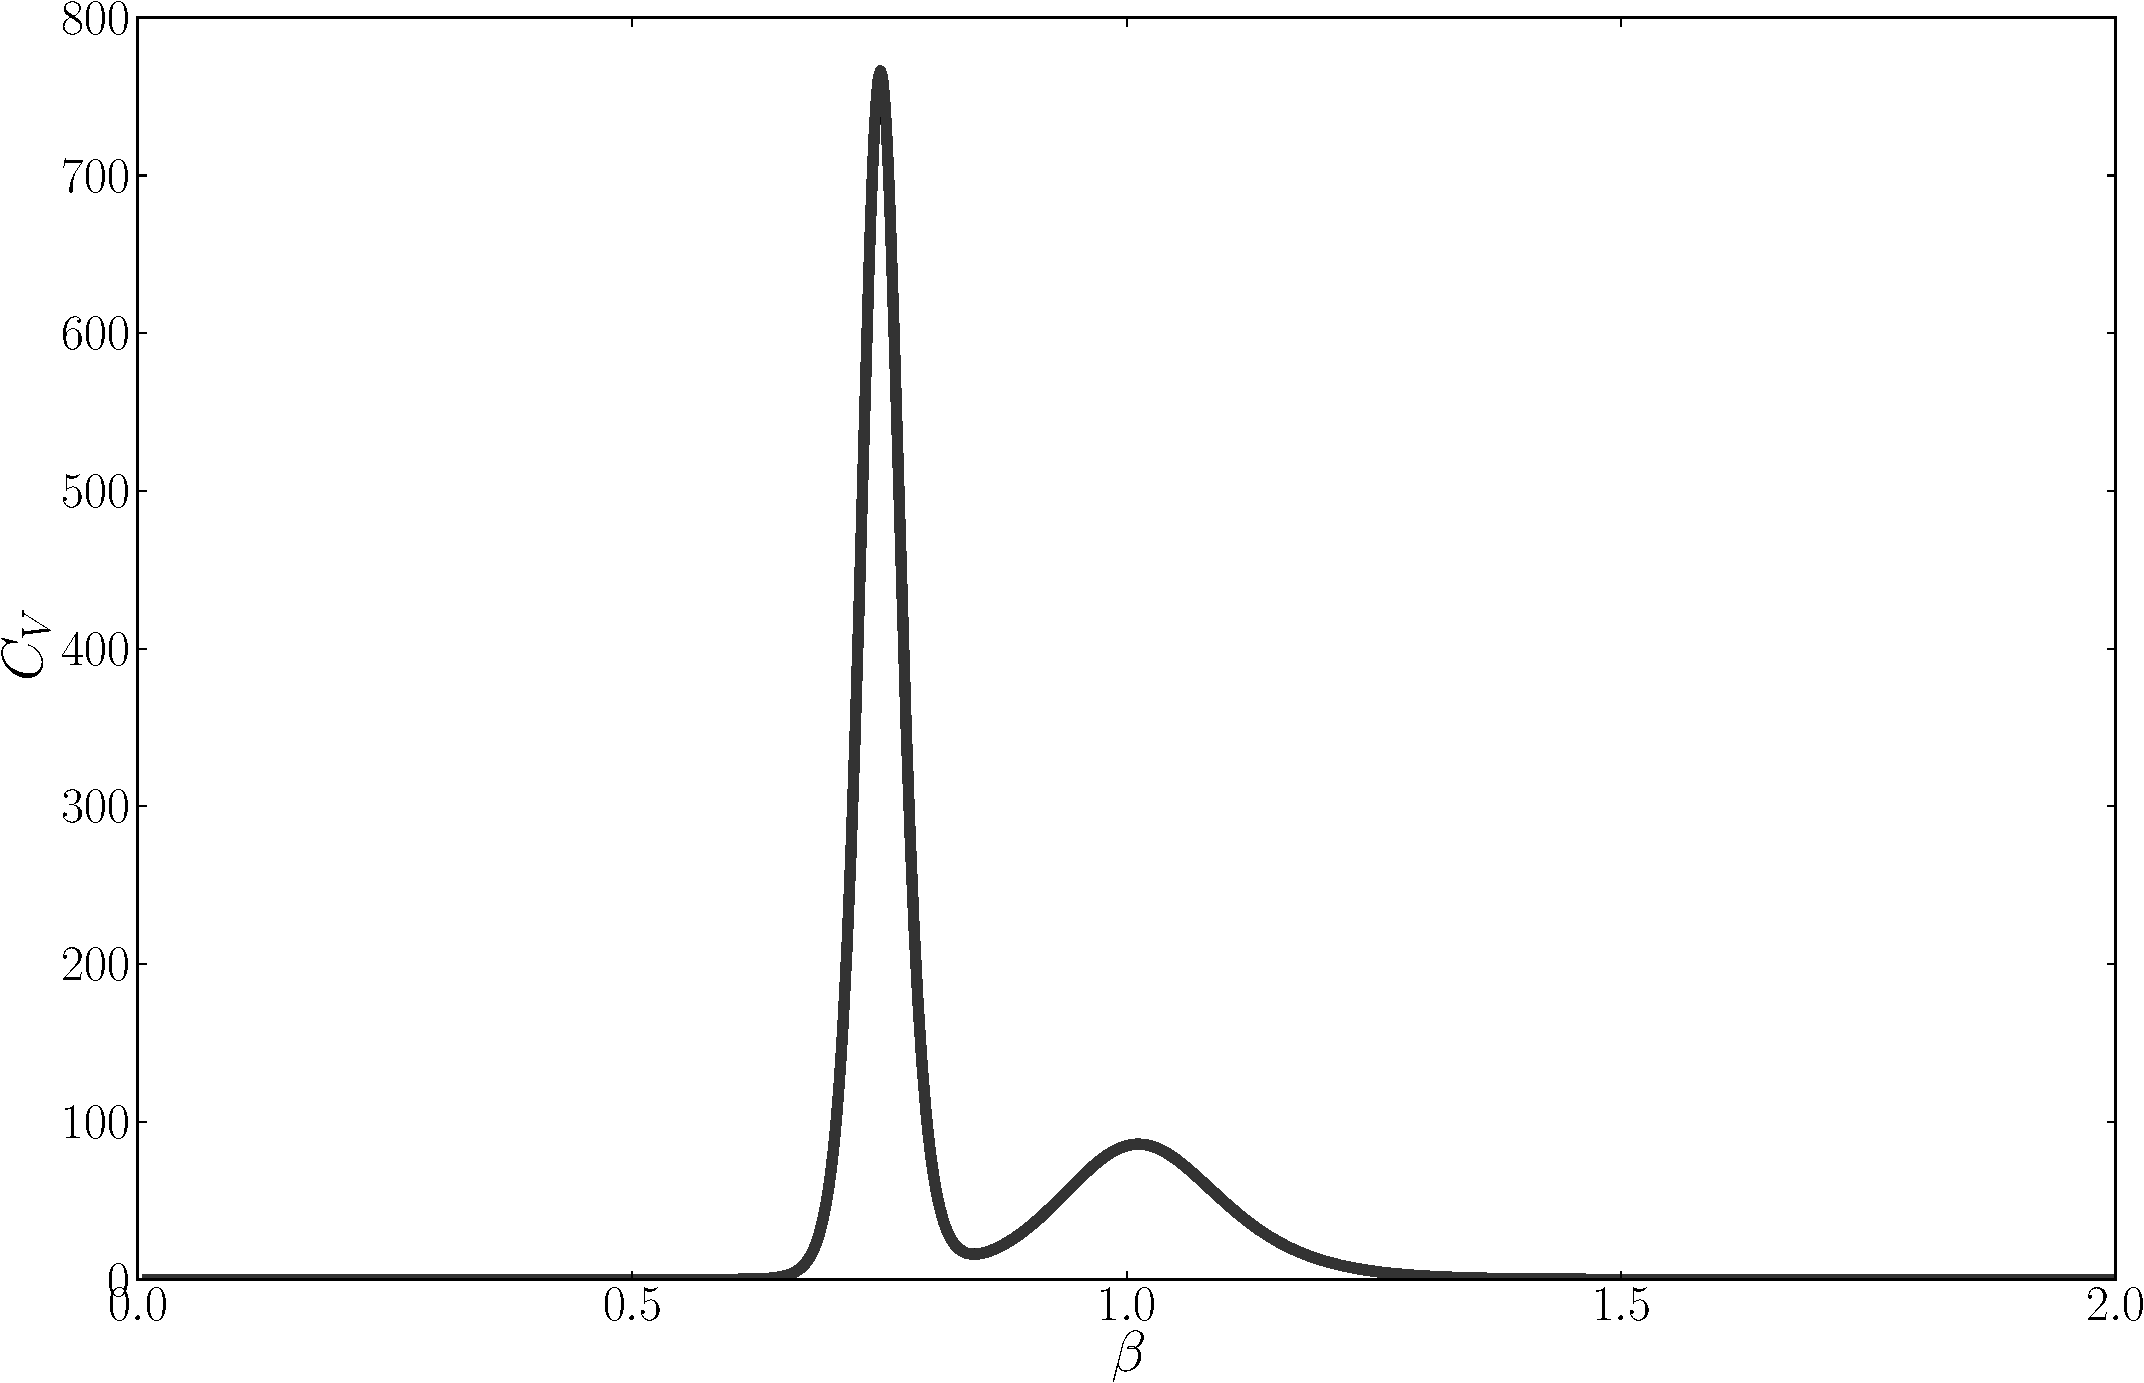
\includegraphics[width=.47 \textwidth]{pictures/aggregation_model/pictures/N=5_CV.pdf}
\caption{For the first-order aggregation model, the first graph shows the probability of each $k$-mer as a function of $\beta$ for the different conformations for the specific case of $m=5$. The second graph shows the specific heat as a function of $\beta$ for large $N$ ($N=10^{16}$). The large peak represents the first aggregation of monomers to dimers while the smaller peak signifies the collapse of the system to the lowest energy state of the pentamer. The trimers and tetramers have a low probability for all temperatures and are only visible near the transition temperature.}
\label{fig:Worked_5_example_picture}
\end{figure}
%
The coefficients to this polynomial come from the terms in the energy function. For this particular problem the solutions to equation \ref{eqn:Worked_5_example_polynomial} are
\begin{equation}
\beta_C = \braces{ 1, \frac{3}{4} }
\end{equation}
With a four-fold degeneracy on the $3/4$ root (see Figure \ref{fig:Worked_5_example_picture}). 

In the original work by Yang and Lee,\cite{lee_statistical_1952} they considered the grand partition function in terms of the fugacity. By extending the fugacity to the complex plane they used it to show that an Ising-like model will have complex roots on a unit circle. The expansion above is a continuation of this idea, except the parameter extended to the complex plane is $\beta$ and the zeros are known as Fisher zeros.\cite{fisher_1965_nature} In this case (as in many others), the zeros do not lie on a unit circle and produce intricate structures on the complex plane.

In Figure \ref{fig:zeros_part_func_first_order} we plot the phase angle of $\Z$ when temperature is continued onto the complex plane. The zeros of this function signify phase changes of the system. These zeros are visible on the complex plots by noting that around the poles the phase will change by a multiple of $2 \pi$. 

\begin{figure}[ht]
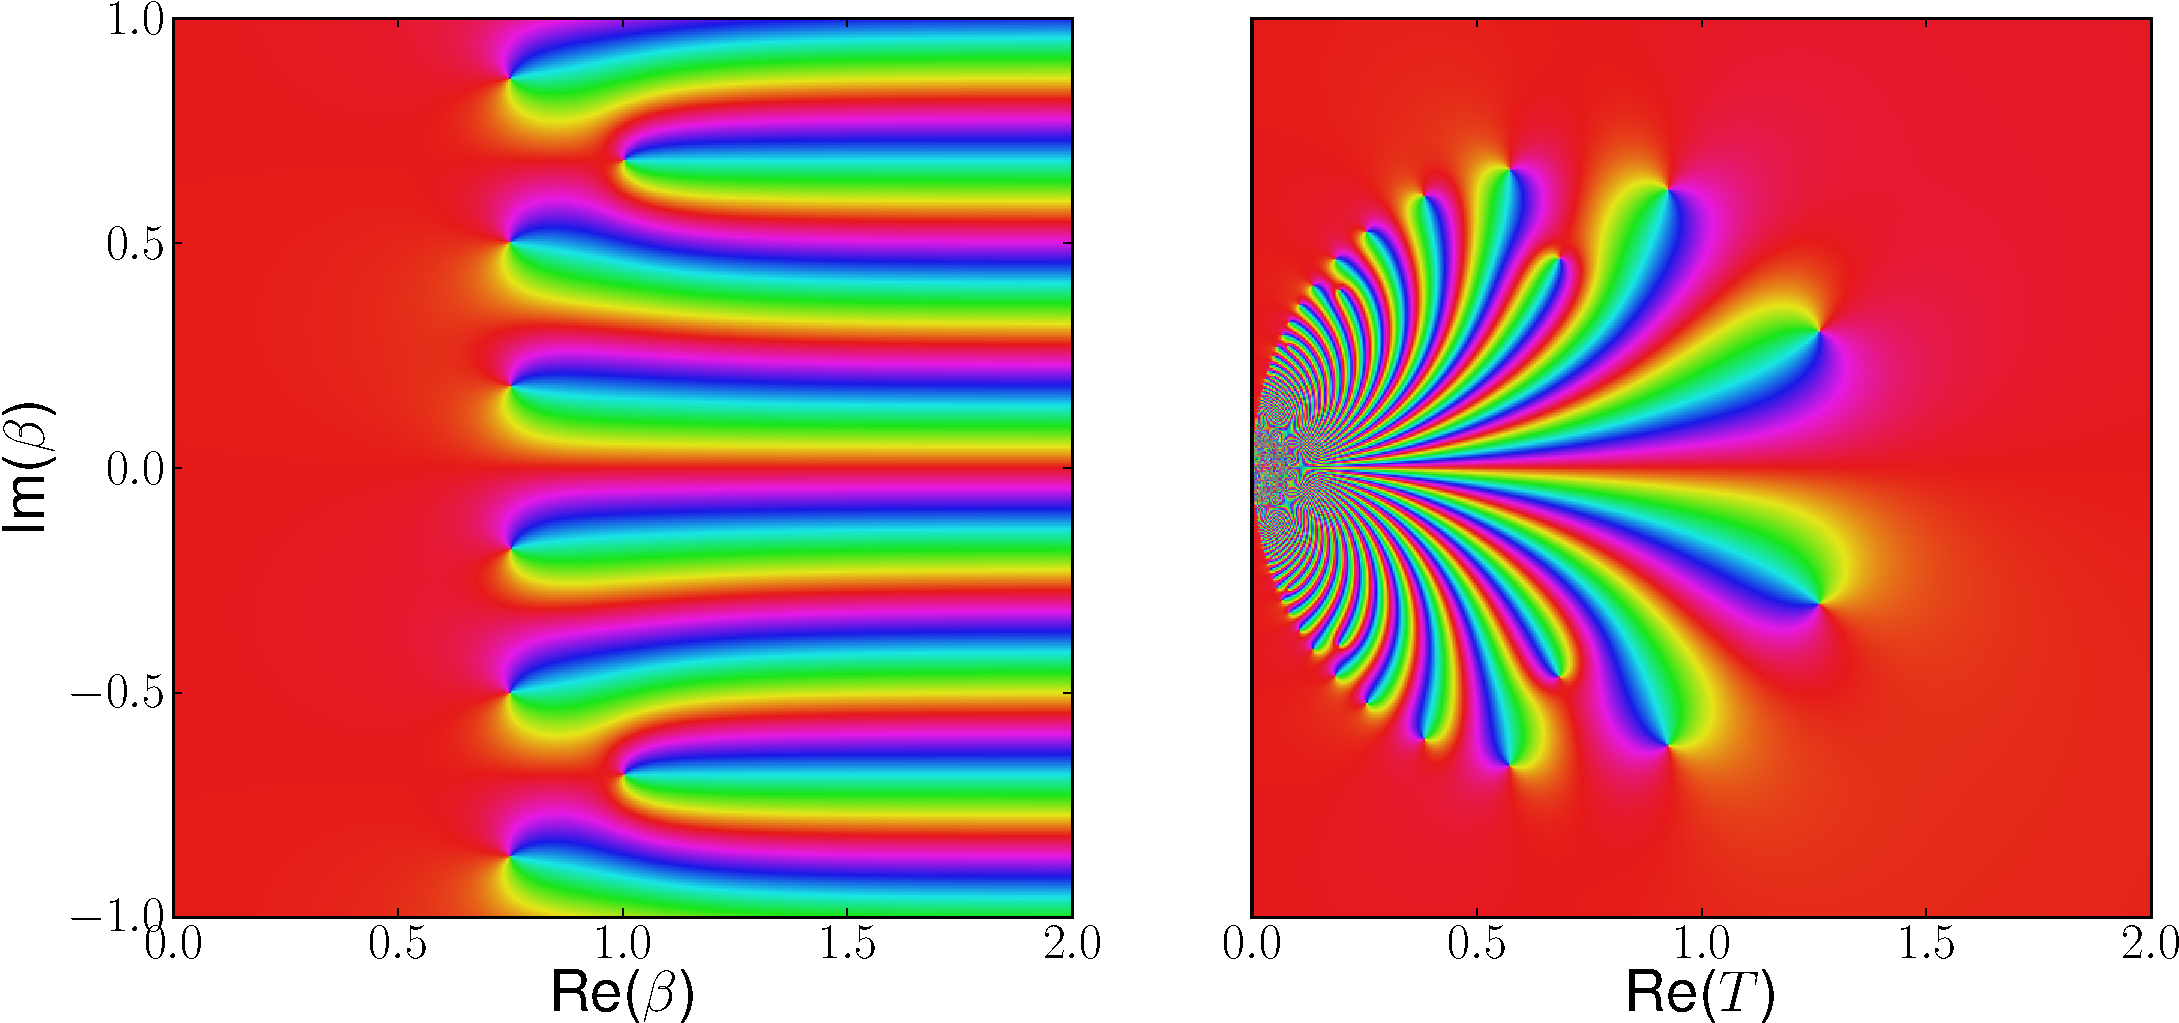
\includegraphics[width=\textwidth]{pictures/aggregation_model/pictures/f5_part_func_zeros.pdf}
\caption{Partition function of Equation \ref{eq:part_func_first_order_n_5} with $\beta$ analytically continued onto the complex plane. The colors of the graph mark the phase angle of the function, thus simple poles are marked by a complete change of color (due to Cauchy's theorem). The zeros at $\beta=1$ and $3/4$ can clearly be seen, but they have not yet collapsed onto the real plane due to finite $N$ (here $N=10^4$). Increasing $N$ alters the density of the zeros until they touch the real axis as $N$ goes to infinity.
}
\label{fig:zeros_part_func_first_order}
\end{figure}

We list the values of the function $f_n$ for several small $n$
{
\begin{align}
\label{eq:first_order_agg_series_list}
f_1(n) &= n 
\\ \notag
f_2(n) &= n^2+nx
\\ \notag
f_3(n) &= n^3+n^2x+nx^2
\\ \notag
f_4(n) &= n^4+xn^3+2x^2n^2+x^4n
\\ \notag
f_5(n) &= n^5+xn^4+2x^2n^3+x^3n^2+x^4n^2+x^5n
\\ \notag
f_6(n) &= n^6+xn^5+2x^2n^4+2x^3n^3+x^4n^3+x^4n^2+2x^5n^2+x^7n
\end{align}
}

\subsection{Drawbacks of the First-Order Model}

The model is interesting, but lacks the fidelity needed to model real aggregated proteins due to the approximations made. For one, the treatment of a protein as a single unit with uniform bond-strengths prevents the expression of any non-isotropic growth patterns. This is a severe limitation, as many fibril growths and aggregated species have a preferred growth direction after a minimal nucleation size. Along those lines, the assumption that the protein will aggregate only in the most compact and hence lowest energy conformation (via Equation \ref{eq:piecewise_aggregation_eq_ham}), may be valid for protein folding but is certainly invalid for many types of aggregated species. 

The scaling relation, Equation \ref{eq:first_order_aggregation_scaling}, was introduced in an ad-hoc manner to help retain a finite convergence of the critical temperatures. The motivating idea behind the approximations was to reduce the problem to the expression of a single polynomial whose properties could be studied analytically. Equation \ref{eq:first_order_agg_series_list} lists several values of the polynomial series $f_m$, but we did not find any interesting properties of the system. It is unknown if there is a deeper relation between this general aggregation model and this series.

Despite the shortcomings of this simple aggregation model, it provides an instructive tool to develop a more general method. To account for these approximations, we introduce more degrees of freedom into the system. We let the conformations take arbitrary shapes and potentials through a Potts model and define the boundary conditions by the graph the system is embedded in. We attempt to develop a solution to the Potts model over an arbitrary graph and discuss the possibilities this opens for modeling in the next section.


\section{Potts-Model over Arbitrary Graphs}
\label{sec:potts_over_arbit_graphs}

Computing the partition function $\Z$ of a model with short-range interactions is a standard problem in statistical mechanics. Indeed, the Ising/Potts model has attracted attention from fields as diverse as condensed matter to biophysics to economics.\cite{wu_potts_1982} The prototypical example is the Potts model, defined over a graph $G$ with $N$ vertices, edge set $\mathcal{E}$, and vertex set $\vec \sigma$.
%
\begin{equation}
\vec \sigma = \brackets{ \sigma_1, \sigma_2, \ldots, \sigma_N }
\end{equation}
%
Each vertex $\sigma_i \in \vec \sigma$ has a `spin' property.%
\footnote{
We use the term spin to keep with the original terminology of the Ising model. In our case the spin is not related to the electronic states of an atom, but rather a marker of the internal conformation states of the protein.}
%
In contrast to the Ising model, each spin can point in $q$ different directions
%
\begin{equation*}
\sigma_i \in \braces{ 1,2,3, \ldots, q } 
\end{equation*}
%
The Hamiltonian for the Potts model on a simple graph can be defined as
\begin{equation}
\HAM = - J \sum_{ \avg{ij} }  \delta(\sigma_i, \sigma_j)
       - h \sum_{ \avg{i} }  \delta(\sigma_i, \alpha) 
\label{eq:potts_model_ham}
\end{equation}
%
where the first summation goes over all edges, while the second summation goes over each vertex. Here $\delta$ is the Dirac delta function, $J$ is the strength of the bond interaction and $h$ is the strength of the external field (which acts only on spins pointing in direction $\alpha$). The system is fully specified by the arrangement of the spin at each vertex. Let $\sigma' \in \vec \sigma$ denote a particular set of spin conformations from the set of all arrangements. The partition function for the system is a sum over all such possible spin arrangements
\begin{equation}
\Z = \sum_{\sigma ' \in \vec \sigma} e^ { -\beta \mathcal{H}(\sigma ')  }
\end{equation}
%
We can expand the expression by noting that
\begin{align}
\label{eq:expanded_partition_function}
\Z &= 
      \sum_{\sigma ' \in \vec \sigma} 
      e^{ \beta J \sum_{\avg{ij}}  \delta(\sigma_i ' , \sigma '_j) }  
      e^{ \beta h \sum_{\avg{i}}   \delta(\sigma_i ' , \alpha) }  \notag\\
	&= \sum_{\sigma ' \in \vec \sigma}  
	\prod_{\avg{ij}} \brackets{ 1 + v \delta(\sigma_i ' , \sigma_j ' ) }
	\prod_{\avg{i}}  \brackets{ 1 + u \delta(\sigma_i ' , \alpha) }
	\notag
\end{align}
%
With the understanding that $v = e^{\beta J} - 1$, and $u = e^{\beta h} -1$. This gives a polynomial in $u$ and $v$ that reduces down to several other well known polynomials such as the Tutte and chromatic polynomial.\cite{godlin_graph_2008}

By definition, the partition function is the weighted sum over all possible states. Quite often physical problems can be approximated by a discrete (or countably infinite) set of interactions. The graph representing the interactions needs not be regular, and finding the exact solution has many direct benefits. The subgraph expansion method presented here is somewhat abstract, thus it will be worthwhile to have a toy system to illustrate each step of the process. We will apply the methods to a the simple three vertex graph illustrated in Figure \ref{fig:three_node}.
\begin{figure}[ht]
\TIKZgraphABC
\caption{Simple three vertex graph used in Section \ref{sec:potts_over_arbit_graphs} to illustrate the subgraph decomposition.
}
\label{fig:three_node}
\end{figure}

We first consider the case where there is no external field, $u=1$. Expanding out the partition function (with $\sigma_{ij} \equiv \delta(\sigma_i, \sigma_j)$ and $\bar \sigma_{i} \equiv \delta(\sigma_i, \alpha)$) for our toy model gives
%
{ \allowdisplaybreaks
\begin{align}
\mathcal{Z}_\text{toy} &= 
     \sum_{\sigma ' \in \vec \sigma} (1 + v \sigma_{12})(1 + v \sigma_{23})  
\\ %\notag
     &= \sum_{\sigma ' \in \vec \sigma} 1 
         + v(\sigma_{12} + \sigma_{23}) + v^2 (\sigma_{12} \sigma_{23})
\label{eq:subgraph_expansion_three_node}
\end{align}
}
%
Observe in Figure \ref{fig:three_node_subgraphs} the four subgraphs of $A \subseteq G$. These four graphs correspond exactly to the four terms of the partition function of Eq. 
\ref{eq:subgraph_expansion_three_node}. Each subgraph divides the graph into a collection of clusters, disjoint pieces that are not connected. Each term in the expansion survives only if \textit{all} of the delta functions inclusive to that cluster survive. For the empty graph with no edges, there are clearly $q^3$ ways of choosing the spins so the term survives. For the vertices with one edge, or identically two clusters, there are only $q^2$ ways to choose the spins as the requirement of a cluster with one edge forces two spins to be the same. For the subgraph with all the edges there are only $q$ ways to arrange the spins as each vertex must have the same spin. Thus each subgraph has a multiplicity over the spin states of $q^{k(A)}$ where $k(A)$ is the number of clusters in the subgraph. 

\begin{figure}[tb]
	\TIKZgraphABC 	\hspace{1em}
	\TIKZgraphAB	\hspace{1em}
	\TIKZgraphBC	\hspace{1em}
	\TIKZgraphC		\hspace{1em}
	\caption{
	The four possible subgraphs of a graph with edge set $\mathcal{E}=\{(1,2),(2,3)\}$. The cluster counting functions (Eq. \ref{eq:cluster_counting_function}) associated with each subgraph from left to right are $\CHI{3}{2}$, $\CHI{2}{1}\CHI{1}{0}$, $\CHI{2}{1}\CHI{1}{0}$, $\CHI{1}{0}^3$.
	}
	\label{fig:three_node_subgraphs}
\end{figure}

Note in the expansion of $(1 + v \sigma_{ij})$, each time a $\sigma$ term is picked up, a $v$ term is as well and each $\sigma$ term corresponds to an edge in the subgraph. With $A \subseteq G$ representing a particular subgraph and $e(A)$ denoting the number of edges in a subgraph, the partition function can be written as a sum over all the subgraphs rather than the vertices and edges
\begin{equation}
\mathcal{Z} = \sum_{A \subseteq G} q^{k(A)} v^{e(A)}
\end{equation}
This is the expansion first discovered by Fortuin-Kasteleyn.\cite{kasteleyn_1969} When this equation is applied to our toy system we get
%
{ \allowdisplaybreaks
\begin{align}
\mathcal{Z}_\text{toy} 
&= 
\sum_{\sigma ' \in \vec \sigma} 1 + v(\sigma_{12} + \sigma_{23}) + v^2 (\sigma_{12} \sigma_{23})
\\ \notag &=
\sum_{\sigma ' \in \vec \sigma} \left (
1 \prod_{j=1}^q \prod_{j'=1}^q \prod_{j''=1}^q \delta(\sigma_1, j) \delta(\sigma_2, j') \delta(\sigma_3, j'') \right.
\\ \notag
&\hspace{2em} + 2 v \prod_{j=1}^q \prod_{j'=1}^q \delta(\sigma_1, j) \delta(\sigma_2, j) \delta(\sigma_3, j')  
\\ \notag 
&\hspace{2em} + \left. 
v^2 \prod_{j=1}^q \delta(\sigma_1, j) \delta(\sigma_2, j) \delta(\sigma_3, j)  \right )
\end{align}
}
%
when the delta terms are taken into account this gives
\begin{align}
\mathcal{Z}_\text{toy} = q^3 + 2 v q^2 + v^2 q
\end{align}

We can compute the partition function in the presence of an external field by a similar trick. Let us first consider the second subgraph in Figure \ref{fig:three_node_subgraphs}, the graph with only a single edge joining vertices $2$ and $3$. There are two clusters $k(A)=2$, the cluster with one edge and vertices $v_1, v_2$ and the singleton cluster with vertex $v_3$. We consider the expansion
\begin{align}
\prod_{i=1}^2 \brackets{ 1 + u \delta(\sigma_i ' , \alpha) } &= 
 \brackets{ (1+ u \bar \sigma_2)(1+ u \bar \sigma_3) }
\brackets{ (1+ u \bar \sigma_1) } \notag \\
 &= \brackets{ 1+ u(\bar \sigma_2 + \bar \sigma_3) + u^2 (\bar \sigma_2 \bar \sigma_3) }
\brackets{ (1+ u \bar \sigma_1) } \notag
\end{align}
For the first bracketed term to survive in a subgraph expansion, all spins must be pointing in the same direction (namely that of $\alpha$) which gives a degeneracy of $q$ for the subgraph cluster. If, say $\bar \sigma_2 \neq \alpha$ then the term reduces to 1. Let the set of clusters in subgraph $A$ be $C_A = \{c_1, c_2, \ldots, c_{k(A)}\}$ and the number of vertices in a cluster as $n(c)$, we can rewrite the expansion as a product of the clusters:
\begin{align}
\prod_{c\in C_A} ^ {k(A)} \brackets{ w^{n(c)} - 1 + q }
\end{align}
%
Using the simpler form with $w=e^h$. This gives us the expansion by Wu\cite{wu_duality_1976} for the Potts model with an external field acting over a single spin by summing over the subgraphs:
\begin{equation}
\Z = 
\sum_{A \subseteq G}
v ^ {e(A)}
\prod_{c\in C_A} ^ {k(A)} \brackets{ w^{n(c)} - 1 + q }
\end{equation}

\subsection{Generalization to arbitrary field}
It is quite simple to let a field act in multiple directions. Instead of having a single $\alpha$ with strength $h$, we let $\vec a = \{h_1, h_2, \cdots, h_q \}$ be the vector that denotes the strength of the field acting on each spin direction. Since the fields are independent of each other (\ie the contribution from $h_1$ is independent of $h_2$, etc.) the derivation is identical giving
\begin{equation}
\sum_{A \subseteq G}
v ^ {e(A)}
\prod_{c\in C_A} ^ {k(A)} \brackets{ q + \sum_{j=1}^q \brackets{ (u_j+1)^{n(c)} - 1 }}
\end{equation}
%
Letting $w_i = e^{h_i} = u_i + 1$:
\begin{align}
\label{eq:partition_function_arbitary_field}
\Z &= \sum_{A \subseteq G}
v ^ {e(A)}
\prod_{c\in C_A} ^ {k(A)} \brackets{ q + \sum_{j=1}^q w_j^{n(c)} - \sum_{j=1}^q 1 } \\
&= \sum_{A \subseteq G} 
v ^ {e(A)}
\prod_{c\in C_A} ^ {k(A)} \brackets{ \sum_{j=1}^q w_j^{n(c)} } \notag
\end{align}

As an explicit example, if $q=2$, $w_1 = e^{h}$, $w_2 = e^{-h}$, $w^{-1}_2 = w_1 = w$, we have the standard Ising model in a field. The energy level spacing between the parallel and anti-parallel spins is 1 rather then 2, but this can be fixed by scaling $J$.
\begin{align}
\Z_{\text{Ising}} = 
\sum_{A \subseteq G} 
v ^ {e(A)}
\prod_{c\in C_A} ^ {k(A)} \brackets{ w^{n(c)} + w^{-n(c)} }
\end{align}

\subsection{Generalization to specific bonded interaction}

Here we expand the first term when we consider that every interaction does not have the same strength. In this generalization of the Potts model we let the energy of a bonded pair be
\begin{equation}
E_{ij} = J_i \delta(\sigma_i, \sigma_j) = J_i \sigma_{ij} 
\end{equation}
Where $\vec J = \{J_1, J_2, \cdots, J_q\}$ is a vector of the interaction strengths between spins of the same alignment. Ignoring the field term for a moment (as the term is independent in this partition function), our new Hamiltonian is
\begin{equation}
\mathcal{H} = -\sum_{\avg{ij}}\sum_{k}^q J_k \sigma_{ij} \delta(i,k)
\end{equation}
The partition function, in a form analogous to those described in previous sections, is
\begin{equation} \Z = \sum_{\sigma ' \in \vec \sigma} 
\brackets{ 
\prod_k^q \prod_{\avg{ij}} \paren{ 1 + v_k \sigma '_{ij} \sigma '_{ik} }
}
\end{equation}
Where $v_i = e^{\beta J_i} - 1$. For a given cluster in each subgraph $A \subseteq G$, the spins must all be aligned for the term to be non-zero. Each cluster, therefore, contributes for each edge and for all $J_i$. Thus:
\begin{equation}
\Z = \sum_{A \subseteq G} \prod_{c\in C_A}^{k(A)} \sum_j^q v_j^{e(c)}
\end{equation}

\subsection{Full Subgraph Generalization}

A $q$-state Potts model, defined over a graph $G$ with specific bonded interactions defined by $\vec J$ and an external field term acting on each spin direction with strength $\vec a$ has a partition function expressed as the sum over its subgraphs. When considering the product over the subgraphs we note that each associated subgraph has to have all the spins aligned, thus terms like $v_1 w_2 = 0$ in a subgraph multiplication. This gives
\begin{align}
\Z &= 
\sum_{A \subseteq G} \prod_{c\in C_A}^{k(A)} 
\sum_j^q \paren{ w_j^{n(c)} v_j^{e(c)} } 
\end{align}
%
Since we are counting properties of the clusters, we define the cluster counting function to count a cluster with $n$ vertices and $e$ edges as
\begin{align}
\CHI{n}{e} 
&= \sum_j^q \paren{ w_j^{n} v_j^{e} } 
\label{eq:cluster_counting_function}
\end{align}
%
A particular subgraph is the product of its cluster counting functions, while the subgraph expansion is the sum of all such products. In Figure \ref{fig:three_node_subgraphs} we list these terms for each subgraph of our toy model as an example. The full expansion of the Potts model with external field can then be expressed as a multivariate polynomial of the cluster counting functions
\begin{align}
\Z &= 
\sum_{A \subseteq G} \prod_{c\in C_A}^{k(A)} 
\CHI{n(c),}{e(c)} 
\end{align}

\section{Operator approach}
\label{sec:operator_approach}
%
Given a graph with $N$ vertices labeled $v_1, v_2, \ldots, v_N$, it will be useful to refer to a subset of these vertices. Let the $i^{th}$ subset be denoted $p_i=\{v_{i_1}, v_{i_2}, \ldots \}$. We associate with this subset two additional pieces of information and call it a subgraph partition, or simply a partition for short. These pieces of information are running tally of the edges and vertices as the operators process the vertices. These counts, $e_i$ and $n_i$, are not representative of current state of the partition, rather they represent placeholders for a counting algorithm.

We denote the $i^{th}$ partition by $P_i \equiv \pblock{p_i}{e_i}{n_i}$. For brevity in notation we omit the indices $\pblock{b_i}{0}{0} = \pblock{b_i}{}{}$ if the block has a zero count $e_i=n_i=0$. A basis state is specified by a collection of these partitions. Given a state $\ket{\psi}$ with $k$ partitions 
\begin{equation}
\ket{\psi} = \ket{\sum_{i=1}^k \pblock{p_i}{b_i}{n_i} } 
           = \ket{\sum_{i=1}^k P_i }
\end{equation}
%
For example, the 5 basis states for three vertices $1,2,3$ are
\begin{align*}
&\ket{ \pblock{1}{}{} \pblock{2}{}{} \pblock{3}{}{} } &
&\ket{ \pblock{12}{}{} \pblock{3}{}{} }  &
&\ket{ \pblock{13}{}{} \pblock{2}{}{} }  \\
&\ket{ \pblock{23}{}{} \pblock{1}{}{} }  &
&\ket{ \pblock{123}{}{} } 
\end{align*}
Each of these partitions represent a possible connection in the graph. A linear superposition of the basis states is simply called a state.

The idea is to write down a set of linear operators, that when applied to a specific graph, they reproduce all the subgraphs along with the prefactors needed for the partition function calculation. Our study was motivated by a recent paper by Bendini and Jacobsen\cite{bedini_tree-decomposed_2010} who gave an operator expansion to handle the Potts model without external fields. Their operators were 
\begin{itemize}
\item The join operator
\begin{align}
\B{J}_{ij} \ket{ \pblock{i}{}{}  \pblock{j}{}{} } &= \ket{\pblock{ij}{}{}} \\
\B{J}_{ij}^2            &= \B{J}_{ij}
\end{align}
\item The deletion operator
\begin{align}
\B{D}_{i} \ket{\pblock{i}{}{} \pblock{j}{}{} \ldots } &= q \ket{\pblock{j}{}{}\ldots} \\
\B{D}_{i} \ket{\pblock{ij}{}{} \ldots}  &=   \ket{\pblock{j}{}{} \ldots}
\end{align}
\end{itemize}
Note that the deletion operator applies the factor $q$ when the cluster is destroyed, thus it counts the number of clusters in the subgraph. This gives, as expected, a factor of $q^{k(A)}$. When a vertex is processed, for each edge $(i,j)$ connected to it they applied the operator $(\B{1} + v \B{J}_{ij})$ and finally the operator $\B{D}_i$ at the end of all the joins. 

\subsection{Operators with External Fields}
To compute $\Z$ with a field term we need to keep track of the number of vertices and edges in each cluster. Unfortunately the previous formulation by Bendini and Jacobsen destroys this information. We modify the state vectors so that each partition has two additional piece of information, $n(c)$ and $e(c)$. The new operators are defined to keep track of the pieces of information for each cluster. In all, we have four operators: vertex addition, removal, partition joins and global vertex renaming. The vertex renaming renaming operator is optional, but it facilitates the creation of composite operators that are useful for graphs with symmetry. The operators are
\begin{itemize}
\item Adding a new vertex: Adding a vertex to the state simply creates a new partition with a single vertex. Since this marks the beginning of a new cluster, the edge and vertex count is set to zero.
\begin{equation}
\B{A}_i \ket{\psi} = \ket{ \pblock{\{v_i\}}{0}{0} + \psi }
\label{eq:potts_operator_vertex_add}
\end{equation}
\item Joining two partitions: If $v_i \in p_1$ and $v_j \in p_2$ are the vertices to be joined, the partitions are combined by a set union and the vertices and edge counts are totaled together. An extra edge is added to reflect the new edge added to the partition.
\begin{equation}
\B{J}_{ij} \ket{\psi} = 
   \ket{ \pblock{p_1 \cup p_2}{e_1 + e_2 + 1}{n_1+n_2} + \psi - P_1 - P_2 }
\label{eq:potts_operator_vertex_join}
\end{equation}
\item Vertex removal: Removing a vertex can have two effects. Let $v_i \in p_1$ be the vertex to be removed. If the partition has more vertices than the one being removed $\abs{p_1}>1$, we remove the vertex and increment the vertex count by one.
\begin{equation}
\B{D}_{i} \ket{\psi} = 
\ket{ \pblock{p_1 / \braces{v_i}, }{e_1}{n_1+1} + \psi - P_1 } 
\label{eq:potts_operator_vertex_remove1}
\end{equation}
%
If the partition is a singleton (that is it contains only $v_i$), once this last vertex is removed the partition is complete. We can now count its contribution as a full cluster. The singleton partition $\pblock{p_1}{e_1}{n_1}$ picks up a factor of $\CHI{n_1 + 1}{e_1}$ with the $n_1 + 1$ term coming from the final vertex removal.
\begin{equation}
\B{D}_{i} \ket{\psi} = 
      \CHI{n_1 + 1,}{e_1} \ket{ \psi - P_1 } 
\label{eq:potts_operator_vertex_remove2}
\end{equation}
\item Vertex relabeling: If the vertices are labeled by 
$\mathcal{V} = \{ v_j,v_{j+1},v_{j+2},\ldots \}$, the operator $\B{T}_{i} \ket{\psi} $ shifts the labeling of all the vertices by a constant factor, $\mathcal{V} \rightarrow \mathcal{V}' = \{ v_{i+j},v_{i+j+1},v_{i+j+2}, \ldots \} $.
%
\begin{equation}
\B{T}_{i} \ket{\psi(v_1, v_2, v_3, \ldots)} =
               \ket{\psi(v_{1+i}, v_{2+i}, v_{3+i}, \ldots)}
\label{eq:potts_operator_vertex_relabel}
\end{equation}
\end{itemize}
An individual operator is commutative with others of its type, \ie 
$\B{J}_{ij}\B{J}_{mn} = \B{J}_{mn}\B{J}_{ij}$ but two different types of operators are not. This makes physical sense, one can not join a vertex until it is created.

\subsection{Vertex Processing}
%
With the operators defined, we now need a way to process the vertices of a graph. With the set of edges defined as $\mathcal{E}$ the most na\"{\i}ve approach would be
\begin{equation}
\sum_{v_i \in V} \B{D}_{i} 
\sum_{(v_i, v_j) \in \mathcal{E}} (\B{I} + \B{J}_{i, j})
\sum_{v_i \in V} \B{A}_i
\ket {\emptyset} 
\end{equation}
Where $\emptyset$ is the empty graph. This is however, horribly inefficient. If there are any common subgraphs, this process ignores any inherent symmetries. A more efficient method would remove vertices as soon as all their contributions were considered. This approach can be encapsulated with a composite operator $\B{L}$. Taking the vertices in lexicographic order we follow the following prescription at the ith step: add the target vertex and all vertices sharing an edge with the target vertex where $i<j$, delete the target vertex and repeat for all vertices
\begin{align}
\label{eq:vertex_linear_processing}
\B{L}_i &=
\B{D}_{i} 
\sum_{(v_i, v_j) \in E} (\B{I} + \B{J}_{i, j})
\brackets{ \sum_{(v_i, v_j) \in E, i<j} \B{A}_j }
\B{A}_i
\end{align}

An optimal method of vertex processing would use a tree-decomposition of a graph. In a tree-decomposition, the vertices are mapped onto a separate tree graph (a graph with no cycles).\cite{robertson_graph_1984} That is, the vertices of the tree graph $\braces{ u_1, u_2, \ldots}$ contain subsets of the vertices of the original graph $u_1 = \braces{v_{j_1}, v_{j_2}, \ldots}$. The vertices are mapped such that each vertex pair representing an edge on the original graph is contained within some vertex in the tree graph. Additionally, if vertex $v_1$ is contained in both $u_1$ and $u_2$ than each vertex along the unique path connecting $u_1$ and $u_2$ must also contain $v_1$. The tree vertex with the largest cardinality $\max(\abs{u_i})$ is known as the tree-width. While it is $\mathcal{NP}$-hard to determine the optimal tree-decomposition of a graph,\cite{arnborg_complexity_1987} once known many graph algorithms that are $\mathcal{NP}$-hard can be computed in polynomial time, bounded by the tree-width.\cite{arnborg_linear_1989}

Given a tree decomposition of the graph, the vertex processing outlined in Equation \ref{eq:vertex_linear_processing} could be greatly improved. To do so however, would require a new operator, one that fuses the partition when joined together on the tree-decomposition. In this chapter we only work with the lexicographic order of processing. For our purposes it straightforward to apply the simpler lexicographic order to the larger ladder graphs considered in the later sections.

\subsubsection{Worked example of Figure \ref{fig:three_node}}
We now work through our toy graph as an example of the operators with a standard path decomposition. The full process is
\begin{align*}
\ket{\psi_3} &= \B{D}_3
                \B{D}_2 (\B{1} + \B{J}_{23})
                \B{A}_3
                \B{D}_1 (\B{1} + \B{J}_{12})
                \B{A}_2 \B{A}_1
                \ket{\emptyset}
\end{align*}
The operators applied at each step:
\begin{align*}
\B{A}_2 \B{A}_1 \ket{\emptyset} &= 
\ket{ \pblock{1}{}{} \pblock{2}{}{} } = \ket{\psi_0} \\
%
\B{D}_1(\B{1} + \B{J}_{12}) \ket{\psi_0} &= 
\B{D}_1 \paren{ 
  \ket{\pblock{1}{}{} \pblock{2}{}{}} + 
  \ket{\pblock{1 2}{1}{}}  }
  = \CHI{1}{0} \ket{ \pblock{2}{}{} } 
     + \ket{\pblock{2}{1}{1}} = \ket{\psi_1} \\
  \B{D}_2 (\B{1} + \B{J}_{23}) \B{A}_3 \ket{\psi_1} &= 
  \B{D}_2 \paren{ \CHI{1}{0} \ket{\pblock{2}{}{} \pblock{3}{}{}} + \ket{\pblock{2}{1}{1}\pblock{3}{}{}}  
+  \CHI{1}{0} \ket{ \pblock{2 3}{}{} } + \ket{ \pblock{23}{2}{1}} } \\
&= \paren{ \CHI{1}{0}^2 + \CHI{2}{1} } \ket{\pblock{3}{}{}} 
+ \CHI{1}{0} \ket{\pblock{3}{1}{1} } + \ket{\pblock{3}{2}{2} } = \ket{\psi_2} \\
\B{D}_3 \ket{\psi_2} &= 
  \CHI{1}{0}^3 + 2 \CHI{2}{1} \CHI{1}{0}  + \CHI{3}{2}
\end{align*}

\subsubsection{Subgraph decomposition of the Petersen Graph}

\begin{center}
\TIKZpetersengraph 
\end{center} 
\noindent The Petersen graph was constructed to be the smallest bridgeless cubic graph with no three-edge-coloring.\cite{petersen_1898_sur} It is a well known graph that often appears as an example or counterexample of graph properties.\cite{bondy_1976_graph} As such, we feel the it makes for a good example of the application of the methods. Listed below is the full subgraph decomposition for the Petersen graph, a full solution for the Potts model on it with arbitrary bond strengths and external fields
{
\allowdisplaybreaks
\begin{align*}
\Z_\text{petersen}
 &= (\CHI{1,}{0}^{10}  + \CHI{10,}{15} ) + 6 (\CHI{5,}{5}^{2}  + \CHI{2,}{1}^{5} ) + 10 \CHI{1,}{0} \CHI{9,}{12}  + 12 \CHI{1,}{0}^{5} \CHI{5,}{5}  \\
 &+ 15 (\CHI{1,}{0}^{8} \CHI{2,}{1}  + \CHI{1,}{0}^{2} \CHI{8,}{10}  + \CHI{10,}{14}  + \CHI{8,}{10} \CHI{2,}{1} ) + 30 (\CHI{1,}{0}^{7} \CHI{3,}{2}  + \CHI{3,}{2} \CHI{7,}{8}  + \CHI{1,}{0}^{3} \CHI{7,}{8} ) \\
 &+ 60 (\CHI{3,}{2} \CHI{5,}{5} \CHI{2,}{1}  + \CHI{1,}{0} \CHI{5,}{5} \CHI{4,}{3}  + \CHI{1,}{0} \CHI{7,}{8} \CHI{2,}{1} + \CHI{1,}{0}^{3} \CHI{5,}{5} \CHI{2,}{1}  \\
      & + \CHI{1,}{0} \CHI{5,}{5} \CHI{2,}{1}^{2}  + \CHI{1,}{0}^{2} \CHI{3,}{2} \CHI{5,}{5}  + \CHI{5,}{4} \CHI{5,}{5}  + \CHI{2,}{1}^{2} \CHI{6,}{6} ) \\
 &+ 70 (\CHI{1,}{0}^{4} \CHI{6,}{6}  + \CHI{4,}{3} \CHI{6,}{6}  + \CHI{1,}{0}^{6} \CHI{4,}{3} ) + 75 \CHI{1,}{0}^{6} \CHI{2,}{1}^{2}  + 80 \CHI{4,}{3} \CHI{2,}{1}^{3}  \\
 &+ 90 \CHI{1,}{0}^{2} \CHI{2,}{1}^{4}  + 105 \CHI{10,}{13}  + 110 \CHI{1,}{0} \CHI{3,}{2}^{3}  + 120 \CHI{1,}{0} \CHI{9,}{11}  + 135 \CHI{3,}{2}^{2} \CHI{2,}{1}^{2}  + 145 \CHI{1,}{0}^{4} \CHI{2,}{1}^{3}  \\
 &+ 150 (\CHI{4,}{3}^{2} \CHI{2,}{1}  + \CHI{3,}{2}^{2} \CHI{4,}{3}  + \CHI{8,}{9} \CHI{2,}{1}  + \CHI{1,}{0} \CHI{3,}{2} \CHI{6,}{6} ) + 165 \CHI{1,}{0}^{4} \CHI{3,}{2}^{2}  \\
 &+ 180 (\CHI{1,}{0}^{5} \CHI{5,}{4}  + \CHI{8,}{9} \CHI{1,}{0}^{2} ) + 210 (\CHI{1,}{0}^{2} \CHI{2,}{1} \CHI{6,}{6}  + \CHI{5,}{4}^{2} ) \\
 &+ 240 (\CHI{1,}{0} \CHI{3,}{2} \CHI{2,}{1}^{3}  + \CHI{1,}{0}^{5} \CHI{3,}{2} \CHI{2,}{1}  + \CHI{3,}{2} \CHI{7,}{7} ) + 270 \CHI{1,}{0}^{2} \CHI{4,}{3}^{2}  + 300 \CHI{1,}{0}^{3} \CHI{7,}{7}  \\
 &+ 315 \CHI{6,}{5} \CHI{2,}{1}^{2}  + 360 \CHI{6,}{5} \CHI{4,}{3}  + 420 \CHI{1,}{0}^{4} \CHI{4,}{3} \CHI{2,}{1}  + 435 \CHI{1,}{0}^{4} \CHI{6,}{5}  + 445 \CHI{10,}{12}  \\
 &+ 480 (\CHI{3,}{2} \CHI{5,}{4} \CHI{2,}{1}  + \CHI{1,}{0}^{3} \CHI{3,}{2} \CHI{4,}{3}  + \CHI{1,}{0}^{2} \CHI{3,}{2}^{2} \CHI{2,}{1} ) + 510 \CHI{1,}{0}^{3} \CHI{3,}{2} \CHI{2,}{1}^{2}  \\
 &+ 540 \CHI{1,}{0} \CHI{7,}{7} \CHI{2,}{1}  + 570 \CHI{1,}{0}^{2} \CHI{4,}{3} \CHI{2,}{1}^{2}  + 600 (\CHI{1,}{0} \CHI{5,}{4} \CHI{2,}{1}^{2}  + \CHI{1,}{0} \CHI{5,}{4} \CHI{4,}{3} ) \\
 &+ 615 \CHI{8,}{8} \CHI{2,}{1}  + 630 (\CHI{9,}{10} \CHI{1,}{0}  + \CHI{3,}{2} \CHI{7,}{6} ) + 720 \CHI{5,}{4} \CHI{1,}{0}^{2} \CHI{3,}{2}  \\
 &+ 780 (\CHI{1,}{0}^{3} \CHI{5,}{4} \CHI{2,}{1}  + \CHI{4,}{3} \CHI{1,}{0} \CHI{3,}{2} \CHI{2,}{1} ) + 840 \CHI{1,}{0} \CHI{3,}{2} \CHI{6,}{5}  + 855 \CHI{1,}{0}^{2} \CHI{8,}{8}  \\
 &+ 950 \CHI{1,}{0}^{3} \CHI{7,}{6}  + 1080 \CHI{8,}{7} \CHI{2,}{1}  + 1230 (\CHI{1,}{0}^{2} \CHI{6,}{5} \CHI{2,}{1}  + \CHI{10,}{11} ) + 1560 \CHI{1,}{0} \CHI{7,}{6} \CHI{2,}{1}  \\
 &+ 1710 \CHI{1,}{0}^{2} \CHI{8,}{7}  + 1780 \CHI{1,}{0} \CHI{9,}{9}  + 2000 \CHI{10,}{9}  + 2172 \CHI{10,}{10}  + 2400 \CHI{1,}{0} \CHI{9,}{8}
\end{align*}
}

\section{One-dimensional \texorpdfstring{$1N$}{1N} Ladder}
\label{sec:one_d_ladder}
\begin{center}
\TIKZgraphoneline
\end{center}

We apply the method to the one-dimensional strip that has a thickness of one lattice unit. The system displays a similarity as we move along the strip. Moving horizontally, this defines the operator
\begin{equation}
\B{L} = \B{T}_{-1} \B{D}_1 (\B{I} + \B{J}_{12}) \B{A}_2
\end{equation}
here $\B{I}$ is the identity operator and $\B{T}$ is the shift operator, Equation \ref{eq:potts_operator_vertex_relabel}.
%
To determine the behavior of the system, we apply $\B{L}$ to an arbitrary state. At each iteration, there is only one item in the partition, representing the cluster that has not been fully counted yet. We define a notational shorthand for this term as $\ket{\pblock{1}{b}{a}} = g_{ab}$. Since our solution will be constructed with generating functions we use the following notation, if $Z_n$ is the partition function for a chain of length $n$ then $Z(y)$ is its generating function
\begin{equation}
Z_n = \evalat{ \pfrac{^n Z(y)}{y^n}  } _ {y=0}
\end{equation}
%
The partition function for a $1N$ ladder expressed in the operator notation is
\begin{equation}
Z_n = \B{D}_1 \B{L}^{N-1} g_{00}
\end{equation}
%
While a single application of the operator is
\begin{equation}
\B{L} g_{ab} = g_{a+1,b+1} + \CHI{a+1,}{b} g_{00} 
\end{equation}
Let $\phi_n = \B{L}^n g_{00}$ be the intermediate step of our calculation, \ie the n\textsuperscript{th} application of the operator. Defining the coefficients of $\phi_n$ as
\begin{equation}
\phi_n = \sum_{ab \ge 0} c_{nab} g_{ab}
\end{equation}
These coefficients $c_{nab}$ are zero for $a<0$, $b<0$ or $n<0$ since the operators can only increment $a$ and $b$ but never reduce them below the starting value of zero.
%
We have in terms of $\phi$
\begin{align}
\phi_n 	&= \sum_{ab \ge 0} c_{nab} g_{ab}  \\ \notag
			&= \B{L} \phi_{n-1} =  \sum_{ab} c_{n-1,ab} \B{L} g_{ab} \\ \notag
      	&= \sum_{ab \ge 0} c_{n-1,ab} ( g_{a+1,b+1} + \CHI{a+1,}{b} g_{00} ) 
\end{align}
By inverting the equation, we can solve for the coefficients
\begin{equation}
c_{nab} = 
\begin{cases}
\sum_{ij} c_{n-1,i,j} \CHI{i+1,}{j} & a=b=0 \\
c_{n-1,a-1,b-1} & \textrm{otherwise}
\end{cases}
\end{equation}
%
Since $c_{nab} = c_{n-1,a-1,b-1}$ for nonzero $a,b$ all terms of the type $a \neq b$ are zero. To see why, consider as an example $c_{n32}$
%
\begin{equation}
c_{n32} = c_{n21} = c_{n10} = c_{n,0,-1} = 0
\end{equation}
%
Thus we write $a=b=k$. We also note that the recurrence relation, when applied multiple times can be rewritten as $c_{nk} = c_{n-k, 0}$. This gives
\begin{align}
\label{eq:one_d_ladder_c_n_0}
c_{n, 0} 	&= \sum_{ij} c_{n-1,i,j} \CHI{i+1,}{j} \\ \notag
				&= \sum_{k} c_{n-1,k} \CHI{k+1,}{k} \\ \notag
				&= \sum_{k} c_{n-k-1, 0} \CHI{k+1,}{k}
\end{align}
We can solve for these terms by the use of generating functions. Let
\begin{align}
C &= \sum_{n \ge 0} y^n c_{n, 0} \\
X &= \sum_{n \ge 0} y^n \CHI{n+1,}{n}
\end{align}
Then by multiplying Equation \ref{eq:one_d_ladder_c_n_0} by $y^n$ and summing on both sides (starting at $n=1$) we get
\begin{align}
\sum_{n \ge 1} y^n c_{n0} 	&= \sum_{n \ge 1} y^n \sum_{k} c_{n-k-1, 0} \CHI{k+1,}{k} \\ \notag
y C - c_{00} 					&= y C X \\ \notag
C 									&= \frac{1}{y(1-y X)}
\end{align}
by use of the Cauchy Product rule.\footnote{The Cauchy Product rule gives the product of two generating functions $A = \sum_{n=0}^\infty a_n$, $B = \sum_{n=0}^\infty b_n$ as $AB= C = \sum_{n=0}^\infty c_n$ where $c_n = \sum_{k=0}^n a_k b_{n-k}$.} To get the partition function, we simply need to delete the last vertex:
\begin{align}
Z_n &= \B{D}_1 \phi_n = \sum_{ab} c_{nab} \B{D}_1 g_{ab} \\ \notag
    &= \sum_{ab} c_{nab} \CHI{a+1,}{b} \\ \notag
    &= \sum_{k} c_{nk} \CHI{k+1,}{k} \\ \notag
    &= c_{n+1,0}
\end{align}
Finally we have the complete generating function for the $1N$ ladder
\epigraph{\begin{equation}
Z(y) = y C = \frac{1}{1-y X}
\end{equation}}{GF for 1N Ladder}
This is a powerful result as it enumerates all of the subgraphs by counting the degeneracy of those that share the same number of edges and vertices. Essentially this graph is solved for any combination of external fields and bonds strengths. The first terms from the series are
\begin{align}
Z_1 &= \CHI{1}{0} \\
Z_2 &= \CHI{1}{0}^{2}+\CHI{2}{1} \\
Z_3 &= \CHI{1}{0}^3 + 2\CHI{2}{1}\CHI{1}{0} + \CHI{3}{2} \\
Z_4 &= \CHI{1}{0}^4 + 3\CHI{2}{1}\CHI{1}{0}^2 +2\CHI{1}{0}\CHI{3}{2} \CHI{2}{1}^2 + \CHI{4}{3}
\end{align}

\subsection{Special Case \texorpdfstring{$1N$}{1N} Ladder: Potts}

The standard Potts model in the absence of an external field with the parameters $w_j=1, v_j=v$ gives by Equation \ref{eq:partition_function_arbitary_field} an explicit form of the cluster counting function
\begin{equation}
\CHI{a}{b} = \sum_{j=1}^{q} v^b = q v^b 
\end{equation}
which is similar to the Fortuin-Kasteleyn expansion. This gives the partition function in terms of a generating function
\begin{align}
Z(y)  &= \frac{yv - 1}{y v - 1 + y q}
\end{align}
and closed form
\begin{align}
Z_n   &= q(v+q)^{n-1}
\label{eq:1N_ladder_potts_closed_form}
\end{align}
This clearly has no phase transitions since $v_c+q = e^{\beta_c J} - 1 + q = 0$ has no real solutions for $q>1$, but at $n \rightarrow \infty$ when $T \rightarrow 0$ there is a phase transition. The specific heat in units of $k_\chem{B}=1$, $C_V = \beta^2 \pfrac{^2}{\beta^2} \ln Z_n$ is
\begin{equation}
C_V = {\frac { \paren{ n-1 } {J}^{2}{{e}^{J\beta}} ( q-1
 ) {\beta}^{2}}{ \paren{ {{e}^{J\beta}}-1+q}^{2}}}
\end{equation}

While there are no true phase transitions in this system, there are semi-critical $\beta_c$ (temperatures which the specific heat peaks $\pfrac{C_V}{\beta}=0$, the Schottky anomalies). These temperatures are
\begin{align}
\label{eq:semi_critical_beta_potts_1N_ladder}
\beta_c &= \frac{2 (e^r - 1 - q)}{J (e^r + 1 - q)}
\end{align}
%
where $r$ is the root to the following transcendental equation
%
\begin{align}
qr-re^r+2q-r+2e^r-2 = 0
\end{align}
%
A plot of the specific heat for $n=10^6$, $q=2$, and $J=-1$ is shown in Figure \ref{fig:CV_curve_potts_1N_ladder}. The semi-critical transition was numerically calculated to be $\beta_C = 2.3994$.
%
\begin{figure}[ht]
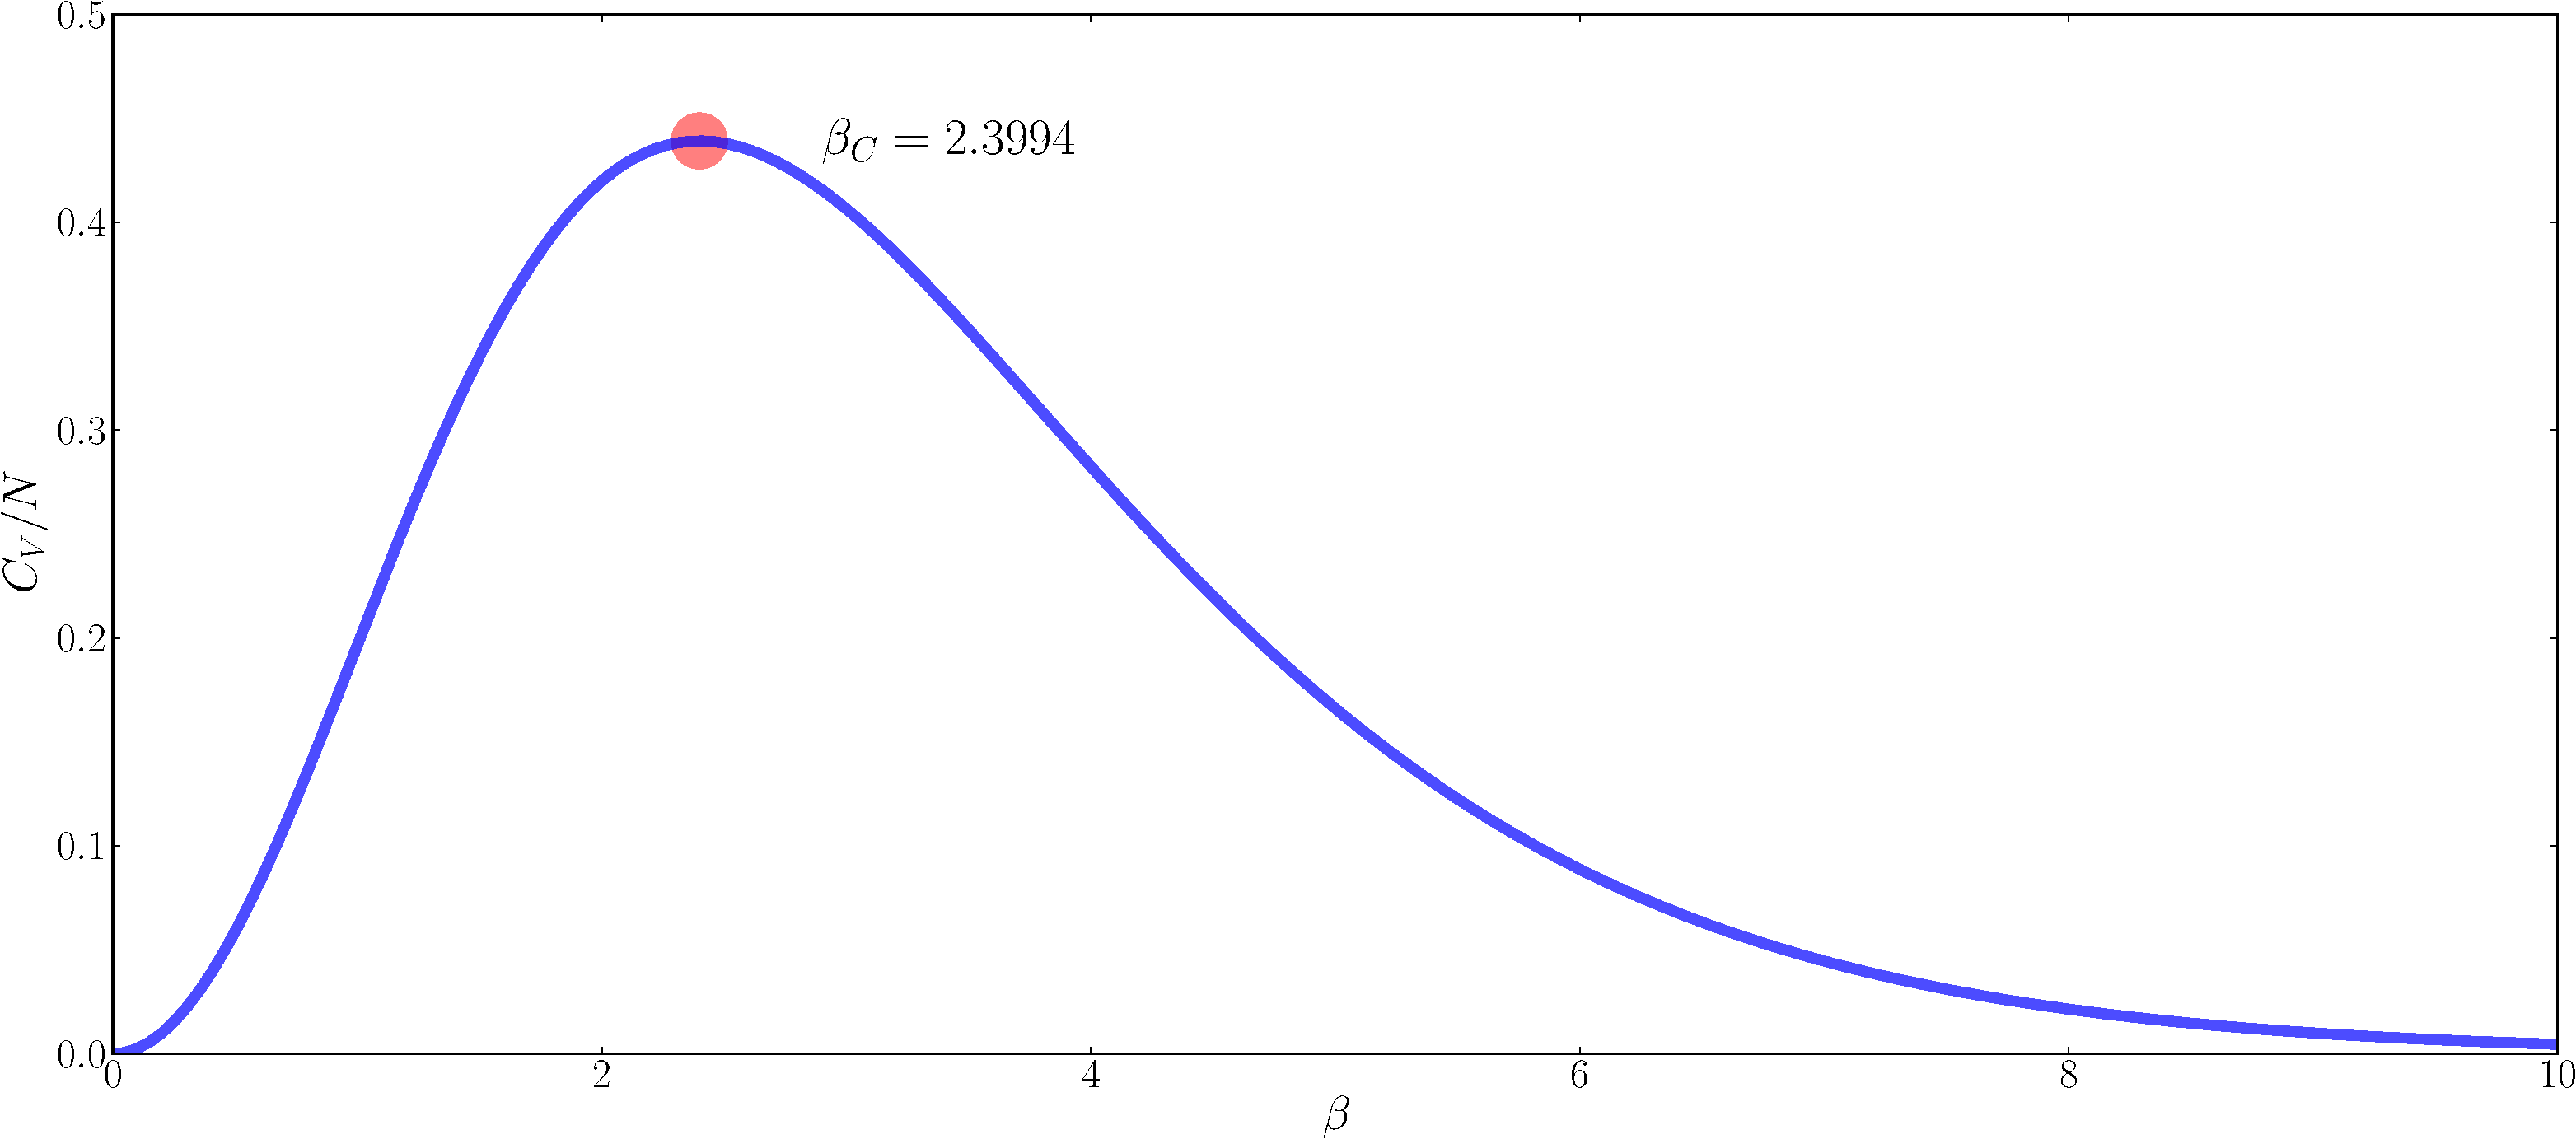
\includegraphics[width=.7 \textwidth]{pictures/1N_potts_ladder/pictures/CV_curve_potts_1N_ladder.pdf}
\caption{Specific heat per chain length for the one-dimensional Potts model with parameters $n=10^6$, $q=2$, and $J=-1$. The semi-critical $\beta$ was calculated from Equation \ref{eq:semi_critical_beta_potts_1N_ladder}. }
\label{fig:CV_curve_potts_1N_ladder}
\end{figure}
%

To visualize the behavior of the system on a larger scope, we can analytically continue the temperature onto the complex plane. In Figure \ref{fig:zeros_par_func_1n_ladder_no_field} we can visually inspect the behavior of the zeros on the complex plane. In the picture the semi-critical behavior (since we are plotting at finite $n$) is visible at $T=0$.

\begin{figure}[ht]
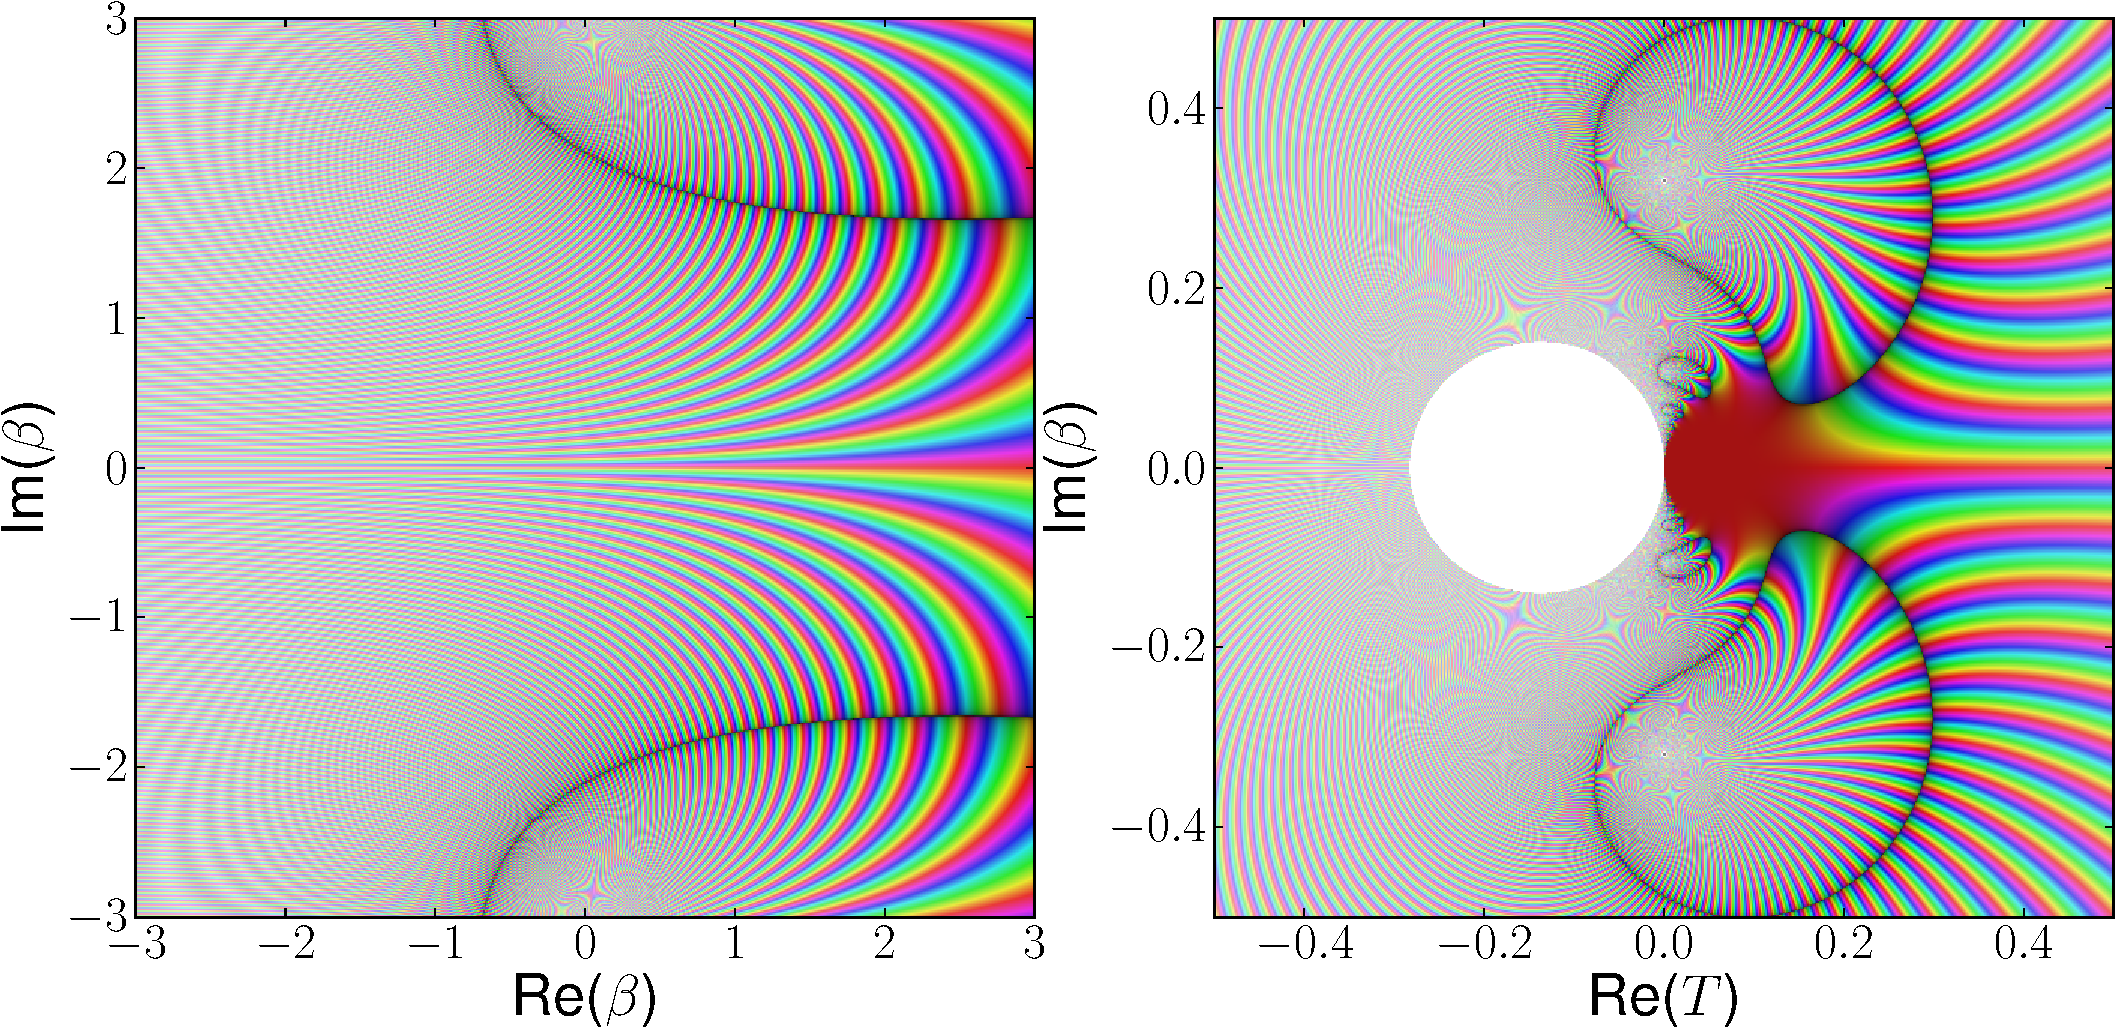
\includegraphics[width=\textwidth]{pictures/aggregation_model/pictures/zeros_parition_func_1N_ladder_2.pdf}
\caption{
Phase angle of the partition function for the $1N$ ladder with $J=-1$, $q=2$ where the temperature is continued onto the complex plane. The left plot has $\beta=1/kT$ to show the behavior of the high temperatures and the right plot shows the low temperature behavior. The points where the phase changes rapidly signify zeros of the partition function and hence first-order phase changes. The lighter areas on the low temperature plot are large values of the partition function (not zeros).
}
\label{fig:zeros_par_func_1n_ladder_no_field}
\end{figure}


\subsection{Special Case \texorpdfstring{$1N$}{1N} Ladder: Potts with Magnetic Field}

The standard Potts model with a field term only acting on the first state has the parameters of $w_j=w \delta(j,1)$ and $v_j=v$. This gives
\begin{align}
\CHI{a+1,}{a} 	&= w^{a+1}v^a + \sum_{j=2}^{q} v^a  
					 = w^{a+1}v^a + (q-1)v^a \\
X &= \sum_{n=0} y^n \CHI{n+1,}{n} 
   = {\frac{-w}{w v y-1}}-{\frac {q}{y v-1}}+ \frac{1}{y v-1}
\end{align}
Giving the generating function as
\begin{align}
Z(y) &=  {\frac { ( wvy-1 )  ( yv-1 ) }{{y}^{2}{v}^{2}w-y
v-w v y+1-w y+q w v{y}^{2}-y q+y}}
\end{align}
While resulting expression for $Z_n = \evalat{ \partial_y^n Z(y) } _ {y=0} $ is too complicated to evaluate explicitly, any particular term can be extracted with ease. 
\begin{comment}
To find semi-critical $\beta$ we look at the variance of the energy (where we substituted $v=e^{\beta J} -1$:
\begin{align}
\avg{ (\Delta E)^2 } &= 
\pfrac{^2 \ln(Z_n)}{\beta ^2} \\
&= {\frac { ( 1-q-n+nq ) {J}^{2}{{\rm e}^{\beta\,J}}}{ ({{\rm e}^{\beta\,J}}-1+q) ^{2}}}
\end{align}

Solving for the zeros of this function give:
\begin{equation}
\beta_c = \frac{\ln(q+1)}{J}
\end{equation}

Which when substituted into the specific heat $C_V = \beta^2 \avg{ (\Delta E)^2 }$, gives us the maximum value of the specific heat, a value independent of $J$ and $n$ for large values of $n$:
\begin{equation}
C_{V \text{max}} = \frac{\ln(q-1)^2 (n-1) }{4n} \approx \frac{\ln(q-1)^2 }{4}
\end{equation}

\end{comment}

\section{One-dimensional \texorpdfstring{$2N$}{2N}  Ladder }
\label{sec:two_d_ladder}

\begin{center}
\TIKZgraphtwoline
\end{center}

We give the general recurrence relation for the $2N$ ladder. The generating function solution remains an open problem. With a one dimensional strip two lattice units thick the operator is
\begin{equation}
\B{L} = 
\B{T}_{-2} \B{D}_2 \B{D}_1 
(\B{I} + \B{J}_{34}) 
(\B{I} + \B{J}_{13}) 
(\B{I} + \B{J}_{23}) 
\B{A}_{3} \B{A}_{4}
\end{equation}

There are now two general states which we have to consider. The first is when the vertices do not belong to the same partition $\ket{\pblock{1}{a_1}{b_1} \pblock{2}{a_2}{b_2} }$ and the second when they do belong to the same partition $\ket{\pblock{1 2}{a_3}{b_3}}$. We let $f_{a_1, b_1, a_2, b_2}$ and $g_{a_3, b_3}$ represent a shorthand for the two states respectively. The action of the operator is on $f$ is
\begin{align}
\B{L} f_{a_1, b_1, a_2, b_2} &= f_{a_1+1, b_1+1, a_2+1, b_2+1} 
											+ \CHI{a_1+1,}{b_1} f_{0,0, a_2+1, b_2+1} \\ \notag
                                	&+ \CHI{a_2+1,}{b_2} f_{a_1+1, b_1+1,0,0} 
                                	+ \CHI{a_1+1,}{b_1} g_{a_2+1,b_2+2} \\ \notag
                                	&+ \CHI{a_2+1,}{b_2} g_{a_1+1,b_1+2}
                                	+ g_{a_1+a_2+2,b_1+b_2+3} \\ \notag
                                	&+ \CHI{a_1+1,}{b_1} \CHI{a_2+1}{b_1} g_{0,1}
										  	+ \CHI{a_1+1,}{b_1} f_{0,0,0,0} 
\end{align}
And the action on $g$ is given by
\begin{align}
\B{L} g_{a_3, b_3}	&= f_{a_3+2, b_3+1, 0,0}
									+  f_{0,0,a_3+2, b_3+1} \\ \notag
									&+ 3g_{a_3+2,b_3+2}
									+  g_{a_3+2,b_3+3} \\ \notag
									&+ \CHI{a_3+2}{b_3} g_{0,1}
									+  \CHI{a_3+2,}{b_3} f_{0,0,0,0}
\end{align}
%
As before we let $\phi_n$ be the n\textsuperscript{th} application of $\B{L}$ against the initial state
\begin{equation}
\phi_n = \sum_{i,j \ge 0} c_{n, i, j} g_{i, j} + \sum_{i_1,i_2,j_1,j_2 \ge 0} d_{n, i_1,j_1,i_2,j_2} f_{i_1,j_1,i_2,j_2}
\end{equation}
with the initial state
\begin{equation}
\phi_0 = g_{0 1} + f_{0 0 0 0}
\end{equation}
We note that by symmetry we have
\begin{equation}
d_{n, i_1,j_1,i_2,j_2 } =  d_{n, i_2,j_2,i_1,j_1}
\end{equation}
%
Using that information we invert the equations
{
\allowdisplaybreaks
\begin{align}
c_{n01}&= \sum_{ij} \CHI{i+2,}{j} c_{n-1, i,j}   \\ \notag
		 &+ \sum_{i_1,i_2,j_1,j_2} \CHI{i_1+1,}{j_1} 
		 		\CHI{i_2+1,}{j_2} d_{n-1,i_1,i_2,j_1,j_2} \\ 
c_{nab} &= 3 c_{n-1, a-2,b-2} + c_{n-1, a-2,b-3} \\ \notag
		  &+ 2 \sum_{i,j} \CHI{i+1,}{j}  d_{n-1,i,j,a-2,b-2} \\ \notag
		  &+ 2 \sum_{i,j} d_{n-1,i,j,a-i-2,b-j-3} \\
d_{n a a00} &= c_{n-1, a-2,a-1} + S_1(a,a) + S_2(a) \\ \notag
d_{nab00} &= c_{n-1, a-2,b-1} + S_1(a,b) \\ \notag
d_{n,i_1,j_1,i_2,j_2} &= d_{n-1,i_1-1,j_1-1,i_2-1,j_2-1}
\end{align}
With
\begin{align}
S_1(a,b) &= \sum_{k=0}^{n-1} \CHI{k+1,}{k} d_{n-1-k,a-1-k,b-1-k,0,0} \\
S_2(a) &= \sum_{i=a}\sum_{j=a} \CHI{i+1,}{j} d_{n-a,i-a-1,j-a-1,0,0}
\end{align}
}

\section{Edge contraction methods}
\label{sec:edge_contraction_methods}

In the previous section we developed a method to determine the full partition function for an arbitrary graph with a field term using an operator expansion. While this is the most general method, it does limit the depth of the results one can obtain due to the complicated nature of the recursion relations. If we simplify the Hamiltonian by dropping the field term ($h=0$ in Eq. \ref{eq:potts_model_ham}), the solution to a wider class of graphs becomes tractable.

An equivalent evaluation to $\Z$ is the recursion relation mediated by graph reductions of edge contraction and removal (see Section \ref{sec:graph_introduction} for an explanation of these methods). There does not appear to be a general formula for the Potts model with an external field, but by relaxing this constraint there is the well-known relation\cite{godlin_graph_2008}
\begin{align}
\Z(G) &= w_{ij} \Z(G_{/ e_{ij}}) + \Z(G_{- e_{ij}}) \\
\Z(G_1 \sqcup G_2) &= \Z(G_1) \Z(G_2) \\
\Z(\emptyset) &= 1 \\
\Z(S) &= q
\end{align}
Here $/ e_{ij}$ is edge contraction, $-e_{ij}$ is edge removal, and $w_{ij}$ is the weight of the edge joined by vertices $i,j$. $G_1 \sqcup G_2$ represents two graphs that do not share any edges. $S$ is the singleton graph, with only one vertex and no edges and $\emptyset$ is the empty graph.

We can immediately derive the results for the $1N$ chain in the absence of an external field. As a pedagogical bonus, the resulting derivations can be done graphically. With a chain of length $n$, an edge weight of $v$ for each sequential vertex along the chain, the partition function for the n\textsuperscript{th} chain is
\begin{align}
Z(n) = \TIKZoneladderA
   & = v \paren{ \TIKZoneladderB }
+ \paren{ \TIKZoneladderC }
\\ \notag
& = v Z(n-1) + q Z(n - 1) 
\\ \notag
& = Z(n-1) (v + q)
\end{align}
%
Since the recursion relation is linear, it can be solved for in closed form giving exactly Equation \ref{eq:1N_ladder_potts_closed_form}.
\begin{align}
Z(n) &= q(v+q)^{n-1}
\end{align}

\subsubsection{$2N$ Ladder - Directional bonds}
We now attempt to solve the $2N$ chain with bond strengths that vary in along the short or long edge of the ladder. The strengths for the vertical and horizontal directions respectively are $J_1$ and $J_2$ (where $v_1=e^{J_1 \beta}-1$ and $v_2=e^{J_2 \beta}-1$)
{
\allowdisplaybreaks
\begin{align}
Z(n) &= \TIKZtwoladdera \\ \displaybreak[0]
     &= v_1 \TIKZtwoladderb + \TIKZtwoladderc \\ \displaybreak[0]
     &= v_1 v_2   \TIKZtwoladderd + Z(n-1) ( (v_2 + q)^2  + v_1(v_2 +q) ) \\ \displaybreak[0]
     &= v_1 v_2^2 \TIKZtwoladdere + Z(n-1) ( (v_2 + q)^2  + v_1(v_2 +q) + v_1 v_2 )  \\ 
     &= v_1 v_2^2  \TIKZtwoladderf  (1+ v_1) 
     + Z(n-1) ( (v_2 + q)^2  + v_1(v_2 +q) + v_1 v_2 )  
\end{align}
}
We notice however that the final graph is one that has already been seen before in the expansion, just shifted by one term in the recurrence
\begin{align}
Z(n-1)          &= v_1 \TIKZtwoladderf + Z(n-2) (v_2 + q)^2 \\
\TIKZtwoladderf &= \frac{1}{v_1} ( Z(n-1) - Z(n-2) (v_2 + q)^2) 
\end{align}
This gives the recursion relation of
\begin{equation}
Z(n) = Z(n-1)((q+v_2)^2+v_1(q+2v_2)) +  (Z(n-1)-Z(n-2)v_2^2 (q+v_2)^2(1+v_1)
\end{equation}
The initial conditions are
%
\begin{align}
Z(1) &= q(v_1 + q) \\
Z(2) &= ((v_1+q)(v_2+q))^2 - (v_1 v_2)^2 (q-1)
\end{align}
This again is a linear recurrence relation, albeit with two terms, that can be solved for rather easily. The closed form solution however is rather verbose and not particularly illuminating we provide the (slightly) more compact generating function
\epigraph{\begin{align}
Z(y) &= \frac{a}{b} 
\\ \notag a=& 
-y q(-y v_1v_2^2-y v_1v_2q-y v_1^2v_2-y q v_1^2-v_1-y q^2v_1-q+v_1^2v_2^2y+2y v_1v_2^2q
\\ \notag & \hspace{1em}
+ y v_1^2v_2q+y v_1v_2q^2+v_1^3v_2^2y+v_1^2v_2^2y q)
\\ \notag b=& 
v_1v_2^4y^2+v_1^2v_2^4y^2-2y v_2q-y v_1v_2-2y v_1v_2^2+1+2v_1v_2^3y^2q+2v_1^2v_2^3y^2q+
\\ \notag & \hspace{1em}
y^2v_1v_2^2q^2+v_1^2v_2^2y^2q^2-y v_1v_2q-y v_2^2-y q^2-v_1^2v_2^2y
\end{align}}{GF for 2N Ladder with no field term}

\begin{comment}
Using the closed form solution we can look for the discontinuities attempting to find phase transitions. The solutions for $v_1$ where $Z(n)=0$ are
\begin{align}
\text{critical}(v_{1c}) &=   
\{ -1, \rootof ((2v_2^2q+4v_2q+q^2+4v_2^2+v_2^4+4v_2^3)v_{1c}^2 + 
\\ \notag &
(-4v_2^3q+8v_2q^2-2q^2v_2^2+2q^3+12v_2^2q+8v_2^3)v_{1c}+4v_2q^3+4q^2v_2^2+q^4) \}
\end{align}
\end{comment}


Using the closed form solution we can look for the discontinuities attempting to find phase transitions. The solutions for $\beta$ where $Z(n)=0$ only have negative values for those on the real axis. It seems that the other roots also do not have real, positive solutions for $q \geq 2$, implying that the system has no mathematical phase transitions in the physical parameter space. This is best visualized in Figure \ref{fig:zeros_par_func_2nladder}.
%
\begin{figure}[hb]
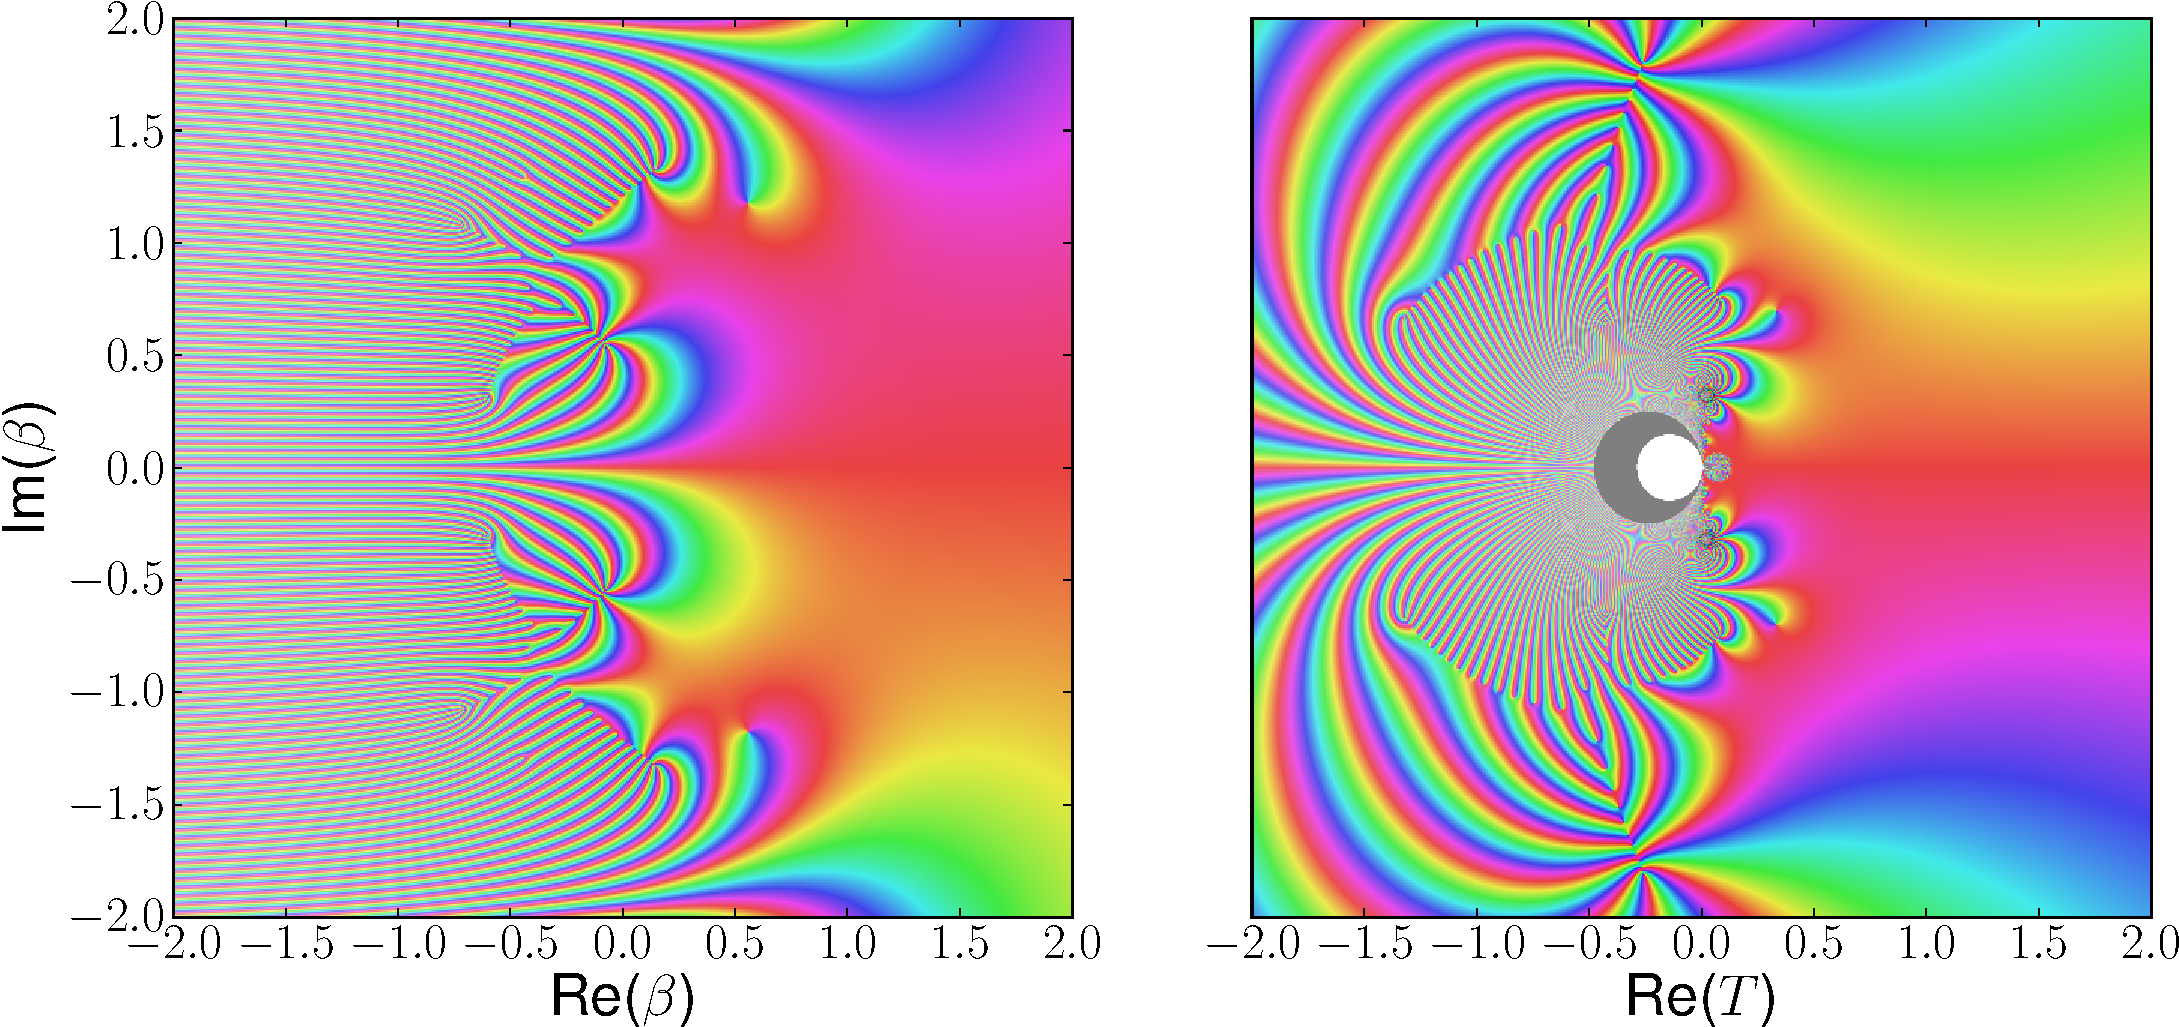
\includegraphics[width=\textwidth]{pictures/aggregation_model/pictures/zeros_parition_func_2N_ladder_2.pdf}
\caption{Phase angle of the partition function for the $2N$ ladder with $J_1=-2, J_2=-1$ where the temperature is continued onto the complex plane. The left plot has $\beta=1/kT$ to show the behavior of the high temperatures and the right plot shows the low temperature behavior. The points where the phase changes rapidly signify zeros of the partition function and hence phase changes. The gray areas and on the low temperature plot are large values of the partition function (not zeros) where the evaluation failed due to an overflow error. The lighter areas are large values of the partition function (not zeros).
}
\label{fig:zeros_par_func_2nladder}
\end{figure}

\begin{comment}
We can look at asymptotic large $n$ solutions by studying the poles of the generating function. The poles of the generating function $Z(y,n)$ are
\begin{align}
\{
\rootof (& 1+(v_2^4+v_2^4v_1+2v_2^3q+2v_2^3q v_1+q^2v_2^2+v_2^2q^2v_1)y_p^2
\\ \notag &
+(-2v_2^2-2v_2q-q^2-q v_1-2v_1v_2-v_2^2v_1)y_p)
\}
\end{align}
\end{comment}

\subsubsection{$3N$ Ladder - Directional bonds}
We give the general recurrence relations for a $3N$ ladder with bonds strengths that vary in direction. The strength for the vertical and horizontal directions respectively are again $J_1$ and $J_2$ where $v_1=e^{J_1 \beta}-1$ and $v_2=e^{J_2 \beta}-1$. It is to cumbersome to write the terms graphically in each equation, so we assign a symbol for each graph in the expansion indexed by the length of the ladder. 
{ \allowdisplaybreaks
\begin{tabular}{ c c c}
$Z(n)$            & $B(n)$               & $C(n)$ \\
\TIKZthreeladderA & \TIKZthreeladderB & \TIKZthreeladderC \\ 
$D(n)$               & $E(n)$               & $F(n)$ \\
\TIKZthreeladderD & \TIKZthreeladderE & \TIKZthreeladderF \\ 
$H(n)$               & $I(n)$               & $J(n)$ \\
\TIKZthreeladderH & \TIKZthreeladderI & \TIKZthreeladderJ \\ 
\end{tabular}
}
%
This gives a set of coupled recurrence relations
{ \allowdisplaybreaks
\begin{align}
Z(n) &= v_1 B(n) + (q+v_2) C(n) \\
C(n) &= v_1 D(n) + (q+v_2)^2 Z(n-1) \\
D(n) &= v_1 E(n) + (q+v_2) Z(n-1) \\
E(n) &= v_2(1+v_1) F(n) + Z(n-1) \\
B(n) &= v_1 G(n) + (q+v_2) D(n) \\
G(n) &= v_2 E(n) + (q+v_2)Z(n-1) + v_2 H(n) \\
H(n) &= v_2 I(n) + E(n) \\
I(n) &= v_2 (1+v_1)^2 G(n-1) + J(n) \\
J(n) &= v_1 (1+v_1) G(n-1)  + v_1 G(n-1) \\ \notag
     &\hspace{2em} + (v_2 + q)( Z(n-2)(1+ (v_2+q)) J(n-1) ) \\
F(n) &= B(n-1)
\end{align}
}
These equations could, in theory, be solved to get a recurrence relation on in terms of $\{ Z(n), Z(n-1), Z(n-2), \ldots \}$. We conjecture that the process could continue indefinitely for larger ladders, though we have not explored the $4N$ ladders or higher.

\section{Remarks}
%
In this chapter we developed new methods for solving the Ising/Potts model over arbitrary graphs and sought closed form solutions to ladder graphs. The ladder graphs have a natural connection to amyloid fiber aggregation with a preferred growth direction since one can take into account different bond strengths along each direction. These models permit only a few free parameters $J_1$, $J_2$, $q$ and for the graphs solved with external fields $h$. The results presented here open avenues of future work to connect the analytical models to concrete experimental data of real amyloid fiber growth by fitting these parameters.



  %CHAPTER: Clustering and Kinetics
  \chapter{Clustering and Kinetics}
\label{chap:clustering_kinetics}

Macrostates, collections of microstates that share similar characteristics, are a useful tool in the study of any system, for instance, in setting up coarse-graining models. For proteins in particular, with a small enough set of macrostates one can usually deduce the folding pathway with even a rudimentary kinetic model. This poses a problem for a system with many degrees of freedom; how does one go about finding the relevant macrostates in the first place? In this chapter we develop a plan for partitioning the microstates into broad, meaningful macrostates from time-series data or detailed microstate information. We begin with an outline of the methodology and elaborate on the details through two models: a kinetic trajectory taken from a frustrated Langevin system and a small, idealized $\beta$-hairpin embedded on a two-dimensional lattice. We will see that the macrostate clustering method developed here provides a robust tool in the analysis of dynamical systems. 

\section{Macrostate Clustering}
\label{sec:clustering_outline}

In theory, the equations of motion along with initial conditions impart complete knowledge of any system. In reality, the situation is more complex. Few systems can be solved analytically, and these solutions are often idealized models of the underlying mechanics. Topological characterizations can usually be made (such as Lyapunov exponents), but these convey a solution only in the broadest sense. What is needed is geometrical measure, a way of partitioning the phase space to a more manageable subset. If our system is near or at thermal equilibrium this is tantamount to  clustering the microstates into physically meaningful macrostates. The idea is not new, many of the early pioneers of biophysical models have been advocating different methodologies for macrostate classification.\cite{ozkan_computing_2003, zhou_minimum-reaction-flux_2008} It would be useful to have a general purpose algorithm for constructing the macrostates from information obtainable from the equations of motion, or a statistical description of the system.

In this chapter we propose a viable method for macrostate clustering (MSC for short). The MSC algorithm takes as input a kinetic trajectory and a single parameter. We convert the kinetic trajectory into a Markov matrix and use its eigenvectors to make this classification. Since an embeddable Markov matrix is a mapping from a system of linear first-order differential equations, the MSC algorithm can be considered a first-order approximation to the motion.

With a system specified by its Hamiltonian $\HAM$ and intensive properties, the first step is a suitable identification of the microstates $\{\xi_1, \xi_2,\ldots, \xi_N \}$. For continuous systems, the accessible state space must be partitioned.\footnote{In practice this is easily adjustable even after a trajectory has been obtained and does not change the results of the MSC algorithm greatly. With a finer partitioning method, more resolution is obtained at the cost of under-sampling. This consequently increases the running time.}  A trajectory is obtained by integrating the equations of motion, making note of the conformation at equal time intervals. An incidence matrix is formed by counting the number of times microstate $\xi_i$ moved to $\xi_j$. This matrix can be converted to a proper Markov matrix by normalizing the row sums. Alternatively, if one had complete knowledge of the microstates and the transition rates between them, one could convert this matrix into a Markov matrix without the loss of any information, that is, the Markov matrix is a snapshot of a continuous time Markov process. With Markov matrix $\B{M}$, compute the Schur eigendecomposition
\begin{equation}
  \B{M} = \B{V \Gamma V}^{-1}
\end{equation}
where $\B{\Gamma}$ is a diagonal matrix with  eigenvalues $\lambda_1 \geq \lambda_2 \geq \ldots \geq \lambda_N \geq 0$. Since $\B{M}$ is a Markov matrix, $\lambda_1=1$ corresponds to the slowest mode of relaxation of the system, \ie the steady-state. The other eigenvalues, being smaller, represent faster modes of relaxation (see Section \ref{sec:markov_matrix} for more details on Markov matrices). The influence of the modes on the relaxation of the system is exponential $\propto e^\lambda$, thus the slower modes not only represent the dominant flows of the system, they are less influenced by the initial conditions. This makes them prime candidates for macrostate discovery. The fastest mode included in this consideration is the single free parameter in the MSC algorithm, $\phi$. Let this parameter $0 \le \phi \le 1$ be the eigenvalue threshold cutoff. Take a cut of the eigenvector matrix $\B{V}$, retaining only those vectors where $\lambda_i > \phi$. At $\phi=1$ only steady-state is retained, while at $\phi=0$ all modes have equal influence.  If the number of eigenvalues remaining is $k$ then 
\begin{equation}
  \B{U} = \text{cut}(\B{V})
\end{equation}
is a $N$ by $k$ matrix. While the columns are the eigenvectors, each row $u_i \in \B{U}$ represents microstate $\xi_i$ contribution to the remaining modes. We call the vectors $u$ the eigenflows of the system. We can imagine each of the $N$ vectors as points in the space of $\mathds{R}^k$. This gives the central idea behind the MSC algorithm. Microstates should be grouped into macrostates by clustering their eigenflows. Eigenvectors are unique up to a sign, so the clustering must take this into account. Formally, we are looking to define a metric $\B{g}(u_i, u_j)$, such that two eigenflows belong to the same cluster if, for some small $\epsilon$ 
\begin{equation}
  \B{g}(u_i, u_j) = \norm{ u_i - u_j } < \epsilon
  \label{eq:egienflow_metric_general}
\end{equation}

The idea has physical appeal, points near a local minima in phase space should all have similar eigenflows. Transition points in the system should be different, they should split the flow across the boundaries giving distinct components in their eigenflows compared to the local minima. In practice we found the main stumbling block was twofold: the choice of a proper metric (Equation \ref{eq:egienflow_metric_general}) and a suitable algorithm to group the elements into clusters implied by $\B{g}_{ij}$. Initially we choose the Euclidean metric $\norm{\cdot}_2$ and used various clustering algorithms to group the states. The method was only partially successful. The greatest shortcoming was the introduction of several new ad-hoc parameters into the system from the clustering algorithms. We eventually settled on a simpler classification that relied on no new parametrization. Let
\begin{equation}
  \sgn(u) = \brackets{ \sgn(u_1),  \sgn(u_2), \ldots, \sgn(u_k) }
\end{equation}
be the sign signature of a vector, where we define 
\begin{equation}
\sgn(x) = \piecewisebrace{
 \begin{array}{r l l}
   -1 & : & x < 0 \\
    1 & : & x \ge 0 %\text{otherwise}
 \end{array}
 }
\end{equation}
%
Two microstates belong to the same cluster (and hence macrostate) if and only if their sign signatures are equal. We assign each of the microstates $u_i$ to clusters in $\mathcal{C}^\prime = \braces{ c_1, c_2, \ldots, c_{2^k}}$. Not every cluster will be populated, since it is possible for $2^k > N$. Let $\mathcal{C}$ be the set of non-empty clusters and $\abs{\mathcal{C}}$, $\abs{c_i}$ count the number of clusters and the number of microstates within cluster $c_i$ respectively.

\subsection{Quasi-steady-state}

Once the clusters have been identified, we can present a macroscopic version of the original Markov matrix. Since macrostate behavior is often dominated by rare transitions between macrostates, we will assume that each macrostate relaxes to a local steady-state. We call this the quasi-steady-state. For each cluster we first compute the quasi-steady-state transition probability. 

Let $\B{M}_{c_i}$ be the square matrix with $\abs{c_i}^2$ elements that are pulled from cluster $c_i$.
This cluster is approximated as an isolated system, as we've only retained the flows within this cluster. We row normalize the matrix, discarding any rows (and their associated column) where the row sum is zero. Such states are possible within a transient cluster since it is conceivable that the trajectory from a fixed microstate does not flow to any other microstate in the cluster. The quasi-steady-state vector $\pi(c_i)$ is given by the left-eigenvector with eigenvalue one of the reduced renormalized Markov matrix
\begin{equation}
  \pi(c_i) \B{M}_{c_i} = \pi(c_i)
\end{equation}

Once we have computed the quasi-steady-states we use them as initial conditions to approximate macrostate behavior. Over a single time step these initial conditions will flow into other clusters giving us macrostate kinetics. Let $b_i$ be a vector of initial conditions from the full system. This vector has $N$ elements that correspond to those in $\pi(c_i)$, \ie it is the initial condition of quasi-steady-state for cluster $c_i$ and zero for all the elements of the other clusters. We start the system in $b_i$ and advance it one time step $b_i \B{M}$ to get the Markov macrostate matrix $\B{S}$.
%
\begin{equation}
  \B{S}_{a b} = 
  \sum_{i \in c_b}^{\abs{c_b}} 
  \paren{ b_a \B{M} }_{i} 
  \label{eq:macrostate_cluster_matrix}
\end{equation}

The matrix $\B{S}$ gives us new macrostate information. In addition to simply identifying the macrostates, the matrix identifies kinetic pathways by giving us the transition rate to each cluster. By starting at some set of initial conditions, we can trace a pathway along the clusters by continuously applying $\B{M}$ to the set. From here we can discard irrelevant clusters to a particular problem, and identify intermediate macrostates along the way. The identification of intermediates would be difficult with the original matrix; no single intermediate microstate dominates the statistics. When the states are clustered together, their similar eigenflows tend to move in tandem. These newly identified macrostates could present a new reaction coordinate or kinetic pathway. In the two subsections below, we apply the formalism to two illustrative cases.

\section{Frustrated Langevin Walk}

In this example we work directly with time-series data from a kinetic trajectory. The trajectory is obtained by integrating the equations of motion of a random walk in an external field. We will see that only the time-series data are needed, knowledge of the Hamiltonian or a suitable reaction coordinate is not required to determine the macrostate classification.  This example is particularly useful in view of the popularity of molecular dynamics (MD) simulations in the biophysical community.\cite{karplus_molecular_2002} In MD simulations, one often has many degrees of freedom, hence developing a general model is often a non-trivial task. The ability to partition the conformational space into physically relevant macrostates of lower dimension would greatly facilitate a deeper understanding of the system.

We model a particle in a viscous fluid subject to stochastic noise in a Langevin-like equation.\cite{coffey_langevin_2004} There are kinetic traps - minima in the potential that localize the motion until the particle can escape by thermal diffusion. Because of this, we call the system a frustrated Langevin walk (FLW). 

The traps are modeled as Gaussian wells. To simplify the expression of the equations of motion we define an isotropic Gaussian well that is centered at $(x_R, y_R)$ by 
\begin{align}
  L(x_R,y_R) &= -\exp \paren{ - \sqrt{ (x-x_R)^2 + (y-y_R)^2 } } \\
  \intertext{The potential, shown in Figure \ref{fig:clustering_smooth_map_traj}, is the contribution of three wells}
  V(\B{x}) &= L(0,0) + L(2,2) + L(0,-2)
  \label{eq:FLW_potential}
\end{align}
with $\B{x} =(x,y)$. Since the potential at a given point is the sum of the Gaussian wells, the depth at each of the three minima have the relation $V(0,0) < V(0,-2) < V(2,2)$. 

In addition to the potential, the particle is subject to stochastic noise and viscous damping
%
\begin{equation}
  m \B{\ddot x} = - \nabla V(\B{x}) - \lambda \B{\dot x} + \B{\eta}(t)
  \label{eq:FLW_force_eq}
\end{equation}
The dot notation indicates a derivative with respect to time. The damping coefficient  $\lambda$, is a measure of the frictional forces acting on the system proportional to the velocity. The stochastic term $\B{\eta}$, is an approximation to the microscopic collisions the particle would experience in a real fluid. The force has a correlation time of
\begin{equation}
  \avg{ \eta_i(t) \eta_j(t') }
  =
  \frac{ 2 \lambda }{\beta} \delta_{i,j} \delta(t- t')
\end{equation}
%
We choose the parameters $\beta=m=1$, $\lambda=0.07$ as they were sufficiently weak to bound the motion, but strong enough to occasionally facilitate a transition over the potential barriers. We integrated the system for a total time of $t_{\text{max}} = 10^6$ using a time step of $\Delta=0.2$ with a standard Runge-Kutta 4th order integrator.\footnote{
  Integrating a stochastic differential equation properly is a subtle, difficult task. Since most integration schemes rely on a Taylor expansion, it becomes problematic when there are force terms that are nowhere differentiable. In general, one must expand with the time-ordered exponential $T$
  \begin{equation}
    T \brackets{\exp{
        i \int_0^{\delta t} \mathcal{L}(s) d s 
    }}
  \end{equation}
  where $\mathcal{L}$ is the Liouvillian.\cite{suzuki_general_1992} Since our focus is on the method of macrostate approximation, we estimate the stochastic force by adding a random perturbation to the force each step of the integration. A deeper study of the system in question would require a proper handling of this issue by considering a suitable time-ordered integration scheme.\cite{goldman_nth-order_1996, ricci_algorithms_2003,ciccotti_deterministic_2004}
} 
%
The trajectory $\mathcal{T}$, is an ordered list
\begin{equation}
  \mathcal{T} = \{ \B{x}_{t_0}, \B{x}_{t_1}, \ldots, \B{x}_{t_\text{max}} \}
\end{equation}
%
A sample trajectory is plotted in Figure \ref{fig:clustering_smooth_map_traj}. The accessible coordinate space $\{\xi_1, \xi_2,\ldots, \xi_N \}$, is given by discretizing the interval $\B{x} \in [-4,4]$ into $N=45^2$ squares . For a given position, let $\Xi(\B{x})$ return the discretized position in coordinate space. For example, if $\B{x}_i \in \xi_j$ then $\Xi(\B{x_i}) = \xi_j$. We choose a lag time of $5 \Delta$ to simulate the collection of time-series data collected at larger intervals than the integrating time-step. Next we computed an incidence matrix $\B{C}_{ij}$. This matrix counts the number of times over the lag time the trajectory went from $\xi_i$ to $\xi_j$ 
\begin{equation}
  \B{C}_{ij} = 
  \sum_{i=5}^{ {t_{\text{max}}}/{\Delta}} \delta(\Xi(\B{x}_{t_{k-5}}),  \xi_i) \ \delta(\Xi(\B{x}_{t_{k}}),  \xi_j)
\end{equation}
%
A Markov matrix $\B{M}$ is constructed from the incidence matrix by normalizing the row sums
\begin{equation}
  \B{M}_{ij} = \frac{ \B{C}_{ij} } {\sum_k \B{C}_{kj}}
\end{equation}
%
It is worth nothing that the resulting Markovian matrix is only a linear approximation to the actual dynamics. Especially in the regions between pairs of the wells the may not hold. However, it is a useful first-guess a the transition rates that can later be refined. The Markov matrix was diagonalized and clusters were created with an eigenvalue cutoff of $\phi = 0.85$. This partitioned the conformational space into four clusters, shown in Figure \ref{fig:clustering_smooth_map_cluster_loc}.

\begin{figure}[tb]
  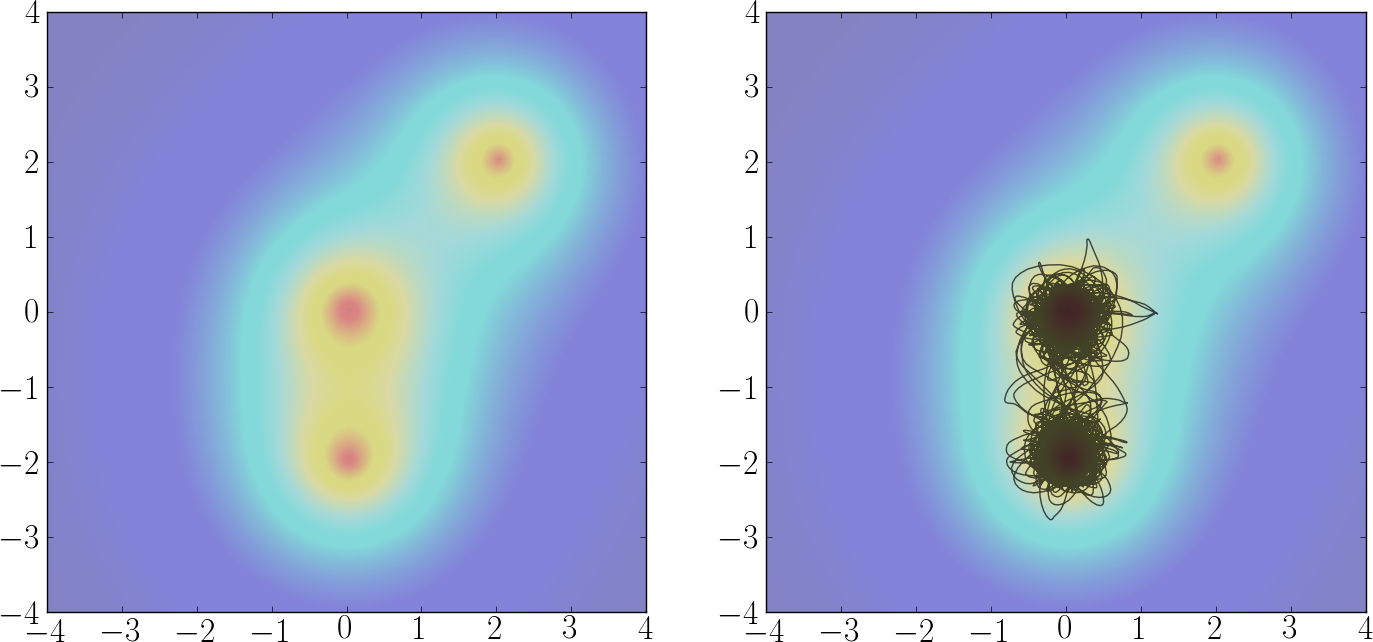
\includegraphics[width=.8\textwidth]{supplement/smooth_potential_cluster/pictures/smooth_potential_traj.png}
  \caption{(Left) Contour map of the three well Gaussian potential, Equation \ref{eq:FLW_potential}. (Right) A sample ($0.2 t_{\text{max}}$) of the FLW trajectory shown by integrating Equation \ref{eq:FLW_force_eq}. The motion is localized in the wells, escaping only when random fluctuations push it over a potential barrier.}
  \label{fig:clustering_smooth_map_traj}
\end{figure}
%
With the clusters identified, we permuted the Markov matrix to reflect our knowledge of the clusters. In Figure 
\ref{fig:clustering_smooth_map_markov_permutes} we see that the original matrix has no particular structure, while the permuted matrix shows a nearly block diagonal structure. The non-zero elements off the block diagonal indicate transitions between the clusters, while those within the block indicate movement within the cluster. The macrostate approximation identified all three local minima and the largest crossing barrier. Our choice of $\phi$ was not arbitrary, it was selected to be large enough to grab the semi-stable states, yet small enough to have broad macrostates. When $\phi$ is lowered, the state space partitioned into finer clusters. This may or may not be helpful in determining a kinetic pathway, the macrostates need to be connected to a physically relevant set of macro coordinates. Therefore, while a lower $\phi$ gives more information, not all of it is useful. For example, when a slightly lower $\phi$ is used there are two new macrostates: the first is a barrier crossing between the bottom wells (labeled $c_1$ and $c_2$ in Figure \ref{fig:clustering_smooth_map_cluster_loc}), and the second is a ring shaped boundary around the upper well $c_0$. The first is well-understood, it clearly represents the boundary between two more dominant macrostates; this barrier is useful for characterizing the system. The second is also easy to explain; there is simply a transient state that moves away from the top cluster only to quickly return. However, knowledge of this transient state does little to further our understanding of the system. Thankfully the cluster calculation is quick compared to the generation of time-series data for even a modest system. 

\begin{figure}[tb]
  \begin{center}
    \begin{tabular}{c c}
      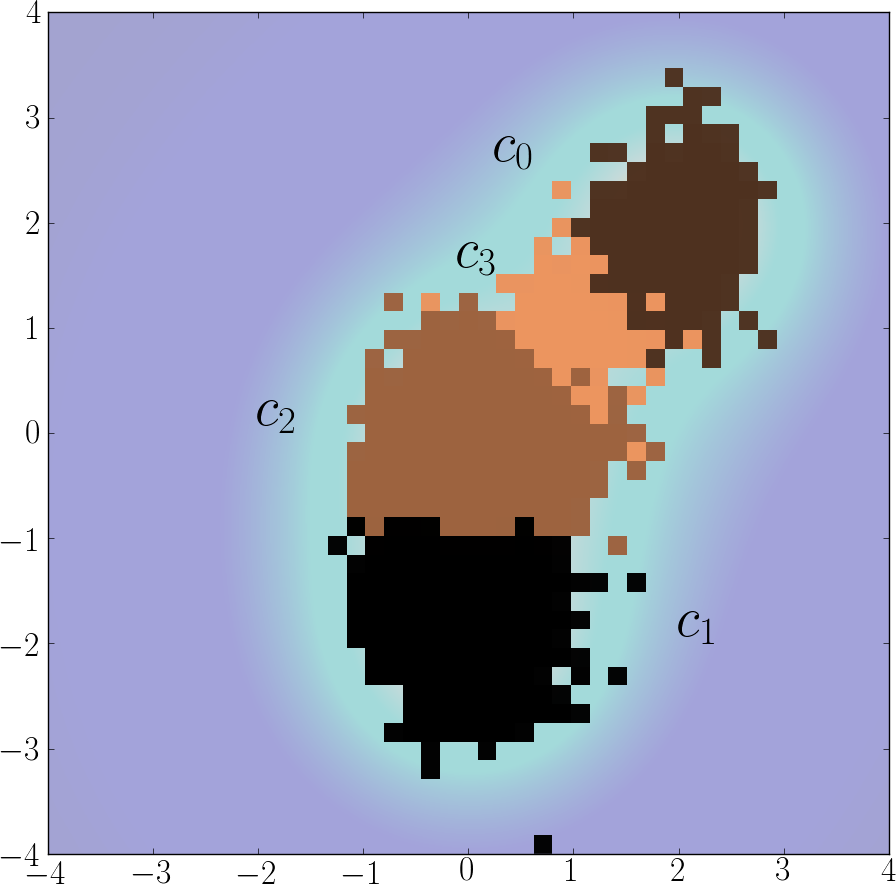
\includegraphics[width=.5\textwidth]{supplement/smooth_potential_cluster/pictures/cluster_locations.png}
    \end{tabular}
  \end{center}
  \caption{ Clusters found by partitioning the eigenflows of the FLW trajectory (Equation \ref{eq:FLW_force_eq}). Here $c_i(n)$ denotes the i\textsuperscript{th} cluster with $n$ conformational states in it. The original potential is overlaid. The algorithm found all three potential minima and identified a section as a crossing barrier.}
  \label{fig:clustering_smooth_map_cluster_loc}
\end{figure}
%
\begin{figure}[tb]
  \begin{center} \begin{tabular}{c c}
      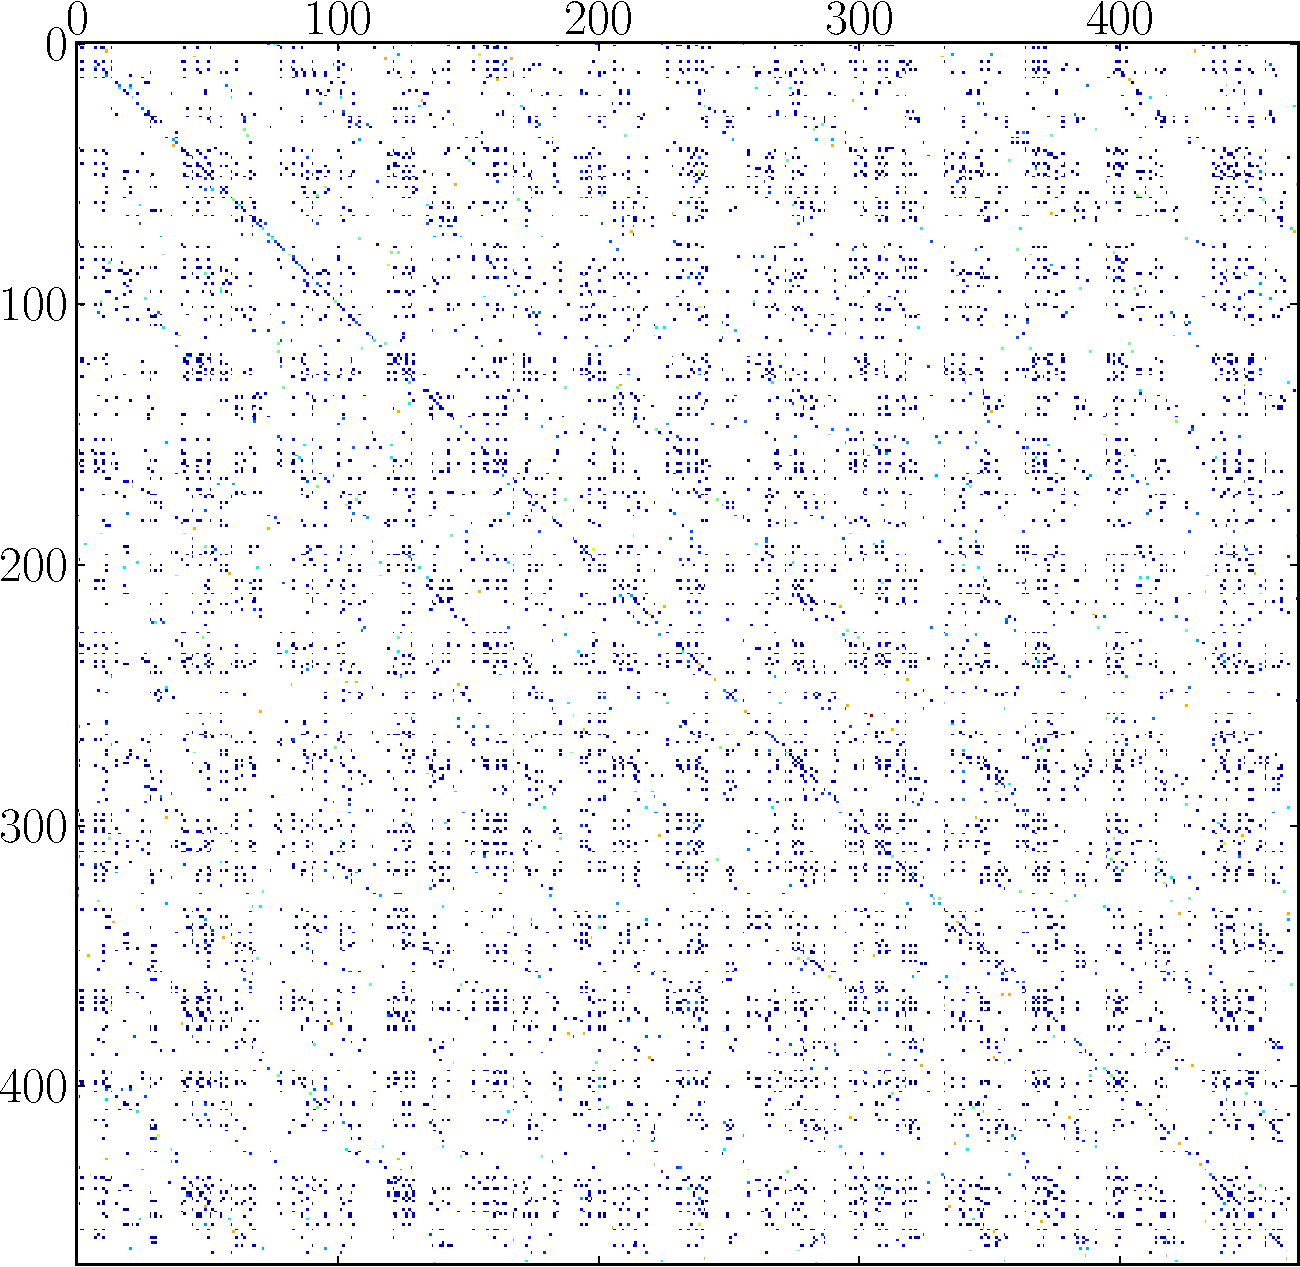
\includegraphics[width=.35\textwidth]{supplement/smooth_potential_cluster/pictures/markov_matrix_unpermuted.pdf}
      &
      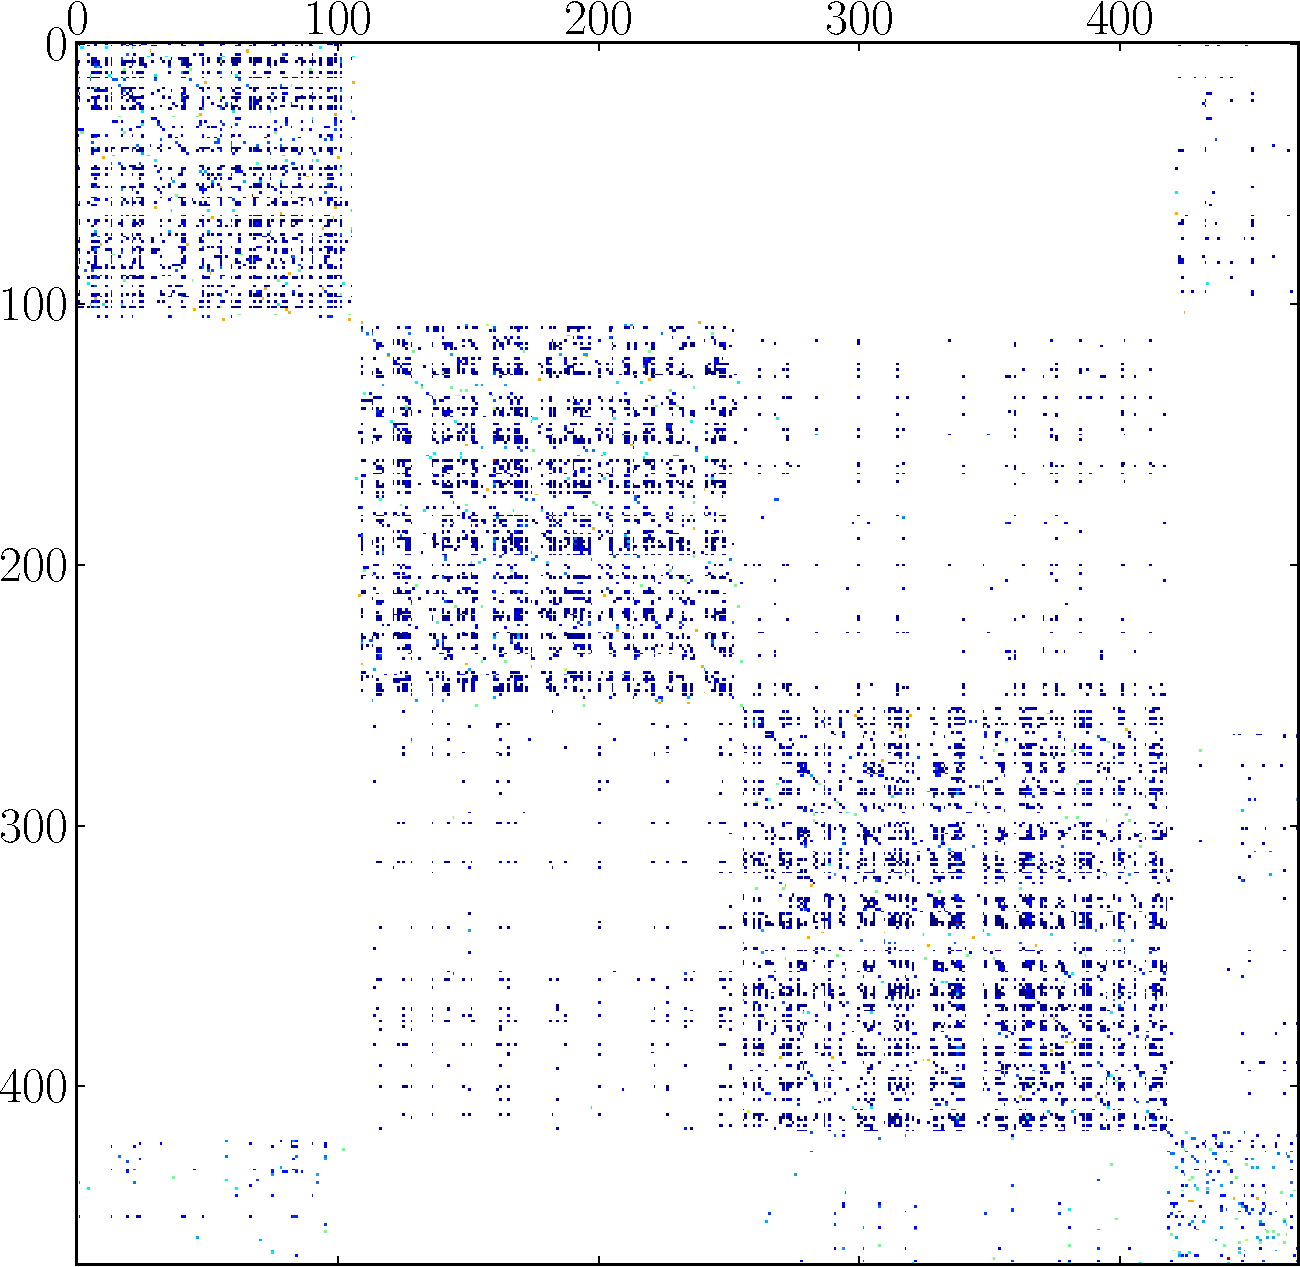
\includegraphics[width=.35\textwidth]{supplement/smooth_potential_cluster/pictures/markov_matrix_permuted.pdf}
  \end{tabular} \end{center}
  \caption{Markov transition matrix for the FLW system. The left matrix shows the states in the original, unsorted form. On the right the states have been permuted such that the states that belong to the same cluster are in adjacent rows. The block diagonal structure is clearly evident. }
  \label{fig:clustering_smooth_map_markov_permutes}
\end{figure}
%

To reduce the degrees of freedom of the system, we suggest a new kinetic pathway. With the above choice of $\phi$, all clusters have physical significance. Clusters $c_0$, $c_1$, and $c_2$ are the local minima while cluster $c_3$ is a barrier. Our model should reflect the kinetics of these four macrostates. We first computed the macrostate kinetic matrix $\B{S}$ from Equation \ref{eq:macrostate_cluster_matrix} by solving for the quasi-steady-state flows. This matrix was converted into  a rate transition matrix by the relation\footnote{
While one can compute the logarithm of a matrix, there are issues such as  embeddability and uniqueness that do not occur in the matrix exponential. Matrix $\B{A}$ is said to be embeddable if there exists a matrix $\B{B}$ such that $\B{A} = \exp(\B{B})$ and $\exp(t \B{B})$ is Markov for all $t \ge 0$. This is equivalent to taking a snapshot of an autonomous finite state Markov process that evolves continuously in time.\cite{davies_embeddable_2010} In addition, the matrix logarithm is not necessary unique. If the matrix is diagonalizable and the spectrum of eigenvalues are all strictly greater than zero, than the logarithm is unique and is given by $\log \B{A} = \B{V} \log (\B{\Gamma}) \B{V}^{-1}$. This is the Schur decomposition where the logarithm is applied to the diagonal matrix of eigenvalues. For the FLW walk, the matrix $\B{S}$ satisfied both constraints, hence the rate matrix obtained was unique.
} $t \B{W} = \log \B{S}$ giving
%
\begin{equation}
  t \B{W}_\text{reduced} = 10^{-4}
  \begin{bmatrix}
    -29  &  &  & 29 \\
    & -61 & 61 &  \\
    & 37 & -41 & 4 \\
    3181 &         & 1198 & -4377 \\
  \end{bmatrix}
\end{equation}
%
For clarity, blank entries are zero. Taking the entries of this matrix, we can now propose a simple discretized linear model for the movement in the conformational space.
%
\inlinembox{Macrostate model for FLW\vspace{.5em}}{\TIKZFLWmacrostates}
%
The macrostate characterization is complete. A new reaction coordinate for the system is suggested by this model, one that moves along the average coordinates for each macrostate. Since the macrostates are only approximations deduced from trajectories, their primary use is a categorical tool. One can also estimate first-crossing times and other kinetic predictions using various classical reaction-rate theories.\cite{haenggi_reaction-rate_1990} 

\FloatBarrier

%----------------------------------------------------------------------------------------------------------------------------

\section{Folding Pathway of a Beta-Hairpin}
%
For our second example illustrating an application of the MSC algorithm, we choose a system where the evaluation of the macrostates is not as straightforward as the FLW. Here the microstates are the various conformations of a simple lattice peptide. For a peptide, coarse-graining of the conformational space is usually achieved by various reaction coordinates such as fraction of native contacts or radius of gyration. These are selected with an \emph{a posteriori} knowledge of the physical and relevant coordinates. Here we profess ignorance of the system to see if the MSC algorithm can help determine a proper reaction coordinate. 

The general properties and behavior of lattice peptides have been detailed in the previous chapters (\cf Section \ref{sec:methods}). The peptide in our current study is constructed such that it displays both an interesting folding pathway and is a reasonable approximation to the known folding properties of a ten residue $\beta$-hairpin. Each of the ten residues has a property $r_i \in \braces{\chem{H}, \chem{P}, \chem{C_+}, \chem{C_-}, \chem{N} }$ in a \chem{H P C} bead-model Hamiltonian (hydrophobic, hydrophilic, charged residues) where $\chem{N}$ is a neutral non-interacting residue. Two residues in contact on the lattice contribute to the Hamiltonian
%
\begin{align}
  \HAM &= \sum_{i} \sum_{j>i+3} \delta(v_i,v_j) \paren{
    E_\chem{HP}(i,j) +  E_\chem{H H}(i,j) + E_\chem{PP}(i,j) +  E_\chem{C_+ C_-}(i,j) 
  }
\end{align}
Here $\delta(v_i, v_j)$ is $1$ if and only if residues $v_i$ and $v_j$ are nearest neighbors on the lattice. The energies $E_\chem{AB}$ are defined by an interaction strength $\epsilon_{\chem{AB}}$ and are non-zero if and only if residues $v_i$ and $v_j$ have the property $\chem{AB}$ (the ordering is unimportant). The magnitudes of the various interactions are
\begin{align}
  \epsilon_\chem{H P}      &= 0.1  \\ \notag
  \epsilon_\chem{P P}      &= -0.5 \\ \notag
  \epsilon_\chem{H H}      &= -0.6 \\ \notag
  \epsilon_\chem{C_+ C_-}  &= -1.5 
\end{align}
%
A picture of the unique native state is shown in Figure \ref{fig:betahairpin_nativestate}, with energy $-3.2$. This lattice Hamiltonian is one of the simplest $\beta$-hairpin models possible that captures the biological essence, namely:
%
\begin{itemize}
\item Favorable turn formation: One of the defining observed characteristics of the hairpin is the favorable internal energy the residues make at the turn. This is primarily due to the formation of a salt bridge. 
\item Realistic relative energetic magnitudes: The energies are chosen such that $- \epsilon_\chem{HP} < \epsilon_\chem{P P} < \epsilon_\chem{H H} < \epsilon_\chem{C_+ C_-}$.
\item Hydrophobic core: By including some unfavorable $\chem{HP}$ interactions we define a clear hydrophobic core that stabilizes at the center of the protein. In addition, this creates an enthalpic barrier to reach the unique native state if the protein misfolds.
\end{itemize}
%
\begin{figure}[tb]
  \TIKZbetahairpinNativestate
  \caption{Native state of the ten residue two-dimensional lattice $\beta$-hairpin. Residues marked with \chem{H}, \chem{P}, \chem{C+}, \chem{C-}, \chem{N} are hydrophobic, hydrophilic, charged, uncharged and neutral respectively.}
  \label{fig:betahairpin_nativestate}\end{figure}

Previously we've seen that sampling the state space can be done efficiently with Monte-Carlo techniques. In this case however, the state space is small enough to enumerate completely. Accounting for rotational and mirror-image symmetries there are only $N=714$ possible conformations of the system. The conformations are linked to each other by a move set of rigid rotations; every point on the chain was a permissible pivot to a new conformation as long as the resulting chain did not self-intersect. Since the chain length is less than $12$, it is known that rigid rotations for a two-dimensional lattice peptide provide sufficient ergodicity.\cite{chan_effects_1990} Numbering the conformations $\Xi=\{ \xi_1, \xi_2, ..., \xi_N \}$ we define an adjacency matrix $\B{A}$, where $\B{A}_{ij}=1$ if and only if conformation $\xi_j$ can be reached from conformation $\xi_i$ by exactly one rigid rotation.

We compute the transition rate from two states using both Metropolis and Glauber dynamics.\cite{glauber_time-dependent_1963} In both methods one needs to compute the energy difference $\Delta E_{ij} \equiv \HAM(\xi_j) - \HAM(\xi_i)$. For $i \neq j$ the transition rate matrix is specified by
\begin{itemize}
\item Metropolis dynamics
  \begin{equation}
    \B{W}_{ij} = \min (1, e ^{-\beta \Delta E_{ij}  }  )
    \label{eq:metro_dynamics}
  \end{equation}
\item Glauber dynamics
  \begin{equation}
    \B{W}_{ij} = \frac { e ^{-\beta \Delta E_{ij}}}  { 1 + e ^{-\beta \Delta E_{ij}} }
    \label{eq:glauber_dynamics}
  \end{equation}
\end{itemize}
For $i=j$, $\B{W}_{ii} = - \sum_{k \neq j} \B{W}_{kj}$ (see Section \ref{sec:master_equations} for additional details on the master equation formulation). We take the exponential of this matrix to get a Markovian one, $\B{M}=\exp (t \B{W})$ with $t=0.5$ and $\beta=4$. While different rates were obtained using Glauber and Metropolis dynamics, there was no discernible difference in the results of the MSC algorithm. As in the previous problem with the FLW system, we show the original and permuted Markov matrices in Figure \ref{fig:Rate_Matrix_Permutations}. The block diagonal structure can be seen for small isolated clusters, but a large majority of conformations reside in the large block. Examining the states in this cluster we see that these are the random coil states. 
\begin{figure}[tb]
  \begin{center}
    \begin{tabular}{c c}
      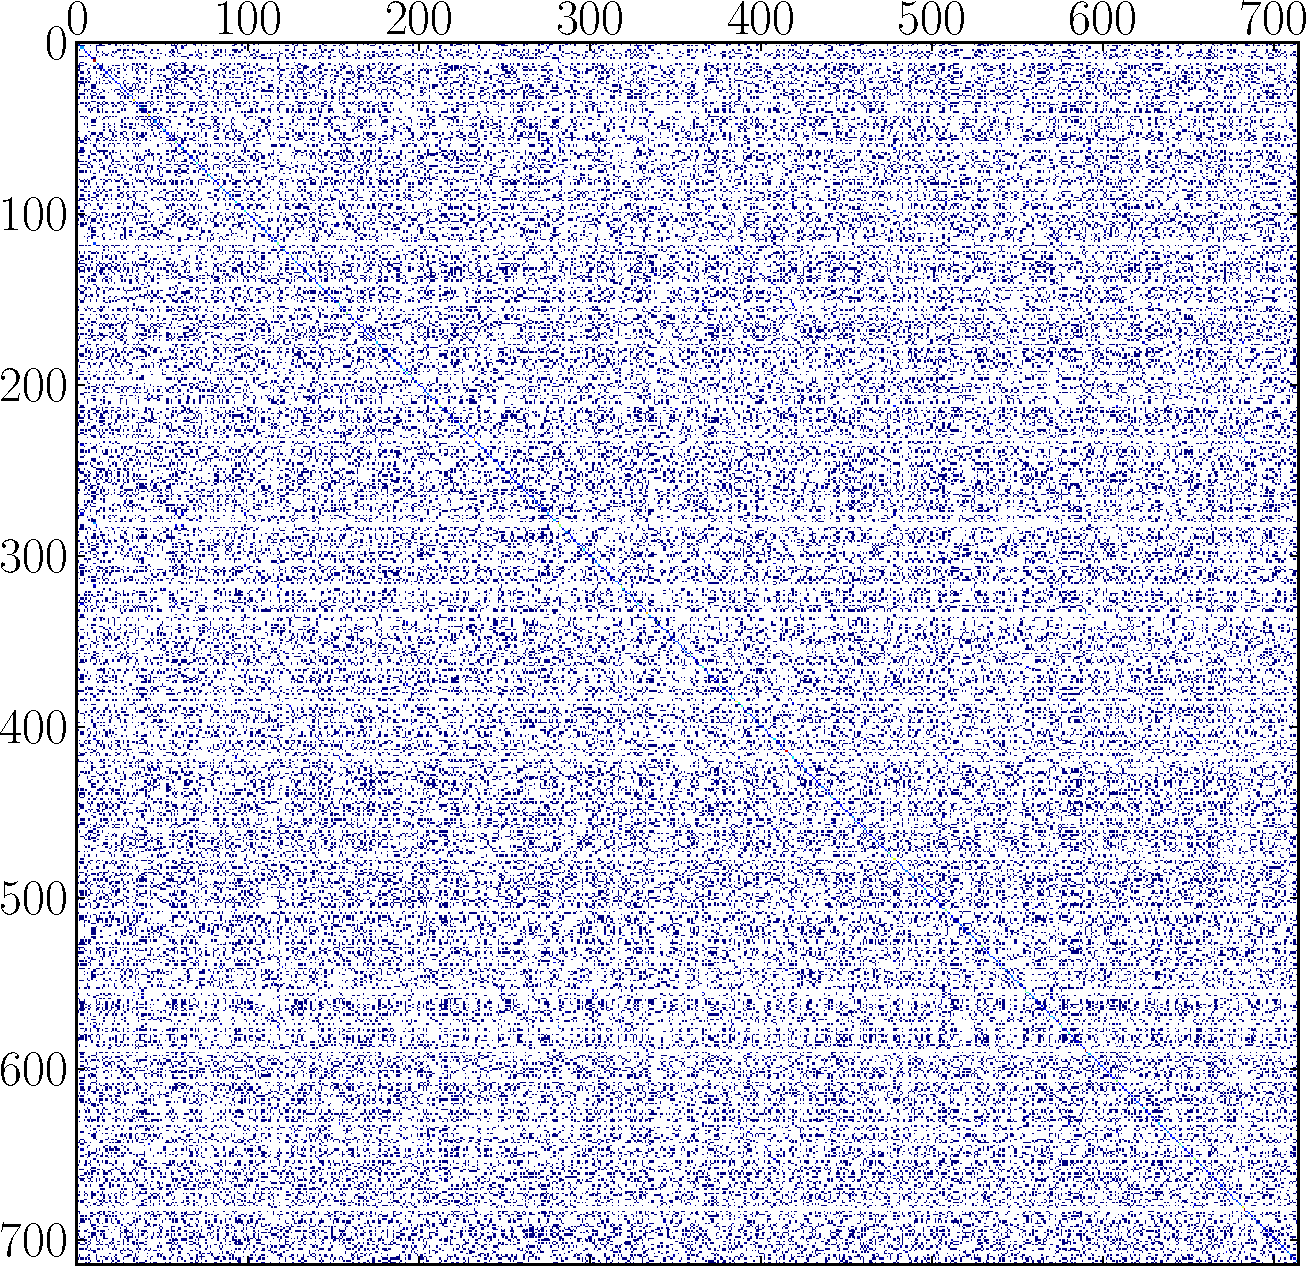
\includegraphics[width=.35\textwidth]{supplement/beta_cluster_example_2/pictures/markov_matrix_unpermuted.pdf}
      &
      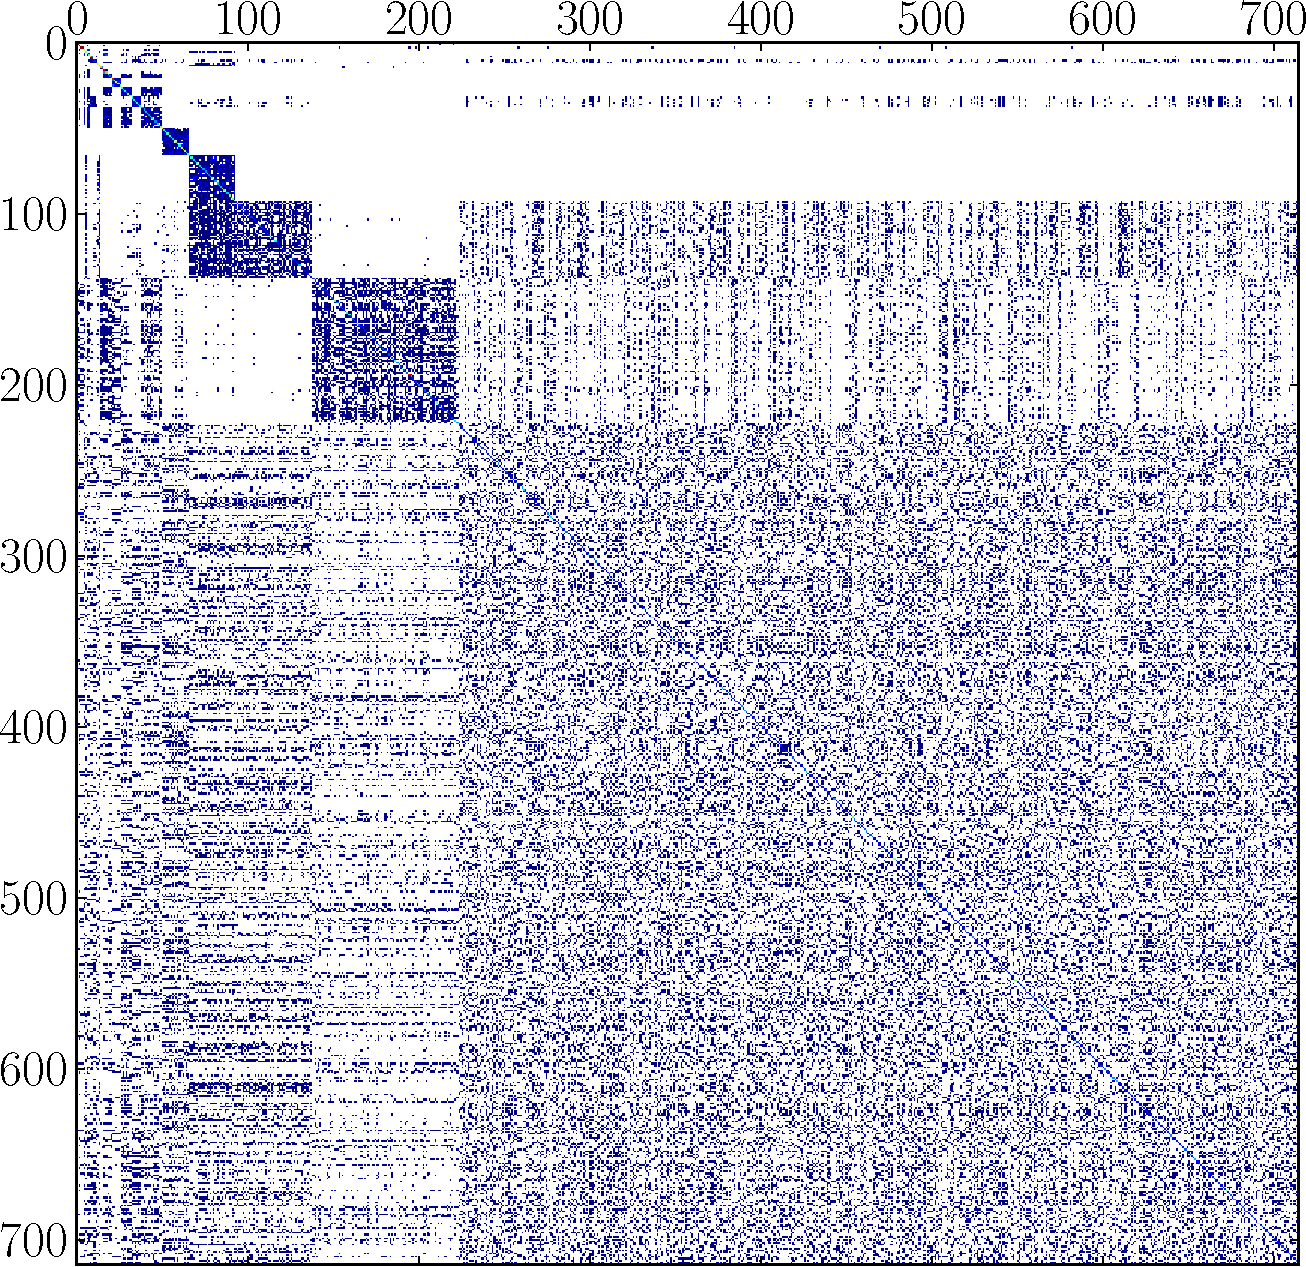
\includegraphics[width=.35\textwidth]{supplement/beta_cluster_example_2/pictures/markov_matrix_permuted.pdf}
    \end{tabular}
  \end{center}
  \caption{Markov transition matrix for the $\beta$-hairpin system using Glauber dynamics. The left matrix shows the states in the original, unsorted form where the states were enumerated by rigid rotations. On the right, the matrix has been permuted such that the states that belong to the same cluster are in adjacent rows. The block diagonal structure is clearly evident, with a large fraction of the states grouped into a single cluster. }
  \label{fig:Rate_Matrix_Permutations}
\end{figure}

\subsection{Folding Nucleation}
In this system there were $22$ identified clusters, though not all of them were physically relevant. To see why, we start the system in an initial state of the fully extended random coil $b_c$. We advance the system in time via $b_c \B{S}^t$ and plot the occupational probabilities of the clusters. In Figure \ref{fig:beta_hairpin_kinetics} we see the long-time behavior of the system. In the figure we order the clusters by the number of microstates they contain to illustrate the magnitude of the largest cluster. The ordering of the clusters is unimportant, any permutation would give the same macrostate information. This cluster $c_{21}$, contained $493$ microstates and had the initial state as one of its members. However the system quickly and cooperatively folded into two different clusters with a much smaller number of microstates. These clusters $c_{17}$ and $c_{18}$ had $16$ and $27$ microstates respectively. We identified them as intermediate states of the folding processes as they eventually decayed before reaching a final cluster $c_{11}$ with only two microstates. 
%
\begin{figure}[tb]
  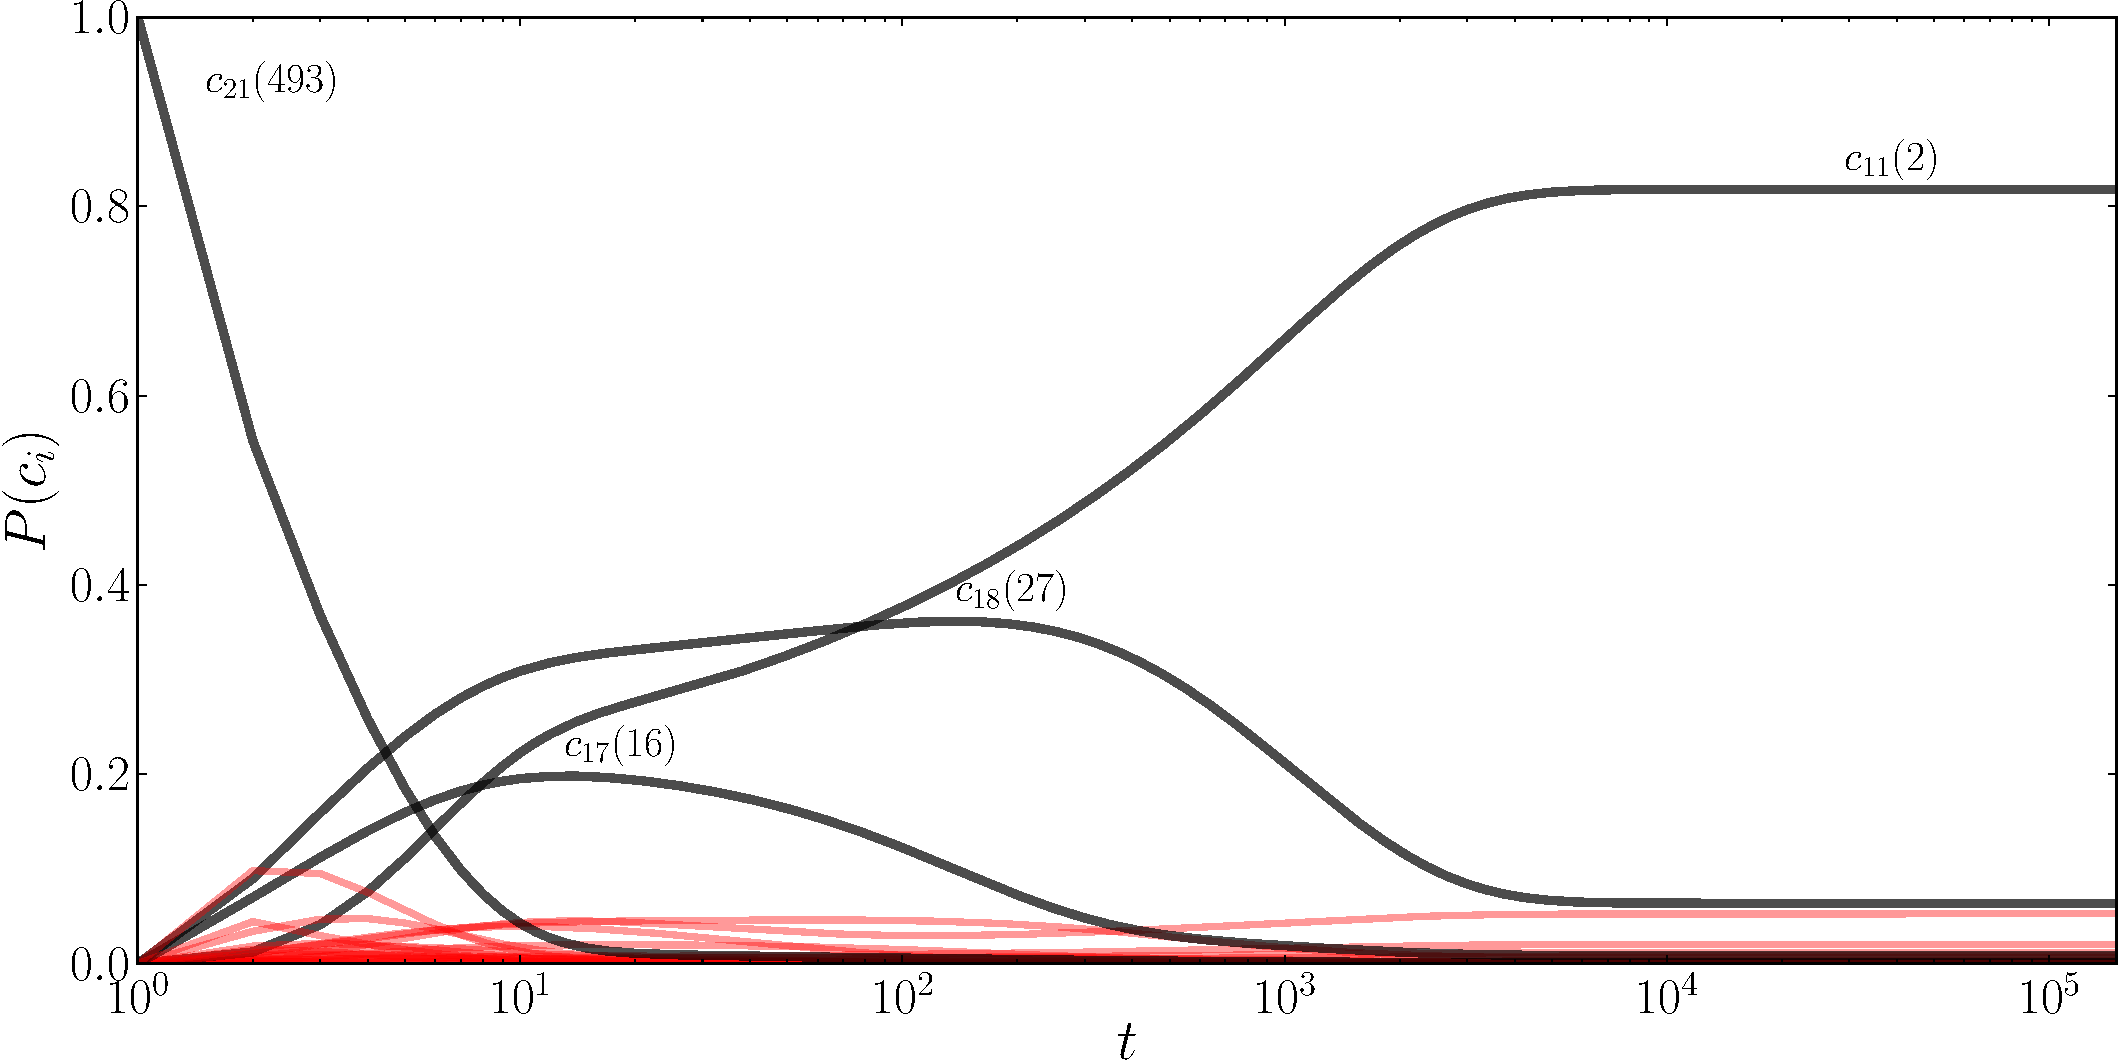
\includegraphics[width=\textwidth]{supplement/beta_cluster_example_2/pictures/kinetics_beta_cluster.pdf}
  \caption{
    Cluster kinetics for the $\beta$-hairpin over a logarithmic time axis. Starting at the completely unfolded state, the motion spans many decades before it folds in the native state. For clarity, the clusters with a significant population are labeled and shown in black. The other clusters are shown in red.
  }
  \label{fig:beta_hairpin_kinetics}
\end{figure}
%

With the interesting clusters identified, we can examine them for any shared property. The microstates are shown at different scales for visual clarity (long, narrow microstates may appear smaller than globular ones). Shown below is the final cluster $c_{11},$ clearly containing native state.
\inlineframebox{\B{Native state cluster} $c_{11}$}{
  \begin{tabular}{ c c }
    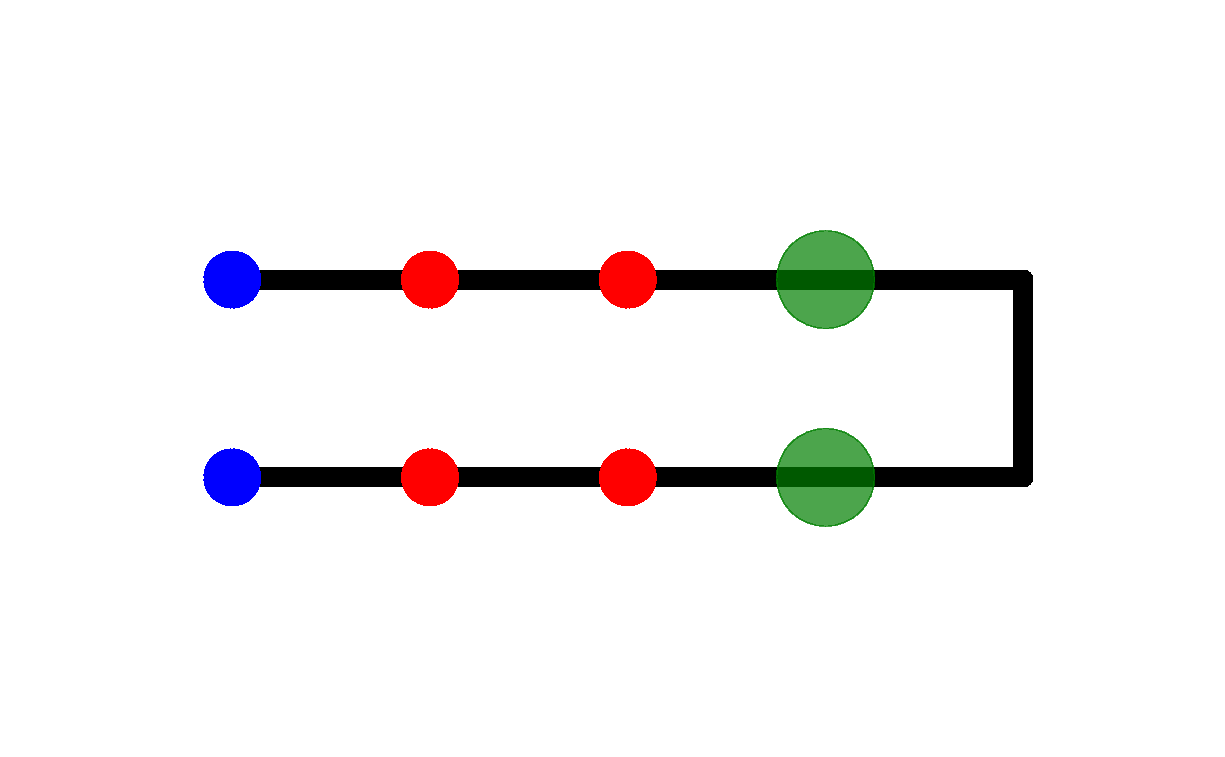
\includegraphics[width=.25\textwidth]{supplement/beta_cluster_example_2/pictures/saved_macrostates/state_cluster_shapes_0.png} 
    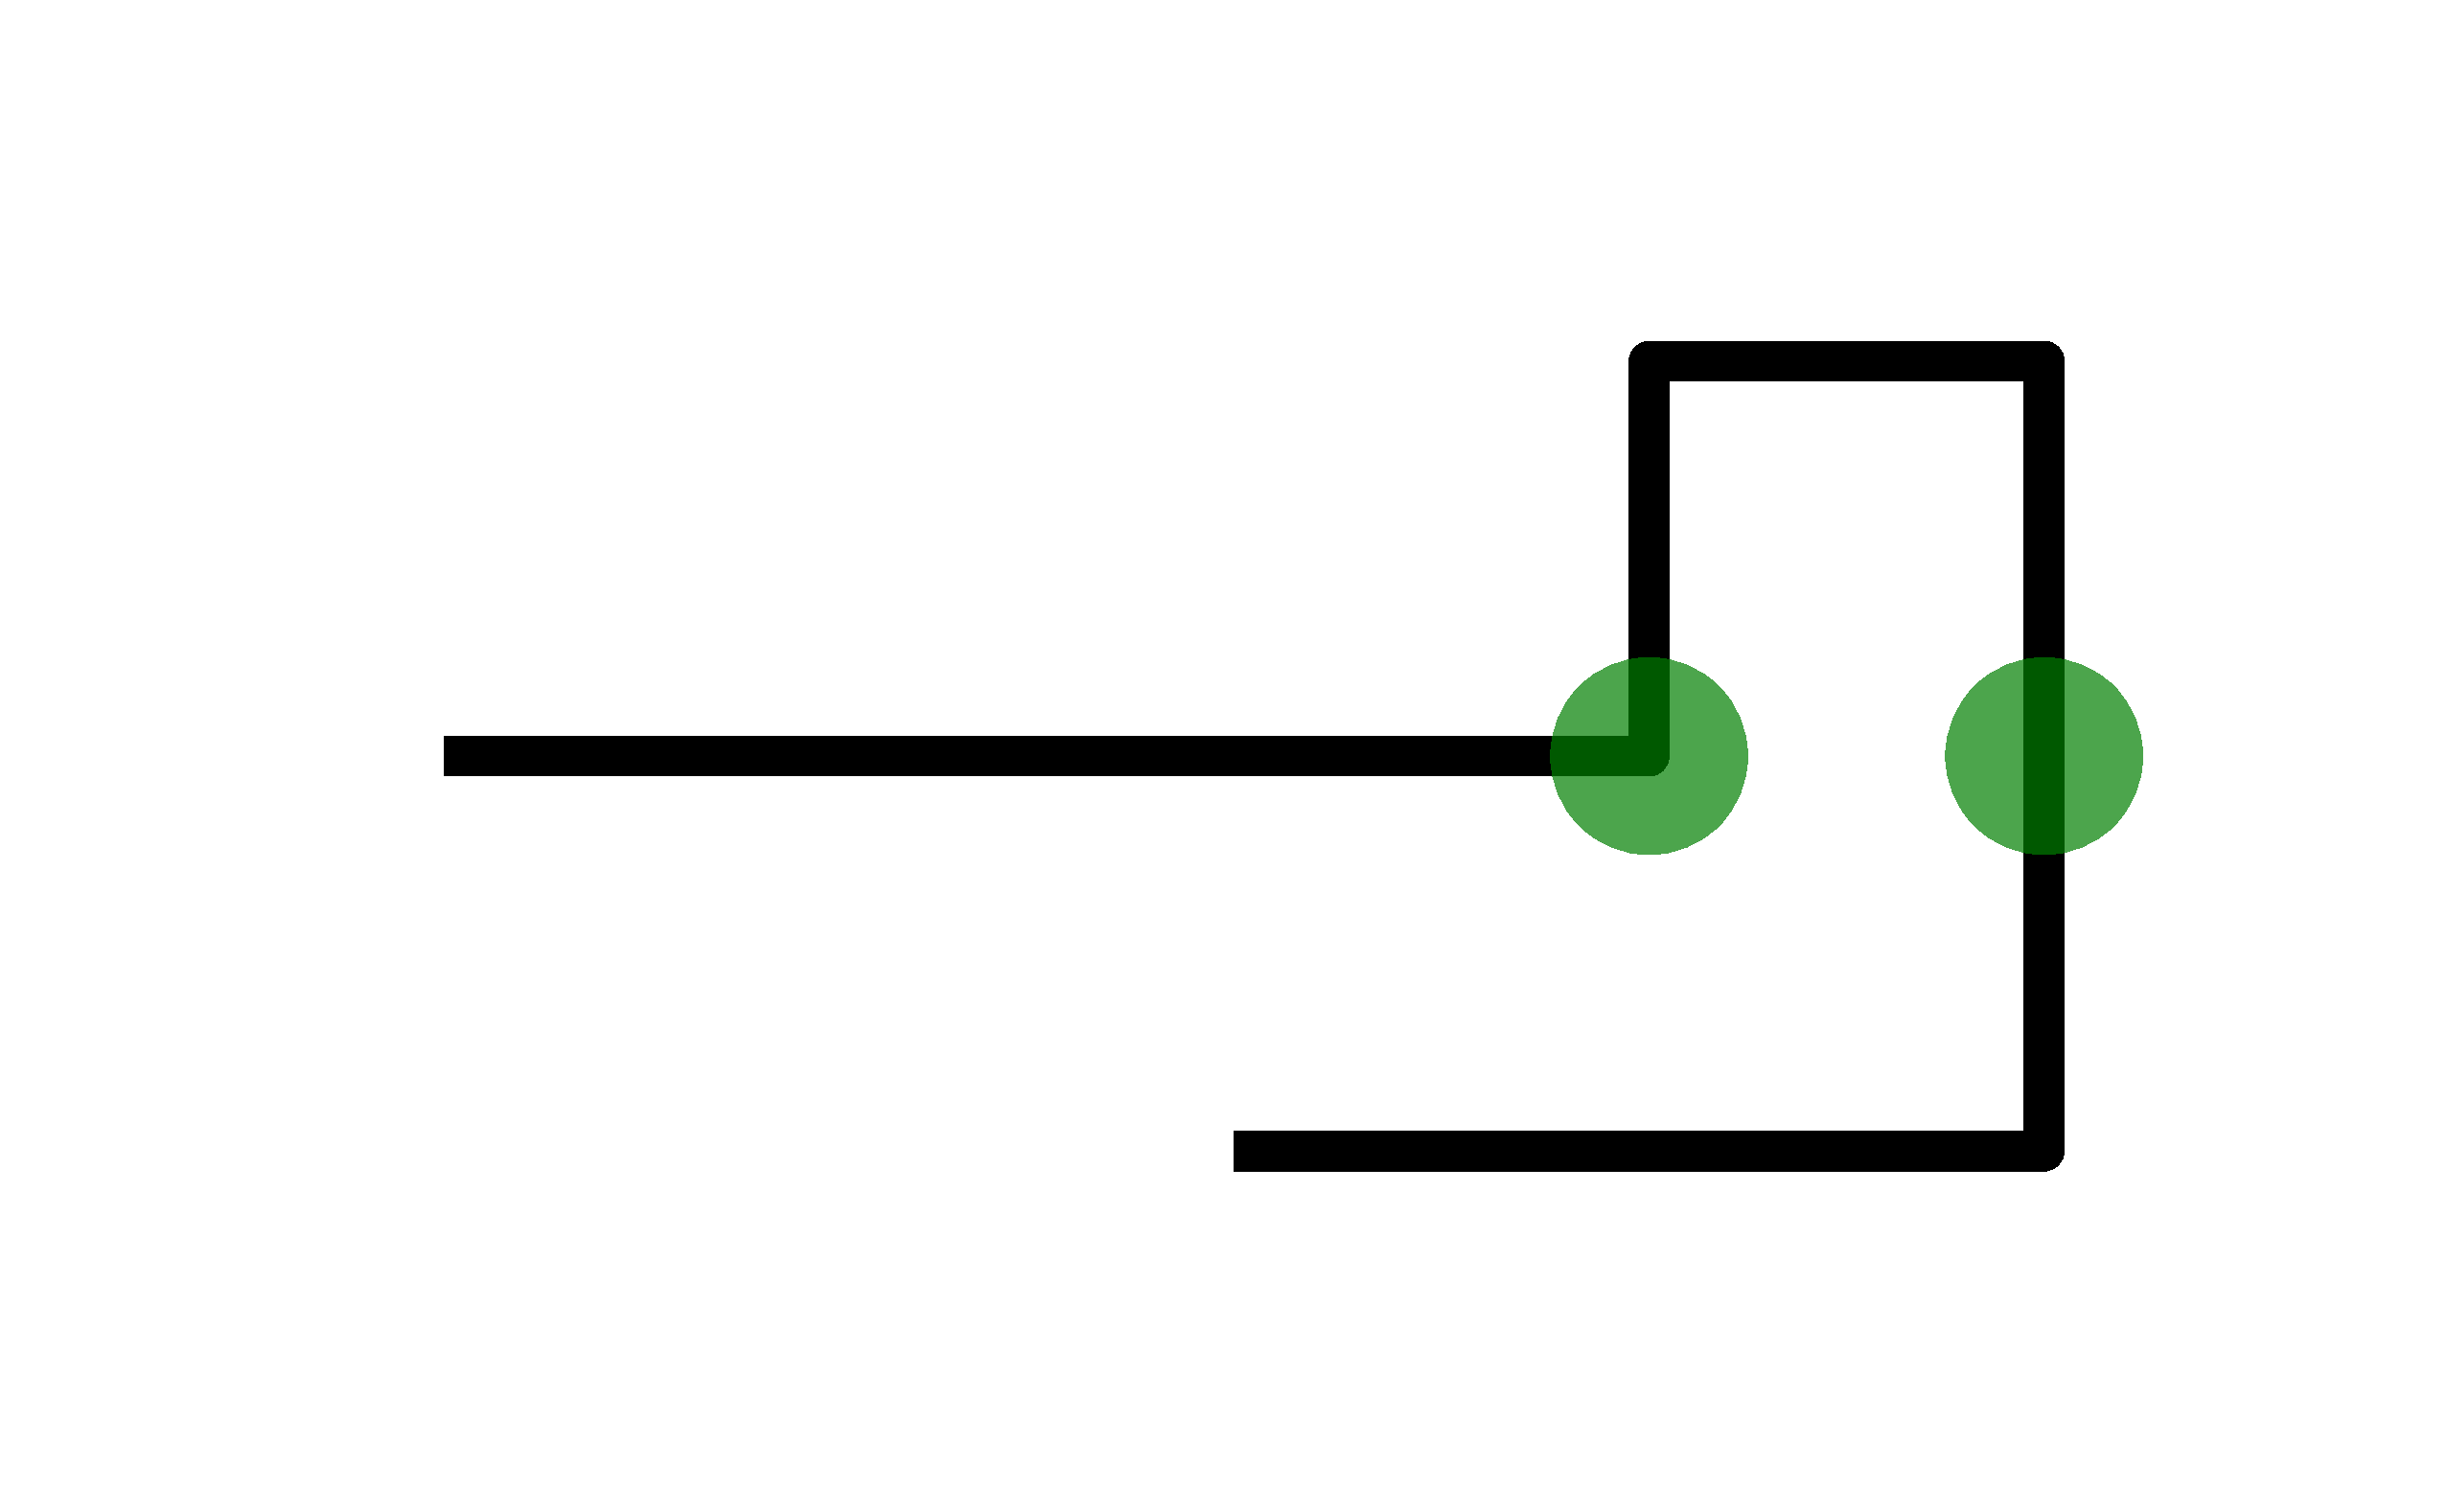
\includegraphics[width=.25\textwidth]{supplement/beta_cluster_example_2/pictures/11/state_cluster_shapes_1.pdf} 
  \end{tabular}
}
The presence of an additional microstate is not unexpected. As we saw before in the FLW walk, local minima are often associated with the same cluster.
All of the microstates in the other two intermediate clusters have one particular thing in common, the formation of the salt bridge. Listed below are six representative conformations in each of the two intermediate clusters
%
\inlineframebox{\B{Intermediate Cluster} $c_{17}$} {
  \begin{tabular}{ c c c }
    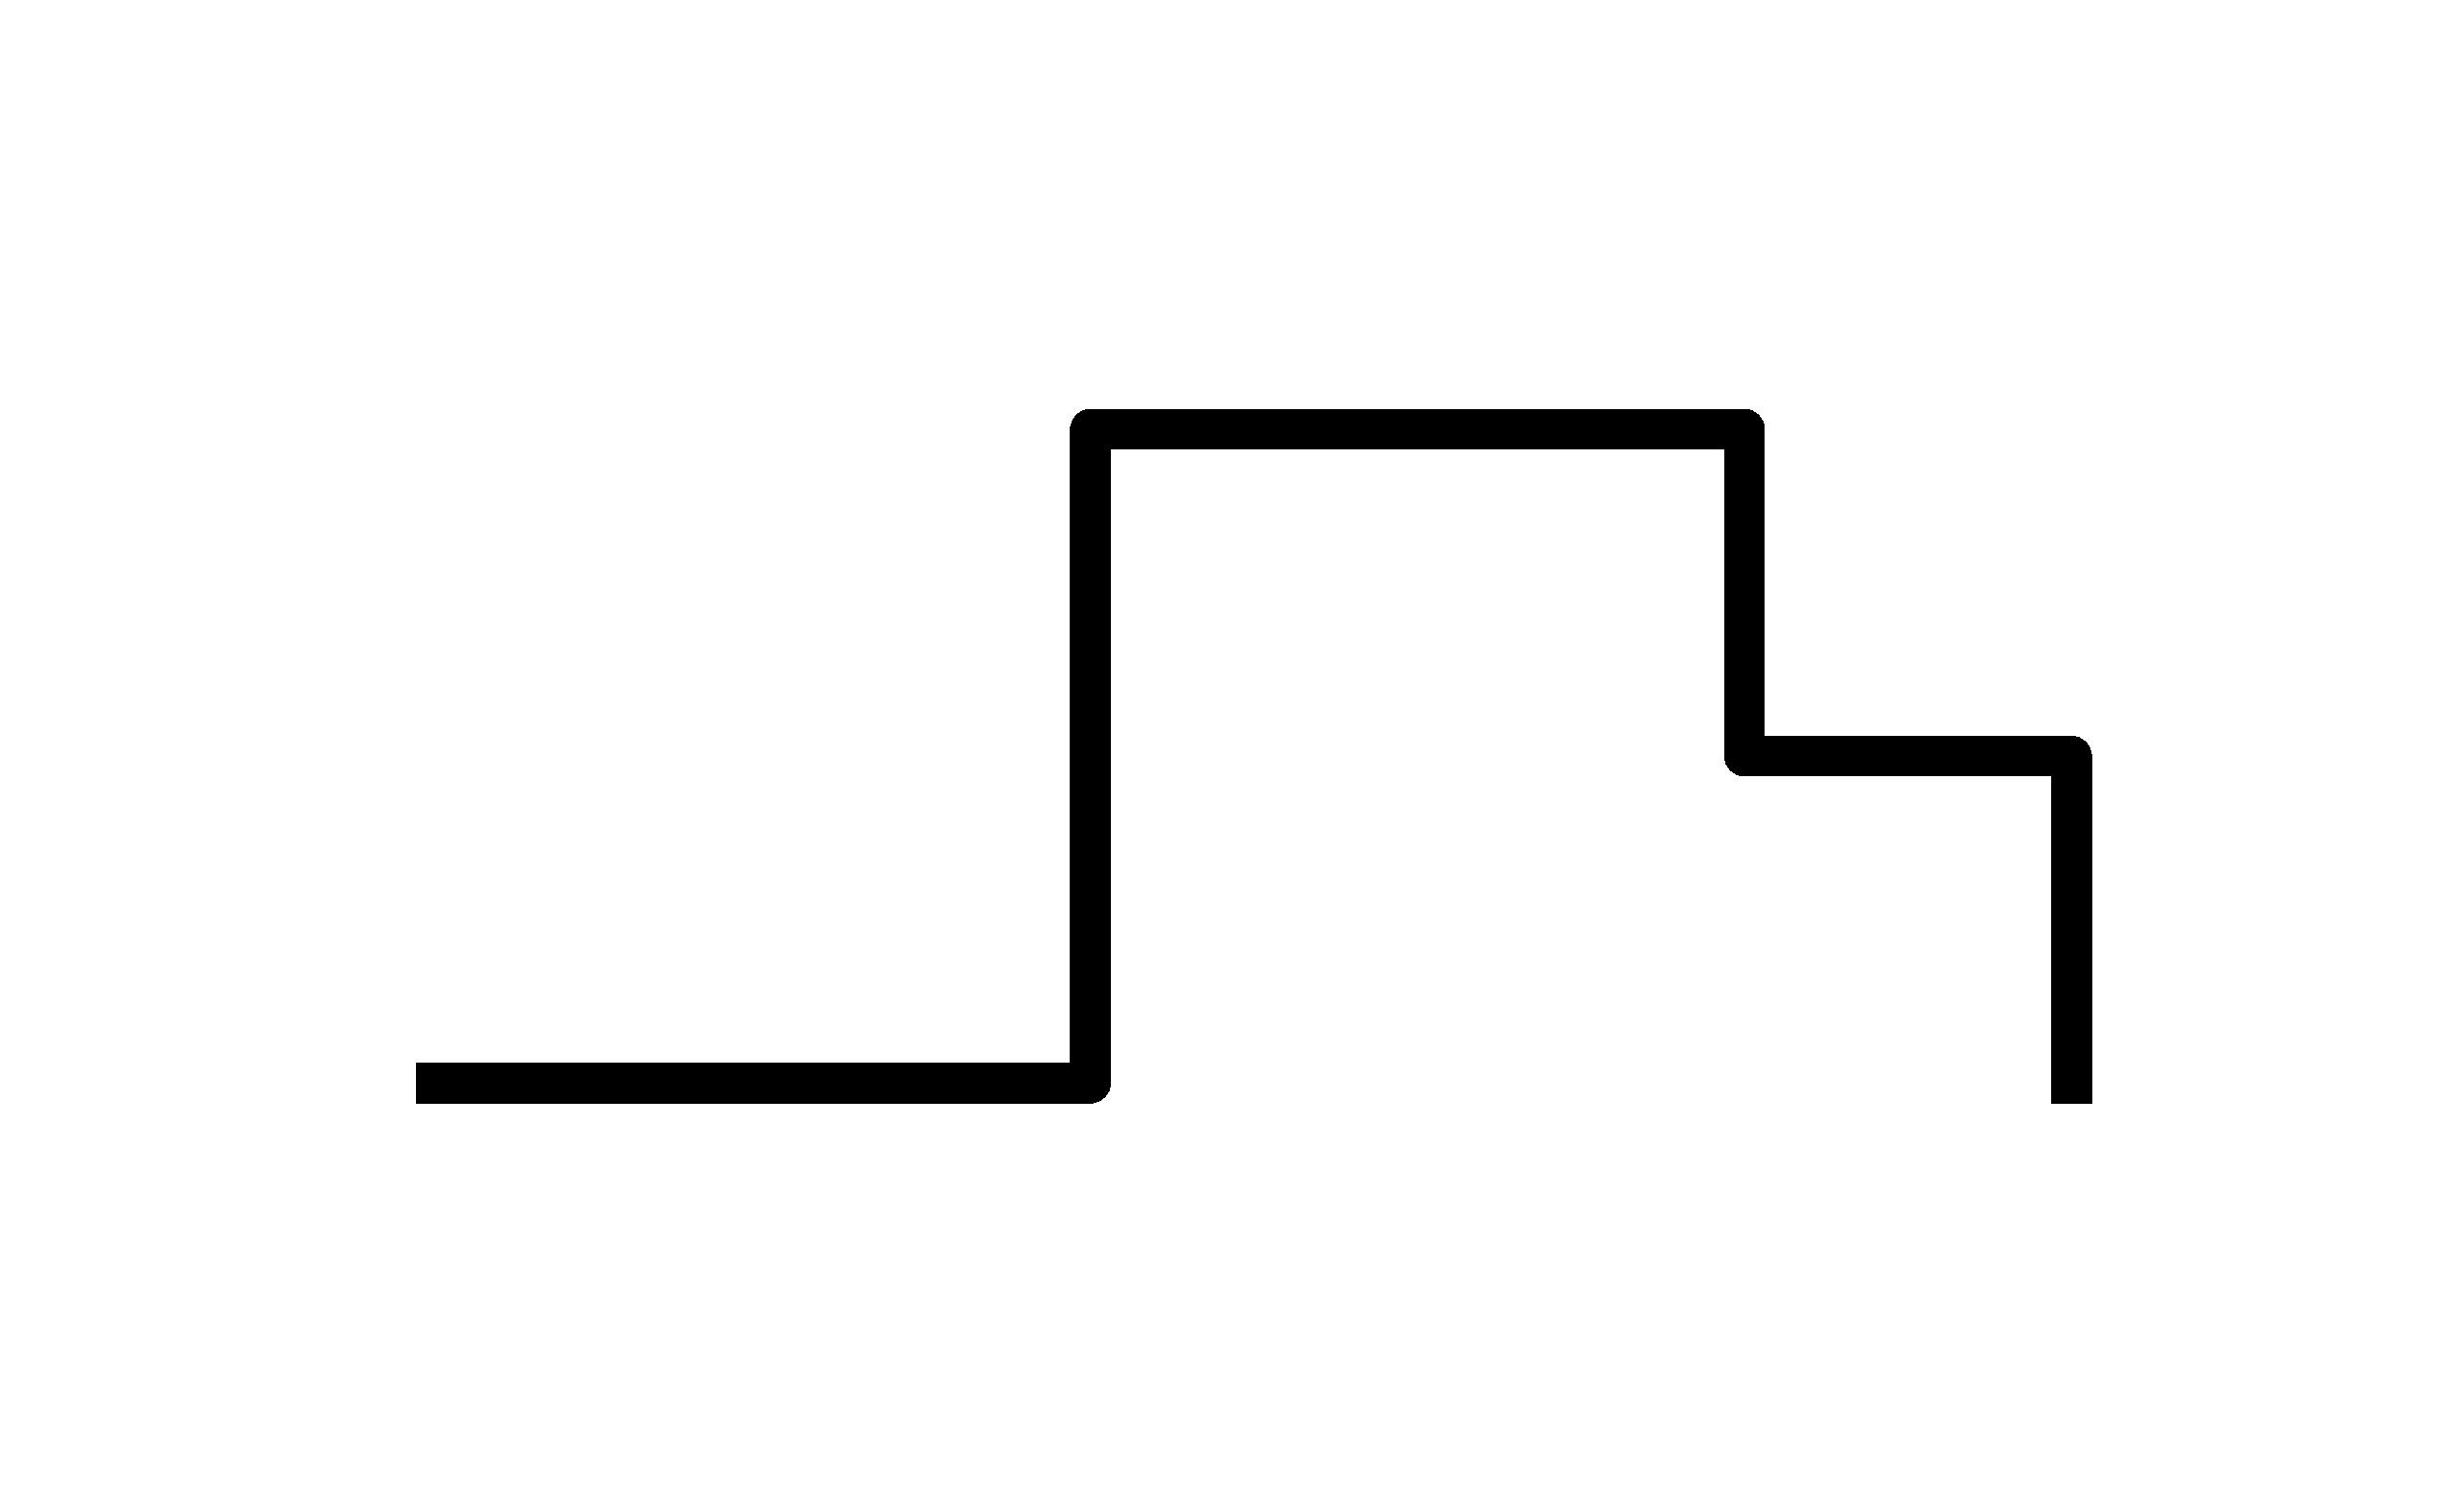
\includegraphics[width=.252\linewidth]{supplement/beta_cluster_example_2/pictures/17/state_cluster_shapes_0.pdf} &
    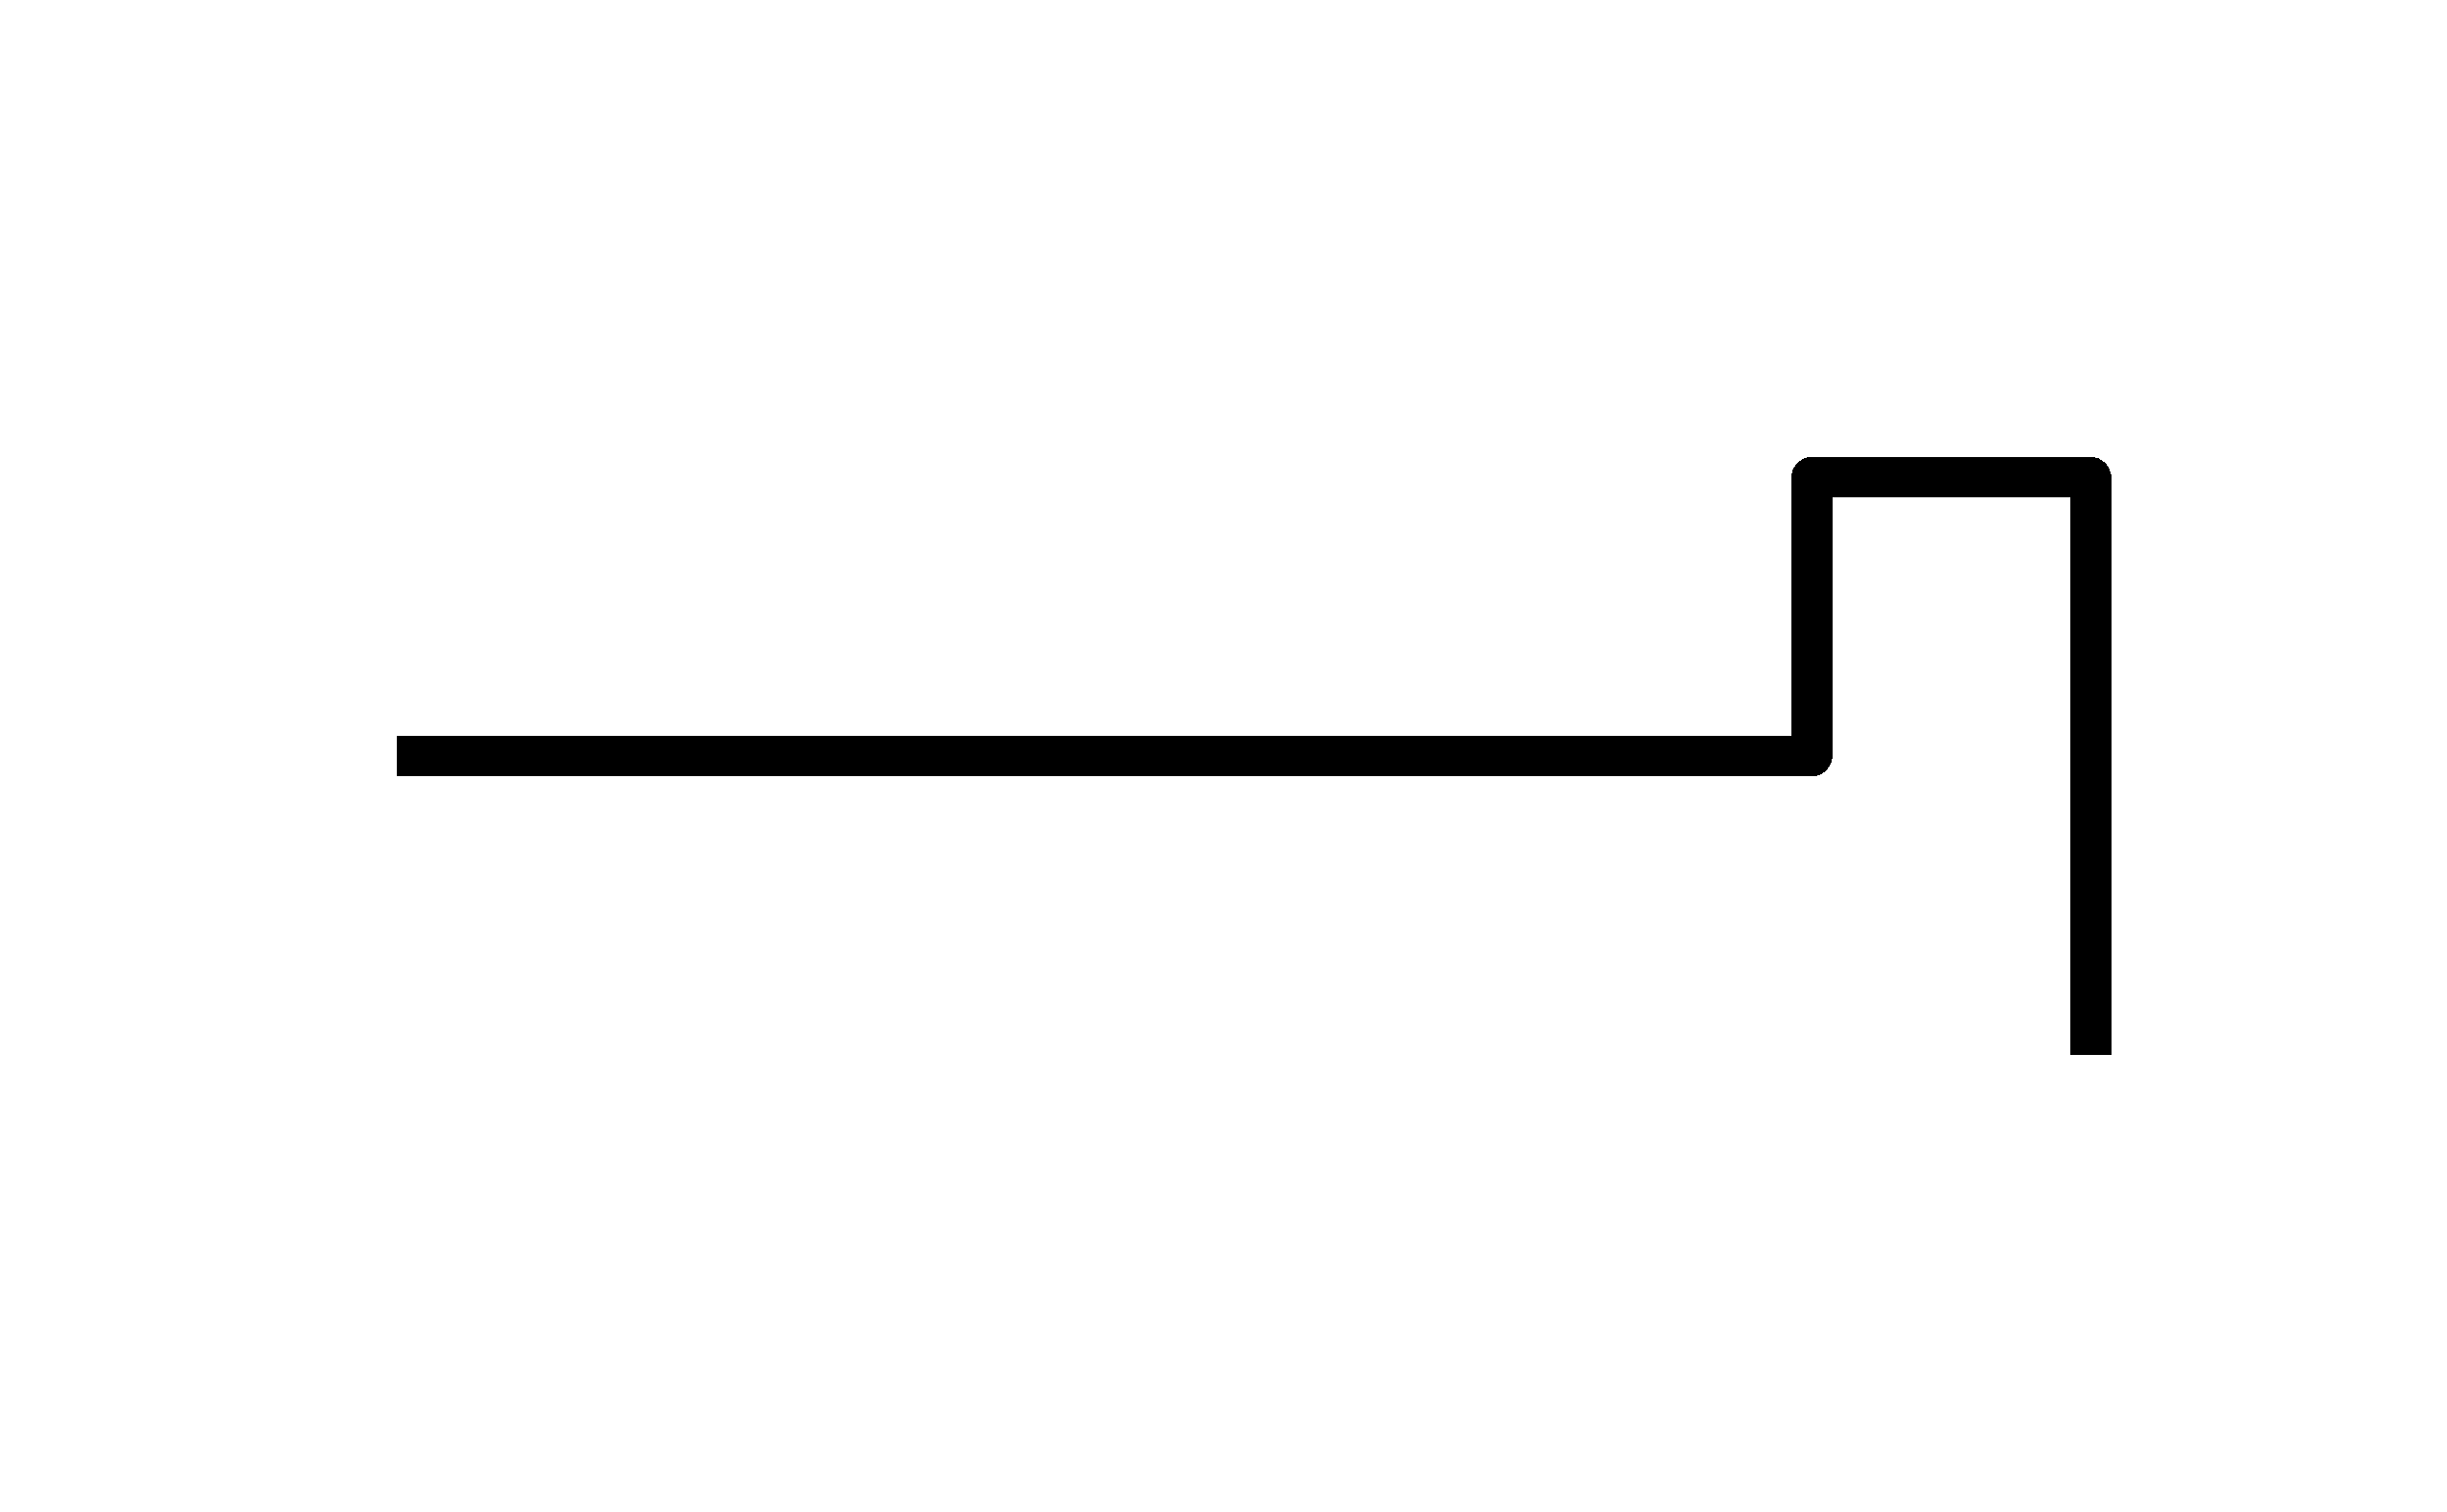
\includegraphics[width=.252\linewidth]{supplement/beta_cluster_example_2/pictures/17/state_cluster_shapes_1.pdf} & 
    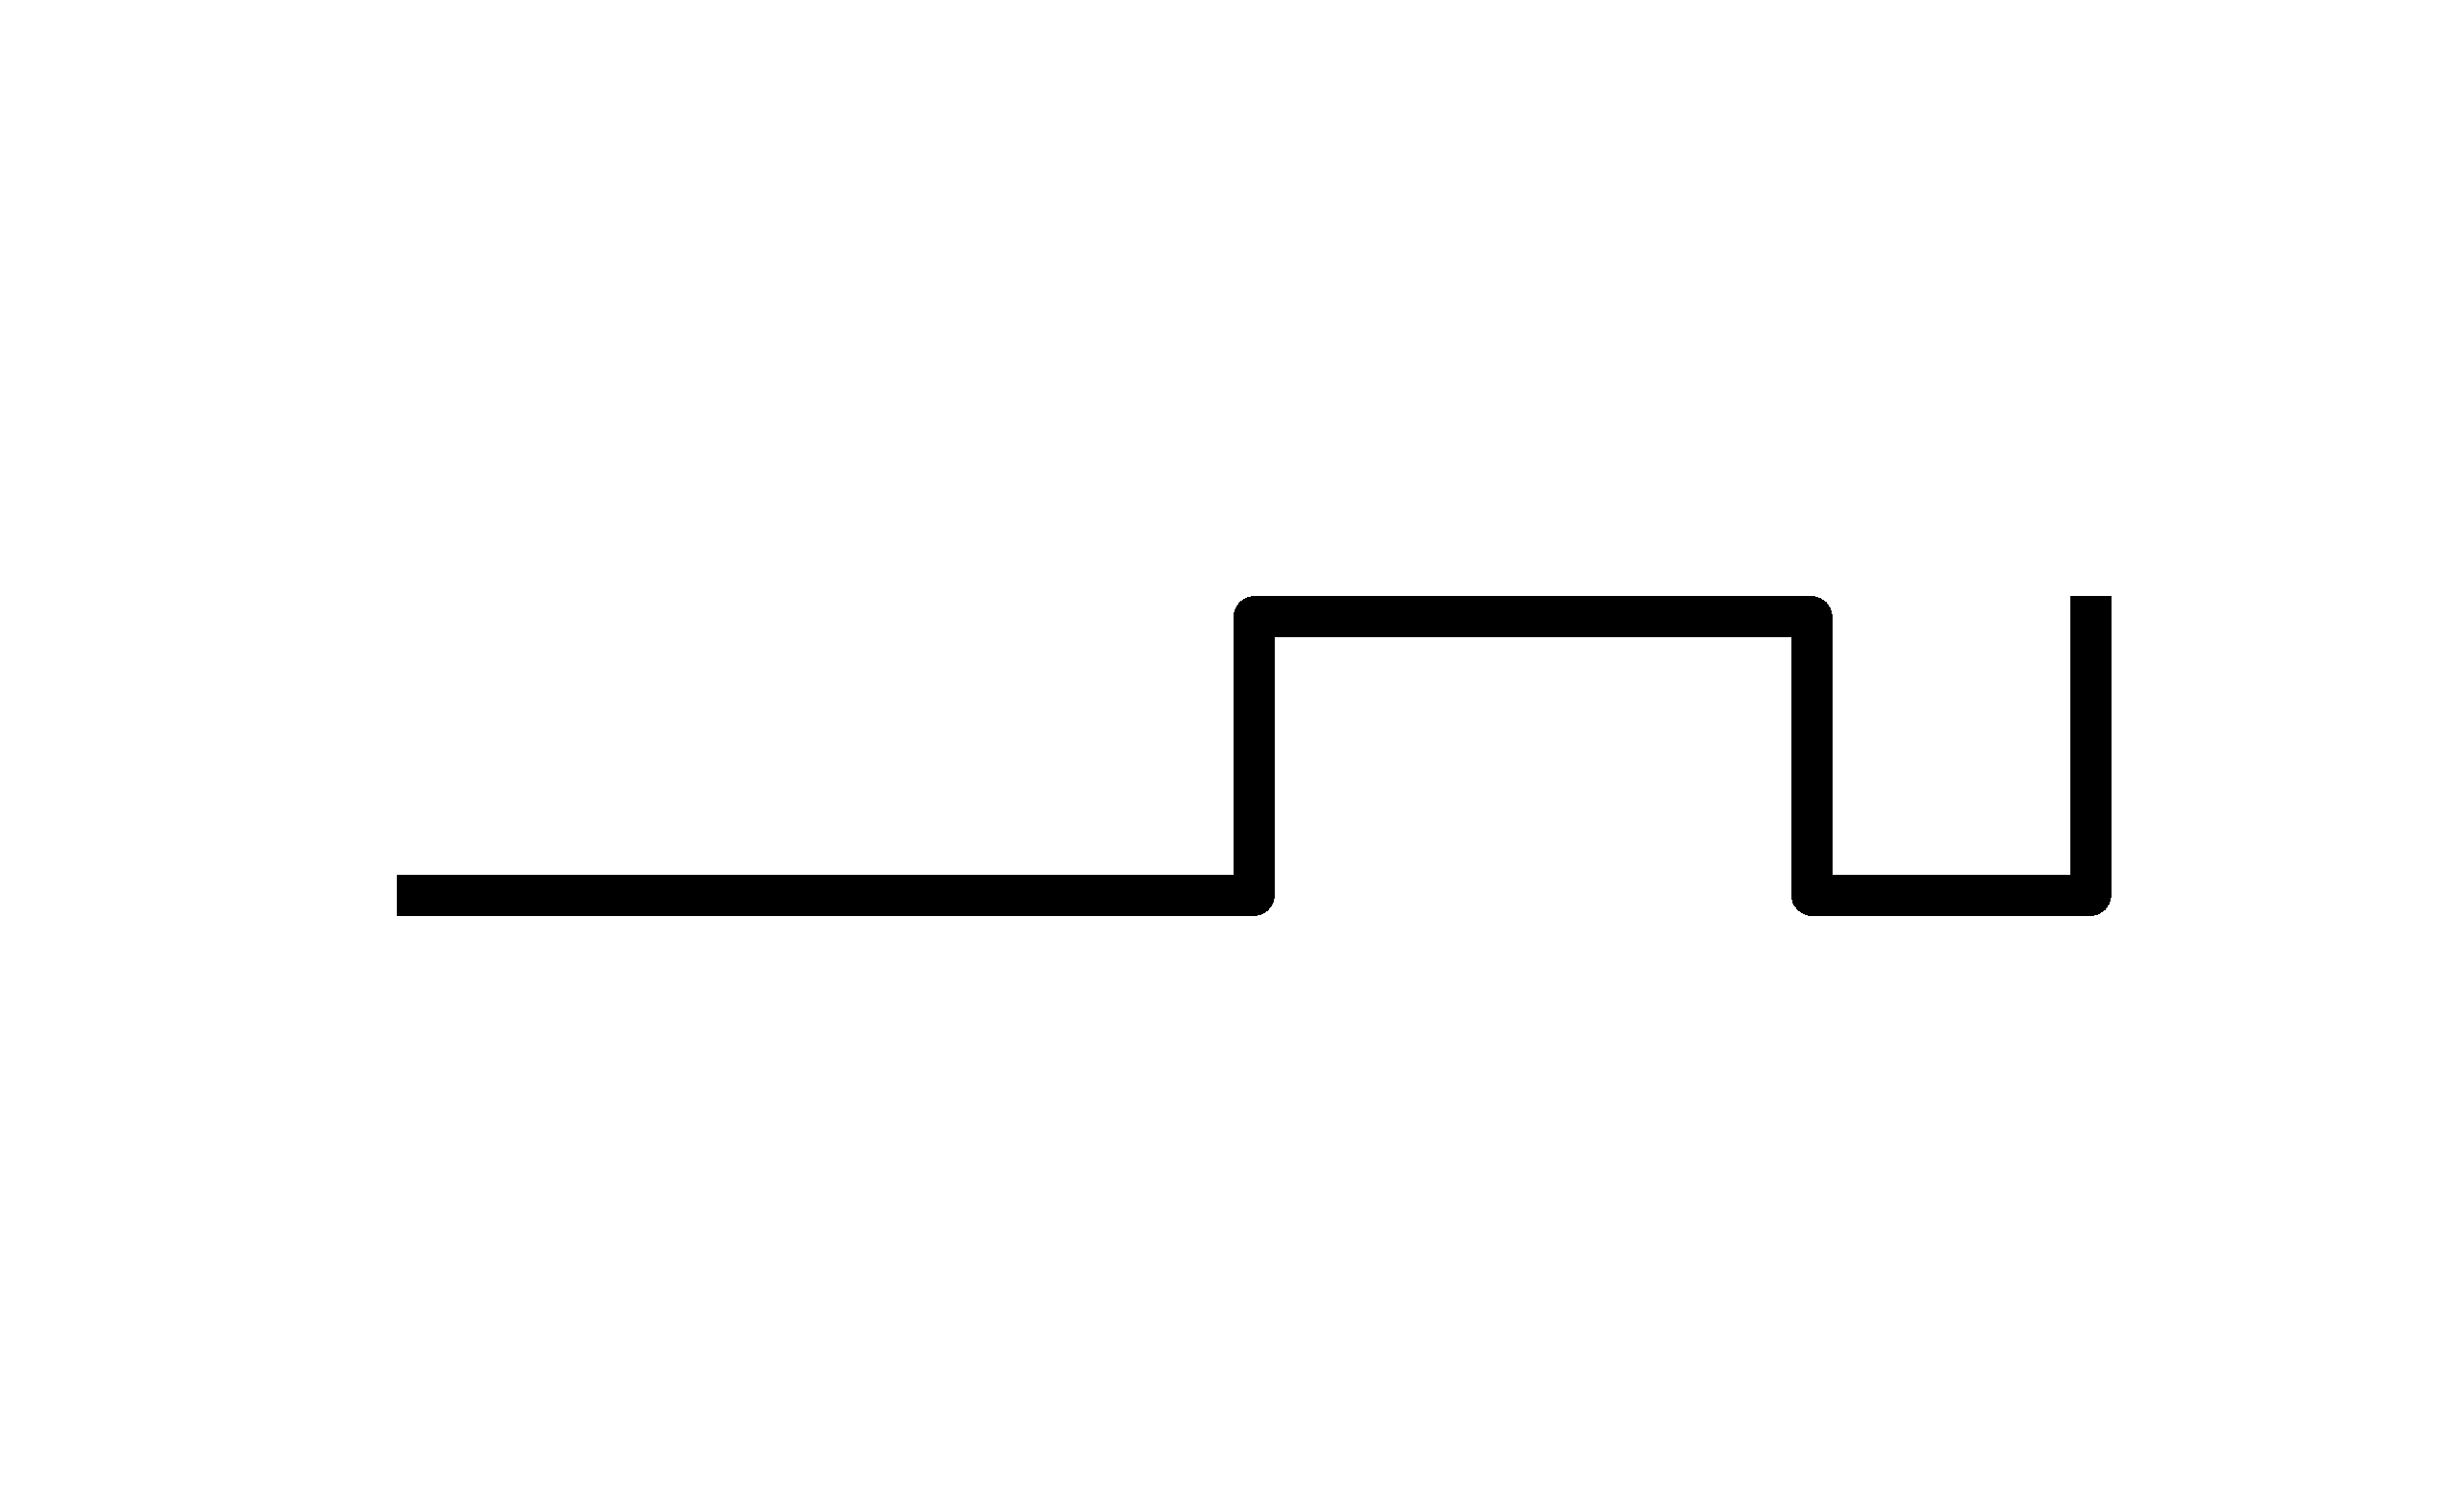
\includegraphics[width=.252\linewidth]{supplement/beta_cluster_example_2/pictures/17/state_cluster_shapes_2.pdf} \\
    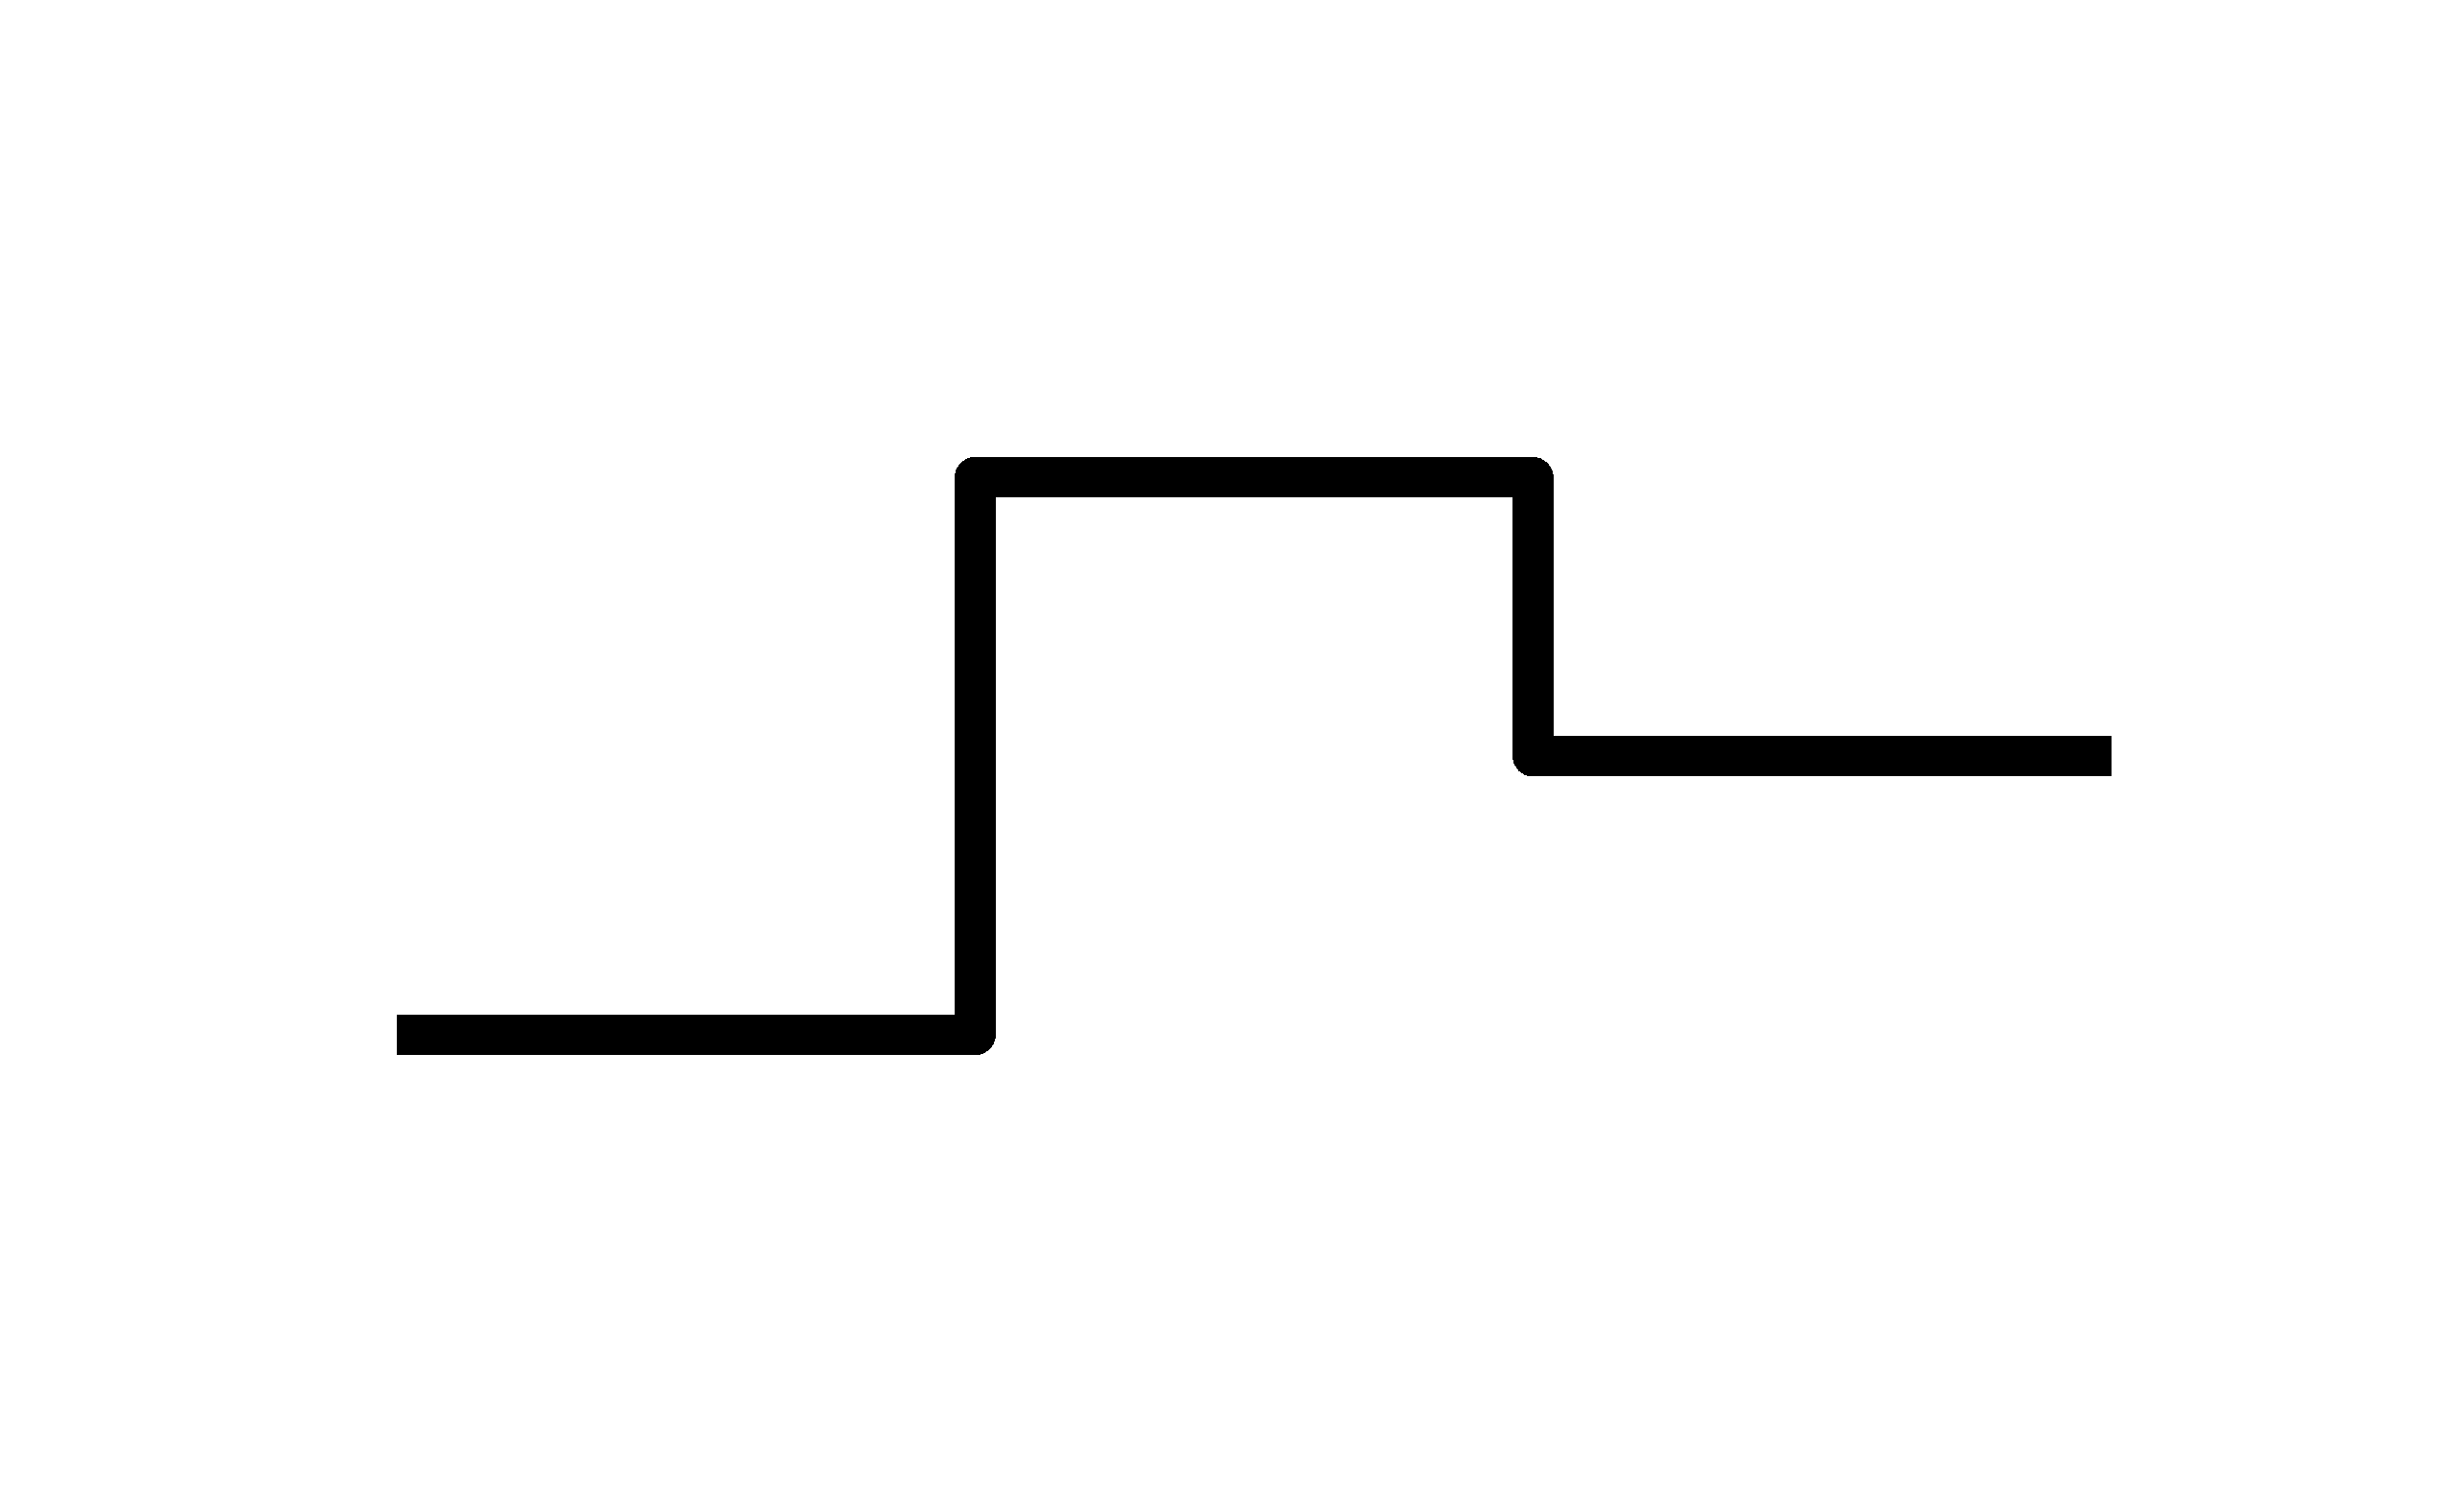
\includegraphics[width=.252\linewidth]{supplement/beta_cluster_example_2/pictures/17/state_cluster_shapes_3.pdf} &
    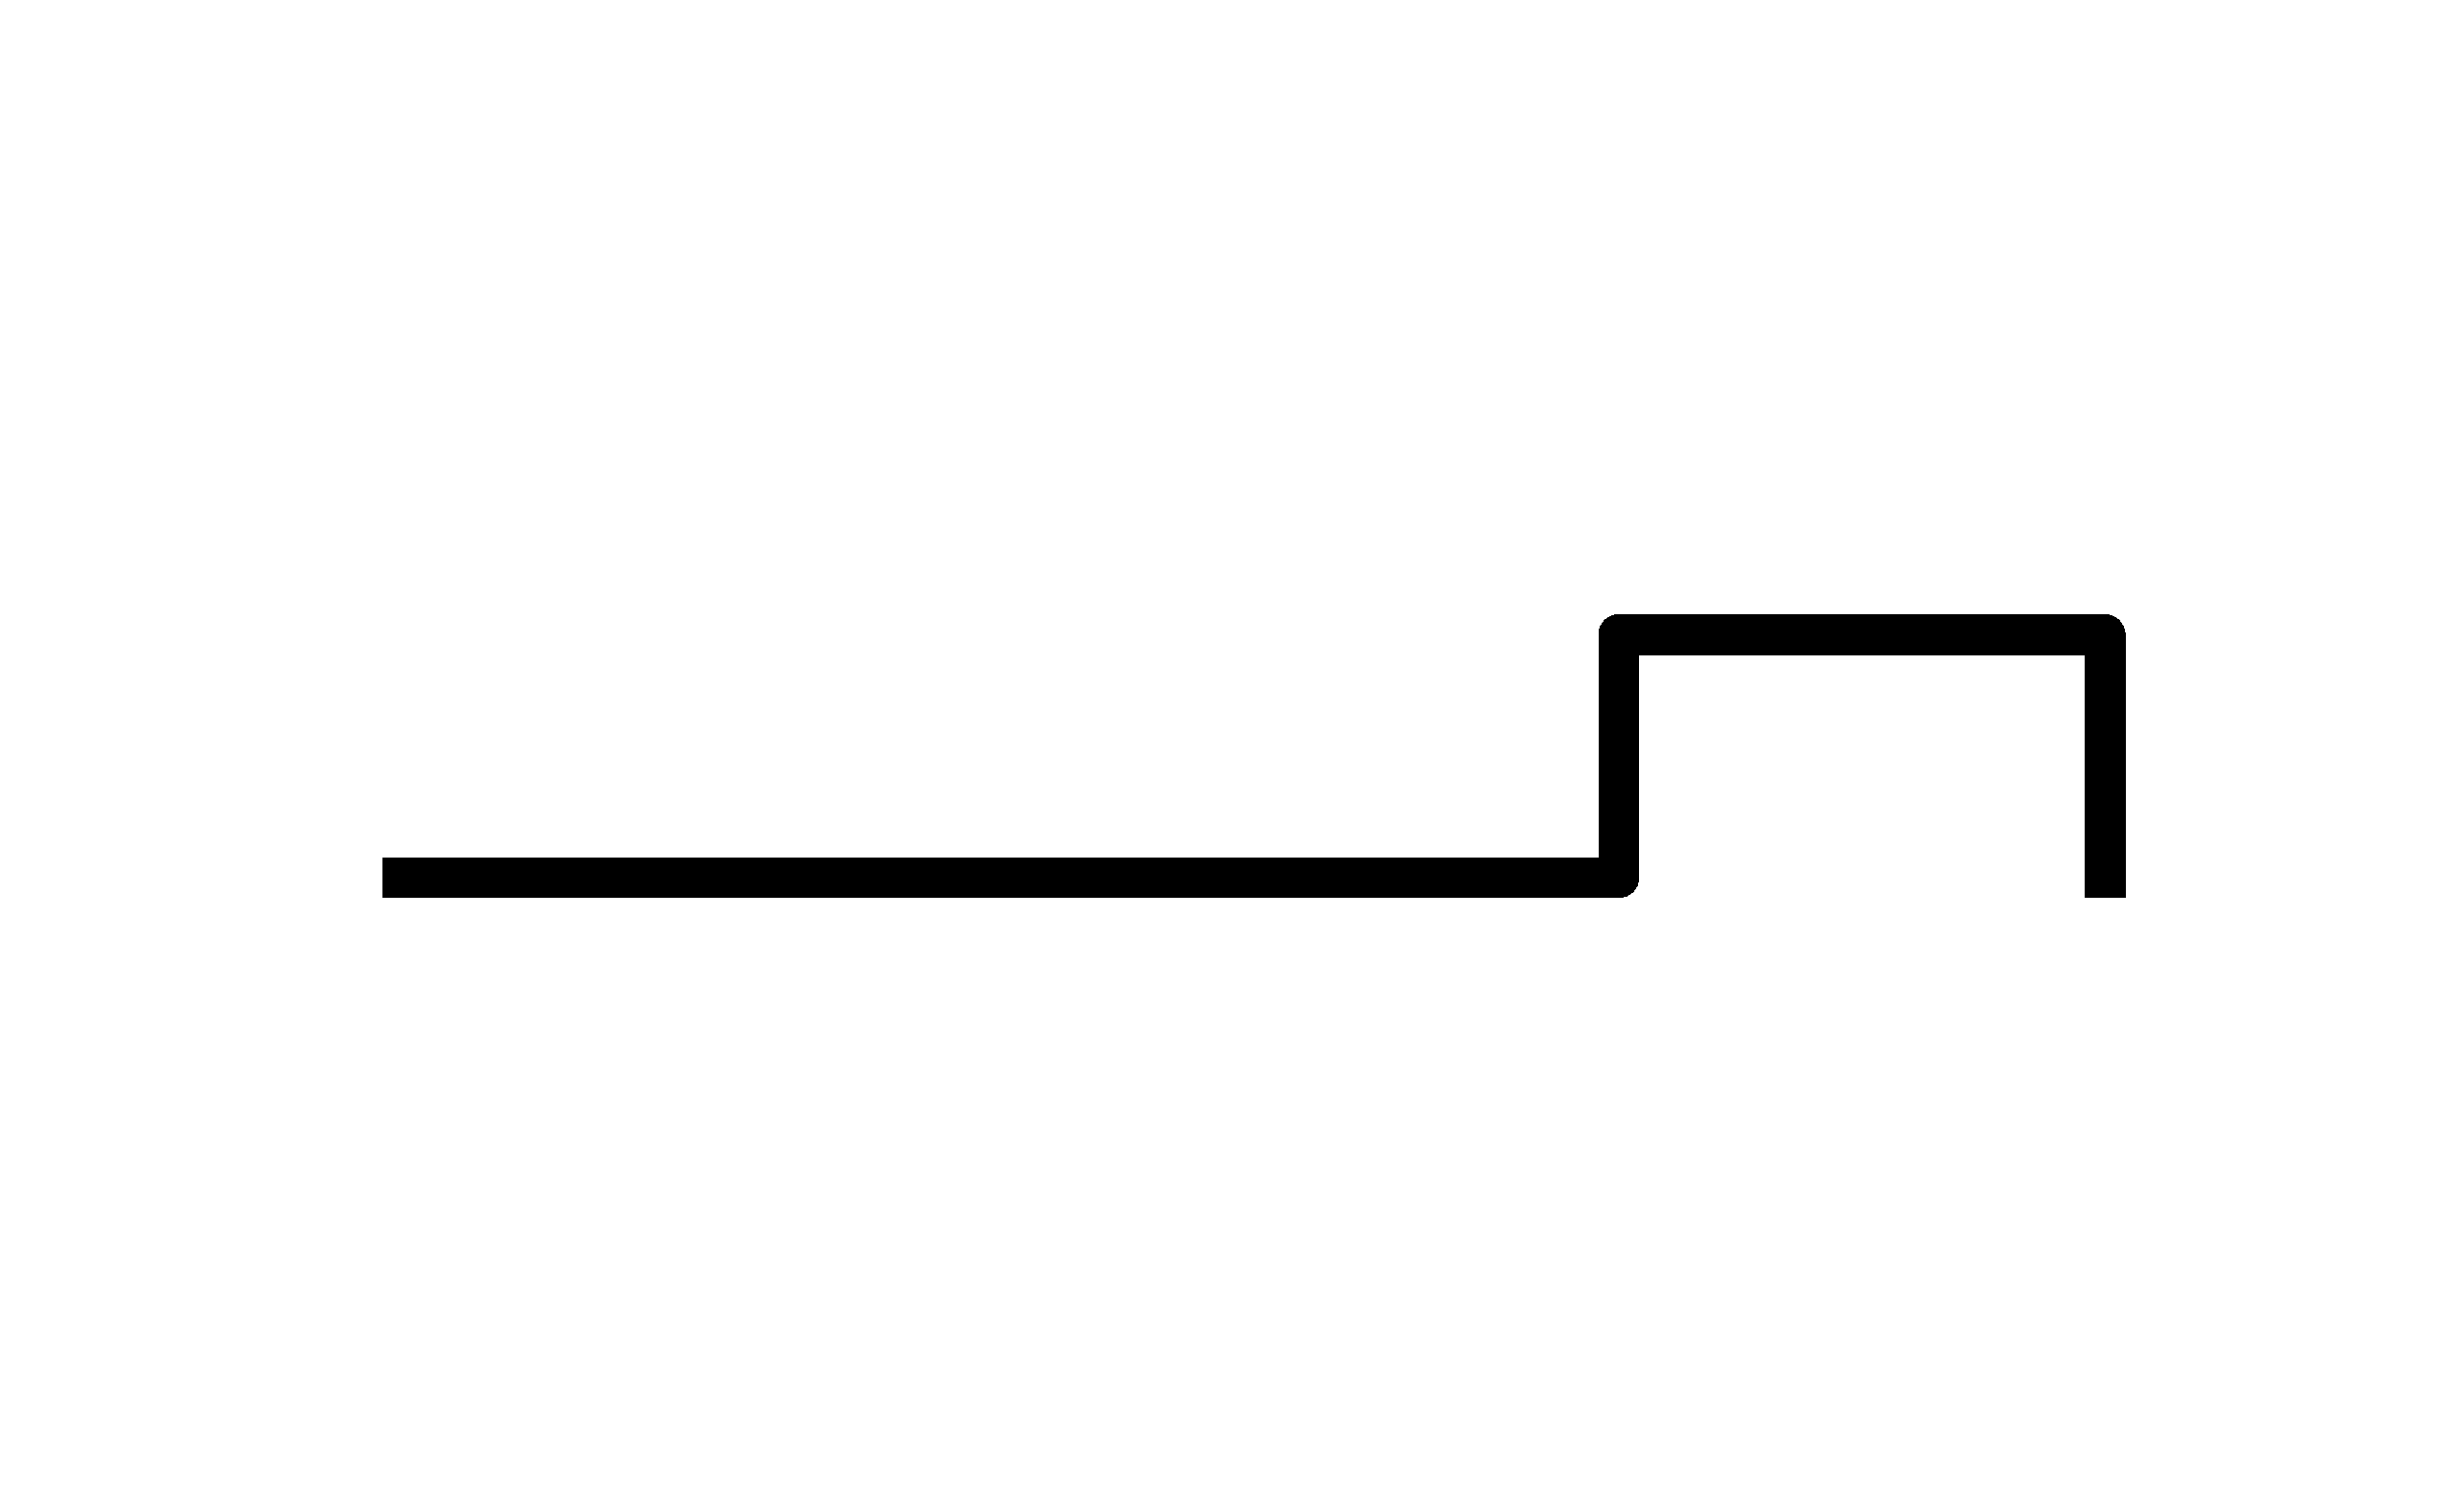
\includegraphics[width=.252\linewidth]{supplement/beta_cluster_example_2/pictures/17/state_cluster_shapes_4.pdf} &
    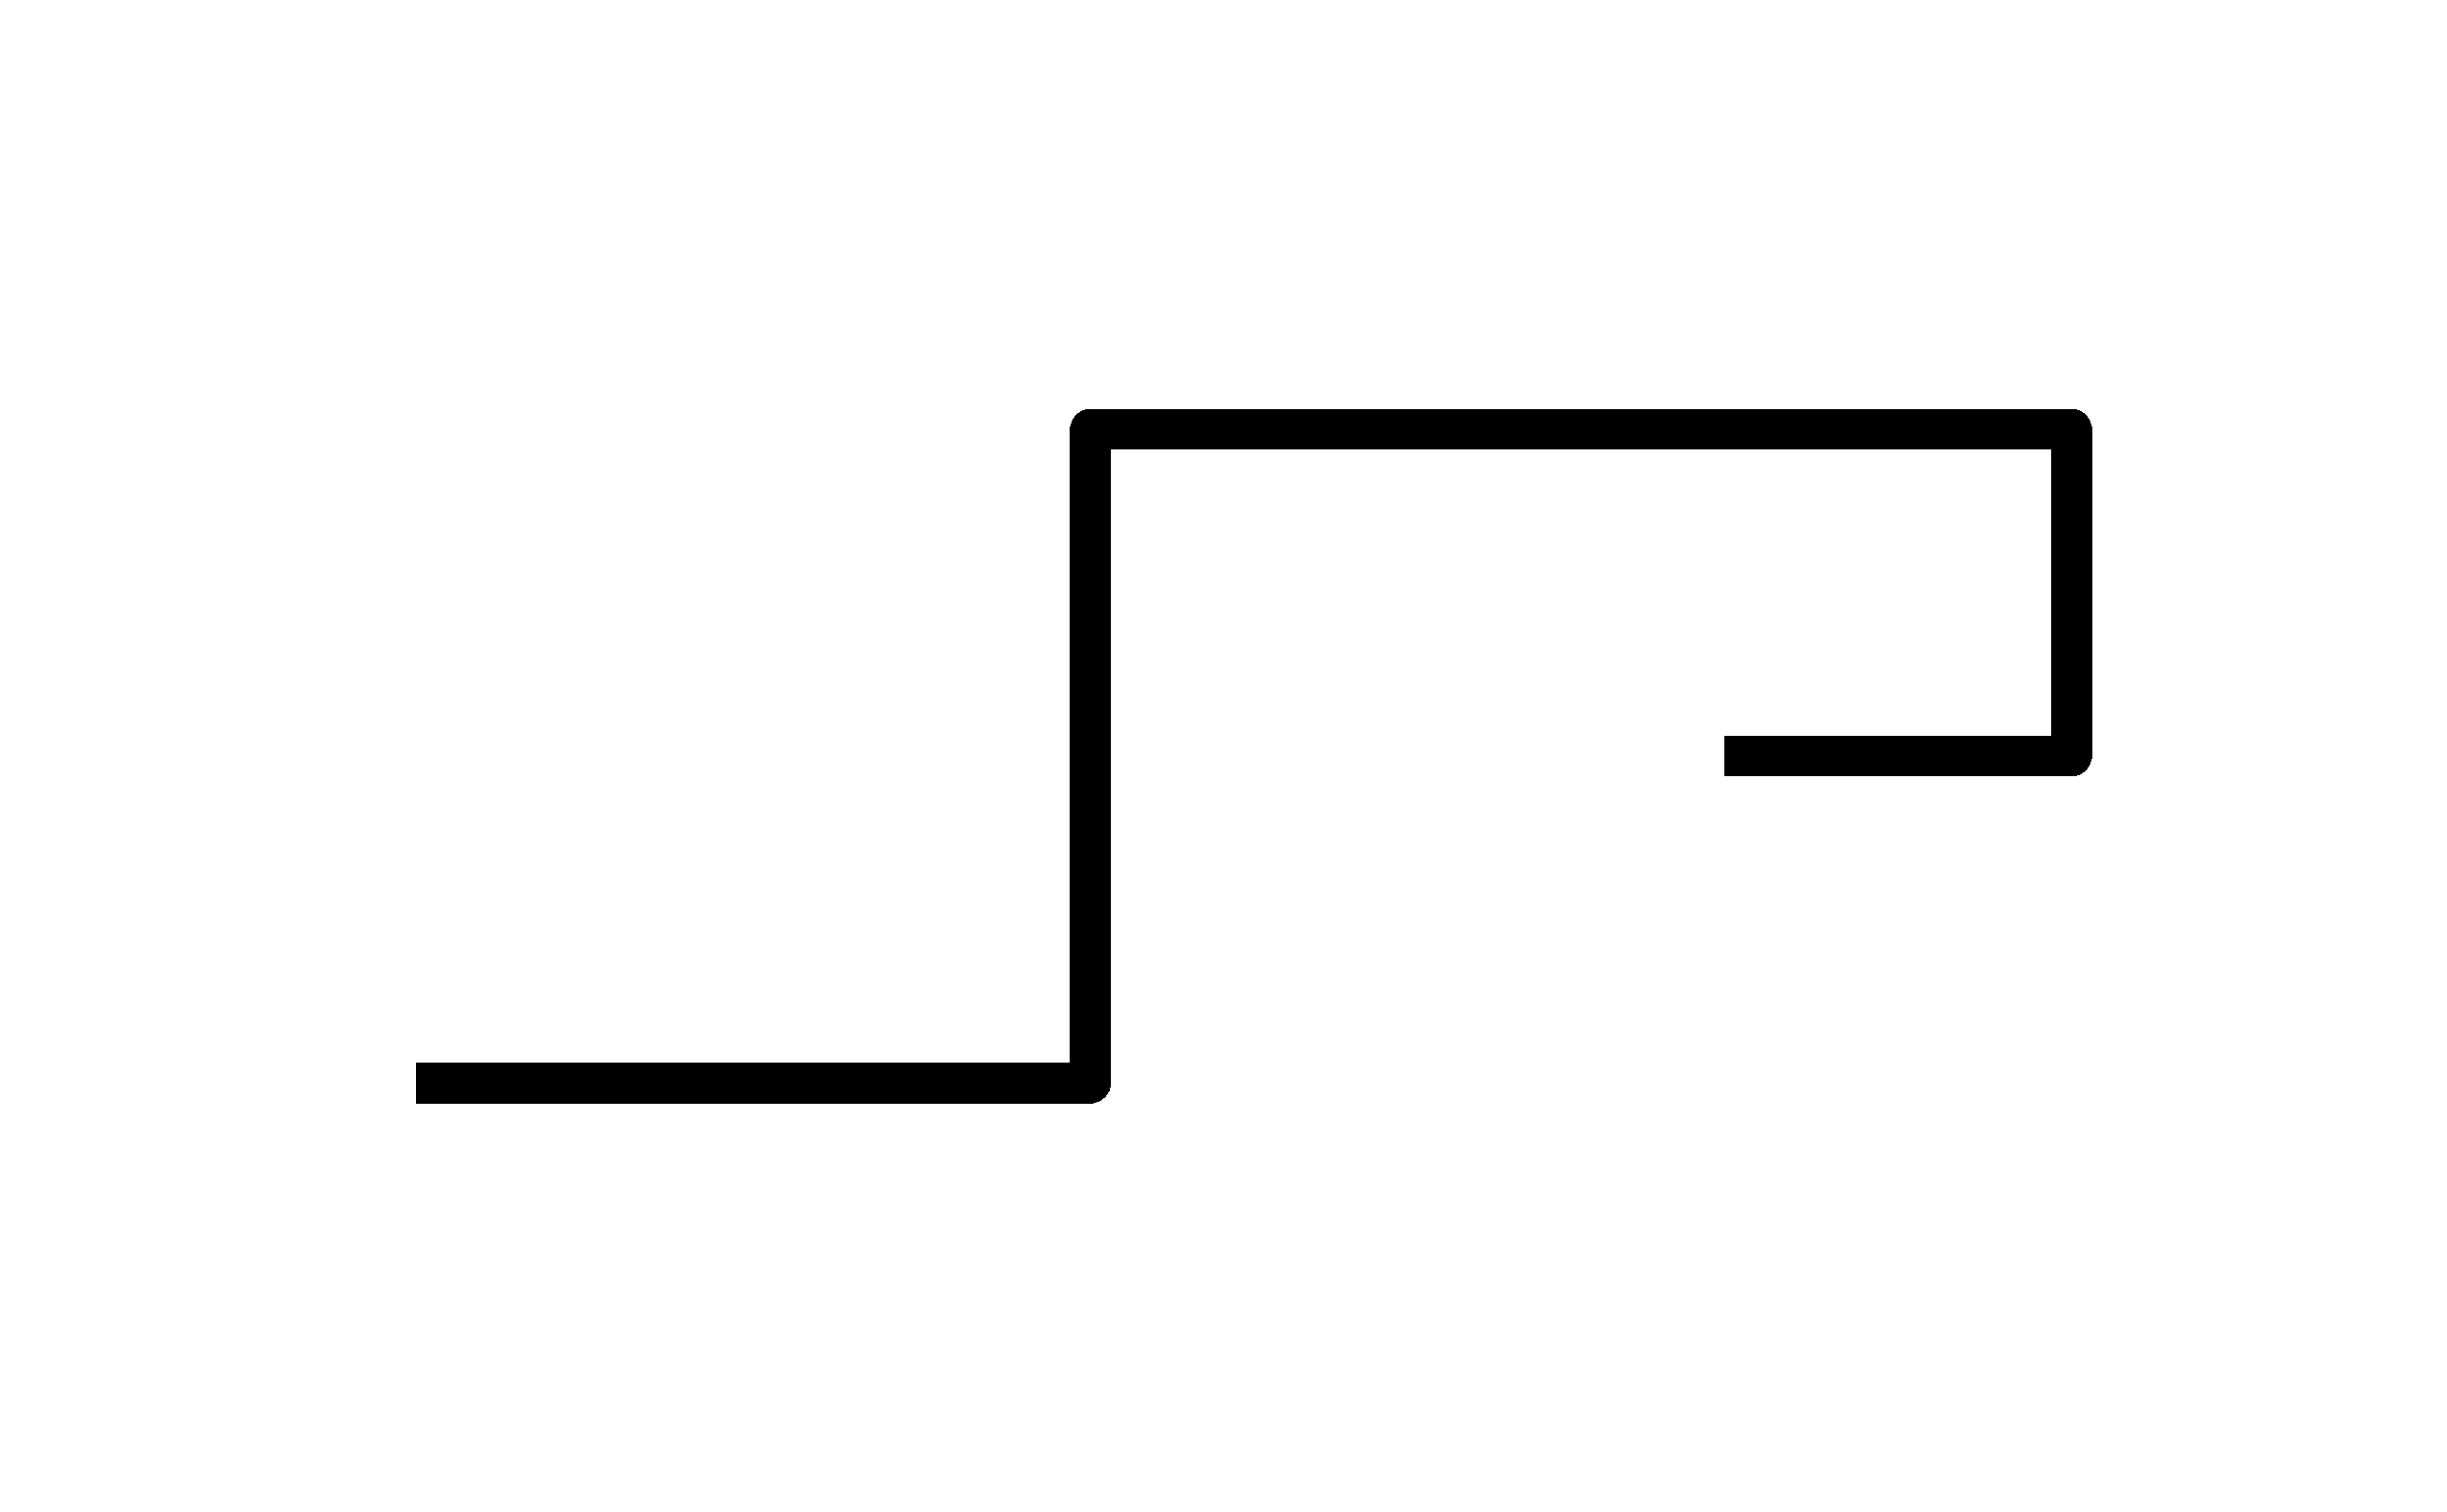
\includegraphics[width=.252\linewidth]{supplement/beta_cluster_example_2/pictures/17/state_cluster_shapes_5.pdf} 
  \end{tabular}
}
%
\inlineframebox{\B{Intermediate Cluster} $c_{18}$} {
  \begin{tabular}{ c c c }
    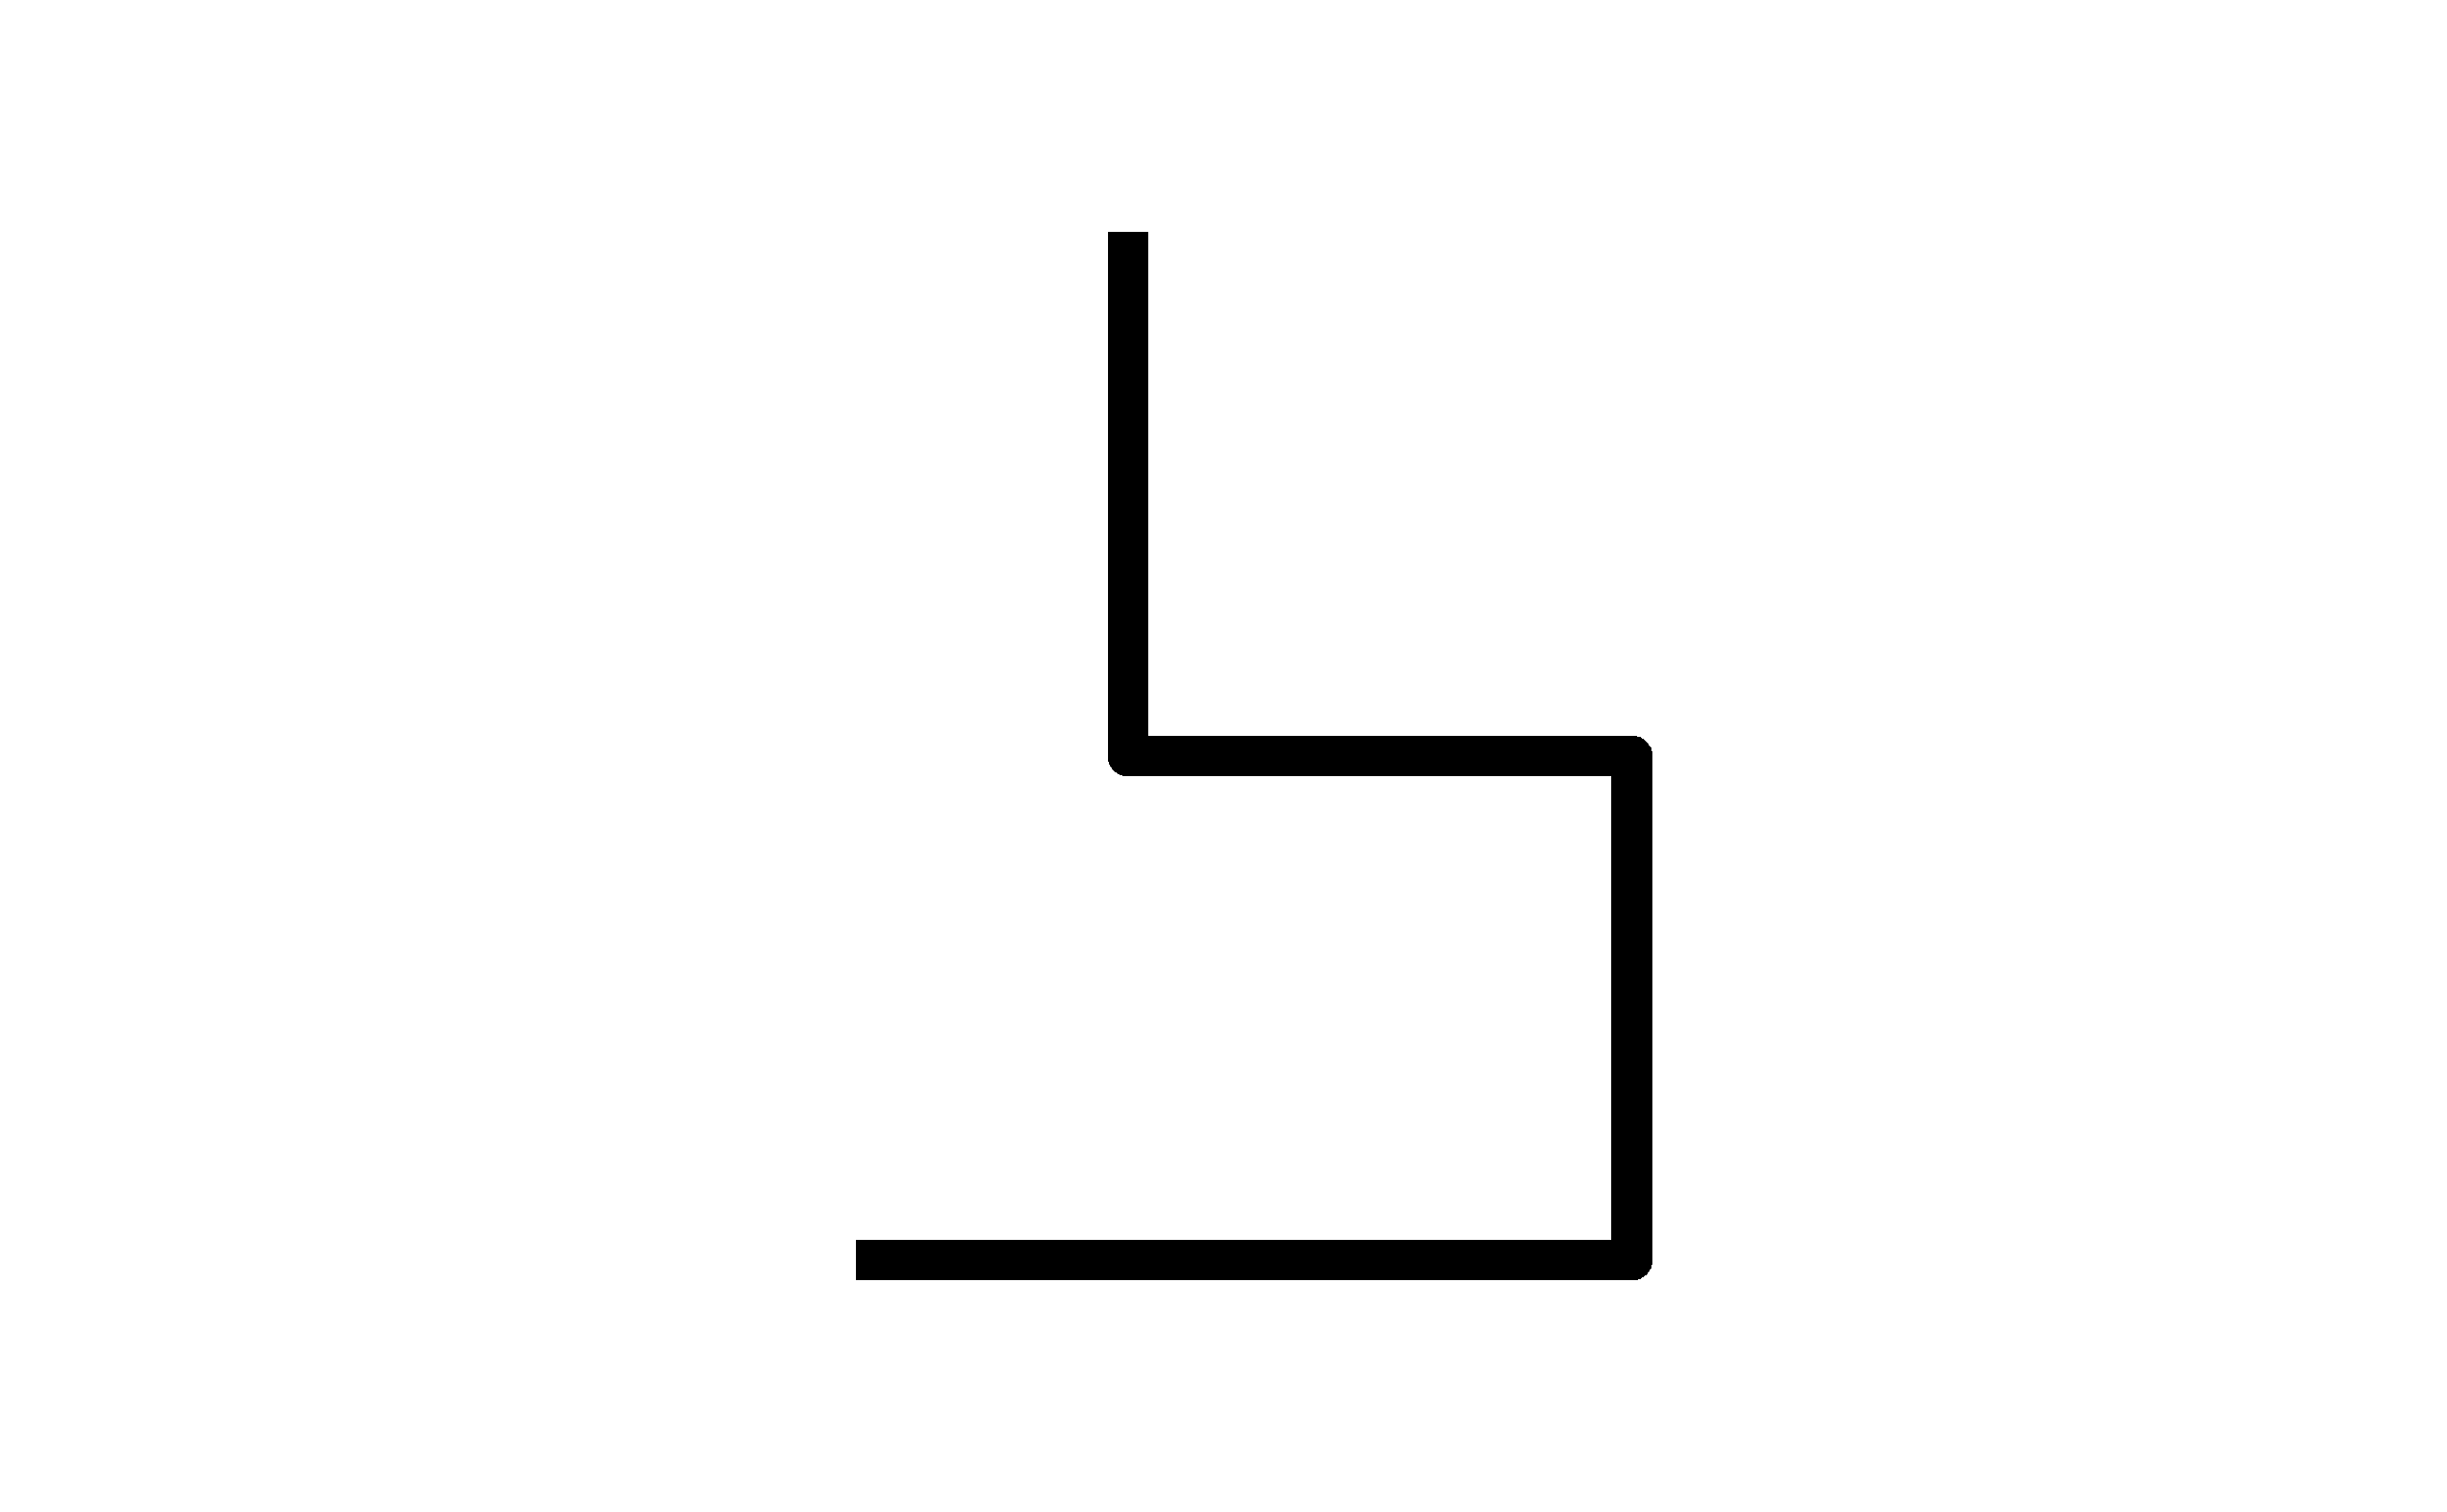
\includegraphics[width=.252\linewidth]{supplement/beta_cluster_example_2/pictures/18/state_cluster_shapes_0.pdf} &
    \includegraphics[width=.252\linewidth]{supplement/beta_cluster_example_2/pictures/18/state_cluster_shapes_1.pdf} & 
    \includegraphics[width=.252\linewidth]{supplement/beta_cluster_example_2/pictures/18/state_cluster_shapes_2.pdf} \\
    \includegraphics[width=.252\linewidth]{supplement/beta_cluster_example_2/pictures/18/state_cluster_shapes_3.pdf} &
    \includegraphics[width=.252\linewidth]{supplement/beta_cluster_example_2/pictures/18/state_cluster_shapes_4.pdf} &
    \includegraphics[width=.252\linewidth]{supplement/beta_cluster_example_2/pictures/18/state_cluster_shapes_5.pdf} 
  \end{tabular}
}
%
Clearly the folding pathway is dominated by the formation of the turn. This implies that the formation of the turn in the $\beta$-hairpin is a nucleation event, a necessary first step for the folding process. 

The folding kinetics can be computed using the quasi-steady-steady approximation. Grouping the intermediate states as $c_\chem{I} = \braces{c_{17}, c_{18}}$, the final state $c_\chem{F} = \braces{c_{11}}$ and all other clusters as random coil states $c_\chem{R}$ we have
%
\inlinembox{Macrostate model for $\beta$-hairpin}{\TIKZbetahairpinMacrostates}
%
The forward and backwards transitions were calculated to be
\begin{equation}
  \B{S} =
  \begin{bmatrix}
    0.54042 & 0.39912 & 0.06046 \\
    0.00713 & 0.99266 & 0.00021 \\
    0.00005 & 0.00001 & 0.99995 \\
  \end{bmatrix}
\end{equation}
with the rows ordered as $\brackets{ c_\chem{R}, c_\chem{I}, c_\chem{F} }$.

We stress that these predicted transitions are a coarse-graining of the real kinetics since we have assumed the states equilibrate before transitioning into a different macrostate. Nevertheless, the approximation is validated by the observation that at the observed temperature, the slowest eigenmodes dominate the kinetics. 

\section {Remarks}

When the number of microstates is large, the eigendecomposition could take an inordinate amount of computation. Thankfully, once $\phi$ is chosen, only the largest eigenpairs need to be found. In general, the full eigendecomposition is unnecessary. There exist techniques like the Lanczos routine that extract only the larger eigenpairs.\cite{komzsik_lanczos_1987} These techniques work well with the matrices used in the MSC algorithm; the Lanczos algorithm works with non-Hermitian matrices and excels when the matrices are sparse and the eigenvalues are not degenerate.

It is worth noting that the macrostates obtained did not use the equations of motion, only the time-series data. This gives the technique  wide applicability, extending beyond the domain of biophysical simulations. While the systems studied here were small, the MSC method should scale well to larger more complicated sets of conformational microstates. The limit of the application appears to be the ability of the researcher to extract meaningful data out of the clusters once they have been found. For example, in a larger off-lattice model of protein folding, the full state space of each of the $3N$ residues' coordinates may be unnecessary. In this case, a relative set of microstates may be more useful, say the $2N-2$ dihedral angles.

It would be interesting to pair the results obtained with studies such as Max Caliber, a variational principle for the dynamics of nonequilibrium statistical mechanics.\cite{stock_maximum_2008,jaynes_minimum_1980} Along similar lines, insight might be gained by comparing the clusters against the so-called `thermodynamic length', a  measure of the distance between equilibrium thermodynamics states. This is a Riemannian metric that defines the distance between two states as the number of natural fluctuations along that path.\cite{crooks_measuring_2007} Here the fluctuations are defined through the metric $\B{g}_{ij}$
\begin{equation}
\B{g}_{ij}  = \pfrac{\avg{X_i}}{\lambda^j} = \avg{(X_i-\avg{X_i})(X_j-\avg{X_j})}
\end{equation}
where the $\lambda$'s are the time dependent and configuration independent conjugate variables and the $X$'s are the time independent functions of the configurations (\eg in an isothermal-isobaric ensemble $X$ would contain the internal energy and volume and $\lambda$ would contain the temperature and pressure). The length of a curve parametrized by $t$, from $0$ to $\tau$ is
\begin{equation}
\mathcal{L} = \int_0^\tau \sqrt{\frac{d \lambda^i}{dt} \B{g}_{ij} \frac{d \lambda^j}{dt} } dt
\end{equation}
Since the integration is path-dependent, minimized paths provide a variational approach to important relaxation properties of the system. It is possible that the clusters defined here have a natural connection to this length, perhaps as a first order approximation.


  %CHAPTER: Conclusion
  \chapter{Final Remarks}
%
In this thesis, we have developed several new methods and models, each an attempt to provide insight into the role of entropy in the protein folding process. These studies and others like it, are paramount to a full understanding of protein models. The breadth of the research chapters, depletion forces, crowding, aggregation, and macrostate clustering, emphasizes the fact that protein folding process is still very much an open problem. 

Each of the four research chapters highlight particular suggestions for model improvements, but there are a few overarching directions that seem to be common to all of them. First and foremost, we can't underestimate the need for more comparisons with experimental data. While Chapters \ref{chap:entropic_force} and \ref{chap:WL_crowding} were designed around previously measured data, the model theories have only been extrapolated to different systems, but never tested. The models in Chapters \ref{chap:potts_aggregation} and \ref{chap:clustering_kinetics} have yet to be applied and tested by experimental data outside of a few small systems. This presents an opportunity for both new experimental measurements and extensions of the models to existing data.

In addition to the experimental connection, many of the models present a simplified treatment of the enthalpic terms. This was motivated by the idea to study the effects of entropy exclusively. Many of the calculations however, would have been much more difficult if a more realistic potential had been used. While we feel that a simplified Hamiltonian can capture the essence of the entropic forces, it does present an incomplete picture of physical reality. While the conclusions may remain the same, the supporting evidence could only be strengthened by a more realistic potential. The smaller more focused studies presented here serve an important role as building blocks for a more complete description of the biophysical process. 

It is quite possible to combine molecular dynamics simulations with some of the  ideas presented here. A first step would be the replacement of the $\Go$-like or \chem{H P C} model with the empirically based residue to residue contact matrix defined by Miyazawa and Jernigan.\cite{miyazawa_rl:empirical_1999} In addition the lattice restriction could be removed, or at very least, extended to more complicated geometries. Independently, the macrostate clustering algorithm can serve as a starting point for molecular dynamic simulations, guiding the research to the salient points in conformational space. The time-series method in Chapter \ref{chap:clustering_kinetics} can be applied to the multitude of molecular dynamics trajectories from other numerical experiments.

Each day, new observations are being made that seem to highlight the importance of an \textit{in vivo} model; crowding and aggregation processes are often incomplete without them. Our study here was an attempt to simplify the process at various levels of complexity, so as to give a deeper understanding of the protein folding problem.

\end{thesis}

\suppressfooter

\bibliography{WL_crowding_paper/WL_lattice_protein,entropic_flow_paper/REF_depletion_force_corrected,bibliographies/bulkref,bibliographies/clustering_kinetics_boston_poster_part.bib,bibliographies/extra.bib,bibliographies/graph_iso.bib}

\appendix % appendix needs to be in its own environment
\restorefooter
\chapter{Macro state approximation to the specific heat}
\label{chap:macrostate_approx}

Often times algorithms such as Wang-Landau (see Section \ref{sec:wang_landau}) have convergence properties proportional to the cardinality of the density of states. For many systems characterized by a low degeneracy in the lowest energy levels, the particular form of the density of states at high energies is not important when calculating derivatives of the partition function. Therefore, we find it useful to approximate these higher energy states as a single macrostate. We derive a result for the error introduced by approximating a portion of the density of states $g(x)$ as a single macro state. While the results presented here are for a continuous one-dimensional density of states, the generalization to higher dimensions or discretized states is straightforward. 

\begin{comment}
It will be quite useful to define a few shorthand functions
\begin{align}
  K_A^B(f(x)) &\equiv \int_A^B f(x) e ^ {-x \beta} dx \\
  J_A^B       &\equiv \int_A^B g(x) dx
\end{align}
For brevity we drop the functional dependence on $x$ if it is clear from the description, $g(x)=g$. The normal partition function is
\begin{equation}
  \Z = K_A^B(g)
\end{equation}
%
\end{comment}

We start with the expression of the partition function, assuming the energy range is continuous and spans the interval $A$ to $B$
\begin{equation}
\Z = \int_A^B g(x) e^{-x\beta} dx
\end{equation}
%
We approximate a small portion of the larger energies as a single macrostate in the interval $B(1-\epsilon)$ to $B$. Over this interval we assume the energy is the constant value $x_E$. The most straightforward choice for $x_E$ is a weighted average over the approximated states
\begin{equation}
x_E = \frac
{ \int_{B(1-\epsilon)}^B x g(x) e^{-x\beta} dx }
{\int_{B(1-\epsilon)}^B g(x) e^{-x\beta} dx }
\end{equation}
The approximated form of the partition function becomes
\begin{align}
\Z_\epsilon &= 
\int_A^{B(1-\epsilon)} g(x) e^{-x\beta} dx + 
\int_{B(1-\epsilon)}^B g(x) e^{-x_E\beta} dx \\
&=
\label{eq:macrostate_Zepsilon}
\int_A^{B(1-\epsilon)} g(x) e^{-x\beta} dx + 
e^{-x_E\beta} \int_{B(1-\epsilon)}^B g(x) dx
\end{align}
%
From here, we can ask how accurate this approximation is. By considering small $\epsilon$ from the term $B(1-\epsilon)$, we take a Taylor expansion around $\epsilon=0$,
\begin{equation}
  \Z_\epsilon = \sum \frac{\epsilon^n}{n!}
  \brackets{ \pfrac{\Z_\epsilon}{\epsilon^n}  }
  _ {\epsilon=0}
\end{equation}
When evaluated, this has the surprising result that the first two non-constant terms are zero
\begin{equation}
  \Z_\epsilon = \Z \epsilon^0 + 0 \epsilon^1 + 0 \epsilon^2 + \Delta \epsilon^3 + O(\epsilon^4)
\end{equation}
implying that our approximation is very good indeed.\footnote{In order to take the derivatives we recall that taking the derivative over the limits of integration can be done by
\begin{align}
\pfrac{}{a} \int_{g(a)}^b f(x) dx
=&
\pfrac{}{a} \brackets{F(b) - F(g(a))} \\
=&
- \paren{ \evalat{\frac{d F(t)}{dt}}_{t=g(a)}  } \paren{\frac{d g(a)}{d a} } \\
=&
- f(g(a)) \paren{\frac{d g(a)}{d a} }
\end{align}
where $F$ is the antiderivative of $f$.}
%
The third order term is
\begin{align}
  \Delta = 
  -\frac{B^3 g(B) e^{-B \beta}\beta^2}{24}
\end{align}
%
At very high temperatures we can approximate $\Delta$ by expanding around $\beta=0$
\begin{equation}
  \lim_{\beta\rightarrow 0} \Delta =   -\frac{B^3 g(B) \beta^2}{24} + O(\beta^3)
\end{equation}
%
If we have the explicit form for the density of states such as $g(x) = e^{\gamma x}$ (typically for Ising like systems) we can compute the expansion around $\epsilon$ to many more terms
\begin{align}
\Z_\epsilon( g(x) = e^{\gamma x} ) &= \Z \\ \notag
&-
(1/24) B^3 e^{B(\gamma-\beta)}\beta^2 \epsilon^3 \\ \notag
&+
(1/48)B^4\beta^2e^{B(\gamma-\beta)}(\gamma-\beta)\epsilon^4 \\ \notag
&- 
(1/5760)B^5\beta^2e^{B(\gamma-\beta)}(-72\beta\gamma+33\beta^2+28\gamma^2)\epsilon^5+ \\ \notag
&+ 
(1/11520)B^6\beta^2e^{B(\gamma-\beta)}(45\beta^2\gamma-40\beta\gamma^2+8\gamma^3-13\beta^3)\epsilon^6
+ O(\epsilon^7)
\end{align}
%

\subsubsection{Worked Example : Gaussian DOS}

To illustrate the power of the method we show an example at various levels of approximation. We choose a density of states that is shaped like a Gaussian, \ie a high degeneracy of intermediate states and a low probability of the extreme energies. This is characteristic of the standard Ising model; roughly, an inverted parabolic shape is found when the log of the density of states is plotted against the energies of the system. The chosen Hamiltonian is linear, again in connection with the Ising model. For convenience and clarity in plotting, we shift all energies by a constant factor $\mu=6$, so that the largest accessible state has zero energy
%
\begin{align}
  \HAM(x) &= 
  \begin{cases}
    x-\mu & 0 \le x \le \mu \\
    \infty & \text{otherwise}
  \end{cases} \\
  g(x) &= \exp  \paren{ \frac{-(x-\mu)^2}{2} }
\end{align}
In Figures \ref{fig:macrostate_ex_cut_5}, \ref{fig:macrostate_ex_cut_4}, 
\ref{fig:macrostate_ex_cut_3}, \ref{fig:macrostate_ex_cut_2}, we have plotted the approximate specific heat $CV_\epsilon$ against the exact value as a function of $\beta$. The leftmost graph shows the area of the density states that was considered a single macrostate. At low values of $\epsilon$ the approximation is nearly indistinguishable from the exact curve. In Figure \ref{fig:macrostate_ex_cut_3}, $\epsilon=\frac{1}{2}$, that we have approximated half of the state space \emph{as a single macrostate} and still achieved a reasonable approximation to the specific heat. However, if $\epsilon$ is pushed to high the resulting approximations eventually break down, ultimately creating new spurious phase changes (Figure \ref{fig:macrostate_ex_cut_2}).
%
\begin{figure}[ht]
  \includegraphics[width=\textwidth]{supplement/macrostate_approx_example/pictures/macrostate_epsilon_0211664312906_5.pdf}
  \caption{$CV_{\epsilon}$ with $\epsilon = 1/6$. Approximately $2.1\%$ of $g(x)$ is considered as a single macrostate (see text for details). }
  \label{fig:macrostate_ex_cut_5}
\end{figure}
%
\begin{figure}[ht]
  \includegraphics[width=\textwidth]{supplement/macrostate_approx_example/pictures/macrostate_epsilon_153664915749_4.pdf}
  \caption{$CV_{\epsilon}$ with $\epsilon = 1/3$. Approximately $15.7\%$ of $g(x)$ is considered as a single macrostate (see text for details). }
  \label{fig:macrostate_ex_cut_4}
\end{figure}
%
\begin{figure}[ht]
  \includegraphics[width=\textwidth]{supplement/macrostate_approx_example/pictures/macrostate_epsilon_488131536823_3.pdf}
  \caption{$CV_{\epsilon}$ with $\epsilon = 1/2$. $50.0\%$ of $g(x)$ is considered as a single macrostate (see text for details). }
  \label{fig:macrostate_ex_cut_3}
\end{figure}
%
\begin{figure}[ht]
  \includegraphics[width=\textwidth]{supplement/macrostate_approx_example/pictures/macrostate_epsilon_829972199084_2.pdf}
  \caption{$CV_{\epsilon}$ with $\epsilon = 2/3$. Approximately $84.2\%$ of $g(x)$ is considered as a single macrostate (see text for details). }
  \label{fig:macrostate_ex_cut_2}
\end{figure}


\end{document}
